\documentclass[lang=cn,10pt,chinese]{elegantbook}

\title{AdS/CFT 对偶}

\author{真田信繁}
\institute{Your Institute}
\date{\today}
\bioinfo{主题}{AdS/CFT 对偶}

\extrainfo{量子引力与量子场论的统一框架}

\setcounter{tocdepth}{3}

% 额外的宏包
\usepackage{tikz}
\usetikzlibrary{arrows.meta,decorations.pathmorphing,backgrounds,positioning,calc}
\usepackage[compat=1.1.0]{tikz-feynman}
\usepackage{subcaption}
\usepackage{physics}
\usepackage{braket}
\tikzset{every picture/.style={line width=0.75pt}}

% 参考文献资源
\addbibresource{reference.bib}
\ExecuteBibliographyOptions{sorting=none}

\begin{document}

\maketitle
\frontmatter

\tableofcontents

\mainmatter
%=============================================================================
% 第一部分：基础理论
%=============================================================================

\chapter{引言 (Introduction)}

\section{历史背景与动机}

AdS/CFT 对偶是现代理论物理中最深刻的发现之一，它揭示了引力理论与量子场论之间看似不可能的等价关系。这个对偶最初由 Maldacena 于 1997 年在研究 D3-膜的低能有效理论时发现 \cite{Maldacena1997}，随后由 Gubser、Klebanov、Polyakov \cite{Gubser1998} 和 Witten \cite{Witten1998} 独立给出了具体的计算规则（即 GKPW 关系），建立了 $(d+1)$ 维反德西特时空中的引力理论与其边界上的 $d$ 维共形场论之间的深刻对偶关系。

这个对偶的核心可以用配分函数的等价性来刻画：
\begin{equation}
    Z_{\text{CFT}}[\phi_0] = Z_{\text{gravity}}[\phi \to \phi_0 \text{ at boundary}],
\end{equation}
其中 $\phi_0$ 是边界上的源函数，$\phi$ 是体空间中的场。这个等式意味着：一个引力理论可以等价地用一个没有引力的量子场论来描述。

\section{全息原理的起源}

AdS/CFT 对偶的思想源于全息原理（holographic principle），后者最早由 't Hooft 和 Susskind 提出。全息原理的动机来自黑洞热力学：1970 年代，Bekenstein 和 Hawking 发现黑洞的熵与其视界面积成正比，$S_{\rm BH} = A/(4G_N)$ \cite{Bekenstein1973, Hawking1975}，而非通常的体积。这一面积律暗示引力系统的全部信息可以被编码在其边界上，正如全息图将三维信息编码在二维表面上。

\section{AdS/CFT 的意义}

AdS/CFT 对偶在多个领域具有深远影响：
\begin{itemize}
    \item \textbf{量子引力}：为量子引力提供了一个非微扰的定义——通过边界 CFT 来定义体空间中的量子引力理论
    \item \textbf{强耦合量子场论}：通过强弱对偶，将强耦合问题转化为弱耦合的经典引力计算
    \item \textbf{黑洞物理}：为黑洞信息悖论提供了新的视角，并导致了量子极小曲面和量子纠错等新概念的发现
    \item \textbf{凝聚态物理}：全息超导体 \cite{Hartnoll2008} 和全息非费米液体等模型为强耦合凝聚态系统提供了新的理论工具
    \item \textbf{夸克-胶子等离子体}：$\eta/s = 1/(4\pi)$ 的预言 \cite{Kovtun2005} 与 RHIC 和 LHC 的实验观测惊人一致
\end{itemize}

\section{本文结构}
本文旨在从统计物理的基本概念出发，逐步引导读者理解 AdS/CFT 对偶的核心思想和主要应用。全文组织如下：
\begin{itemize}
    \item \textbf{第一部分（第 2-4 章）：基础理论}——统计物理中的配分函数揭示了微观与宏观之间的桥梁；量子场论中的配分函数作为生成泛函包含了所有关联函数的信息；应力张量作为能量-动量的流密度，在共形场论和 AdS/CFT 中都扮演着核心角色
    \item \textbf{第二部分（第 5-6 章）：AdS 空间与 CFT}——反德西特空间的几何性质（等距群 $SO(2,d)$）与共形场论的对称性（共形群 $SO(2,d)$）精确匹配，这是 AdS/CFT 对偶的对称性基础
    \item \textbf{第三部分（第 7-8 章）：AdS/CFT 对偶与引力配分函数}——GKPW 关系 \cite{Gubser1998, Witten1998} 将 CFT 的生成泛函与引力配分函数联系起来；全息重整化程序 \cite{Henningson1998, Balasubramanian1999} 给出了有限的物理量
    \item \textbf{第四部分（第 9-13 章）：应用}——纠缠熵的全息公式 \cite{Ryu2006} 揭示了量子信息与引力几何的深刻联系；重整化群流的不可逆性由 $c$-定理 \cite{Zamolodchikov1986} 和 $a$-定理 \cite{Komargodski2011} 刻画；强耦合 QCD、相变理论和流体动力学是 AdS/CFT 的重要应用领域
    \item \textbf{第五部分（第 14 章）：总结与展望}——回顾主要结果并讨论未来研究方向
\end{itemize}

%=============================================================================
% 第一部分：基础理论
%=============================================================================

\chapter{统计物理中的配分函数 (Partition Functions in Statistical Physics)}

%=============================================================================

配分函数（partition function）是统计物理中最核心的概念之一。它是一个数学对象，包含了系统的所有热力学信息。一旦我们知道了配分函数，就可以通过微分运算得到所有热力学量，如内能、熵、自由能等。在本节中，我们将从经典统计力学出发，逐步介绍配分函数的概念，然后推广到量子统计力学，最后介绍路径积分（path integral）表述，这是连接统计物理与量子场论（quantum field theory）的桥梁。

\section{统计力学的基本概念}

统计力学是连接微观物理学和宏观热力学的桥梁。它的基本思想是：宏观系统的热力学性质是大量微观粒子集体行为的统计平均结果。

\begin{definition}[微观状态与宏观状态]
\textbf{微观状态}（microstate）描述系统中每个粒子的详细状态。对于经典系统，微观状态由所有粒子的位置坐标 $q_i$ 和动量 $p_i$ 给出；对于量子系统，微观状态由系统的量子态 $|\psi\rangle$ 描述。

\textbf{宏观状态}（macrostate）描述系统的宏观可观测量，如温度 $T$、压强 $P$、体积 $V$、内能 $E$ 等。一个宏观状态通常对应大量微观状态。
\end{definition}

\begin{definition}[热力学极限]
当粒子数 $N \to \infty$ 和体积 $V \to \infty$，但粒子数密度 $N/V$ 保持有限时的极限称为\textbf{热力学极限}（thermodynamic limit）。在热力学极限下，涨落可以忽略不计，热力学描述变得精确。
\end{definition}

\begin{note}
统计力学的基本假设是\textbf{等概率原理}（equal a priori probability principle）：对于一个孤立系统，所有满足宏观约束的微观状态出现的概率相等。这个假设是统计力学的基石，虽然它不能从更基本的原理推导出来，但它的推论与实验高度一致。
\end{note}

\section{统计系综}

统计系综（statistical ensemble）是描述系统概率分布的数学框架。它是大量相同系统的集合，每个系统都处于相同的宏观条件下，但可能处于不同的微观状态。图 \ref{fig:ensembles} 展示了三种主要统计系综的示意图。

\begin{figure}[htbp]
\centering
\begin{subfigure}[b]{0.3\textwidth}
\centering
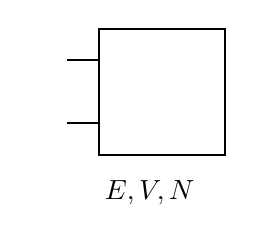
\begin{tikzpicture}[scale=0.8]
    \draw[thick] (0,0) rectangle (2,2);
    \node at (1,1) {系统};
    \draw[thick] (0,0.5) -- (-0.5,0.5);
    \draw[thick] (0,1.5) -- (-0.5,1.5);
    \node at (-0.8,1) {绝热壁};
    \node at (1,-0.3) {微正则系综};
    \node at (1,-0.6) {$E, V, N$ 固定};
\end{tikzpicture}
\end{subfigure}
\hfill
\begin{subfigure}[b]{0.3\textwidth}
\centering
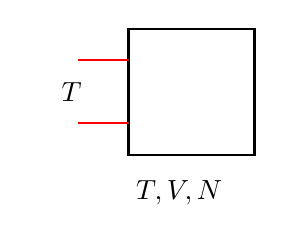
\begin{tikzpicture}[scale=0.8]
    \draw[thick] (0,0) rectangle (2,2);
    \node at (1,1) {系统};
    \draw[thick, red] (0,0.5) -- (-0.8,0.5);
    \draw[thick, red] (0,1.5) -- (-0.8,1.5);
    \node at (-1.1,1) {热库 $T$};
    \node at (1,-0.3) {正则系综};
    \node at (1,-0.6) {$T, V, N$ 固定};
\end{tikzpicture}
\end{subfigure}
\hfill
\begin{subfigure}[b]{0.3\textwidth}
\centering
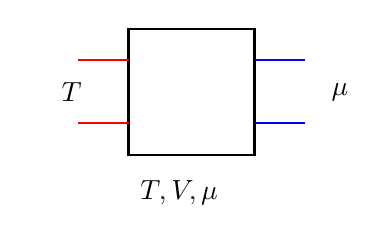
\begin{tikzpicture}[scale=0.8]
    \draw[thick] (0,0) rectangle (2,2);
    \node at (1,1) {系统};
    \draw[thick, red] (0,0.5) -- (-0.8,0.5);
    \draw[thick, red] (0,1.5) -- (-0.8,1.5);
    \node at (-1.1,1) {热库 $T$};
    \draw[thick, blue] (2,0.5) -- (2.8,0.5);
    \draw[thick, blue] (2,1.5) -- (2.8,1.5);
    \node at (3.1,1) {粒子库 $\mu$};
    \node at (1,-0.3) {巨正则系综};
    \node at (1,-0.6) {$T, V, \mu$ 固定};
\end{tikzpicture}
\end{subfigure}
\caption{三种主要统计系综的示意图。从左到右：微正则系综（孤立系统）、正则系综（与热库接触）、巨正则系综（与热库和粒子库接触）。}
\label{fig:ensembles}
\end{figure}

\begin{definition}[微正则系综]
\textbf{微正则系综}（microcanonical ensemble）描述孤立系统，能量 $E$ 固定。系统处于每个微观状态的概率相等（等概率原理）：
\begin{equation}
    \rho = \frac{1}{\Omega(E)} \delta(H - E),
\end{equation}
其中 $\Omega(E)$ 是能量为 $E$ 的微观状态数，$\rho$ 是概率密度函数。熵定义为：
\begin{equation}
    S = k_B \ln \Omega(E),
\end{equation}
这就是著名的玻尔兹曼熵公式。$k_B$ 是玻尔兹曼常数（Boltzmann constant），$k_B \approx 1.381 \times 10^{-23}$ J/K。
\end{definition}

\begin{definition}[正则系综]
\textbf{正则系综}（canonical ensemble）描述与热库接触的系统，温度 $T$ 固定。系统处于能量为 $E_i$ 的微观状态的概率为：
\begin{equation}
    p_i = \frac{e^{-\beta E_i}}{Z},
\end{equation}
其中 $\beta = 1/(k_B T)$ 是逆温度（inverse temperature），$Z$ 是配分函数（partition function）：
\begin{equation}
    Z = \sum_i e^{-\beta E_i}.
\end{equation}
这个概率分布称为玻尔兹曼分布（Boltzmann distribution）。
\end{definition}

\begin{definition}[巨正则系综]
\textbf{巨正则系综}（grand canonical ensemble）描述与粒子库和热库接触的系统，温度 $T$ 和化学势 $\mu$ 固定。系统处于粒子数为 $N$、能量为 $E_i$ 的微观状态的概率为：
\begin{equation}
    p_i = \frac{e^{-\beta (E_i - \mu N)}}{\mathcal{Z}},
\end{equation}
其中 $\mathcal{Z}$ 是巨配分函数（grand partition function）：
\begin{equation}
    \mathcal{Z} = \sum_{N=0}^{\infty} \sum_i e^{-\beta (E_i - \mu N)} = \sum_{N=0}^{\infty} z^N Z_N,
\end{equation}
其中 $z = e^{\beta \mu}$ 是逸度（fugacity），$Z_N$ 是粒子数为 $N$ 时的正则配分函数。
\end{definition}

\begin{property}[系综等价性]
\textbf{系综等价性}（ensemble equivalence）：在热力学极限下，不同系综给出相同的热力学性质。这意味着我们可以根据方便选择任何一个系综来计算。
\end{property}

\begin{remark}
系综等价性的物理原因在于：在热力学极限下，相对涨落按 $1/\sqrt{N}$ 趋于零。因此，固定粒子数 $N$（正则系综）与允许粒子数涨落（巨正则系综）的差别可以忽略。但在有限系统或临界点附近，系综等价性可能失效，此时必须谨慎选择系综。
\end{remark}

\section{经典统计力学}

考虑一个由 $N$ 个粒子组成的经典系统。每个粒子的位置坐标为 $q_i$，动量为 $p_i$（其中 $i = 1, 2, \ldots, N$）。系统的总能量由哈密顿量（Hamiltonian）$H(q, p)$ 给出，它是所有粒子的坐标和动量的函数。

\begin{definition}[相空间]
\textbf{相空间}（phase space）：由所有粒子的位置和动量张成的 $6N$ 维空间。相空间中的一个点代表系统的一个微观状态。
\end{definition}

\begin{definition}[哈密顿量]
\textbf{哈密顿量}（Hamiltonian）：系统的总能量，通常是动能和势能之和：
\begin{equation}
    H(q, p) = \sum_{i=1}^{N} \frac{p_i^2}{2m} + V(q_1, \ldots, q_N),
\end{equation}
其中第一项是动能，$V$ 是势能。
\end{definition}

在正则系综中，系统与一个温度为 $T$ 的热库（heat bath）接触。根据玻尔兹曼分布（Boltzmann distribution），系统处于某个微观状态 $(q, p)$ 的概率与 $e^{-\beta H(q, p)}$ 成正比。

\begin{theorem}[经典正则配分函数]
\textbf{配分函数}定义为所有可能微观状态的玻尔兹曼因子之和。对于经典系统，这个"求和"实际上是相空间（phase space）上的积分：
\begin{equation}
    Z = \int \frac{d^N q \, d^N p}{h^{3N} N!} e^{-\beta H(q, p)}.
    \label{eq:classical_Z}
\end{equation}
其中：
\begin{itemize}
    \item $d^N q \, d^N p$ 表示对整个相空间积分，$d^N q = dq_1 \cdots dq_N$，$d^N p = dp_1 \cdots dp_N$
    \item $h$ 是普朗克常数（Planck constant），$h \approx 6.626 \times 10^{-34}$ J$\cdot$s。除以 $h^{3N}$ 是为了使配分函数无量纲化，这来自于量子力学中相空间体积元的最小单位
    \item $N!$ 是全同粒子的修正，这是因为交换两个全同粒子不产生新的微观状态。如果不除以 $N!$，会导致熵不是广延量，这就是著名的吉布斯佯谬（Gibbs paradox）
\end{itemize}
\end{theorem}

\begin{note}
配分函数 $Z$ 是所有可能微观状态的"统计权重"的总和。能量越低的状态，其玻尔兹曼因子 $e^{-\beta E}$ 越大，因此对配分函数的贡献越大。温度越低（$\beta$ 越大），低能状态的相对权重越大。
\end{note}

\begin{property}[非相互作用系统的配分函数分解]
如果系统的哈密顿量可以分解为独立部分之和 $H = H_1 + H_2 + \cdots + H_N$（即各部分之间无相互作用），则配分函数分解为各部分配分函数的乘积：
\begin{equation}
    Z = Z_1 \cdot Z_2 \cdots Z_N = \prod_{i=1}^N Z_i,
\end{equation}
其中 $Z_i = \int \frac{dq_i \, dp_i}{h} e^{-\beta H_i}$。相应地，自由能具有可加性：$F = F_1 + F_2 + \cdots + F_N$。这一性质大大简化了无相互作用系统（如理想气体）的计算。
\end{property}

\begin{example}[经典理想气体的配分函数]
对于 $N$ 个无相互作用的经典粒子，哈密顿量仅为动能之和。由于动能与位置无关，配分函数可以分解为动量部分和位置部分：
\begin{equation}
    Z = \frac{1}{N! h^{3N}} \left(\int d^3q \right)^N \left(\int d^3p \, e^{-\beta p^2/(2m)}\right)^N = \frac{V^N}{N!} \left(\frac{2\pi m}{\beta h^2}\right)^{3N/2}.
\end{equation}
这展示了配分函数如何将微观力学（哈密顿量）与宏观热力学（通过 $\beta$）联系起来。
\end{example}

\section{热力学量的推导}

\begin{theorem}[热力学量与配分函数]
一旦知道了配分函数，所有热力学量都可以从它推导出来。配分函数之所以如此重要，是因为它是一个"生成函数"：通过对它进行适当的微分运算，我们可以得到所有感兴趣的物理量。

\textbf{亥姆霍兹自由能}（Helmholtz free energy）$F$：
\begin{equation}
    F = -k_B T \ln Z = -\frac{1}{\beta} \ln Z.
\end{equation}
自由能的物理意义是：在等温等容过程中，系统对外做的最大功等于自由能的减少。自由能是热力学势（thermodynamic potential），它以温度 $T$ 和体积 $V$ 为自然变量。

从自由能出发，我们可以得到其他热力学量：

\textbf{熵}（entropy）$S$：
\begin{equation}
    S = -\left(\frac{\partial F}{\partial T}\right)_V = k_B (\ln Z + \beta E).
\end{equation}
熵是系统无序程度的度量。根据热力学第二定律，孤立系统的熵永不减少。

\textbf{内能}（internal energy）$E$：
\begin{equation}
    E = -\frac{\partial}{\partial \beta} \ln Z = \langle H \rangle = \sum_i p_i E_i.
\end{equation}
内能是系统能量的统计平均值。

\textbf{压强}（pressure）$P$：
\begin{equation}
    P = -\left(\frac{\partial F}{\partial V}\right)_T = \frac{1}{\beta} \frac{\partial \ln Z}{\partial V}.
\end{equation}
压强是系统对体积变化的响应。

\textbf{比热容}（heat capacity）$C_V$：
\begin{equation}
    C_V = \left(\frac{\partial E}{\partial T}\right)_V = k_B \beta^2 \left( \langle H^2 \rangle - \langle H \rangle^2 \right) = k_B \beta^2 \langle (\Delta H)^2 \rangle.
\end{equation}
比热容度量系统吸收热量的能力，它与能量涨落成正比。

\textbf{化学势}（chemical potential）$\mu$：
\begin{equation}
    \mu = -T \left(\frac{\partial S}{\partial N}\right)_{E,V} = \left(\frac{\partial F}{\partial N}\right)_{T,V}.
\end{equation}
化学势度量增加一个粒子时系统自由能的变化。
\end{theorem}

\begin{proof}[热力学量从配分函数推导的证明]
我们证明内能 $E = -\partial \ln Z / \partial \beta$。由配分函数的定义 $Z = \sum_i e^{-\beta E_i}$，对 $\beta$ 求导：
\begin{equation}
    \frac{\partial Z}{\partial \beta} = \sum_i (-E_i) e^{-\beta E_i},
\end{equation}
因此
\begin{equation}
    \frac{\partial \ln Z}{\partial \beta} = \frac{1}{Z} \frac{\partial Z}{\partial \beta} = -\frac{1}{Z} \sum_i E_i e^{-\beta E_i} = -\sum_i E_i p_i = -\langle H \rangle = -E.
\end{equation}
这就证明了 $E = -\partial \ln Z / \partial \beta$。

接下来证明自由能 $F = -k_B T \ln Z$ 与热力学的关系。在正则系综中，概率分布 $p_i = e^{-\beta E_i}/Z$ 最大化了信息熵 $S = -k_B \sum_i p_i \ln p_i$，约束条件为 $\sum_i p_i = 1$ 和 $\sum_i p_i E_i = E$。利用拉格朗日乘子法，可以证明自由能 $F = E - TS$ 满足 $F = -k_B T \ln Z$。具体地，将 $p_i = e^{-\beta E_i}/Z$ 代入熵的表达式：
\begin{equation}
    S = -k_B \sum_i p_i (-\beta E_i - \ln Z) = k_B \beta E + k_B \ln Z = \frac{E - F}{T},
\end{equation}
其中最后一步使用了 $F = -k_B T \ln Z$，从而 $F = E - TS$，这正是亥姆霍兹自由能的标准定义。

比热容的公式可以通过对内能求导得到：
\begin{equation}
    C_V = \frac{\partial E}{\partial T} = \frac{\partial}{\partial T}\left(-\frac{\partial \ln Z}{\partial \beta}\right) = k_B \beta^2 \frac{\partial^2 \ln Z}{\partial \beta^2}.
\end{equation}
利用 $\partial^2 \ln Z / \partial \beta^2 = \langle H^2 \rangle - \langle H \rangle^2$，即得 $C_V = k_B \beta^2 \langle (\Delta H)^2 \rangle$。
\end{proof}

\section{经典例子}

\begin{example}[理想气体]
\textbf{例子 1：理想气体}（ideal gas）。对于 $N$ 个无相互作用的经典粒子，哈密顿量为
\begin{equation}
    H(q, p) = \sum_{i=1}^{N} \frac{p_i^2}{2m}.
\end{equation}
配分函数为：
\begin{equation}
    Z = \frac{1}{N!} \left(\frac{V}{h^3}\right)^N \left(\int d^3 p \, e^{-\beta p^2/(2m)}\right)^N = \frac{1}{N!} \left(\frac{V}{\lambda^3}\right)^N,
\end{equation}
其中 $\lambda = h/\sqrt{2\pi m k_B T}$ 是热德布罗意波长（thermal de Broglie wavelength），它度量量子效应的重要性。

从配分函数可以推导出理想气体的状态方程：
\begin{equation}
    PV = Nk_B T,
\end{equation}
以及内能 $E = \frac{3}{2}Nk_B T$（能量均分定理的结果）和熵（Sackur-Tetrode 公式）：
\begin{equation}
    S = Nk_B \left[ \ln\left(\frac{V}{N\lambda^3}\right) + \frac{5}{2} \right].
\end{equation}
Sackur-Tetrode 公式给出了理想气体的绝对熵，这是经典统计力学的重要成就。
\end{example}

\begin{example}[经典谐振子]
\textbf{例子 2：经典谐振子}（classical harmonic oscillator）。一维经典谐振子的哈密顿量为：
\begin{equation}
    H(q, p) = \frac{p^2}{2m} + \frac{1}{2}m\omega^2 q^2,
\end{equation}
其中 $\omega$ 是角频率。配分函数为：
\begin{equation}
    Z = \frac{1}{h} \int dq \, dp \, e^{-\beta H(q, p)} = \frac{1}{\beta \hbar \omega},
\end{equation}
其中 $\hbar = h/(2\pi)$ 是约化普朗克常数。平均能量为 $E = k_B T$，这就是能量均分定理（equipartition theorem）：每个二次自由度贡献 $k_B T/2$ 的能量。
\end{example}

\begin{example}[二能级系统]
\textbf{例子 3：二能级系统}（two-level system）。考虑一个具有两个能级 $E_0 = 0$ 和 $E_1 = \epsilon$ 的系统。配分函数为：
\begin{equation}
    Z = 1 + e^{-\beta \epsilon}.
\end{equation}
平均能量为：
\begin{equation}
    E = \frac{\epsilon e^{-\beta \epsilon}}{1 + e^{-\beta \epsilon}} = \frac{\epsilon}{e^{\beta \epsilon} + 1}.
\end{equation}
在高温极限（$\beta \epsilon \ll 1$）下，$E \approx \epsilon/2$，两个能级等概率占据；在低温极限（$\beta \epsilon \gg 1$）下，$E \approx \epsilon e^{-\beta \epsilon} \to 0$，系统几乎完全占据基态。
\end{example}

\begin{example}[顺磁性物质]
\textbf{例子 4：顺磁性物质}（paramagnetic substance）。考虑 $N$ 个自旋为 $1/2$ 的粒子置于外磁场 $B$ 中，每个粒子有两个能级 $E_\pm = \mp \mu B$。系统的配分函数为：
\begin{equation}
    Z = \left(2\cosh(\beta\mu B)\right)^N.
\end{equation}
由此可得磁化强度 $M = N\mu\tanh(\beta\mu B)$，在高温下得到居里定律 $M \approx N\mu^2 B/(k_B T)$，即磁化率 $\chi \propto 1/T$。
\end{example}

\section{涨落理论}

在统计力学中，物理量围绕其平均值涨落。涨落的大小可以通过配分函数来计算。

\begin{theorem}[能量涨落与比热容]
\textbf{能量涨落}（energy fluctuation）：
\begin{equation}
    \langle (\Delta E)^2 \rangle = \langle H^2 \rangle - \langle H \rangle^2 = \frac{\partial^2 \ln Z}{\partial \beta^2} = k_B T^2 C_V.
\end{equation}
这个公式表明，能量涨落与比热容成正比。
\end{theorem}

\textbf{相对涨落}（relative fluctuation）：
\begin{equation}
    \frac{\sqrt{\langle (\Delta E)^2 \rangle}}{E} \sim \frac{1}{\sqrt{N}},
\end{equation}
对于宏观系统（$N \sim 10^{23}$），相对涨落可以忽略不计（约为 $10^{-12}$），这就是为什么热力学可以描述宏观系统。

\begin{theorem}[涨落-耗散定理]
\textbf{涨落-耗散定理}（fluctuation-dissipation theorem）：系统对外界扰动的响应（如比热容、磁化率等）与系统内部的涨落成正比。这是统计力学的一个基本定理，它将宏观响应函数与微观涨落联系起来。
\end{theorem}

\textbf{磁化率}（magnetic susceptibility）：对于磁性系统，磁化率 $\chi$ 与磁矩涨落成正比：
\begin{equation}
    \chi = \beta \langle (\Delta M)^2 \rangle = \beta (\langle M^2 \rangle - \langle M \rangle^2).
\end{equation}

\begin{remark}[涨落与相变]
涨落在相变（phase transition）附近起着关键作用\cite{Landau1937}。在临界点附近，关联长度趋于无穷，涨落变得宏观可见，相对涨落不再按 $1/\sqrt{N}$ 趋于零。此时热力学描述失效，必须使用重正化群（renormalization group）方法\cite{Wilson1974}来处理临界现象。
\end{remark}

\section{量子统计力学}

在量子力学中，系统的状态由希尔伯特空间（Hilbert space）中的态矢量 $|\psi\rangle$ 描述，可观测量由厄米算符（Hermitian operator）描述。系统的能量由哈密顿算符（Hamiltonian operator）$\hat{H}$ 的本征值给出：
\begin{equation}
    \hat{H} |n\rangle = E_n |n\rangle,
\end{equation}
其中 $|n\rangle$ 是能量本征态（energy eigenstate），$E_n$ 是对应的能量本征值（energy eigenvalue）。

\begin{definition}[密度矩阵]
\textbf{密度矩阵}（density matrix）：在量子统计力学中，系统的状态由密度矩阵 $\hat{\rho}$ 描述。对于正则系综：
\begin{equation}
    \hat{\rho} = \frac{e^{-\beta \hat{H}}}{Z},
\end{equation}
其中 $Z = \Tr e^{-\beta \hat{H}}$ 是配分函数。
\end{definition}

\begin{theorem}[量子正则配分函数]
\textbf{量子配分函数}定义为玻尔兹曼算符（Boltzmann operator）$e^{-\beta \hat{H}}$ 的迹（trace）：
\begin{equation}
    Z = \Tr e^{-\beta \hat{H}} = \sum_n \langle n | e^{-\beta \hat{H}} | n \rangle = \sum_n e^{-\beta E_n}.
\end{equation}
这里我们使用了能量本征态的完备性关系（completeness relation）$\sum_n |n\rangle \langle n| = \hat{1}$。

\textbf{迹}（trace）的定义：对于任意算符 $\hat{A}$，其迹定义为 $\Tr \hat{A} = \sum_n \langle n | \hat{A} | n \rangle$，其中求和遍及完备基。迹的值不依赖于基的选择。
\end{theorem}

量子配分函数是所有能量本征态的玻尔兹曼因子之和。与经典情况类似，低能态对配分函数的贡献更大。

量子配分函数同样包含了系统的所有热力学信息。自由能、熵、内能等热力学量的表达式与经典情况完全相同：
\begin{align}
    F &= -k_B T \ln Z, \\
    S &= -\left(\frac{\partial F}{\partial T}\right)_V, \\
    E &= -\frac{\partial}{\partial \beta} \ln Z = \frac{\Tr(\hat{H} e^{-\beta \hat{H}})}{\Tr e^{-\beta \hat{H}}} = \sum_n p_n E_n,
\end{align}
其中 $p_n = e^{-\beta E_n}/Z$ 是系统处于能量本征态 $|n\rangle$ 的概率。

\begin{property}[量子配分函数的经典极限]
当温度足够高（$\beta \to 0$）时，量子配分函数趋于经典配分函数。具体地，对于由 $N$ 个粒子组成的系统，量子配分函数在高温极限下满足：
\begin{equation}
    Z_{\text{quantum}} \xrightarrow{\beta \to 0} Z_{\text{classical}} = \frac{1}{N! h^{3N}} \int d^Nq \, d^Np \, e^{-\beta H(q,p)}.
\end{equation}
物理上，这是因为高温下热德布罗意波长 $\lambda = h/\sqrt{2\pi m k_B T}$ 远小于粒子间距，量子统计效应（全同粒子的对称化或反对称化要求）可以忽略，系统行为趋于经典\cite{Landau1937}。
\end{property}

\begin{remark}[量子统计与经典统计的区别]
量子统计力学与经典统计力学的根本区别在于：量子力学中，全同粒子不可区分，且态空间是离散的。对于玻色子，波函数在粒子交换下对称；对于费米子，波函数反对称。这些量子统计效应在低温下变得重要，导致玻色-爱因斯坦凝聚和费米简并等现象。
\end{remark}

\section{量子例子}

\begin{example}[量子谐振子]
\textbf{例子 1：量子谐振子}（quantum harmonic oscillator）。一维量子谐振子的能级为：
\begin{equation}
    E_n = \hbar \omega \left(n + \frac{1}{2}\right), \quad n = 0, 1, 2, \ldots
\end{equation}
其中 $\hbar$ 是约化普朗克常数，$\omega$ 是角频率。注意，最低能级 $E_0 = \hbar\omega/2$ 不为零，这称为零点能（zero-point energy），是量子力学的特征。

配分函数为：
\begin{equation}
    Z = \sum_{n=0}^{\infty} e^{-\beta \hbar \omega (n + 1/2)} = \frac{e^{-\beta \hbar \omega/2}}{1 - e^{-\beta \hbar \omega}} = \frac{1}{2 \sinh(\beta \hbar \omega/2)}.
\end{equation}
平均能量为：
\begin{equation}
    E = \frac{\hbar \omega}{2} + \frac{\hbar \omega}{e^{\beta \hbar \omega} - 1}.
\end{equation}
第一项是零点能，第二项是热激发的贡献。在高温极限（$\beta \hbar \omega \ll 1$）下，$E \approx k_B T$，与经典结果一致；在低温极限（$\beta \hbar \omega \gg 1$）下，$E \approx \hbar\omega/2$，系统冻结在基态。
\end{example}

\begin{example}[量子二能级系统]
\textbf{例子 2：量子二能级系统}。考虑自旋 1/2 粒子在磁场 $B$ 中，能级为 $E_\pm = \pm \mu B$，其中 $\mu$ 是磁矩。配分函数为：
\begin{equation}
    Z = e^{\beta \mu B} + e^{-\beta \mu B} = 2\cosh(\beta \mu B).
\end{equation}
磁化强度为：
\begin{equation}
    M = \frac{1}{\beta} \frac{\partial \ln Z}{\partial B} = \mu \tanh(\beta \mu B).
\end{equation}
在高温极限（$\beta \mu B \ll 1$）下，$M \approx \beta \mu^2 B$，即居里定律（Curie's law）；在低温极限（$\beta \mu B \gg 1$）下，$M \to \mu$，即磁化饱和。
\end{example}

\begin{example}[玻色子和费米子]
\textbf{例子 3：玻色子和费米子}。对于量子理想气体，配分函数取决于粒子的统计性质。

\textbf{玻色子}（bosons）：服从玻色-爱因斯坦统计（Bose-Einstein statistics），自旋为整数。每个单粒子态可以被任意多个玻色子占据。配分函数为：
\begin{equation}
    \ln Z = -\sum_k \ln(1 - e^{-\beta(\epsilon_k - \mu)}),
\end{equation}
其中 $\epsilon_k$ 是单粒子能级，$\mu$ 是化学势。平均占据数为玻色-爱因斯坦分布：
\begin{equation}
    \langle n_k \rangle = \frac{1}{e^{\beta(\epsilon_k - \mu)} - 1}.
\end{equation}

\textbf{费米子}（fermions）：服从费米-狄拉克统计（Fermi-Dirac statistics），自旋为半整数。每个单粒子态最多被一个费米子占据（泡利不相容原理）。配分函数为：
\begin{equation}
    \ln Z = \sum_k \ln(1 + e^{-\beta(\epsilon_k - \mu)}).
\end{equation}
平均占据数为费米-狄拉克分布：
\begin{equation}
    \langle n_k \rangle = \frac{1}{e^{\beta(\epsilon_k - \mu)} + 1}.
\end{equation}
\end{example}

\begin{example}[玻色-爱因斯坦凝聚]
\textbf{例子 4：玻色-爱因斯坦凝聚}（Bose-Einstein condensation，BEC）。考虑一个由 $N$ 个无相互作用玻色子组成的系统，处于体积为 $V$ 的盒子中。当温度降低到临界温度 $T_c$ 以下时，宏观量的粒子会凝聚到能量最低的单粒子态（基态），这就是玻色-爱因斯坦凝聚。图 \ref{fig:bec} 展示了 BEC 的能级占据示意图。

\begin{figure}[htbp]
\centering
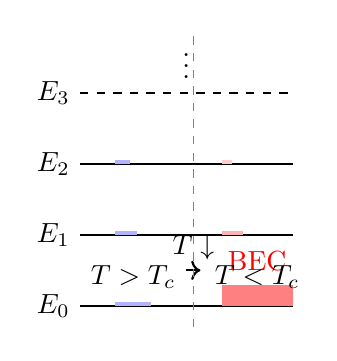
\begin{tikzpicture}[scale=0.9]
    % 能级
    \draw[thick] (0,0) -- (3,0);
    \node[left] at (0,0) {$E_0$};
    \draw[thick] (0,1) -- (3,1);
    \node[left] at (0,1) {$E_1$};
    \draw[thick] (0,2) -- (3,2);
    \node[left] at (0,2) {$E_2$};
    \draw[thick, dashed] (0,3) -- (3,3);
    \node[left] at (0,3) {$E_3$};
    \node at (1.5,3.5) {$\vdots$};
    % 高温占据
    \fill[blue!30] (0.5,0) rectangle (1.0,0.05);
    \fill[blue!30] (0.5,1) rectangle (0.8,1.05);
    \fill[blue!30] (0.5,2) rectangle (0.7,2.05);
    \node[below] at (0.75,-0.1) {\small 各能级均匀占据};
    % 低温占据
    \fill[red!50] (2.0,0) rectangle (3.0,0.3);
    \fill[red!30] (2.0,1) rectangle (2.3,1.05);
    \fill[red!20] (2.0,2) rectangle (2.15,2.05);
    \node[below] at (2.5,-0.1) {\small 宏观占据基态};
    % 箭头
    \draw[->, thick] (1.5,0.5) -- (1.7,0.5);
    \node[above] at (1.6,0.5) {$T \downarrow$};
    % BEC 标注
    \node[above, red] at (2.5,0.35) {BEC};
    \node[above] at (0.75,0.1) {$T > T_c$};
    \node[above] at (2.5,0.1) {$T < T_c$};
    % 分隔线
    \draw[thin, gray, dashed] (1.6,-0.3) -- (1.6,3.8);
\end{tikzpicture}
\caption{玻色-爱因斯坦凝聚的能级占据示意图。左：$T > T_c$ 时，粒子按玻色-爱因斯坦分布在各能级上；右：$T < T_c$ 时，宏观量粒子凝聚到基态 $E_0$。}
\label{fig:bec}
\end{figure}

临界温度为：
\begin{equation}
    T_c = \frac{2\pi \hbar^2}{m k_B}\left(\frac{N}{V \zeta(3/2)}\right)^{2/3},
\end{equation}
其中 $\zeta(3/2) \approx 2.612$ 是黎曼 $\zeta$ 函数的值。在 $T < T_c$ 时，基态粒子数为：
\begin{equation}
    N_0 = N\left[1 - \left(\frac{T}{T_c}\right)^{3/2}\right].
\end{equation}
BEC 是量子统计力学最深刻的预言之一，1995 年在超冷原子气体中首次实验观测到。

\begin{note}[BEC 的物理意义]
玻色-爱因斯坦凝聚的发生可以通过热德布罗意波长来理解。当 $\lambda \sim n^{-1/3}$（即粒子间距与波长可比）时，不同粒子的波函数开始重叠，量子统计效应变得重要。此时粒子"失去个体性"，形成宏观量子态。BEC 在超导（库珀对凝聚）和超流现象中起着核心作用。
\end{note}
\end{example}

\section{路径积分表述}

路径积分（path integral）是量子力学的一种等价表述，由费曼（Feynman）于 1948 年提出。它的核心思想是：一个粒子从初态到末态的跃迁振幅（transition amplitude）等于所有可能路径的贡献之和。

\begin{definition}[传播子]
\textbf{传播子}（propagator）：粒子从位置 $q_i$ 在时间 $t_i$ 传播到位置 $q_f$ 在时间 $t_f$ 的振幅为：
\begin{equation}
    K(q_f, t_f; q_i, t_i) = \langle q_f | e^{-i\hat{H}(t_f - t_i)/\hbar} | q_i \rangle = \int \mathcal{D}q(t) \, e^{iS[q]/\hbar},
\end{equation}
其中 $S[q] = \int_{t_i}^{t_f} dt \, L(q, \dot{q})$ 是经典作用量，$L$ 是拉格朗日量（Lagrangian），积分是对所有满足边界条件 $q(t_i) = q_i$、$q(t_f) = q_f$ 的路径进行的。
\end{definition}

\begin{note}
\textbf{路径积分测度}（path integral measure）$\mathcal{D}q(t)$：这是对所有可能路径的"求和"，可以理解为将时间分成 $N$ 个小段，对每个时刻的位置积分，然后取 $N \to \infty$ 的极限。具体地，将时间区间 $[t_i, t_f]$ 等分为 $N$ 段，每段长度 $\epsilon = (t_f - t_i)/N$，则
\begin{equation}
    \int \mathcal{D}q(t) = \lim_{N\to\infty} \left(\frac{m}{2\pi i \hbar \epsilon}\right)^{N/2} \prod_{k=1}^{N-1} \int dq_k.
\end{equation}
\end{note}

在统计物理中，路径积分提供了一个深刻的联系：量子统计力学的配分函数可以写成路径积分的形式。这个联系是通过\textbf{虚时}（imaginary time）$\tau = it$ 实现的，这称为 Wick 转动（Wick rotation）。

\begin{theorem}[Wick 转动]
设系统的哈密顿量为 $\hat{H}$，则配分函数 $Z = \Tr e^{-\beta\hat{H}}$ 可以通过 Wick 转动 $t \to -i\tau$ 从量子力学的时间演化算符得到。
\end{theorem}

\begin{proof}[Wick 转动的证明]
考虑量子力学中的时间演化算符 $U(t) = e^{-i\hat{H}t/\hbar}$。在位置基下，传播子为：
\begin{equation}
    K(q_f, t; q_i, 0) = \langle q_f | e^{-i\hat{H}t/\hbar} | q_i \rangle.
\end{equation}
现在做解析延拓（analytic continuation），令 $t = -i\hbar\beta$，即 $t/\hbar = -i\beta$：
\begin{equation}
    K(q_f, -i\hbar\beta; q_i, 0) = \langle q_f | e^{-i\hat{H}(-i\hbar\beta)/\hbar} | q_i \rangle = \langle q_f | e^{-\beta\hat{H}} | q_i \rangle.
\end{equation}
配分函数是迹，即对 $q_f = q_i$ 的情况积分：
\begin{equation}
    Z = \Tr e^{-\beta\hat{H}} = \int dq \, \langle q | e^{-\beta\hat{H}} | q \rangle.
\end{equation}
在路径积分表示中，$e^{-\beta\hat{H}}$ 对应于虚时演化 $t \to -i\hbar\beta$。此时，闵可夫斯基作用量中的 $e^{iS/\hbar}$ 变为：
\begin{equation}
    e^{iS/\hbar} = \exp\left(\frac{i}{\hbar}\int_0^t dt' \, L\right) \xrightarrow{t = -i\hbar\beta} \exp\left(-\int_0^{\beta} d\tau \, L_E\right) = e^{-S_E},
\end{equation}
其中 $S_E = \int_0^{\beta} d\tau \, L_E$ 是欧几里得作用量，$L_E$ 是通过对 $t \to -i\tau$ 的替换从 $L$ 得到的。对于非相对论粒子 $L = \frac{1}{2}m\dot{q}^2 - V(q)$，Wick 转动将动能项 $\frac{1}{2}m(dq/dt)^2$ 变为 $-\frac{1}{2}m(dq/d\tau)^2$，再乘以 $i$ 后变为正的 $\frac{1}{2}m(dq/d\tau)^2$，势能项 $-V$ 变为 $+V$，因此 $L_E = \frac{1}{2}m\dot{q}^2 + V(q)$。
\end{proof}

\begin{remark}[Wick 转动与有限温度]
Wick 转动 $t \to -i\tau$ 将量子力学的实时传播子与统计力学的配分函数联系起来。这个对应关系有一个深刻的物理含义：有限温度 $T = 1/(k_B\beta)$ 的量子系统等价于一个在虚时方向上具有周期 $\beta$ 的欧几里得场论。温度越高（$\beta$ 越小），虚时圆的周长越小，系统的量子特性越弱；温度越低（$\beta$ 越大），虚时圆越大，量子效应越显著。在 AdS/CFT 对偶中，这个对应关系推广为全角（AdS）中的黑洞视界半径与边界 CFT 的温度之间的关系\cite{Hawking1983}。
\end{remark}

\begin{theorem}[配分函数的路径积分表示]
考虑一个量子系统，其哈密顿量为 $\hat{H}$。配分函数 $Z = \Tr e^{-\beta \hat{H}}$ 可以写成路径积分的形式：
\begin{equation}
    Z = \int \mathcal{D}\phi \, e^{-S_E[\phi]},
    \label{eq:path_integral_Z}
\end{equation}
其中 $S_E[\phi]$ 是欧几里得作用量（Euclidean action），积分是对所有在虚时方向上周期为 $\beta$ 的场构型进行的。
\end{theorem}

\begin{proof}[路径积分表示配分函数的证明]
我们从 $Z = \int dq \, \langle q | e^{-\beta\hat{H}} | q \rangle$ 出发。将虚时区间 $[0, \beta]$ 分成 $N$ 段，每段 $\epsilon = \beta/N$：
\begin{equation}
    e^{-\beta\hat{H}} = \left(e^{-\epsilon\hat{H}}\right)^N.
\end{equation}
在每一段中插入完备性关系 $\int dq_k |q_k\rangle\langle q_k| = \hat{1}$：
\begin{equation}
    Z = \int dq_0 \cdots dq_{N-1} \prod_{k=0}^{N-1} \langle q_{k+1} | e^{-\epsilon\hat{H}} | q_k \rangle,
\end{equation}
其中 $q_N = q_0$（周期性边界条件，来自迹运算）。对于小 $\epsilon$，利用 Trotter 公式：
\begin{equation}
    \langle q_{k+1} | e^{-\epsilon\hat{H}} | q_k \rangle \approx \langle q_{k+1} | e^{-\epsilon\hat{T}} e^{-\epsilon\hat{V}} | q_k \rangle,
\end{equation}
其中 $\hat{T} = \hat{p}^2/(2m)$ 是动能算符，$\hat{V} = V(\hat{q})$ 是势能算符。计算矩阵元：
\begin{equation}
    \langle q_{k+1} | e^{-\epsilon\hat{T}} e^{-\epsilon\hat{V}} | q_k \rangle = \sqrt{\frac{m}{2\pi\hbar^2\epsilon}} \exp\left(-\epsilon\left[\frac{m}{2}\left(\frac{q_{k+1}-q_k}{\epsilon}\right)^2 + V(q_k)\right]\right).
\end{equation}
取 $N \to \infty$ 极限，指数上的求和变为积分：
\begin{equation}
    \epsilon \sum_{k=0}^{N-1} \left[\frac{m}{2}\left(\frac{q_{k+1}-q_k}{\epsilon}\right)^2 + V(q_k)\right] \to \int_0^{\beta} d\tau \left[\frac{1}{2}m\dot{q}^2 + V(q)\right] = S_E[q].
\end{equation}
因此配分函数变为：
\begin{equation}
    Z = \int \mathcal{D}q(\tau) \, e^{-S_E[q]},
\end{equation}
其中路径积分测度 $\mathcal{D}q(\tau)$ 包含了所有归一化因子，路径 $q(\tau)$ 满足周期性边界条件 $q(0) = q(\beta)$。
\end{proof}

\begin{definition}[欧几里得作用量]
\textbf{什么是欧几里得作用量？}在通常的量子力学中，作用量 $S$ 是拉格朗日量（Lagrangian）$L$ 对时间的积分：
\begin{equation}
    S = \int dt \, L(q, \dot{q}).
\end{equation}
当我们做 Wick 转动 $t \to -i\tau$ 时，闵可夫斯基作用量（Minkowski action）$S$ 变成欧几里得作用量 $S_E$：
\begin{equation}
    S_E = \int_0^{\beta} d\tau \, L_E(q, \dot{q}),
\end{equation}
其中 $L_E$ 是欧几里得拉格朗日量。对于非相对论粒子，$L_E = \frac{1}{2}m\dot{q}^2 + V(q)$。注意，欧几里得作用量中动能项的符号是正的，这与闵可夫斯基作用量不同。
\end{definition}

\begin{definition}[周期性边界条件]
\textbf{周期性边界条件}（periodic boundary condition）：在配分函数的路径积分中，场构型必须满足周期性边界条件 $\phi(0) = \phi(\beta)$。这是因为迹运算要求初态和末态相同：
\begin{equation}
    Z = \Tr e^{-\beta \hat{H}} = \sum_n \langle n | e^{-\beta \hat{H}} | n \rangle.
\end{equation}
在路径积分表示中，这对应于在虚时方向上周期为 $\beta$ 的场构型。
\end{definition}

\begin{figure}[htbp]
\centering
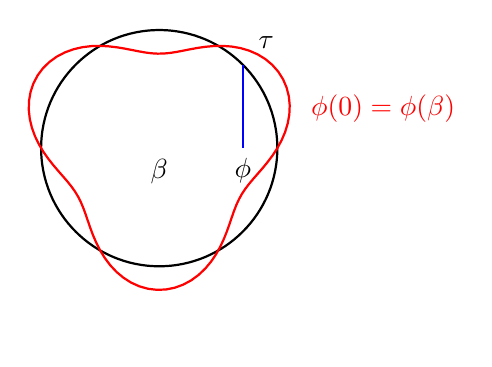
\begin{tikzpicture}[scale=1.0]
    % 虚时圆
    \draw[thick, ->] (0,0) circle (1.5);
    \node at (0,-0.3) {$\beta$};
    \draw[thick, blue] (45:1.5) -- (45:1.5 |- 0,0) node[below, black] {$\phi$};
    \node[above right] at (45:1.6) {$\tau$};
    % 周期性路径
    \draw[thick, red, domain=0:360, samples=100] plot ({1.5*cos(\x) + 0.3*sin(3*\x)*cos(\x)}, {1.5*sin(\x) + 0.3*sin(3*\x)*sin(\x)});
    \node[right, red] at (1.8,0.5) {$\phi(0)=\phi(\beta)$};
    % 标注
    \node at (0,-2.3) {虚时方向上的周期性场构型};
\end{tikzpicture}
\caption{配分函数路径积分中的周期性边界条件示意图。虚时方向形成一个周长为 $\beta = 1/(k_BT)$ 的圆，场构型在此方向上必须满足周期性条件 $\phi(0) = \phi(\beta)$。}
\label{fig:periodic}
\end{figure}

路径积分表述告诉我们，量子统计力学等价于一个在虚时方向上具有周期性边界条件的经典场论。虚时方向的长度 $\beta = 1/(k_B T)$ 与温度成反比。温度越高，虚时方向越短；温度越低，虚时方向越长。

\section{相图与临界现象}

统计力学的一个重要应用是描述物质的相变行为\cite{Landau1937}。图 \ref{fig:phase_diagram} 展示了典型的物质相图。

\begin{figure}[htbp]
\centering
\begin{tikzpicture}[scale=1.2]
    % 坐标轴
    \draw[thick, ->] (0,0) -- (4.5,0) node[right] {$T$};
    \draw[thick, ->] (0,0) -- (0,4.5) node[above] {$P$};
    % 相界线
    \draw[thick, red, domain=0.5:3.5, samples=50] plot (\x, {3.5/(\x+0.2)-0.5}) node[right] {气液相界};
    \draw[thick, blue] (1.5,0) -- (1.5,3.5) node[above] {固液相界};
    % 区域标注
    \node at (0.8,1) {固};
    \node at (2.5,0.8) {液};
    \node at (3.5,1.5) {气};
    % 关键点
    \fill[red] (1.5,2.8) circle (2pt) node[above right] {三相点};
    \fill[blue] (3.0,2.2) circle (2pt) node[above right] {临界点};
    % 临界点标注
    \draw[thick, dashed] (3.0,0) -- (3.0,2.2);
    \node[below] at (3.0,0) {$T_c$};
    % 临界指数标注
    \draw[<->, thick] (3.0,2.5) -- (3.8,2.5) node[right] {$|T-T_c|^{-\nu}$};
\end{tikzpicture}
\caption{典型的物质相图（$P$-$T$ 图）。气液相界线在临界点 $(T_c, P_c)$ 终结，此处相变变为连续的。在临界点附近，关联长度趋于无穷，系统表现出标度不变性和普适性\cite{Wilson1974}。}
\label{fig:phase_diagram}
\end{figure}

\begin{remark}[配分函数与相变]
相变对应于配分函数（或其导数）的奇异性。对于有限系统，配分函数是解析函数，不存在真正的相变。只有在热力学极限下，$\ln Z$ 的奇异性才可能出现。Lee-Yang 定理严格证明了这一点：相变来自配分函数零点在复平面上逼近实轴。
\end{remark}

\begin{remark}[临界指数与普适性]
在临界点附近，热力学量表现出幂律行为，例如比热容 $C \sim |T - T_c|^{-\alpha}$、序参量 $\phi \sim |T - T_c|^{\beta}$、关联长度 $\xi \sim |T - T_c|^{-\nu}$ 等。令人惊奇的是，临界指数 $\alpha, \beta, \nu, \ldots$ 仅依赖于系统的对称性和空间维度，而与微观细节无关。这一\textbf{普适性}（universality）由重正化群理论给出了解释\cite{Wilson1974}：不同微观系统在重正化群流下流向相同的不动点，因此表现出相同的临界行为。
\end{remark}

\begin{remark}[全息原理与配分函数]
在 AdS/CFT 对偶\cite{Maldacena1997}中，边界共形场论（CFT）的配分函数等于体引力理论的配分函数：
\begin{equation}
    Z_{\text{CFT}} = Z_{\text{gravity}}.
\end{equation}
这就是 GKPW（Gubser-Klebanov-Polyakov-Witten）关系。具体地，如果 CFT 中某个算符 $\mathcal{O}$ 的源为 $\phi_0$，则：
\begin{equation}
    Z_{\text{CFT}}[\phi_0] = \left. Z_{\text{gravity}}[\phi]
\right|_{\phi \to \phi_0 \text{ at boundary}},
\end{equation}
即引力侧的路径积分在边界上取值为 CFT 的源。

特别地，对于有限温度的 CFT，其配分函数对应于 AdS 空间中的黑洞背景\cite{Hawking1983}。黑洞的霍金温度恰好等于 CFT 的温度，黑洞的贝肯斯坦-霍金熵等于 CFT 的热力学熵。这个对偶是理解量子引力和强耦合场论的最有力工具之一。
\end{remark}

\begin{example}[Schwarzschild-AdS 黑洞与 CFT 热力学]
考虑 AdS$_5$ 中的 Schwarzschild 黑洞，其视界半径 $r_h$ 与边界 CFT 的温度之间的关系为 $T = r_h/(\pi L^2)$，其中 $L$ 是 AdS 半径。黑洞的贝肯斯坦-霍金熵为：
\begin{equation}
    S_{\text{BH}} = \frac{\text{Area}}{4G_5} = \frac{\pi^2}{2G_5} V_3 r_h^3,
\end{equation}
其中 $V_3$ 是边界空间的体积。通过 AdS/CFT 对偶，这等于边界 $\mathcal{N}=4$ 超对称 Yang-Mills 理论在强耦合极限下的热力学熵。这验证了全息原理中配分函数相等的深刻含义。
\end{example}

\begin{note}[路径积分在量子场论中的推广]
在量子场论中，配分函数的路径积分表示推广为对所有场构型的泛函积分。对于标量场 $\phi(x)$：
\begin{equation}
    Z[J] = \int \mathcal{D}\phi \, \exp\left(-S_E[\phi] + \int d^dx \, J(x)\phi(x)\right),
\end{equation}
其中 $J(x)$ 是外源场。$Z[J]$ 是量子场论的生成泛函（generating functional），所有关联函数都可以通过对 $J$ 求泛函导数得到。在 AdS/CFT 中，这个生成泛函的对偶引力描述由 GKPW 规则给出\cite{Maldacena1997}。
\end{note}

\section{小结}

在本节中，我们介绍了配分函数在统计物理中的核心地位：
\begin{itemize}
    \item 统计力学是连接微观物理学和宏观热力学的桥梁
    \item 统计系综是描述系统概率分布的数学框架，包括微正则系综、正则系综和巨正则系综
    \item 经典配分函数是相空间上的积分，包含了所有热力学信息
    \item 量子配分函数是玻尔兹曼算符的迹
    \item 涨落理论将宏观响应函数与微观涨落联系起来，在相变附近涨落变得重要\cite{Landau1937}
    \item 路径积分表述将配分函数写成对所有场构型的积分，通过 Wick 转动连接了量子力学和统计力学
    \item 在 AdS/CFT 对偶中，配分函数是连接边界场论与体引力理论的核心对象\cite{Maldacena1997}
\end{itemize}
配分函数之所以如此重要，是因为它是一个"生成函数"：通过对它进行适当的微分运算，我们可以得到所有感兴趣的物理量。在下一节中，我们将看到配分函数在量子场论中扮演着类似的角色。

\begin{note}[配分函数的统一视角]
从更抽象的角度看，配分函数是一个关于外源 $J$ 的泛函 $Z[J]$：
\begin{itemize}
    \item 在统计力学中，$J = \beta$（逆温度），$Z[\beta] = \Tr e^{-\beta\hat{H}}$
    \item 在量子场论中，$J$ 是外源场，$Z[J] = \int \mathcal{D}\phi \, e^{-S[\phi] + J\cdot\phi}$
    \item 在 AdS/CFT 中，$J$ 是边界上算符的源，$Z_{\text{CFT}}[J] = Z_{\text{gravity}}[\phi_0 = J]$
\end{itemize}
这三种情况的共同结构是：配分函数编码了系统对外部扰动的全部线性和非线性响应信息。所有关联函数、响应函数和热力学量都可以通过对 $J$ 的泛函微分得到。这种统一视角是理解量子场论、统计物理和量子引力之间深层联系的关键。
\end{note}

%=============================================================================


\chapter{量子场论中的配分函数 (Partition Functions in Quantum Field Theory)}

%=============================================================================

量子场论（quantum field theory, QFT）是描述粒子物理和凝聚态物理的基本理论框架。在量子场论中，配分函数扮演着与统计物理中类似的核心角色，但它的物理意义更加丰富。它不仅是统计权重的总和，更是所有关联函数（correlation function）的生成泛函（generating functional）。在本节中，我们将介绍量子场论的基本概念，然后详细讨论配分函数的定义和性质。

\section{量子场论的基本概念}

\subsection{从粒子到场}

在经典力学中，我们用粒子的坐标 $q_i(t)$ 来描述系统。在量子力学中，我们将坐标提升为算符 $\hat{q}_i$。但在量子场论中，我们走得更远：基本对象不是粒子，而是\textbf{场}（field）$\phi(x)$，它是时空坐标 $x^\mu = (t, \vec{x})$ 的函数。

\begin{note}[为什么要用场？]
为什么我们需要场，而不是直接用粒子？有以下几个原因：
\begin{itemize}
    \item \textbf{狭义相对论的要求}：在狭义相对论中，信息传播不能超光速。如果我们用粒子描述，粒子之间的瞬时相互作用会违反因果性。场论通过局域相互作用解决了这个问题。
    \item \textbf{粒子数不守恒}：在相对论性理论中，粒子可以产生和湮灭（如正负电子对产生）。场论自然地描述了这种现象。
    \item \textbf{全同粒子}：场论自动处理了全同粒子的统计性质（玻色子或费米子）。
\end{itemize}
\end{note}

场可以是：
\begin{itemize}
    \item \textbf{标量场}（scalar field）：在洛伦兹变换下不变的场，如 Higgs 场。用一个实数或复数函数描述。
    \item \textbf{旋量场}（spinor field）：在洛伦兹变换下按旋量表示变换的场，如电子场。用四分量旋量描述。
    \item \textbf{矢量场}（vector field）：在洛伦兹变换下按矢量表示变换的场，如光子场。用四矢量描述。
\end{itemize}

\begin{figure}[htbp]
\centering
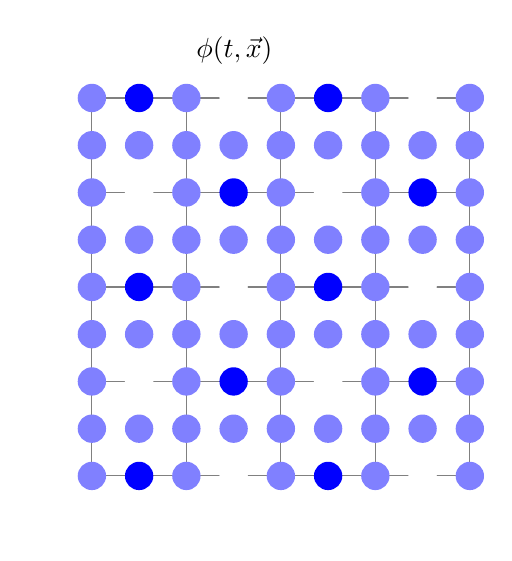
\begin{tikzpicture}[scale=1.2]
    % 绘制时空网格
    \draw[gray, thin] (0,0) grid (4,4);
    
    % 绘制场的值
    \foreach \x in {0,0.5,...,4} {
        \foreach \y in {0,0.5,...,4} {
            \pgfmathsetmacro{\val}{sin(\x*180)*cos(\y*180)}
            \pgfmathsetmacro{\colorval}{50+50*\val}
            \fill[blue!\colorval] (\x,\y) circle (0.15);
        }
    }
    
    % 标注
    \node at (2,-0.5) {空间};
    \node at (-0.5,2) {时间};
    \node at (2,4.5) {$\phi(t, \vec{x})$：场在每个时空点有一个值};
\end{tikzpicture}
\caption{场的直观理解。场 $\phi(t, \vec{x})$ 在每个时空点都有一个值，就像一张"橡皮膜"覆盖在整个时空上。}
\label{fig:field}
\end{figure}

\subsection{场算符与量子化}

在量子场论中，场被提升为算符 $\hat{\phi}(x)$，它作用在希尔伯特空间上。场算符满足对易关系（对于玻色子）或反对易关系（对于费米子）：
\begin{align}
    [\hat{\phi}(x), \hat{\pi}(y)] &= i\delta^{(3)}(\vec{x} - \vec{y}), \\
    \{\hat{\psi}(x), \hat{\psi}^\dagger(y)\} &= \delta^{(3)}(\vec{x} - \vec{y}),
\end{align}
其中 $\hat{\pi}$ 是共轭动量，$\hat{\psi}$ 是费米子场。

\begin{note}[量子化的物理意义]
量子化将经典场提升为算符，这带来了深刻的物理后果：
\begin{itemize}
    \item \textbf{真空涨落}：即使在真空中，场也在不断涨落。这些涨落导致了 Lamb 移位、Casimir 效应等可观测效应。
    \item \textbf{粒子产生}：场的量子涨落可以产生粒子-反粒子对。
    \item \textbf{不确定性原理}：场和共轭动量不能同时精确测量。
\end{itemize}
\end{note}

\subsection{真空态与粒子态}

\textbf{真空态}（vacuum state）$|0\rangle$：是系统的基态，即能量最低的状态。真空态满足 $\hat{H}|0\rangle = E_0|0\rangle$，其中 $E_0$ 是真空能量。

\begin{note}[真空不是"空"的]
在量子场论中，真空不是"空"的，而是充满了量子涨落。这些涨落导致了许多可观测效应：
\begin{itemize}
    \item \textbf{Lamb 移位}：氢原子能级的微小偏移，由真空涨落引起
    \item \textbf{Casimir 效应}：两块平行金属板之间的吸引力，由真空涨落引起
    \item \textbf{自发辐射}：激发态原子自发地发射光子，由真空涨落引起
\end{itemize}
\end{note}

\textbf{粒子态}（particle states）：通过对场算符作用在真空态上产生。例如，单粒子态为 $|p\rangle = \hat{a}^\dagger(p)|0\rangle$，其中 $\hat{a}^\dagger(p)$ 是产生算符。产生算符和湮灭算符满足对易关系：
\begin{equation}
    [\hat{a}(p), \hat{a}^\dagger(q)] = (2\pi)^3 2E_p \delta^{(3)}(\vec{p} - \vec{q}).
\end{equation}

\subsection{作用量与运动方程}

\textbf{拉格朗日密度}（Lagrangian density）$\mathcal{L}$：是场和场导数的函数，它决定了系统的动力学。拉格朗日密度必须是洛伦兹标量，并且满足局域性和幺正性。

\textbf{作用量}（action）$S[\phi]$：是场的泛函，定义为拉格朗日密度对时空的积分：
\begin{equation}
    S[\phi] = \int d^d x \, \mathcal{L}(\phi, \partial_\mu \phi).
\end{equation}

\begin{note}[最小作用量原理]
根据最小作用量原理，经典运动方程由作用量的极值条件给出：
\begin{equation}
    \frac{\delta S}{\delta \phi(x)} = 0.
\end{equation}
这个原理将物理学中的所有动力学统一在一个框架下：粒子沿着使作用量极值的路径运动，场沿着使作用量极值的构型演化。
\end{note}

\begin{example}[标量场的 Klein-Gordon 作用量]
考虑标量场 $\phi$，作用量为：
\begin{equation}
    S[\phi] = \int d^d x \left[ \frac{1}{2}(\partial_\mu \phi)^2 - \frac{1}{2}m^2 \phi^2 - V(\phi) \right],
\end{equation}
其中 $m$ 是质量，$V(\phi)$ 是相互作用势。第一项是动能项，第二项是质量项，第三项是相互作用项。

运动方程为 $(\Box + m^2)\phi = 0$，其中 $\Box = \partial_\mu \partial^\mu$ 是达朗贝尔算符。这个方程描述了自由标量场的传播。
\end{example}

\section{路径积分量子化}

\subsection{从经典到量子}

在经典力学中，粒子沿着使作用量极值的路径运动。在量子力学中，粒子可以沿着所有可能的路径运动，每条路径贡献一个相位 $e^{iS/\hbar}$。这就是费曼的路径积分表述。

\begin{note}[路径积分的物理直觉]
路径积分的核心思想是：量子理论是对所有可能历史的求和。这类似于统计力学中的配分函数——在统计力学中，我们对所有可能的微观状态求和；在量子力学中，我们对所有可能的路径求和。

这个思想的深刻之处在于：它将量子力学的叠加原理推广到了路径空间。在量子力学中，一个粒子可以同时处于多个位置；在路径积分中，一个粒子可以同时沿着多条路径运动。
\end{note}

\begin{figure}[htbp]
\centering
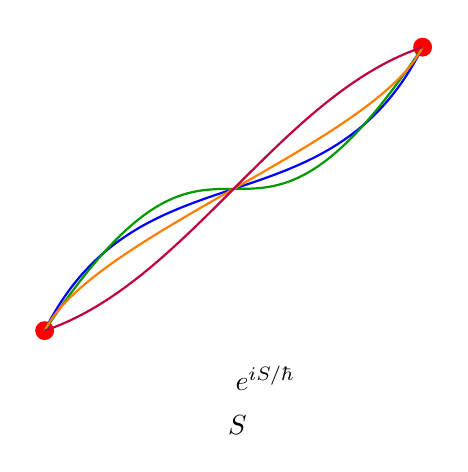
\begin{tikzpicture}[scale=1.2]
    % 绘制起点和终点
    \fill[red] (0,0) circle (0.1) node[below] {起点};
    \fill[red] (4,3) circle (0.1) node[above] {终点};
    
    % 绘制多条路径
    \draw[blue, thick] (0,0) .. controls (1,2) and (3,1) .. (4,3);
    \draw[green!60!black, thick] (0,0) .. controls (2,3) and (2,0) .. (4,3);
    \draw[orange, thick] (0,0) .. controls (0.5,1) and (3.5,2) .. (4,3);
    \draw[purple, thick] (0,0) .. controls (1.5,0.5) and (2.5,2.5) .. (4,3);
    
    % 标注
    \node at (2,-0.5) {所有路径都贡献 $e^{iS/\hbar}$};
    \node at (2,-1) {经典路径是使 $S$ 极值的路径};
\end{tikzpicture}
\caption{路径积分的直观理解。粒子从起点到终点，可以沿着所有可能的路径运动。每条路径贡献一个相位 $e^{iS/\hbar}$，经典路径是使作用量 $S$ 极值的路径。}
\label{fig:path_integral}
\end{figure}

\subsection{配分函数（生成泛函）}

\begin{definition}[配分函数]
\textbf{配分函数}（partition function）$Z[J]$ 定义为：
\begin{equation}
    Z[J] = \int \mathcal{D}\phi \, e^{-S[\phi] + \int d^d x \, J(x) \phi(x)},
    \label{eq:QFT_Z}
\end{equation}
其中：
\begin{itemize}
    \item $\mathcal{D}\phi$ 是路径积分测度，表示对所有可能的场构型求和
    \item $S[\phi]$ 是作用量
    \item $J(x)$ 是外源，是一个辅助场，我们加上它是为了能够通过微分来生成关联函数
\end{itemize}
\end{definition}

\begin{note}[配分函数的物理意义]
配分函数 $Z[J]$ 是量子场论中最核心的对象。它的物理意义是：
\begin{itemize}
    \item \textbf{生成泛函}：通过对外源 $J$ 求泛函微分，可以得到所有关联函数。这使得配分函数成为"生成"所有物理量的"母函数"。
    \item \textbf{路径积分}：配分函数是对所有可能场构型的加权求和，权重是 $e^{-S}$。这类似于统计力学中的配分函数。
    \item \textbf{与 AdS/CFT 的联系}：在 AdS/CFT 对偶中，CFT 的配分函数等于引力理论的配分函数：$Z_{\rm CFT} = Z_{\rm gravity}$。
\end{itemize}
\end{note}

\subsection{路径积分测度}

\textbf{路径积分测度}的定义：将时空离散化为 $N$ 个点，对每个点的场值积分，然后取 $N \to \infty$ 的极限：
\begin{equation}
    \int \mathcal{D}\phi = \lim_{N \to \infty} \prod_{i=1}^{N} \int d\phi(x_i).
\end{equation}
这个定义虽然形式上简单，但在实际计算中通常需要正规化（regularization）。

\subsection{欧几里得配分函数}

\textbf{欧几里得配分函数}：在欧几里得空间中，配分函数定义为：
\begin{equation}
    Z_E[J] = \int \mathcal{D}\phi \, e^{-S_E[\phi] + \int d^d x \, J(x) \phi(x)},
\end{equation}
其中 $S_E[\phi]$ 是欧几里得作用量，它是通过 Wick 转动 $t \to -i\tau$ 从闵可夫斯基作用量得到的。

\begin{note}[为什么要 Wick 转动？]
Wick 转动将闵可夫斯基空间变为欧几里得空间，这有几个好处：
\begin{itemize}
    \item \textbf{收敛性}：在闵可夫斯基空间中，被积函数是振荡的 $e^{iS}$，积分不收敛；在欧几里得空间中，被积函数是衰减的 $e^{-S_E}$，积分良定义。
    \item \textbf{与统计力学的联系}：欧几里得路径积分与统计力学的配分函数形式相同，这揭示了量子场论与统计力学之间的深刻联系。
    \item \textbf{数值计算}：欧几里得路径积分更容易用数值方法（如格点 QCD）计算。
\end{itemize}
\end{note}

\section{关联函数}

\subsection{关联函数的定义}

关联函数是量子场论中最重要的物理量之一，它描述了场在不同时空点的关联程度。关联函数可以直接与实验测量相联系——散射截面、衰变率等所有可观测量都可以用关联函数表示。

\begin{theorem}[$n$ 点关联函数]
\textbf{$n$ 点关联函数}定义为：
\begin{equation}
    \langle \phi(x_1) \cdots \phi(x_n) \rangle = \frac{1}{Z[0]} \int \mathcal{D}\phi \, \phi(x_1) \cdots \phi(x_n) \, e^{-S[\phi]}.
\end{equation}
这个定义表明，关联函数是场算符在路径积分下的期望值。
\end{theorem}

关联函数可以通过对配分函数进行 $n$ 次泛函微分得到：
\begin{equation}
    \langle \phi(x_1) \cdots \phi(x_n) \rangle = \frac{1}{Z[0]} \left. \frac{\delta^n Z[J]}{\delta J(x_1) \cdots \delta J(x_n)} \right|_{J=0}.
    \label{eq:QFT_corr}
\end{equation}
这个公式表明，配分函数包含了所有关联函数的信息。

\begin{note}[关联函数的物理意义]
关联函数描述了场在不同时空点的关联程度：
\begin{itemize}
    \item \textbf{两点函数} $\langle \phi(x) \phi(y) \rangle$：描述了粒子从 $y$ 传播到 $x$ 的振幅
    \item \textbf{三点函数} $\langle \phi(x) \phi(y) \phi(z) \rangle$：描述了三个粒子之间的相互作用
    \item \textbf{$n$ 点函数}：描述了 $n$ 个粒子之间的关联
\end{itemize}
所有可观测量（如散射截面、衰变率）都可以用关联函数表示。
\end{note}

\subsection{传播子}

\begin{definition}[传播子]
\textbf{传播子}（propagator）：自由场的两点关联函数称为传播子：
\begin{equation}
    \langle \phi(x) \phi(y) \rangle_0 = \int \frac{d^d k}{(2\pi)^d} \frac{e^{ik \cdot (x-y)}}{k^2 + m^2}.
\end{equation}
传播子描述了粒子从 $y$ 传播到 $x$ 的振幅。在动量空间中，传播子为 $1/(k^2 + m^2)$，这是 Klein-Gordon 算符的逆。
\end{definition}

\begin{note}[传播子的物理图像]
传播子可以被理解为粒子在时空中传播的"概率幅"。当粒子从 $y$ 传播到 $x$ 时，它会经历所有可能的路径，每条路径贡献一个相位。传播子就是这些路径的相干叠加。

在动量空间中，传播子 $1/(k^2 + m^2)$ 有一个极点在 $k^2 = -m^2$ 处，这对应于质壳条件（on-shell condition）。物理上，这意味着传播子主要由质壳上的粒子贡献。
\end{note}

\section{连通关联函数和 1PI 关联函数}

\subsection{连通关联函数}

关联函数可以分解为连通部分和非连通部分。这种分解在微扰计算中非常重要。

\begin{definition}[连通关联函数]
\textbf{连通生成泛函}（connected generating functional）$W[J]$ 定义为：
\begin{equation}
    W[J] = \ln Z[J].
\end{equation}
连通关联函数通过 $W[J]$ 的泛函微分得到：
\begin{equation}
    \langle \phi(x_1) \cdots \phi(x_n) \rangle_{\rm conn} = \left. \frac{\delta^n W[J]}{\delta J(x_1) \cdots \delta J(x_n)} \right|_{J=0}.
\end{equation}
\end{definition}

\begin{note}[连通与非连通的区别]
连通关联函数只包含"真正"的关联，不包含由于独立部分的关联导致的"假"关联。例如，对于两点函数：
\begin{equation}
    \langle \phi(x) \phi(y) \rangle = \langle \phi(x) \phi(y) \rangle_{\rm conn} + \langle \phi(x) \rangle \langle \phi(y) \rangle.
\end{equation}
第一项是连通部分，描述了 $x$ 和 $y$ 之间的真实关联；第二项是非连通部分，是两个独立期望值的乘积。
\end{note}

\subsection{1PI 关联函数}

\begin{definition}[1PI 关联函数]
\textbf{单粒子不可约}（one-particle irreducible, 1PI）关联函数：是不能通过切断一条内线而分成两部分的费曼图的贡献。1PI 关联函数在量子场论中起着核心作用，因为它们包含了所有量子修正的信息。
\end{definition}

\begin{note}[1PI 的物理意义]
1PI 图是量子场论中"不可约"的相互作用。例如，在 $\phi^4$ 理论中，单圈 1PI 图是一个"气泡"，它不能被分解为更简单的图。1PI 图包含了所有量子修正的信息，是计算有效作用量的基础。
\end{note}

\section{有效作用量}

\subsection{有效作用量的定义}

\begin{definition}[有效作用量]
有效作用量（effective action）$\Gamma[\phi_{\rm cl}]$ 是量子场论中另一个重要的概念。它是通过对 $W[J]$ 进行勒让德变换得到的：
\begin{equation}
    \Gamma[\phi_{\rm cl}] = W[J] - \int d^d x \, J(x) \phi_{\rm cl}(x),
    \label{eq:eff_action}
\end{equation}
其中 $\phi_{\rm cl}(x) = \delta W / \delta J(x)$ 是经典场，即场算符的真空期望值：
\begin{equation}
    \phi_{\rm cl}(x) = \langle \hat{\phi}(x) \rangle_J.
\end{equation}
\end{definition}

\begin{note}[有效作用量的物理意义]
有效作用量是量子场论中最重要的概念之一。它的物理意义是：
\begin{itemize}
    \item \textbf{包含所有量子修正}：有效作用量包含了所有圈图（量子修正）的贡献。经典作用量只包含树图（经典）贡献。
    \item \textbf{量子运动方程}：有效作用量的运动方程 $\delta \Gamma / \delta \phi_{\rm cl} = -J$ 给出量子理论的真空态。当 $J = 0$ 时，这给出了量子修正的真空。
    \item \textbf{1PI 生成泛函}：有效作用量是 1PI 关联函数的生成泛函。
\end{itemize}
\end{note}

\subsection{有效作用量的性质}

\begin{property}[有效作用量的性质]
\textbf{有效作用量的性质}：
\begin{itemize}
    \item 有效作用量包含了所有量子修正（quantum correction）的贡献
    \item 有效作用量的运动方程 $\delta \Gamma / \delta \phi_{\rm cl} = -J$ 给出量子理论的真空态（当 $J = 0$ 时）
    \item 有效作用量的展开系数给出 1PI 关联函数
\end{itemize}
\end{property}

\subsection{树图与圈图}

\begin{remark}[树图与圈图]
\textbf{树图近似}（tree approximation）：在树图近似下，有效作用量等于经典作用量：$\Gamma[\phi_{\rm cl}] = S[\phi_{\rm cl}]$。树图对应于经典物理。

\textbf{圈图修正}（loop corrections）：量子修正以圈图的形式出现：
\begin{equation}
    \Gamma[\phi_{\rm cl}] = S[\phi_{\rm cl}] + \hbar \Gamma_1[\phi_{\rm cl}] + \hbar^2 \Gamma_2[\phi_{\rm cl}] + \cdots
\end{equation}
其中 $\Gamma_n$ 是 $n$ 圈图的贡献。圈图对应于量子效应。
\end{remark}

\section{费曼图}

\subsection{费曼图的物理直觉}

费曼图是计算关联函数的图形方法，由费曼于 1948 年提出。费曼图将复杂的数学表达式转化为直观的图形，极大地简化了微扰计算。

\begin{note}[费曼图的物理意义]
费曼图不仅仅是计算工具，它们还有深刻的物理意义：
\begin{itemize}
    \item \textbf{粒子的传播}：线代表粒子在时空中传播
    \item \textbf{相互作用}：顶点代表粒子之间的相互作用
    \item \textbf{量子涨落}：圈代表量子涨落（虚粒子的产生和湮灭）
\end{itemize}
费曼图将量子场论的计算转化为"粒子物理"的语言，使得物理直觉可以指导计算。
\end{note}

\section{费曼规则}

费曼规则是从路径积分形式体系中系统地推导出来的计算规则，它将关联函数的计算转化为代数运算。本节将从路径积分出发，详细推导费曼规则的每一个组成部分。

\begin{definition}[费曼规则]
\textbf{费曼规则}（Feynman rules）：将费曼图的每个元素映射到数学表达式的规则体系：
\begin{itemize}
    \item \textbf{外线}（external lines）：外态粒子的波函数（标量场取 1）
    \item \textbf{内线}（internal lines）：传播子 $\Delta(k) = 1/(k^2 + m^2)$
    \item \textbf{顶点}（vertices）：相互作用拉格朗日量中的耦合常数
    \item \textbf{圈}（loops）：对未确定动量的积分 $\int d^d k/(2\pi)^d$
    \item \textbf{对称性因子}（symmetry factor）：$1/S$，消除重复计数
\end{itemize}
\end{definition}

\begin{note}[费曼规则的物理来源]
费曼规则不是"人为规定"的，而是从路径积分严格推导出来的。推导的逻辑链条为：
\begin{enumerate}
    \item \textbf{配分函数的微扰展开}：将 $Z[J]$ 按耦合常数展开为无穷级数
    \item \textbf{高斯积分}：对自由场部分做高斯积分，产生传播子
    \item \textbf{Wick 定理}：将场算符的乘积分解为传播子的组合
    \item \textbf{图形表示}：将代数表达式用图形（费曼图）表示
\end{enumerate}
每条费曼规则都对应路径积分中的一个精确的数学步骤。
\end{note}

%------ 传播子的推导 ------

\subsection{传播子的推导}

\begin{theorem}[自由场传播子]
对于自由标量场，传播子是自由场的两点关联函数。考虑配分函数：
\begin{equation}
    Z_0[J] = \int \mathcal{D}\phi \, \exp\left\{-\int d^d x \left[\frac{1}{2}(\partial_\mu \phi)^2 + \frac{1}{2}m^2 \phi^2 - J\phi\right]\right\}.
\end{equation}
\end{theorem}

\begin{proof}[传播子的完整推导]
推导分为以下步骤：

\textbf{第一步：动量空间的作用量}

对场做傅里叶变换 $\phi(x) = \int \frac{d^d k}{(2\pi)^d} \tilde{\phi}(k) e^{ik\cdot x}$，作用量变为：
\begin{equation}
    S_0[\phi, J] = \int \frac{d^d k}{(2\pi)^d} \left[\frac{1}{2}\tilde{\phi}(-k)(k^2 + m^2)\tilde{\phi}(k) - \tilde{J}(-k)\tilde{\phi}(k)\right].
\end{equation}
这里利用了 $\int d^d x \, (\partial_\mu \phi)^2 = \int \frac{d^d k}{(2\pi)^d} k^2 |\tilde{\phi}(k)|^2$（分部积分）。

\textbf{第二步：完成平方}

定义 $A(k) = k^2 + m^2$，配方得：
\begin{equation}
    S_0 = \int \frac{d^d k}{(2\pi)^d} \frac{1}{2}A(k)\left[\tilde{\phi}(k) - \frac{\tilde{J}(k)}{A(k)}\right]\left[\tilde{\phi}(-k) - \frac{\tilde{J}(-k)}{A(k)}\right] - \frac{1}{2}\frac{\tilde{J}(k)\tilde{J}(-k)}{A(k)}.
\end{equation}

\textbf{第三步：做高斯积分}

对 $\tilde{\phi}$ 积分（高斯积分），得到：
\begin{equation}
    Z_0[J] = Z_0[0] \exp\left[\frac{1}{2}\int \frac{d^d k}{(2\pi)^d} \frac{\tilde{J}(k)\tilde{J}(-k)}{k^2 + m^2}\right].
\end{equation}

\textbf{第四步：对 $J$ 求泛函导数}

两点关联函数为：
\begin{equation}
    \langle \phi(x)\phi(y)\rangle = \frac{1}{Z_0[0]}\left.\frac{\delta^2 Z_0[J]}{\delta J(x)\delta J(y)}\right|_{J=0} = \int \frac{d^d k}{(2\pi)^d} \frac{e^{ik\cdot(x-y)}}{k^2 + m^2} \equiv \Delta(x-y).
\end{equation}
\end{proof}

\begin{figure}[htbp]
\centering
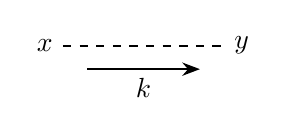
\begin{tikzpicture}
    \begin{feynman}
        \vertex (a) {$x$};
        \vertex[right=2.5cm of a] (b) {$y$};
        \diagram* {
            (a) -- [scalar, momentum'={$k$}] (b),
        };
    \end{feynman}
\end{tikzpicture}
\caption{自由标量场的传播子。在动量空间中，传播子为 $\Delta(k) = 1/(k^2 + m^2)$。}
\label{fig:propagator}
\end{figure}

\begin{remark}[传播子的物理意义]
传播子 $\Delta(k) = 1/(k^2 + m^2)$ 有深刻的物理含义：
\begin{itemize}
    \item \textbf{极点}：在 $k^2 = -m^2$ 处有极点，对应于质壳条件 $E^2 = \vec{p}^2 + m^2$
    \item \textbf{虚粒子}：不在质壳上的传播子描述了虚粒子（virtual particle）的传播
    \item \textbf{闵可夫斯基 vs 欧几里得}：闵可夫斯基空间传播子为 $i/(k^2 - m^2 + i\epsilon)$，欧几里得空间为 $1/(k^2 + m^2)$
\end{itemize}
$i\epsilon$ 项（Feynman prescription）确保了因果性：正频模向未来传播，负频模向过去传播。
\end{remark}

%------ 顶点因子的推导 ------

\subsection{顶点因子的推导}

\begin{theorem}[相互作用顶点]
顶点因子来自于相互作用项在微扰展开中的贡献。对于一般的相互作用 $\mathcal{L}_{\rm int} = -\frac{\lambda}{n!}\phi^n$，每个顶点贡献因子 $-\lambda$（欧几里得空间）或 $-i\lambda$（闵可夫斯基空间）。
\end{theorem}

\begin{proof}[$\phi^4$ 理论顶点的推导]
考虑 $\phi^4$ 相互作用：
\begin{equation}
    S_{\rm int} = \frac{\lambda}{4!}\int d^d x \, \phi(x)^4.
\end{equation}

将 $e^{-S_{\rm int}}$ 展开：
\begin{equation}
    e^{-S_{\rm int}} = 1 - \frac{\lambda}{4!}\int d^d x \, \phi(x)^4 + \frac{1}{2!}\left(\frac{\lambda}{4!}\right)^2 \int d^d x \, d^d y \, \phi(x)^4 \phi(y)^4 + \cdots
\end{equation}

一阶项 $-\frac{\lambda}{4!}\int d^d x \, \phi(x)^4$ 产生一个顶点。因子 $4!$ 来自于 $\phi^4$ 的排列组合数，在做 Wick 缩并时，每个顶点有 $4!$ 种配对方式，恰好与分母抵消。因此每个顶点净贡献因子 $-\lambda$。
\end{proof}

\begin{figure}[htbp]
\centering
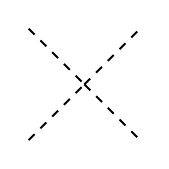
\begin{tikzpicture}
    \begin{feynman}
        \vertex (o);
        \vertex[above left=1cm of o] (a);
        \vertex[below left=1cm of o] (b);
        \vertex[above right=1cm of o] (c);
        \vertex[below right=1cm of o] (d);
        \diagram* {
            (a) -- [scalar] (o),
            (b) -- [scalar] (o),
            (o) -- [scalar] (c),
            (o) -- [scalar] (d),
        };
    \end{feynman}
\end{tikzpicture}
\caption{$\phi^4$ 理论的四点顶点。每个顶点贡献因子 $-\lambda$，有 4 条线连接。}
\label{fig:vertex}
\end{figure}

%------ 对称性因子 ------

\subsection{对称性因子}

\begin{definition}[对称性因子]
\textbf{对称性因子}（symmetry factor）$S$：一个费曼图内部对称变换的数目，用于消除 Wick 缩并中的重复计数。
\end{definition}

\begin{example}[对称性因子的计算]
考虑以下"浴缸图"（tadpole diagram）：
\begin{figure}[htbp]
\centering
\begin{tikzpicture}
    \begin{feynman}
        \vertex (a);
        \vertex[right=2cm of a] (b);
        \diagram* {
            (a) -- [scalar] (b),
            (b) -- [scalar, half right, looseness=2] (b),
        };
    \end{feynman}
\end{tikzpicture}
\caption{浴缸图（tadpole）。圈可以沿任何方向遍历，产生因子 $S=2$。}
\label{fig:tadpole}
\end{figure}

对称性因子为 $S=2$（圈的两条线可以交换）。因此贡献为 $-\lambda/2 \cdot \int d^d k/(2\pi)^d \cdot 1/(k^2+m^2)$。
\end{example}

\begin{property}[对称性因子的计算规则]
对称性因子可以通过以下方式计算：
\begin{enumerate}
    \item 数出可以交换的等价线的数目
    \item 数出可以交换的等价顶点的数目
    \item 数出可以翻转的圈的数目
\end{enumerate}
对于 $\phi^4$ 理论，常见的对称性因子有：
\begin{itemize}
    \item 自能图（"太阳图"）：$S = 2$
    \item 浴缸图（tadpole）：$S = 2$
    \item "眼镜图"（s, t, u 通道）：$S = 2$
\end{itemize}
\end{property}

%------ 完整的费曼规则汇总 ------

\subsection{费曼规则的完整汇总}

\begin{theorem}[$\phi^4$ 理论的完整费曼规则]
对于欧几里得空间中的 $\phi^4$ 理论 $\mathcal{L} = \frac{1}{2}(\partial\phi)^2 + \frac{1}{2}m^2\phi^2 + \frac{\lambda}{4!}\phi^4$，费曼规则为：
\begin{enumerate}
    \item \textbf{传播子}：$\displaystyle \frac{1}{k^2 + m^2}$\quad（内部线，用直线表示）
    \item \textbf{顶点因子}：$-\lambda$\quad（4 条线的交点）
    \item \textbf{外线因子}：$1$\quad（标量场的外线）
    \item \textbf{圈积分}：$\displaystyle \int \frac{d^d k}{(2\pi)^d}$\quad（每个未确定的内部动量）
    \item \textbf{动量守恒}：每个顶点处 $\sum k_{\rm in} = \sum k_{\rm out}$
    \item \textbf{对称性因子}：$1/S$
\end{enumerate}

对于闵可夫斯基空间，将传播子替换为 $i/(k^2 - m^2 + i\epsilon)$，顶点替换为 $-i\lambda$。
\end{theorem}

\begin{remark}[Wick 定理与费曼规则的关系]
费曼规则的本质是 \textbf{Wick 定理}：将时间编序的场算符乘积分解为传播子的组合。
\begin{equation}
    T\{\phi(x_1)\cdots\phi(x_n)\} = :\!\phi(x_1)\cdots\phi(x_n)\!: + \text{所有可能的缩并},
\end{equation}
其中 $:\cdots:$ 表示正规序（normal ordering），缩并 $\phi(x)\phi(y)$ 就是传播子 $\Delta(x-y)$。
每个费曼图对应 Wick 定理中的一种缩并方式。
\end{remark}

\section{$\phi^4$ 理论：完整计算示例}

$\phi^4$ 理论是量子场论中最简单的可重正化相互作用理论，虽然它不描述真实粒子物理（标量 $\phi^4$ 理论在 4 维是"平庸的"），但它是学习费曼图计算、正规化和重整化的最佳范例。本节将用 $\phi^4$ 理论作为"量子场论的实验室"，完整演示从拉格朗日量到物理可观测量的计算流程。

\begin{definition}[$\phi^4$ 理论]
\textbf{$\phi^4$ 理论}的拉格朗日密度为：
\begin{equation}
    \mathcal{L} = \frac{1}{2}(\partial_\mu \phi)^2 - \frac{1}{2}m^2 \phi^2 - \frac{\lambda}{4!} \phi^4.
\end{equation}
其中 $m$ 是粒子质量，$\lambda$ 是无量纲耦合常数（在 4 维中）。因子 $4!$ 是为了消除 Wick 缩并中的重复计数而引入的约定。
\end{definition}

\begin{property}[$\phi^4$ 理论的费曼规则]
在欧几里得空间中，$\phi^4$ 理论的费曼规则为：
\begin{enumerate}
    \item \textbf{传播子}：$\displaystyle \Delta(k) = \frac{1}{k^2 + m^2}$
    \item \textbf{顶点因子}：$-\lambda$
    \item \textbf{外线因子}：$1$（标量场）
    \item \textbf{圈积分}：$\displaystyle \int \frac{d^d k}{(2\pi)^d}$
    \item \textbf{动量守恒}：每个顶点处四条线的动量之和为零
\end{enumerate}
\end{property}

%------ 两点函数 ------

\subsection{两点函数的逐阶计算}

两点函数（传播子的全量子修正）是理解自能、质量重整化的最简单例子。我们按 $\lambda$ 的幂次逐阶计算。

\begin{example}[两点函数的树图贡献（$\lambda^0$ 阶）]
在树图水平，两点函数就是自由场传播子：
\begin{equation}
    G^{(2)}_{\rm tree}(p) = \frac{1}{p^2 + m^2}.
\end{equation}
\begin{figure}[htbp]
\centering
\begin{tikzpicture}
    \begin{feynman}
        \vertex (a) {$x$};
        \vertex[right=2.5cm of a] (b) {$y$};
        \diagram* {
            (a) -- [scalar] (b),
        };
    \end{feynman}
\end{tikzpicture}
\caption{两点函数的树图贡献：自由传播子。}
\label{fig:phi4_2pt_tree}
\end{figure}
\end{example}

\begin{example}[两点函数的单圈修正（$\lambda^1$ 阶）]
在 $\lambda^1$ 阶，两点函数有一个单圈修正——"自能图"（self-energy diagram），也称为"太阳图"（sunset diagram，不过这里其实是"哑铃图"）：
\begin{figure}[htbp]
\centering
\begin{tikzpicture}
    \begin{feynman}
        \vertex (a);
        \vertex[right=1.5cm of a] (b);
        \vertex[right=1.5cm of b] (c);
        \vertex[right=1.5cm of c] (d);
        \diagram* {
            (a) -- [scalar] (b),
            (b) -- [scalar, half left, looseness=1.5] (c),
            (b) -- [scalar, half right, looseness=1.5] (c),
            (c) -- [scalar] (d),
        };
    \end{feynman}
\end{tikzpicture}
\caption{$\phi^4$ 理论中两点函数的单圈修正（自能图）。}
\label{fig:phi4_self_energy}
\end{figure}

\textbf{详细计算}：自能 $\Sigma(p)$ 的贡献为：
\begin{equation}
    \Sigma(p) = \frac{\lambda}{2} \int \frac{d^d k}{(2\pi)^d} \frac{1}{k^2 + m^2},
\end{equation}

推导过程：
\begin{enumerate}
    \item 一个顶点贡献因子 $-\lambda$
    \item 两条内部线各贡献传播子 $1/(k^2 + m^2)$，但这里只有一条内部线形成圈
    \item 对称性因子 $S = 2$（圈中两条线可交换），因此 $1/S = 1/2$
    \item 对圈动量 $k$ 积分
\end{enumerate}

\textbf{注意}：这个积分在 $k \to \infty$ 时发散（紫外发散）！在 $d = 4$ 维中，
\begin{equation}
    \Sigma \sim \frac{\lambda}{2} \int_0^\Lambda \frac{k^3 dk}{k^2 + m^2} \sim \frac{\lambda}{2} \Lambda^2 \quad (\Lambda \to \infty).
\end{equation}
这表明我们需要正规化来处理这个发散。
\end{example}

\begin{remark}[戴森方程]
自能修正可以通过 \textbf{戴森方程}（Dyson equation）重新求和。全传播子为：
\begin{equation}
    G^{(2)}(p) = \frac{1}{p^2 + m^2} + \frac{1}{p^2 + m^2}\Sigma(p)\frac{1}{p^2 + m^2} + \cdots = \frac{1}{p^2 + m^2 - \Sigma(p)}.
\end{equation}
这是几何级数的求和，物理上对应于将所有自能修正"插入"到传播子中。
\begin{figure}[htbp]
\centering
\begin{tikzpicture}
    \begin{feynman}
        \vertex (a);
        \vertex[right=0.8cm of a] (b);
        \vertex[right=0.4cm of b] (dots1) {$\cdots$};
        \vertex[right=0.4cm of dots1] (c);
        \vertex[right=0.8cm of c] (d);
        \diagram* {
            (a) -- [scalar] (b),
            (b) -- [scalar, half left, looseness=1.5] (c),
            (b) -- [scalar, half right, looseness=1.5] (c),
            (c) -- [scalar] (d),
        };
    \end{feynman}
\end{tikzpicture}
\caption{戴森方程的图形表示：将自能修正无穷求和。}
\label{fig:dyson}
\end{figure}
\end{remark}

%------ 四点函数 ------

\subsection{四点函数的逐阶计算}

四点函数描述了粒子之间的散射过程，是粒子物理中最基本的可观测量。

\begin{example}[四点函数的树图贡献（$\lambda^1$ 阶）]
在树图水平，四点函数来自于一个顶点：
\begin{figure}[htbp]
\centering
\begin{tikzpicture}
    \begin{feynman}
        \vertex (a1) {$p_1$};
        \vertex[above right=1.5cm of a1] (b);
        \vertex[below right=1.5cm of a1] (c);
        \vertex[right=1.5cm of b] (d1) {$p_3$};
        \vertex[right=1.5cm of c] (d2) {$p_4$};
        \vertex[left=1.5cm of a1] (e) {$p_2$};
        \diagram* {
            (a1) -- [scalar] (b),
            (e) -- [scalar] (b),
            (b) -- [scalar] (d1),
            (b) -- [scalar] (d2),
        };
    \end{feynman}
\end{tikzpicture}
\caption{$\phi^4$ 理论中四点函数的树图贡献。}
\label{fig:phi4_4point_tree}
\end{figure}

在动量空间中，四点函数为：
\begin{equation}
    G^{(4)}_{\rm tree}(p_1, p_2, p_3, p_4) = -\lambda \cdot (2\pi)^d \delta^{(d)}(p_1 + p_2 + p_3 + p_4).
\end{equation}
这个结果表明，在树图水平，四个粒子通过一个四点顶点相互作用。动量守恒由 $\delta$ 函数保证。
\end{example}

\begin{example}[四点函数的单圈修正（$\lambda^2$ 阶）]
在 $\lambda^2$ 阶，四点函数有三个单圈修正，分别对应于 \textbf{Mandelstam 变量}的三个通道：
\begin{itemize}
    \item $s$ 通道：$s = (p_1 + p_2)^2$，粒子 1 和 2 合并再分裂
    \item $t$ 通道：$t = (p_1 - p_3)^2$，粒子 1 和 3 交换
    \item $u$ 通道：$u = (p_1 - p_4)^2$，粒子 1 和 4 交换
\end{itemize}

\begin{figure}[htbp]
\centering
\begin{subfigure}[b]{0.3\textwidth}
\centering
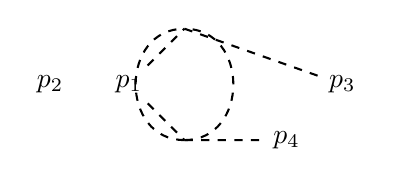
\begin{tikzpicture}[scale=0.8]
    \begin{feynman}
        \vertex (a1) {$p_1$};
        \vertex[below right=1cm of a1] (b);
        \vertex[above right=1cm of a1] (c);
        \vertex[below right=1cm of c] (d);
        \vertex[right=1cm of d] (e) {$p_3$};
        \vertex[right=1cm of b] (f) {$p_4$};
        \vertex[left=1cm of a1] (g) {$p_2$};
        \diagram* {
            (a1) -- [scalar] (b),
            (a1) -- [scalar] (c),
            (b) -- [scalar, half left, looseness=1.5] (c),
            (b) -- [scalar, half right, looseness=1.5] (c),
            (b) -- [scalar] (f),
            (c) -- [scalar] (e),
        };
    \end{feynman}
\end{tikzpicture}
\caption{$s$ 通道}
\end{subfigure}
\hfill
\begin{subfigure}[b]{0.3\textwidth}
\centering
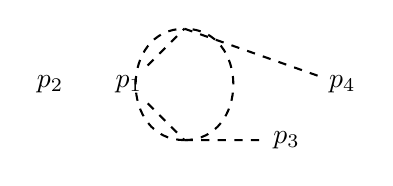
\begin{tikzpicture}[scale=0.8]
    \begin{feynman}
        \vertex (a1) {$p_1$};
        \vertex[below right=1cm of a1] (b);
        \vertex[above right=1cm of a1] (c);
        \vertex[below right=1cm of c] (d);
        \vertex[right=1cm of d] (e) {$p_4$};
        \vertex[right=1cm of b] (f) {$p_3$};
        \vertex[left=1cm of a1] (g) {$p_2$};
        \diagram* {
            (a1) -- [scalar] (b),
            (a1) -- [scalar] (c),
            (b) -- [scalar, half left, looseness=1.5] (c),
            (b) -- [scalar, half right, looseness=1.5] (c),
            (b) -- [scalar] (f),
            (c) -- [scalar] (e),
        };
    \end{feynman}
\end{tikzpicture}
\caption{$t$ 通道}
\end{subfigure}
\hfill
\begin{subfigure}[b]{0.3\textwidth}
\centering
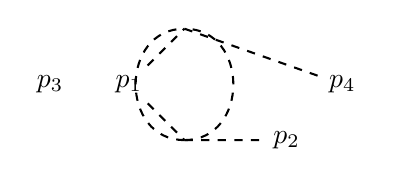
\begin{tikzpicture}[scale=0.8]
    \begin{feynman}
        \vertex (a1) {$p_1$};
        \vertex[below right=1cm of a1] (b);
        \vertex[above right=1cm of a1] (c);
        \vertex[below right=1cm of c] (d);
        \vertex[right=1cm of d] (e) {$p_4$};
        \vertex[right=1cm of b] (f) {$p_2$};
        \vertex[left=1cm of a1] (g) {$p_3$};
        \diagram* {
            (a1) -- [scalar] (b),
            (a1) -- [scalar] (c),
            (b) -- [scalar, half left, looseness=1.5] (c),
            (b) -- [scalar, half right, looseness=1.5] (c),
            (b) -- [scalar] (f),
            (c) -- [scalar] (e),
        };
    \end{feynman}
\end{tikzpicture}
\caption{$u$ 通道}
\end{subfigure}
\caption{$\phi^4$ 理论中四点函数的单圈修正。三个通道分别对应于不同的动量分配。}
\label{fig:phi4_4point_loop}
\end{figure}

每个通道的贡献为（以 $s$ 通道为例）：
\begin{equation}
    \mathcal{A}_s = \frac{\lambda^2}{2} \int \frac{d^d k}{(2\pi)^d} \frac{1}{k^2 + m^2} \frac{1}{(p_1 + p_2 - k)^2 + m^2},
\end{equation}

\textbf{详细计算步骤}：
\begin{enumerate}
    \item 两个顶点各贡献 $-\lambda$，总因子 $(-\lambda)^2 = \lambda^2$
    \item 两条内部传播子：$1/(k^2+m^2)$ 和 $1/((p_1+p_2-k)^2+m^2)$
    \item 对称性因子 $S = 2$，贡献 $1/2$
    \item 对圈动量 $k$ 积分，动量守恒约束了另一条内部线的动量
\end{enumerate}

总散射振幅为三个通道之和：
\begin{equation}
    \mathcal{A} = \mathcal{A}_s + \mathcal{A}_t + \mathcal{A}_u.
\end{equation}
\end{example}

\begin{remark}[Mandelstam 变量]
Mandelstam 变量 $s, t, u$ 是描述 $2 \to 2$ 散射的洛伦兹不变量：
\begin{equation}
    s = (p_1+p_2)^2, \quad t = (p_1-p_3)^2, \quad u = (p_1-p_4)^2,
\end{equation}
它们满足约束 $s + t + u = \sum_{i=1}^4 p_i^2 = 4m^2$（在质壳条件下）。
这三个变量分别对应于三个不同的物理过程：$s$ 通道是"合并-分裂"过程，$t$ 和 $u$ 通道是"交换"过程。
\end{remark}

%------ 发散与重整化 ------

\subsection{$\phi^4$ 理论中的发散与重整化}

\begin{note}[发散的物理意义]
在 $\phi^4$ 理论中，我们遇到了两类紫外发散：
\begin{itemize}
    \item \textbf{两点函数的发散}（自能发散 $\Sigma$）：对应于质量的重整化。物理质量 $m_{\rm phys}$ 与裸质量 $m_0$ 不同，因为量子修正（虚粒子的产生和湮灭）会改变粒子的"有效质量"。
    \item \textbf{四点函数的发散}（顶点发散）：对应于耦合常数的重整化。物理耦合 $\lambda_{\rm phys}$ 与裸耦合 $\lambda_0$ 不同。
\end{itemize}
这些发散并不意味着理论失败，而是表明裸参数不是物理量——我们需要通过重整化来定义物理参数。
\end{note}

\begin{example}[质量重整化的具体计算]
在单圈水平，两点函数为：
\begin{equation}
    G^{(2)}(p) = \frac{1}{p^2 + m_0^2 - \Sigma(p)},
\end{equation}
其中 $m_0$ 是裸质量，$\Sigma(p)$ 是自能。物理质量由传播子的极点确定：
\begin{equation}
    p^2 + m_{\rm phys}^2 - \Sigma(-m_{\rm phys}^2) = 0.
\end{equation}

使用动量截断正规化（$\Lambda$ 为截断）：
\begin{equation}
    \Sigma = \frac{\lambda}{2} \int_0^\Lambda \frac{d^4 k}{(2\pi)^4} \frac{1}{k^2 + m^2} \sim \frac{\lambda}{32\pi^2}\left(\Lambda^2 - m^2 \ln\frac{\Lambda^2}{m^2} + \cdots\right).
\end{equation}

重整化条件为：$m_{\rm phys}^2 = m_0^2 - \Sigma$。通过选择适当的裸质量 $m_0$（依赖于 $\Lambda$），可以使得物理质量 $m_{\rm phys}$ 有限且与截断无关。
\end{example}

\begin{property}[耦合常数的重整化]
类似地，四点函数的发散需要重整化耦合常数。定义裸耦合：
\begin{equation}
    \lambda_0 = \lambda_{\rm phys} + \delta\lambda,
\end{equation}
其中 $\delta\lambda$ 吸收了圈图中的发散部分。重整化后的散射振幅在所有阶都是有限的。
\end{property}

\begin{remark}[ $\phi^4$ 理论的"平庸性"]
在 4 维中，$\phi^4$ 理论有一个深刻的问题：当截断 $\Lambda \to \infty$ 时，重整化后的耦合常数趋于零（$\lambda_{\rm phys} \to 0$）。这被称为"量子平庸性"（quantum triviality），意味着 $\phi^4$ 理论在严格意义上只能作为有效场论（在有限截断下有效），而不能作为基本理论。这一事实并不影响它作为学习 QFT 计算方法的优秀范例。
\end{remark}

\section{微扰展开与费曼图的应用}

微扰展开是量子场论中最重要的计算方法之一。当耦合常数较小时，我们可以将关联函数按耦合常数的幂次展开，每一项对应于一组费曼图。

\begin{definition}[微扰展开]
\textbf{微扰展开}（perturbative expansion）：将关联函数按耦合常数 $\lambda$ 展开为无穷级数：
\begin{equation}
    \langle \phi(x_1) \cdots \phi(x_n) \rangle = \sum_{V=0}^{\infty} \frac{(-\lambda)^V}{V!} \int d^d y_1 \cdots d^d y_V \, \langle \phi(x_1) \cdots \phi(x_n) \phi(y_1)^4 \cdots \phi(y_V)^4 \rangle_0.
\end{equation}
其中 $\langle \cdots \rangle_0$ 表示自由场的关联函数，$V$ 是顶点数。
\end{definition}

\begin{note}[微扰展开的有效性]
微扰展开的有效性依赖于耦合常数 $\lambda$ 的大小：
\begin{itemize}
    \item $\lambda \ll 1$：微扰展开收敛很快，低阶图主导
    \item $\lambda \sim 1$：微扰展开不可靠，需要非微扰方法
    \item $\lambda \gg 1$：微扰展开完全失效，需要格点场论等非微扰方法
\end{itemize}
在 AdS/CFT 对偶中，强耦合（$\lambda \gg 1$）的 CFT 可以用经典引力理论描述，这正是全息原理的威力所在。
\end{note}

\begin{property}[费曼图的拓扑分类]
费曼图可以按拓扑性质分类：
\begin{itemize}
    \item \textbf{树图}（tree diagrams）：没有圈，对应于经典极限（$\hbar \to 0$）
    \item \textbf{单圈图}（one-loop diagrams）：有一个圈，对应于一阶量子修正
    \item \textbf{多圈图}（multi-loop diagrams）：有多个圈，对应于高阶量子修正
\end{itemize}
圈数 $L$ 与顶点数 $V$ 和内部线数 $I$ 的关系为：$L = I - V + 1$（欧拉公式）。
\end{property}

\begin{remark}[微扰论与非微扰效应]
微扰展开只能捕获理论的"微扰"部分，而一些重要的物理效应（如瞬子、禁闭、手征对称性破缺）是非微扰的，不能用有限阶费曼图描述。这些非微扰效应在 AdS/CFT 中对应于引力理论中的非平凡经典解（如黑洞、D-膜）。
\end{remark}

\section{重整化}

重整化是量子场论中最深刻的概念之一。它不仅仅是一种"消除无穷大"的技术手段，更揭示了物理规律的尺度依赖性。本节将从紫外发散的起源出发，系统介绍正规化、重整化和重整化群的物理思想，并指出它们与 AdS/CFT 对偶的深刻联系。

%------ 紫外发散的起源 ------

\subsection{紫外发散的起源}

在量子场论中，圈图计算通常会导致发散（divergence）。当圈动量积分趋于无穷大时，积分不收敛，称为紫外发散（UV divergence）。

\begin{note}[紫外发散的物理意义]
紫外发散的出现并不意味着量子场论的失败，而是有深刻的物理原因：
\begin{itemize}
    \item \textbf{有效理论的观点}：我们使用的拉格朗日量只是低能有效理论，在高能尺度（$\sim \Lambda$）下需要修正。紫外发散反映了我们对高能物理的无知。
    \item \textbf{点粒子的假设}：将粒子视为点粒子（零尺寸）导致了高能区间的过度贡献。在弦理论中，弦的有限尺寸自然地截断了紫外发散。
    \item \textbf{重整化的力量}：尽管存在紫外发散，通过重整化可以系统地将发散吸收到有限个裸参数中，从而得到有限的物理预言。
\end{itemize}
\end{note}

\begin{example}[$\phi^4$ 理论中的紫外发散]
考虑 $\phi^4$ 理论中的自能图（单圈修正）：
\begin{equation}
    \Sigma = \frac{\lambda}{2}\int \frac{d^4 k}{(2\pi)^4}\frac{1}{k^2+m^2}.
\end{equation}
使用球坐标，在 $k \to \infty$ 时：
\begin{equation}
    \Sigma \sim \frac{\lambda}{2}\cdot\frac{2\pi^2}{(2\pi)^4}\int_0^\Lambda \frac{k^3 dk}{k^2+m^2} \sim \frac{\lambda}{16\pi^2}\left[\frac{\Lambda^2}{2} - \frac{m^2}{2}\ln\frac{\Lambda^2}{m^2} + \text{有限项}\right].
\end{equation}
这里出现了两种发散：\textbf{二次发散} $\Lambda^2$ 和 \textbf{对数发散} $\ln\Lambda$。二次发散对应于质量重整化，对数发散出现在四维中与耦合常数重整化相关。
\end{example}

\begin{remark}[幂次计数与发散度]
一个费曼图的发散度可以通过 \textbf{幂次计数}（power counting）确定。对于 $\phi^4$ 理论在 $d$ 维中：
\begin{equation}
    D = d L - 2I,
\end{equation}
其中 $D$ 是发散度，$L$ 是圈数，$I$ 是内部传播子数。利用拓扑关系 $L = I - V + 1$（$V$ 为顶点数），可得：
\begin{equation}
    D = d - \frac{d-2}{2}E - (d-4)\frac{V}{1},
\end{equation}
其中 $E$ 是外部线数。在 $d=4$ 时，$D = 4 - E$。因此：
\begin{itemize}
    \item $E = 2$（两点函数）：$D = 2$（二次发散，质量重整化）
    \item $E = 4$（四点函数）：$D = 0$（对数发散，耦合常数重整化）
    \item $E \geq 6$：$D < 0$（收敛，不需要重整化）
\end{itemize}
当 $D \geq 0$ 时，理论是 \textbf{可重整的}（renormalizable）；当 $D < 0$ 对所有 $E$ 时，理论是 \textbf{超可重整的}（super-renormalizable）。
\end{remark}

%------ 正规化 ------

\subsection{正规化}

在重整化之前，需要先将发散积分"正规化"为有限形式。正规化方法有很多种，各有优缺点。

\begin{definition}[正规化]
\textbf{正规化}（regularization）：引入辅助参数使发散积分暂时有限的方法。正规化后的积分依赖于正规化参数，但最终的物理结果与正规化方案无关。
\end{definition}

\begin{example}[动量截断正规化]
\textbf{动量截断}（momentum cutoff）：将积分上限设为 $\Lambda$：
\begin{equation}
    \int \frac{d^4 k}{(2\pi)^4} f(k) \to \int_0^\Lambda \frac{d^4 k}{(2\pi)^4} f(k).
\end{equation}
优点：物理直观（$\Lambda$ 对应于最短距离 $\sim 1/\Lambda$）。
缺点：破坏洛伦兹不变性和规范不变性。
\end{example}

\begin{example}[维数正规化]
\textbf{维数正规化}（dimensional regularization）：将时空维度从 $d=4$ 连续延拓到 $d = 4 - \epsilon$：
\begin{equation}
    \int \frac{d^4 k}{(2\pi)^4} \to \mu^{4-d}\int \frac{d^d k}{(2\pi)^d},
\end{equation}
其中 $\mu$ 是引入的任意质量尺度（维数正规化尺度），保证积分量纲正确。

\textbf{核心公式}：维数正规化中的常用积分公式：
\begin{equation}
    \int \frac{d^d k}{(2\pi)^d}\frac{1}{(k^2+\Delta)^n} = \frac{1}{(4\pi)^{d/2}}\frac{\Gamma(n-d/2)}{\Gamma(n)}\frac{1}{\Delta^{n-d/2}}.
\end{equation}

优点：保持洛伦兹不变性和规范不变性。
缺点：物理直观不如截断方法；需要小心处理 $\gamma_5$（手征反常）。

在维数正规化下，$\phi^4$ 理论的自能变为：
\begin{equation}
    \Sigma = \frac{\lambda}{2}\mu^\epsilon\int\frac{d^d k}{(2\pi)^d}\frac{1}{k^2+m^2} = \frac{\lambda}{2}\mu^\epsilon\frac{\Gamma(1-d/2)}{(4\pi)^{d/2}}\frac{1}{(m^2)^{1-d/2}}.
\end{equation}
当 $d \to 4$ 时，$\Gamma(1-d/2) = \Gamma(-1+\epsilon/2)$ 发散为 $-2/\epsilon + \cdots$，产生 $1/\epsilon$ 极点。
\end{example}

\begin{remark}[Pauli--Villars 正规化]
\textbf{Pauli--Villars 正规化}：引入大质量辅助场 $M \gg m$ 来抵消高能行为：
\begin{equation}
    \frac{1}{k^2+m^2} \to \frac{1}{k^2+m^2} - \frac{1}{k^2+M^2}.
\end{equation}
当 $M \to \infty$ 时恢复原理论。这种方法保持洛伦兹不变性，但可能破坏手征对称性。
\end{remark}

%------ 重整化程序 ------

\subsection{重整化程序}

正规化之后，下一步是通过重新定义参数来消除发散，这就是重整化。

\begin{definition}[裸参数与物理参数]
\textbf{裸参数}（bare parameters）：拉格朗日量中出现的参数（$m_0, \lambda_0, \phi_0$），它们是"裸"的、不可直接测量的。\textbf{物理参数}（physical/renormalized parameters）：$m_R, \lambda_R, \phi_R$，它们是重整化后的、对应实验可观测量的参数。
\end{definition}

\begin{example}[$\phi^4$ 理论的重整化——抵消项方法]
将裸场和裸参数用重整化参数和抵消项（counterterms）表示：
\begin{align}
    \phi_0 &= Z_\phi^{1/2}\phi_R, \\
    m_0^2 &= m_R^2 + \delta m^2, \\
    \lambda_0 &= \lambda_R + \delta\lambda.
\end{align}
其中 $Z_\phi = 1 + \delta Z$ 是波函数重整化常数，$\delta m^2$ 和 $\delta\lambda$ 是抵消项。

代入拉格朗日量：
\begin{equation}
    \mathcal{L} = \underbrace{\frac{1}{2}(\partial\phi_R)^2 - \frac{1}{2}m_R^2\phi_R^2 - \frac{\lambda_R}{4!}\phi_R^4}_{\text{重整化拉格朗日量}} \underbrace{- \frac{\delta Z}{2}(\partial\phi_R)^2 + \frac{\delta m^2}{2}\phi_R^2 - \frac{\delta\lambda}{4!}\phi_R^4}_{\text{抵消项}}.
\end{equation}
抵消项提供了新的"抵消顶点"（counterterm vertices），它们精确地抵消了圈图中的发散部分。
\end{example}

\begin{figure}[htbp]
\centering
裸传播子\quad $=$\quad
\begin{tikzpicture}
    \begin{feynman}
        \vertex (a);
        \vertex[right=2cm of a] (b);
        \diagram* {
            (a) -- [scalar] (b),
        };
    \end{feynman}
\end{tikzpicture}
\hspace{0.3cm}$+$\hspace{0.3cm}
\begin{tikzpicture}
    \begin{feynman}
        \vertex (a);
        \vertex[right=1cm of a] (b);
        \vertex[right=1cm of b] (c);
        \diagram* {
            (a) -- [scalar] (b),
            (b) -- [scalar, half left, looseness=1.5] (c),
            (b) -- [scalar, half right, looseness=1.5] (c),
            (c) -- [scalar] (d),
        };
    \end{feynman}
\end{tikzpicture}
\hspace{0.3cm}$+$\hspace{0.3cm}
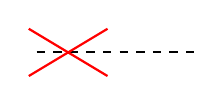
\begin{tikzpicture}
    \begin{feynman}
        \vertex (a);
        \vertex[right=2cm of a] (b);
        \diagram* {
            (a) -- [scalar] (b),
        };
    \end{feynman}
    \draw[red, thick] (0.9,0.3) -- (-0.1,-0.3);
    \draw[red, thick] (-0.1,0.3) -- (0.9,-0.3);
\end{tikzpicture}
\caption{重整化的图形表示：裸传播子 = 物理传播子 + 自能修正 + 抵消项。红色叉号表示抵消项顶点。}
\label{fig:renormalization}
\end{figure}

\begin{theorem}[重整化条件]
抵消项由 \textbf{重整化条件} 确定。常用的方案有：

\textbf{(1) 在壳重整化}（on-shell scheme）：要求传播子在物理质量处有极点且留数为 1：
\begin{align}
    \Sigma(p^2 = -m_R^2) &= 0, \\
    \left.\frac{d\Sigma}{dp^2}\right|_{p^2=-m_R^2} &= 0.
\end{align}

\textbf{(2) $\overline{\rm MS}$ 方案}（modified minimal subtraction）：只减去 $1/\epsilon$ 极点及相关的常数 $\ln(4\pi) - \gamma_E$（其中 $\gamma_E$ 是 Euler 常数）。这是粒子物理中最常用的方案，因为它保持了过程的简单性。
\end{theorem}

%------ 重整化群 ------

\subsection{重整化群与 $\beta$ 函数}

重整化引入了一个任意的质量尺度 $\mu$（维数正规化尺度或重整化点）。物理可观测量不依赖于 $\mu$ 的选择，这一要求导出了 \textbf{重整化群方程}（RGE）。

\begin{theorem}[Callan--Symanzik 方程]
$n$ 点关联函数 $G^{(n)}$ 满足 Callan--Symanzik 方程：
\begin{equation}
    \left[\mu\frac{\partial}{\partial\mu} + \beta(g)\frac{\partial}{\partial g} + n\gamma(g)\right]G^{(n)}(p_i; g, \mu) = 0,
\end{equation}
其中：
\begin{itemize}
    \item $\beta(g) = \mu\dfrac{dg}{d\mu}$ 是 \textbf{$\beta$ 函数}，描述耦合常数随尺度的变化
    \item $\gamma(g) = \dfrac{1}{2}\mu\dfrac{d\ln Z_\phi}{d\mu}$ 是 \textbf{反常量纲}（anomalous dimension），描述场的标度行为的修正
\end{itemize}
\end{theorem}

\begin{proof}[ $\beta$ 函数的推导（$\phi^4$ 理论，单圈）]
在 $\phi^4$ 理论中，单圈 $\beta$ 函数可以通过以下步骤推导：

\textbf{第一步}：在维数正规化下，裸耦合与重整化耦合的关系为：
\begin{equation}
    \lambda_0 = \mu^\epsilon\left(\lambda_R + \frac{3\lambda_R^2}{16\pi^2}\frac{1}{\epsilon} + \cdots\right).
\end{equation}
因子 $3$ 来自于 $\phi^4$ 理论中四点函数的三个通道（$s, t, u$）。

\textbf{第二步}：裸耦合不依赖于 $\mu$，因此 $\mu\dfrac{d\lambda_0}{d\mu} = 0$。

\textbf{第三步}：对上式求 $\mu$ 的导数：
\begin{equation}
    0 = \epsilon\mu^\epsilon\left(\lambda_R + \cdots\right) + \mu^\epsilon\left(\frac{d\lambda_R}{d\mu} + \frac{6\lambda_R}{16\pi^2}\frac{1}{\epsilon}\frac{d\lambda_R}{d\mu} + \cdots\right).
\end{equation}

\textbf{第四步}：令 $\epsilon \to 0$，解出 $\beta$ 函数：
\begin{equation}
    \beta(\lambda) = \mu\frac{d\lambda}{d\mu} = \frac{3\lambda^2}{16\pi^2} + \mathcal{O}(\lambda^3).
\end{equation}

由于 $\beta(\lambda) > 0$，$\phi^4$ 理论的耦合常数随能量增大而增大——在高能下理论变得强耦合。
\end{proof}

\begin{property}[跑动耦合常数]
$\beta$ 函数决定了耦合常数的"跑动"（running）。将 RGE 积分：
\begin{equation}
    \frac{1}{\lambda(\mu)} = \frac{1}{\lambda(\mu_0)} - \frac{3}{16\pi^2}\ln\frac{\mu}{\mu_0}.
\end{equation}
这表明：
\begin{itemize}
    \item $\beta > 0$（如 $\phi^4$ 理论）：$\lambda(\mu)$ 随 $\mu$ 增大而增大，高能下强耦合
    \item $\beta < 0$（如 QCD）：$\lambda(\mu)$ 随 $\mu$ 增大而减小，高能下弱耦合（渐近自由）
    \item $\beta = 0$（如 QED 的 $\beta$ 函数为正但很小）：耦合变化缓慢
\end{itemize}
\end{property}

\begin{figure}[htbp]
\centering
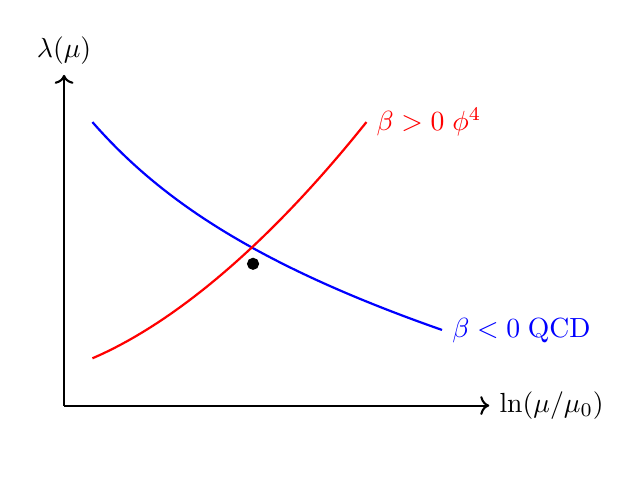
\begin{tikzpicture}[scale=1.2]
    % Axes
    \draw[->] (0,0) -- (4.5,0) node[right] {$\ln(\mu/\mu_0)$};
    \draw[->] (0,0) -- (0,3.5) node[above] {$\lambda(\mu)$};
    % QCD-like (asymptotically free)
    \draw[thick, blue] (0.3,3) .. controls (1,2.2) and (2,1.5) .. (4,0.8);
    \node[blue, right] at (4,0.8) {$\beta < 0$（QCD）};
    % phi^4 theory
    \draw[thick, red] (0.3,0.5) .. controls (1,0.8) and (2,1.5) .. (3.2,3);
    \node[red, right] at (3.2,3) {$\beta > 0$（$\phi^4$）};
    % Fixed point
    \filldraw (2,1.5) circle (1.5pt) node[above right] {不动点};
    % Labels
    \node at (0.5,-0.5) {低能};
    \node at (3.5,-0.5) {高能};
\end{tikzpicture}
\caption{跑动耦合常数的示意图。$\beta < 0$（如 QCD）时耦合在高能下减小（渐近自由）；$\beta > 0$（如 $\phi^4$ 理论）时耦合在高能下增大。}
\label{fig:running_coupling}
\end{figure}

\begin{remark}[Wilson 重整化群]
Kenneth Wilson 提出了重整化群的物理图像：逐步"积掉"高能自由度，观察低能有效理论如何变化。

具体来说，将场分解为低能模（$|k| < \Lambda/b$）和高能模（$\Lambda/b < |k| < \Lambda$），对高能模做路径积分：
\begin{equation}
    e^{-S_{\rm eff}[\phi_<]} = \int\mathcal{D}\phi_>\, e^{-S[\phi_<+\phi_>]}.
\end{equation}
这导致了有效作用量中参数的"流动"，正是 $\beta$ 函数所描述的。

Wilson 的观点深刻地揭示了重整化的物理本质：它不是简单地"消除无穷大"，而是描述了物理规律在不同能量尺度上的变化。
\end{remark}

%------ 渐近自由 ------

\begin{note}[渐近自由]
\textbf{渐近自由}（asymptotic freedom）：当 $\beta(g) < 0$ 时，耦合常数在高能下变小。

1973 年，Gross、Wilczek 和 Politzer 独立发现非阿贝尔规范理论（如 QCD）具有渐近自由的性质 \cite{Gross1973,Politzer1973}。QCD 的单圈 $\beta$ 函数为：
\begin{equation}
    \beta(g_s) = -\frac{g_s^3}{16\pi^2}\left(11 - \frac{2}{3}N_f\right),
\end{equation}
其中 $g_s$ 是强耦合常数，$N_f$ 是夸克味数。当 $N_f \leq 16$ 时 $\beta < 0$，理论渐近自由。

渐近自由的物理后果：
\begin{itemize}
    \item \textbf{高能}：夸克和胶子行为接近自由粒子（微扰 QCD 可靠）
    \item \textbf{低能}：耦合变强，导致 \textbf{色禁闭}（quark confinement）
\end{itemize}
这一发现获得了 2004 年 Nobel 物理学奖。
\end{note}

%------ 可重整性与有效场论 ------

\subsection{可重整性与有效场论}

\begin{definition}[可重整与不可重整]
一个理论的 \textbf{可重整性}（renormalizability）指的是：是否只需要有限个抵消项就能消除所有阶的发散。
\begin{itemize}
    \item \textbf{可重整理论}（renormalizable）：如 $\phi^4$ 理论、QED、QCD——只有有限种发散图，需要有限个抵消项
    \item \textbf{不可重整理论}（non-renormalizable）：如广义相对论、费米弱相互作用——每一阶都需要新的抵消项
    \item \textbf{渐近安全理论}（asymptotically safe）：尽管不可重整，但在 UV 有非高斯不动点，使得理论在高能下仍然有意义
\end{itemize}
\end{definition}

\begin{remark}[有效场论的观点]
从 Wilson 的角度来看，"不可重整"并不意味着理论无用，而只是表明它是一个 \textbf{有效场论}（effective field theory, EFT）——在某个能量尺度 $\Lambda$ 以下有效。高能效应被"编码"在低能耦合常数中。

例如，费米弱相互作用理论（四费米子耦合）的截断尺度 $\Lambda \sim M_W \sim 100$ GeV（$W$ 玻色子质量），在这个尺度以下它是优秀的有效理论。

这一观点深刻地改变了我们对理论物理的理解：我们不需要一个"万有理论"，只需要在每个能量尺度上使用正确的有效理论。
\end{remark}

%------ 量子反常 ------

\subsection{量子反常}

\begin{definition}[量子反常]
\textbf{量子反常}（quantum anomaly）：经典对称性在量子水平上被破坏的现象。反常的出现是因为路径积分测度 $\mathcal{D}\phi$ 不保持经典对称性。
\end{definition}

\begin{example}[三角形反常]
\textbf{三角形反常}（triangle anomaly / ABJ anomaly）：考虑一个费米子三角形图（三个轴矢量流的关联函数），在经典水平上手征对称性 $j_5^\mu = \bar{\psi}\gamma^\mu\gamma_5\psi$ 是守恒的，但量子修正导致：
\begin{equation}
    \partial_\mu j_5^\mu = \frac{e^2}{16\pi^2}F_{\mu\nu}\tilde{F}^{\mu\nu},
\end{equation}
其中 $\tilde{F}^{\mu\nu} = \frac{1}{2}\epsilon^{\mu\nu\rho\sigma}F_{\rho\sigma}$ 是对偶场强张量。

这一反常有重要的物理后果：它解释了 $\pi^0 \to 2\gamma$ 衰变，也保证了 QCD 中 $U(1)_A$ 对称性的破缺。
\end{example}

\begin{remark}[共形反常与 AdS/CFT]
\textbf{共形反常}（conformal anomaly / trace anomaly）：在偶数维 CFT 中，应力张量的迹不为零：
\begin{equation}
    \langle T^\mu{}_\mu \rangle = a \cdot E_d + c \cdot W^2 + \cdots
\end{equation}
其中 $E_d$ 是 Euler 密度，$W^2$ 是 Weyl 张量的平方，$a$ 和 $c$ 是中心荷。

在 AdS/CFT 中，共形反常可以通过全息重整化（holographic renormalization）从引力侧计算 \cite{Henningson1998}。具体来说，AdS 空间的体积发散对应于 CFT 的紫外发散，通过在边界附近引入抵消项（counterterm action），可以得到有限的 Brown-York 应力张量 \cite{Balasubramanian1999}。

这一联系是 AdS/CFT 对偶最精妙的应用之一：引力中的几何操作（截断 + 抵消）精确地对应于场论中的重整化。
\end{remark}

\section{配分函数与 AdS/CFT}

\begin{theorem}[AdS/CFT 对偶中的配分函数]
在 AdS/CFT 对偶中，CFT 的配分函数与引力理论的配分函数等价：
\begin{equation}
    Z_{\rm CFT}[J] = Z_{\rm gravity}[\phi \to J \text{ at boundary}].
\end{equation}

这个等价性意味着：
\begin{itemize}
    \item CFT 的关联函数可以通过计算引力理论的经典解得到
    \item CFT 的有效作用量对应于引力理论的 on-shell 作用量
    \item CFT 的重整化群流对应于引力理论的径向演化
\end{itemize}
\end{theorem}

\begin{note}[配分函数的统一视角]
配分函数是贯穿整个理论物理的核心概念：
\begin{itemize}
    \item \textbf{统计力学}：配分函数 $Z = \Tr e^{-\beta H}$ 包含了所有热力学信息
    \item \textbf{量子场论}：配分函数 $Z[J]$ 是所有关联函数的生成泛函
    \item \textbf{AdS/CFT}：$Z_{\rm CFT} = Z_{\rm gravity}$ 将引力理论与量子场论联系起来
\end{itemize}
这种统一性表明，配分函数是理解自然界最深刻的工具之一。
\end{note}

\section{小结}

在本节中，我们介绍了量子场论中配分函数的核心地位：
\begin{itemize}
    \item 量子场论的基本对象是场算符，作用量决定了系统的动力学
    \item 路径积分量子化通过对所有场构型求和来表述量子理论
    \item 配分函数是所有关联函数的生成泛函
    \item 连通关联函数和 1PI 关联函数可以通过生成泛函的泛函微分得到
    \item 有效作用量包含了所有量子修正的贡献
    \item 费曼图是计算关联函数的图形方法
    \item 重整化是处理发散的系统方法
\end{itemize}

%=============================================================================


\chapter{应力张量 (Stress-Energy Tensor)}

%=============================================================================

应力张量（stress-energy tensor）$T_{\mu\nu}(x)$ 是理论物理中最基本的算符之一。它描述了能量和动量在时空中的分布，是连接引力与量子场论的桥梁。在广义相对论中，应力张量是爱因斯坦场方程的源项；在量子场论中，它是守恒流的推广；在共形场论中，它的迹与共形异常密切相关；在 AdS/CFT 对偶中，它对应于体空间中的度规扰动\cite{Balasubramanian1999}。本节将系统地介绍应力张量的定义、性质和物理意义。

\section{应力张量的物理图像}

在介绍数学定义之前，我们先建立应力张量的物理直觉。

\subsection{从连续力学到场论}

在连续介质力学中，应力张量描述了介质内部的应力状态。考虑一个流体元，我们需要知道：
\begin{itemize}
    \item 这个流体元包含多少能量？→ $T_{00}$：能量密度
    \item 能量在如何流动？→ $T_{0i}$：能量流密度（或动量密度）
    \item 流体内部的应力如何？→ $T_{ij}$：动量流密度，即应力
\end{itemize}

\begin{figure}[htbp]
\centering
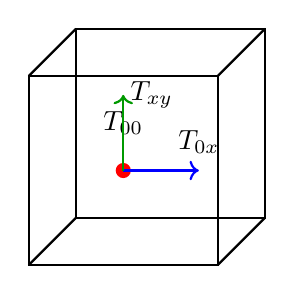
\begin{tikzpicture}[scale=1.2]
    % 绘制立方体
    \draw[thick] (0,0) -- (2,0) -- (2,2) -- (0,2) -- cycle;
    \draw[thick] (0.5,0.5) -- (2.5,0.5) -- (2.5,2.5) -- (0.5,2.5) -- cycle;
    \draw[thick] (0,0) -- (0.5,0.5);
    \draw[thick] (2,0) -- (2.5,0.5);
    \draw[thick] (0,2) -- (0.5,2.5);
    \draw[thick] (2,2) -- (2.5,2.5);
    
    % 标注 T_00
    \fill[red] (1,1) circle (0.08);
    \node at (1,1.5) {$T_{00}$};
    \node at (1,1.2) {\footnotesize 能量密度};
    
    % 标注 T_0i
    \draw[->, blue, thick] (1,1) -- (1.8,1);
    \node at (1.8,1.3) {$T_{0x}$};
    \node at (1.8,0.8) {\footnotesize 能量流};
    
    % 标注 T_ij
    \draw[->, green!60!black, thick] (1,1) -- (1,1.8);
    \node at (1.3,1.8) {$T_{xy}$};
    \node at (1.3,1.5) {\footnotesize 剪应力};
\end{tikzpicture}
\caption{应力张量分量的物理意义。$T_{00}$ 是能量密度，$T_{0i}$ 描述能量流动，$T_{ij}$ 描述应力状态。}
\label{fig:stress_tensor_components}
\end{figure}

\subsection{从力学到场论的推广}

在场论中，应力张量是能量-动量四矢量 $P^\mu$ 的流密度。考虑一个超曲面 $\Sigma$，通过它的能量-动量流为：
\begin{equation}
    P^\mu = \int_\Sigma d^3x \, T^{0\mu}.
\end{equation}
这表明应力张量是"能量-动量的密度和流"的统一描述。

\subsection{应力张量守恒的物理图像}

应力张量的守恒可以用直观的物理图像理解。考虑一个区域 $\Omega$，其内部的能量-动量只能通过边界流入或流出。

\begin{figure}[htbp]
\centering
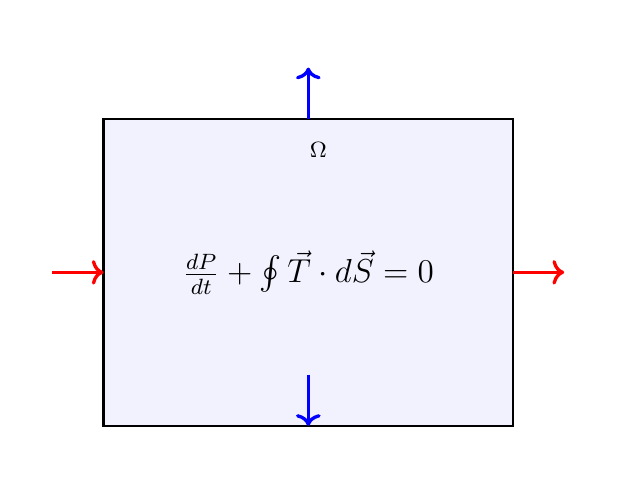
\begin{tikzpicture}[scale=1.3]
    % 绘制区域
    \draw[thick, fill=blue!5] (0,0) rectangle (4,3);
    \node at (2,2.7) {\footnotesize 区域 $\Omega$};
    
    % 入射动量流
    \draw[->, red, very thick] (-0.5,1.5) -- (0,1.5);
    \node at (-0.5,1.9) {\footnotesize 入射动量流};
    
    % 出射动量流
    \draw[->, red, very thick] (4,1.5) -- (4.5,1.5);
    \node at (4.5,1.9) {\footnotesize 出射动量流};
    
    % 上方能量流出
    \draw[->, blue, very thick] (2,3) -- (2,3.5);
    \node at (2,3.8) {\footnotesize 能量流出};
    
    % 下方能量流入
    \draw[->, blue, very thick] (2,0.5) -- (2,0);
    \node at (2,-0.3) {\footnotesize 能量流入};
    
    % 标注守恒
    \node at (2,1.5) {\large $\frac{dP}{dt} + \oint \vec{T} \cdot d\vec{S} = 0$};
\end{tikzpicture}
\caption{应力张量守恒的物理图像。区域内的能量-动量变化率等于通过边界流入的动量流。}
\label{fig:stress_conservation}
\end{figure}

\begin{note}[守恒律的直观理解]
应力张量的守恒方程 $\partial^\mu T_{\mu\nu} = 0$ 的物理含义是：能量和动量不能凭空产生或消失，只能从一个地方流到另一个地方。这类似于流体力学中的连续性方程：流体的密度变化率等于流入的流量。
\end{note}

\section{经典应力张量}

\subsection{应力张量的定义}

在定义应力张量之前，我们先说明其物理动机。在广义相对论中，爱因斯坦场方程将时空几何与能量-动量分布联系起来：
\begin{equation}
    R_{\mu\nu} - \frac{1}{2} g_{\mu\nu} R + \Lambda g_{\mu\nu} = 8\pi G_N T_{\mu\nu}.
\end{equation}
因此，应力张量自然地出现在引力理论中。在量子场论中，即使没有引力，我们仍然可以通过对度规变分来定义应力张量，这是因为应力张量是庞加莱对称性的守恒流。

\begin{definition}[应力张量]
对于场 $\phi$ 的理论，应力张量定义为作用量对度规的变分：
\begin{equation}
    T_{\mu\nu}(x) = -\frac{2}{\sqrt{-g}} \frac{\delta S}{\delta g^{\mu\nu}(x)}.
\end{equation}
这个定义在弯曲时空和闵可夫斯基时空中都适用。在闵可夫斯基时空中，我们取 $g_{\mu\nu} = \eta_{\mu\nu}$。
\end{definition}

\begin{note}[为什么是对度规变分？]
应力张量定义为作用量对度规的变分，这不是偶然的。物理上，度规决定了时空的几何，而应力张量描述了能量-动量的分布。在广义相对论中，爱因斯坦方程将两者联系起来。因此，应力张量自然地出现在引力理论中。在量子场论中，即使没有引力，我们仍然可以通过对度规变分来定义应力张量，这是因为应力张量是庞加莱对称性的守恒流。
\end{note}

\subsection{标量场的应力张量}

\begin{example}[标量场的应力张量]
考虑标量场 $\phi$，作用量为：
\begin{equation}
    S = \int d^d x \sqrt{-g} \left[\frac{1}{2} g^{\mu\nu} \partial_\mu \phi \partial_\nu \phi - V(\phi)\right].
\end{equation}

对度规 $g^{\mu\nu}$ 求变分：
\begin{equation}
    \delta S = \int d^d x \sqrt{-g} \left[\frac{1}{2} \delta g^{\mu\nu} \partial_\mu \phi \partial_\nu \phi + \left(\frac{1}{2} g^{\mu\nu} \partial_\mu \phi \partial_\nu \phi - V\right) \frac{\delta \sqrt{-g}}{\sqrt{-g}}\right].
\end{equation}

利用 $\delta \sqrt{-g} = -\frac{1}{2} \sqrt{-g} g_{\mu\nu} \delta g^{\mu\nu}$，得到：
\begin{equation}
    \delta S = \int d^d x \sqrt{-g} \left[\frac{1}{2} \partial_\mu \phi \partial_\nu \phi - \frac{1}{2} g_{\mu\nu} \left(\frac{1}{2} g^{\rho\sigma} \partial_\rho \phi \partial_\sigma \phi - V\right)\right] \delta g^{\mu\nu}.
\end{equation}

因此应力张量为：
\begin{equation}
    T_{\mu\nu} = \partial_\mu \phi \partial_\nu \phi - g_{\mu\nu} \left[\frac{1}{2} g^{\rho\sigma} \partial_\rho \phi \partial_\sigma \phi - V(\phi)\right].
\end{equation}

在闵可夫斯基时空中，$g_{\mu\nu} = \eta_{\mu\nu}$，$\mathcal{L} = \frac{1}{2}(\partial_\mu \phi)^2 - V(\phi)$，所以：
\begin{equation}
    T_{\mu\nu} = \partial_\mu \phi \partial_\nu \phi - \eta_{\mu\nu} \mathcal{L}.
\end{equation}
\end{example}

\begin{note}[标量场应力张量的物理意义]
标量场的应力张量 $T_{\mu\nu} = \partial_\mu \phi \partial_\nu \phi - \eta_{\mu\nu} \mathcal{L}$ 有清晰的物理解释：
\begin{itemize}
    \item $T_{00} = \frac{1}{2}\dot{\phi}^2 + \frac{1}{2}(\nabla\phi)^2 + V(\phi)$：能量密度，包含动能、梯度能和势能
    \item $T_{0i} = \dot{\phi} \partial_i \phi$：能量流密度，描述能量如何在空间中流动
    \item $T_{ij} = \partial_i \phi \partial_j \phi - \delta_{ij} \mathcal{L}$：应力，描述场的"压力"
\end{itemize}
\end{note}

\subsection{电磁场的应力张量}

\begin{example}[电磁场的应力张量]
电磁场的作用量为：
\begin{equation}
    S = -\frac{1}{4} \int d^d x \sqrt{-g} g^{\mu\rho} g^{\nu\sigma} F_{\mu\nu} F_{\rho\sigma}.
\end{equation}

对度规求变分，注意 $F_{\mu\nu}$ 不依赖于度规：
\begin{equation}
    \delta S = -\frac{1}{4} \int d^d x \sqrt{-g} \left[2 \delta g^{\mu\rho} g^{\nu\sigma} F_{\mu\nu} F_{\rho\sigma} - g^{\mu\rho} g^{\nu\sigma} F_{\mu\nu} F_{\rho\sigma} g_{\alpha\beta} \delta g^{\alpha\beta}\right].
\end{equation}

整理得：
\begin{equation}
    \delta S = -\frac{1}{2} \int d^d x \sqrt{-g} \left[F_{\mu\rho} F_\nu^{~\rho} - \frac{1}{4} g_{\mu\nu} F_{\rho\sigma} F^{\rho\sigma}\right] \delta g^{\mu\nu}.
\end{equation}

因此电磁场的应力张量为：
\begin{equation}
    T_{\mu\nu} = F_{\mu\rho} F_\nu^{~\rho} - \frac{1}{4} g_{\mu\nu} F_{\rho\sigma} F^{\rho\sigma}.
\end{equation}
\end{example}

\begin{note}[电磁场应力张量的性质]
电磁场的应力张量具有几个重要性质：
\begin{itemize}
    \item \textbf{无迹性}：$T_\mu^{~\mu} = 0$，这反映了电磁场的共形不变性
    \item \textbf{对称性}：$T_{\mu\nu} = T_{\nu\mu}$，这是由电磁场张量的对称性保证的
    \item \textbf{正能量密度}：$T_{00} = \frac{1}{2}(E^2 + B^2) \geq 0$，这保证了能量的正定性
\end{itemize}
\end{note}

\section{守恒律与对称性}

\subsection{从 Noether 定理到能量-动量守恒}

Noether 定理告诉我们，每一个连续对称性都对应一个守恒律。时空平移对称性对应能量-动量守恒。下面我们从 Noether 定理出发，推导应力张量的守恒律。

\begin{theorem}[能量-动量守恒]
应力张量满足守恒方程：
\begin{equation}
    \partial^\mu T_{\mu\nu} = 0.
\end{equation}
这个方程表达了能量-动量守恒：能量和动量不能凭空产生或消失，只能从一个地方流到另一个地方。这是物理学中最基本的守恒律之一。
\end{theorem}

\begin{proof}[能量-动量守恒的推导]
考虑场论的作用量 $S[\phi, g]$，其中 $\phi$ 是场，$g$ 是度规。在无穷小坐标变换 $x^\mu \to x^\mu + \epsilon^\mu$ 下，场的变化为：
\begin{equation}
    \delta \phi = -\epsilon^\mu \partial_\mu \phi, \qquad \delta g_{\mu\nu} = -\epsilon^\rho \partial_\rho g_{\mu\nu} - g_{\mu\rho} \partial_\nu \epsilon^\rho - g_{\nu\rho} \partial_\mu \epsilon^\rho.
\end{equation}

作用量的变化为零（对称性）：
\begin{equation}
    \delta S = \int d^d x \left[\frac{\delta S}{\delta \phi} \delta \phi + \frac{\delta S}{\delta g^{\mu\nu}} \delta g^{\mu\nu}\right] = 0.
\end{equation}

利用运动方程 $\frac{\delta S}{\delta \phi} = 0$，得到：
\begin{equation}
    \delta S = -\frac{1}{2} \int d^d x \sqrt{-g} T_{\mu\nu} \delta g^{\mu\nu} = 0.
\end{equation}

将 $\delta g^{\mu\nu}$ 的表达式代入，经过分部积分，得到：
\begin{equation}
    \int d^d x \sqrt{-g} \epsilon^\nu \nabla^\mu T_{\mu\nu} = 0.
\end{equation}

由于 $\epsilon^\nu$ 是任意的，我们得到守恒方程：
\begin{equation}
    \nabla^\mu T_{\mu\nu} = 0.
\end{equation}

在平直时空中，$\nabla^\mu \to \partial^\mu$，因此 $\partial^\mu T_{\mu\nu} = 0$。
\end{proof}

\begin{note}[守恒律的物理意义]
守恒方程的积分形式为：
\begin{equation}
    \frac{d}{dt} \int d^3x \, T_{00} = -\int d^3x \, \partial_i T_{0i}.
\end{equation}
左边是总能量的时间变化率，右边是通过边界流入的能量。这表明：能量可以从一个地方流到另一个地方，但总能量守恒。
\end{note}

\subsection{角动量守恒}

应力张量的对称性 $T_{\mu\nu} = T_{\nu\mu}$ 保证了角动量守恒。角动量密度定义为：
\begin{equation}
    M^{\mu\nu\rho} = x^\nu T^{\mu\rho} - x^\rho T^{\mu\nu}.
\end{equation}

\begin{theorem}[角动量守恒]
利用 $\partial^\mu T_{\mu\nu} = 0$ 和 $T_{\mu\nu} = T_{\nu\mu}$，可以验证：
\begin{equation}
    \partial_\mu M^{\mu\nu\rho} = 0,
\end{equation}
即角动量守恒。
\end{theorem}

\begin{proof}[角动量守恒的推导]
计算散度：
\begin{equation}
    \partial_\mu M^{\mu\nu\rho} = \partial_\mu (x^\nu T^{\mu\rho} - x^\rho T^{\mu\nu}).
\end{equation}

利用乘积法则：
\begin{equation}
    \partial_\mu (x^\nu T^{\mu\rho}) = (\partial_\mu x^\nu) T^{\mu\rho} + x^\nu (\partial_\mu T^{\mu\rho}) = \delta_\mu^\nu T^{\mu\rho} + x^\nu (\partial_\mu T^{\mu\rho}).
\end{equation}

由于 $\partial_\mu T^{\mu\rho} = 0$，第一项为 $T^{\nu\rho}$。类似地，第二项为 $T^{\rho\nu}$。因此：
\begin{equation}
    \partial_\mu M^{\mu\nu\rho} = T^{\nu\rho} - T^{\rho\nu} = 0,
\end{equation}
其中最后一步利用了应力张量的对称性 $T_{\mu\nu} = T_{\nu\mu}$。
\end{proof}

\begin{note}[对称性与守恒律的对应]
根据 Noether 定理，每一个连续对称性都对应一个守恒律：
\begin{itemize}
    \item 时间平移对称性 $\to$ 能量守恒（$T_{00}$ 的积分）
    \item 空间平移对称性 $\to$ 动量守恒（$T_{0i}$ 的积分）
    \item 旋转对称性 $\to$ 角动量守恒（$M^{\mu\nu\rho}$ 的积分）
\end{itemize}
应力张量统一描述了这些守恒律。
\end{note}

\section{应力张量的量子性质}

在量子场论中，应力张量被提升为算符 $\hat{T}_{\mu\nu}(x)$。

\subsection{量子应力张量的基本性质}

\begin{property}[量子应力张量的性质]
应力张量是厄米算符：$\hat{T}_{\mu\nu}^\dagger = \hat{T}_{\mu\nu}$。在类空间隔处，应力张量与其他算符对易：
\begin{equation}
    [\hat{T}_{\mu\nu}(x), \hat{T}_{\rho\sigma}(y)] = 0 \quad \text{for} \quad (x-y)^2 > 0.
\end{equation}
这是因果性（causality）的要求：类空间隔处的测量不能相互影响。
\end{property}

在真空中，应力张量的期望值为零：
\begin{equation}
    \langle 0 | \hat{T}_{\mu\nu}(x) | 0 \rangle = 0,
\end{equation}
这是因为在闵可夫斯基时空中，真空是庞加莱不变的。

\subsection{应力张量的 OPE}

应力张量的算符乘积展开（OPE）包含重要的物理信息。例如，应力张量与自身的 OPE 为：
\begin{equation}
    T_{\mu\nu}(x) T_{\rho\sigma}(0) \sim \frac{c/2}{x^{2d}} I_{\mu\nu,\rho\sigma} + \frac{A}{x^{d}} T_{\mu\nu}(0) + \cdots
\end{equation}
其中 $c$ 是中心荷（central charge），$A$ 是常数。

\begin{note}[中心荷的物理意义]
中心荷 $c$ 度量了理论的"自由度"，是 CFT 中最重要的参数之一。在 2 维 CFT 中，中心荷直接对应于理论的自由度数。例如，自由标量场的 $c = 1$，自由费米子的 $c = 1/2$。在 AdS/CFT 对偶中，中心荷与引力常数相关：$c \sim L^{d-1}/G_N$。
\end{note}

\section{应力张量与共形对称性}

在共形场论中，应力张量具有特殊的性质。

\subsection{共形代数的生成元}

应力张量是共形代数的生成元。具体来说，通过对应力张量在空间上积分，我们可以得到共形代数的所有生成元：
\begin{itemize}
    \item 平移生成元：$P_\mu = \int d^{d-1}x \, T_{0\mu}$
    \item 旋转生成元：$M_{\mu\nu} = \int d^{d-1}x \, (x_\mu T_{0\nu} - x_\nu T_{0\mu})$
    \item 标度变换生成元：$D = \int d^{d-1}x \, x^\mu T_{0\mu}$
    \item 特殊共形变换生成元：$K_\mu = \int d^{d-1}x \, (2x_\mu x^\nu T_{0\nu} - x^2 T_{0\mu})$
\end{itemize}

\begin{note}[应力张量作为"生成元密度"]
这解释了为什么应力张量在 CFT 中如此重要：它是共形代数的"生成元密度"。通过对应力张量在空间上积分，我们可以得到共形代数的所有生成元。这使得应力张量成为 CFT 中最核心的算符。
\end{note}

\subsection{共形异常}

在量子水平上，应力张量的迹不为零，这被称为共形异常（conformal anomaly）：
\begin{equation}
    \langle T_\mu^{~\mu} \rangle = \frac{(-1)^{d/2}}{2} A E_d + \sum_i B_i I_i.
\end{equation}
共形异常反映了量子涨落破坏了经典共形对称性：即使经典理论是共形不变的，量子效应也会导致应力张量的迹不为零。

\begin{theorem}[共形异常的推导]
考虑共形场论在弯曲背景上的有效作用量 $W[g]$。在 Weyl 变换 $g_{\mu\nu} \to e^{2\sigma} g_{\mu\nu}$ 下，有效作用量的变化为：
\begin{equation}
    \delta_\sigma W = \int d^d x \sqrt{g} \, \sigma(x) \langle T_\mu^{~\mu} \rangle.
\end{equation}

在经典水平上，如果理论是共形不变的，则 $\delta_\sigma W = 0$，从而 $\langle T_\mu^{~\mu} \rangle = 0$。但在量子水平上，正规化和重整化过程会破坏共形不变性，导致：
\begin{equation}
    \langle T_\mu^{~\mu} \rangle = \frac{(-1)^{d/2}}{2} A E_d + \sum_i B_i I_i,
\end{equation}
其中 $E_d$ 是 Euler 密度，$I_i$ 是 Weyl 张量的不变量。在 $d=4$ 时：
\begin{equation}
    E_4 = R_{\mu\nu\rho\sigma} R^{\mu\nu\rho\sigma} - 4 R_{\mu\nu} R^{\mu\nu} + R^2, \qquad I_1 = C_{\mu\nu\rho\sigma} C^{\mu\nu\rho\sigma}.
\end{equation}
\end{theorem}

\begin{remark}[共形异常的物理意义]
共形异常反映了量子效应如何破坏经典对称性。即使经典理论是共形不变的，量子涨落也会导致应力张量的迹不为零。这是量子场论中"反常"现象的一个重要例子。
\end{remark}

\begin{note}[$a$-异常系数与 $a$-定理]
$a$-异常系数 $A$ 是 CFT 的重要参数。在 4 维中，$a$-异常系数沿着重整化群流单调递减（$a$-定理）\cite{Komargodski2011}：
\begin{equation}
    a_{\rm UV} > a_{\rm IR}.
\end{equation}
例如，自由标量场的 $a = 1/360$，自由费米子的 $a = 11/720$。$a$-定理告诉我们，在重整化群流中，系统的"自由度"单调递减。
\end{note}

\section{Ward 恒等式}

应力张量的守恒律和共形对称性导致了一系列重要的 Ward 恒等式。

\subsection{平移 Ward 恒等式}

\begin{theorem}[平移 Ward 恒等式]
考虑无穷小坐标变换 $\tilde{x}^\mu = x^\mu + \epsilon^\mu(x)$，度规的变化为 $\tilde{g}_{\mu\nu} = g_{\mu\nu} - \nabla_\mu \epsilon_\nu - \nabla_\nu \epsilon_\mu$。物理不应改变，这导致守恒方程：
\begin{equation}
    \nabla_\mu \langle T^{\mu\nu}(x) \rangle_g = 0,
\end{equation}
以及关联函数的 Ward 恒等式：
\begin{equation}
    \sum_{i=1}^n \epsilon^\mu(x_i) \frac{\partial}{\partial x_i^\mu} \langle \mathcal{O}_1(x_1) \cdots \mathcal{O}_n(x_n) \rangle_g = -\int dx \sqrt{g} \, \epsilon_\nu(x) \langle \nabla_\mu T^{\mu\nu}(x) \mathcal{O}_1(x_1) \cdots \mathcal{O}_n(x_n) \rangle_g.
\end{equation}
\end{theorem}

\begin{proof}[平移 Ward 恒等式的推导]
考虑关联函数 $\langle \mathcal{O}_1(x_1) \cdots \mathcal{O}_n(x_n) \rangle_g$。在无穷小坐标变换 $x^\mu \to x^\mu + \epsilon^\mu(x)$ 下，关联函数的变化为：
\begin{equation}
    \delta \langle \mathcal{O}_1(x_1) \cdots \mathcal{O}_n(x_n) \rangle_g = -\sum_{i=1}^n \epsilon^\mu(x_i) \frac{\partial}{\partial x_i^\mu} \langle \mathcal{O}_1(x_1) \cdots \mathcal{O}_n(x_n) \rangle_g.
\end{equation}

另一方面，根据应力张量的定义，关联函数的变化也可以表示为：
\begin{equation}
    \delta \langle \mathcal{O}_1(x_1) \cdots \mathcal{O}_n(x_n) \rangle_g = \int dx \sqrt{g} \, \epsilon_\nu(x) \langle \nabla_\mu T^{\mu\nu}(x) \mathcal{O}_1(x_1) \cdots \mathcal{O}_n(x_n) \rangle_g.
\end{equation}

比较两个表达式，得到 Ward 恒等式。
\end{proof}

\subsection{Weyl Ward 恒等式}

\begin{theorem}[Weyl Ward 恒等式]
考虑无穷小 Weyl 变换 $\Omega = 1 + \omega$，对应度规变化 $\delta g_{\mu\nu} = 2\omega g_{\mu\nu}$。对于共形维数为 $\Delta_i$ 的算符，Weyl Ward 恒等式为：
\begin{equation}
    \sum_{i=1}^n \Delta_i \, \omega(x_i) \langle \mathcal{O}_1(x_1) \cdots \mathcal{O}_n(x_n) \rangle_g = -\int dx \sqrt{g} \, \omega(x) g_{\mu\nu} \langle T^{\mu\nu}(x) \mathcal{O}_1(x_1) \cdots \mathcal{O}_n(x_n) \rangle_g.
\end{equation}
这个恒等式表明，应力张量的迹 $T_\mu^{~\mu}$ 描述了关联函数在 Weyl 变换下的响应。
\end{theorem}

\begin{proof}[Weyl Ward 恒等式的推导]
在 Weyl 变换 $g_{\mu\nu} \to e^{2\omega} g_{\mu\nu} \approx (1+2\omega) g_{\mu\nu}$ 下，关联函数的变化为：
\begin{equation}
    \delta_\omega \langle \mathcal{O}_1(x_1) \cdots \mathcal{O}_n(x_n) \rangle_g = -\sum_{i=1}^n \Delta_i \, \omega(x_i) \langle \mathcal{O}_1(x_1) \cdots \mathcal{O}_n(x_n) \rangle_g.
\end{equation}

另一方面，根据应力张量的定义：
\begin{equation}
    \delta_\omega \langle \mathcal{O}_1(x_1) \cdots \mathcal{O}_n(x_n) \rangle_g = \int dx \sqrt{g} \, \omega(x) g_{\mu\nu} \langle T^{\mu\nu}(x) \mathcal{O}_1(x_1) \cdots \mathcal{O}_n(x_n) \rangle_g.
\end{equation}

比较两个表达式，得到 Weyl Ward 恒等式。
\end{proof}

\subsection{共形 Ward 恒等式}

\begin{theorem}[共形 Ward 恒等式]
对于共形变换，应力张量的守恒导致更精细的约束。考虑以原点为中心、半径为 $r$ 的球面 $\partial B$，共形 Ward 恒等式为：
\begin{equation}
    \int_{\partial B} dS_\mu \epsilon_\nu \langle T^{\mu\nu}(x) \mathcal{O}_1(x_1) \cdots \mathcal{O}_n(x_n) \rangle = -\sum_{x_i \in B} \left[\epsilon^\mu(x_i) \frac{\partial}{\partial x_i^\mu} + \frac{\Delta_i}{d} \nabla_\alpha \epsilon^\alpha(x_i)\right] \langle \mathcal{O}_1(x_1) \cdots \mathcal{O}_n(x_n) \rangle.
\end{equation}
这个恒等式将应力张量的通量与算符在共形变换下的响应联系起来。
\end{theorem}

\begin{remark}[共形 Ward 恒等式的物理意义]
共形 Ward 恒等式是共形场论中最重要的约束之一。它表明，应力张量的通量完全由算符在共形变换下的响应决定。这使得我们可以通过研究应力张量的关联函数来确定共形场论的性质。
\end{remark}

\section{应力张量的关联函数}

应力张量的关联函数包含 CFT 的重要信息。

\subsection{两点函数}

\begin{theorem}[应力张量的两点函数]
应力张量的两点函数由共形对称性完全确定：
\begin{equation}
    \langle T_{\mu\nu}(x) T_{\rho\sigma}(y) \rangle = C_T \frac{I_{\mu\nu,\rho\sigma}(x-y)}{|x-y|^{2d}},
\end{equation}
其中 $C_T$ 是应力张量的中心荷，$I_{\mu\nu,\rho\sigma}$ 是共形不变张量：
\begin{equation}
    I_{\mu\nu,\rho\sigma}(x) = \frac{1}{2} \left[I_{\mu\rho}(x) I_{\nu\sigma}(x) + I_{\mu\sigma}(x) I_{\nu\rho}(x)\right] - \frac{1}{d} \delta_{\mu\nu} \delta_{\rho\sigma},
\end{equation}
其中 $I_{\mu\nu}(x) = \delta_{\mu\nu} - 2x_\mu x_\nu / x^2$。
\end{theorem}

\begin{proof}[两点函数的推导]
应力张量的两点函数由共形对称性确定。在共形变换下，应力张量的变换规律为：
\begin{equation}
    T_{\mu\nu}(x) \to \left|\frac{\partial x'}{\partial x}\right|^{2\Delta/d} \frac{\partial x^\rho}{\partial x'^\mu} \frac{\partial x^\sigma}{\partial x'^\nu} T_{\rho\sigma}(x'),
\end{equation}
其中 $\Delta = d$ 是应力张量的共形维数。

两点函数必须满足共形不变性：
\begin{equation}
    \langle T_{\mu\nu}(x) T_{\rho\sigma}(y) \rangle = \left|\frac{\partial x'}{\partial x}\right|^{2\Delta/d} \left|\frac{\partial y'}{\partial y}\right|^{2\Delta/d} \frac{\partial x^\alpha}{\partial x'^\mu} \frac{\partial x^\beta}{\partial x'^\nu} \frac{\partial y^\gamma}{\partial y'^\rho} \frac{\partial y^\delta}{\partial y'^\sigma} \langle T_{\alpha\beta}(x') T_{\gamma\delta}(y') \rangle.
\end{equation}

唯一满足这个约束的张量结构是 $I_{\mu\nu,\rho\sigma}(x-y) / |x-y|^{2d}$，因此两点函数的形式完全确定。
\end{proof}

\begin{note}[中心荷 $C_T$ 的物理意义]
中心荷 $C_T$ 度量了 CFT 的"自由度"，是 CFT 中最重要的参数之一。在 AdS/CFT 对偶中，中心荷与引力常数相关：
\begin{equation}
    C_T = \frac{d L^{d-1}}{16\pi G_N} \frac{\Gamma(d+1)}{\pi^{d/2} \Gamma(d/2)}.
\end{equation}
对于 $\mathcal{N}=4$ 超对称杨-米尔斯理论，$C_T = N_c^2 / 2$，与大 $N_c$ 极限下的结果一致。
\end{note}

\subsection{应力张量与标量算符的两点函数}

应力张量与标量算符的两点函数为零：
\begin{equation}
    \langle T_{\mu\nu}(x) \mathcal{O}(y) \rangle = 0,
\end{equation}
这是由共形对称性和守恒律共同保证的。

\begin{remark}[两点函数为零的原因]
应力张量与标量算符的两点函数为零，这是因为应力张量是无迹守恒张量，而标量算符是标量。在共形变换下，它们的变换规律不同，因此两点函数必须为零。这也可以从 Ward 恒等式直接推导出来。
\end{remark}

\subsection{三点函数}

\begin{theorem}[应力张量的三点函数]
应力张量与两个标量算符的三点函数由共形对称性确定：
\begin{equation}
    \langle \mathcal{O}(x_1) \mathcal{O}(x_2) T^{\mu\nu}(x_3) \rangle = C_{\mathcal{O}\mathcal{O}T} \frac{H^{\mu\nu}(x_1, x_2, x_3)}{|x_{12}|^{2\Delta - d + 2} |x_{13}|^{d-2} |x_{23}|^{d-2}},
\end{equation}
其中 $\Delta$ 是标量算符的共形维数，$C_{\mathcal{O}\mathcal{O}T}$ 是三点函数系数，$H^{\mu\nu}$ 定义为：
\begin{equation}
    H^{\mu\nu} = V^\mu V^\nu - \frac{1}{d} V_\alpha V^\alpha \delta^{\mu\nu}, \qquad V^\mu = \frac{x_{13}^\mu}{x_{13}^2} - \frac{x_{23}^\mu}{x_{23}^2}.
\end{equation}

利用 Ward 恒等式可以确定三点函数系数与标量算符维数的关系：
\begin{equation}
    C_{\mathcal{O}\mathcal{O}T} = -\frac{d\Delta}{d-1} \frac{1}{S_d},
\end{equation}
其中 $S_d = 2\pi^{d/2} / \Gamma(d/2)$ 是 $(d-1)$ 维单位球面的面积。
\end{theorem}

\begin{proof}[三点函数系数的推导]
利用 Ward 恒等式，我们可以确定三点函数系数 $C_{\mathcal{O}\mathcal{O}T}$。考虑应力张量与两个标量算符的三点函数，对 $x_3$ 求散度：
\begin{equation}
    \partial_\mu^{x_3} \langle \mathcal{O}(x_1) \mathcal{O}(x_2) T^{\mu\nu}(x_3) \rangle = -\sum_{i=1}^2 \delta^d(x_{3i}) \partial^\nu_{x_i} \langle \mathcal{O}(x_1) \mathcal{O}(x_2) \rangle.
\end{equation}

将三点函数的表达式代入左边，计算散度。右边是两点函数的导数，包含 $\delta$ 函数。比较两边，可以确定 $C_{\mathcal{O}\mathcal{O}T}$ 与 $\Delta$ 的关系：
\begin{equation}
    C_{\mathcal{O}\mathcal{O}T} = -\frac{d\Delta}{d-1} \frac{1}{S_d}.
\end{equation}
\end{proof}

\begin{note}[OPE 结构]
应力张量与标量算符的 OPE 为：
\begin{equation}
    T_{\mu\nu}(x) \mathcal{O}(0) \sim C_{\mathcal{O}\mathcal{O}T} \frac{H_{\mu\nu}(x)}{|x|^{2\Delta - d + 2}} \mathcal{O}(0) + \cdots
\end{equation}
这个 OPE 反映了应力张量如何"探测"标量算符的性质。物理上，应力张量的插入可以看作是对时空几何的微扰，它会影响其他算符的行为。
\end{note}

\section{应力张量与 AdS/CFT}

在 AdS/CFT 对偶中，应力张量扮演着核心角色。它是连接边界 CFT 与体空间引力理论的关键桥梁\cite{Balasubramanian1999}。

\subsection{度规扰动与应力张量的对应}

在 AdS/CFT 的字典中，边界 CFT 的应力张量算符 $T_{\mu\nu}$ 对应于体空间 AdS 中的度规扰动 $h_{\mu\nu}$。具体来说，考虑 AdS 度规的渐近展开：
\begin{equation}
    ds^2 = \frac{L^2}{z^2} \left(dz^2 + g_{\mu\nu}(x, z) dx^\mu dx^\nu\right),
\end{equation}
其中 $g_{\mu\nu}(x, z)$ 在边界 $z \to 0$ 附近的展开为\cite{deHaro2000}：
\begin{equation}
    g_{\mu\nu}(x, z) = g_{\mu\nu}^{(0)}(x) + z^2 g_{\mu\nu}^{(2)}(x) + \cdots + z^d g_{\mu\nu}^{(d)}(x) + h_{\mu\nu}(x) z^d \log z + \cdots
\end{equation}

\begin{figure}[htbp]
\centering
\begin{tikzpicture}[scale=1.4]
    % AdS 边界
    \draw[thick] (-3,0) -- (3,0);
    \node at (3.3,0) {\footnotesize AdS 边界};
    
    % AdS 体空间
    \draw[thick, dashed] (-3,0) .. controls (-2,-2) and (2,-2) .. (3,0);
    \node at (0,-2.3) {\footnotesize AdS 体空间};
    
    % 度规扰动
    \draw[->, red, very thick] (0,0) -- (0,-1.5);
    \node at (0.5,-0.8) {\footnotesize $h_{\mu\nu}$};
    
    % 边界度规
    \draw[->, blue, very thick] (-2,0) -- (-1,0);
    \node at (-1.5,0.3) {\footnotesize $g_{\mu\nu}^{(0)}$};
    
    % 应力张量
    \draw[->, green!60!black, very thick] (2,0) -- (1,0);
    \node at (1.5,0.3) {\footnotesize $\langle T_{\mu\nu} \rangle$};
    
    % 对应关系
    \node at (0,-2.8) {\footnotesize $h_{\mu\nu} \leftrightarrow \langle T_{\mu\nu} \rangle$};
\end{tikzpicture}
\caption{AdS/CFT 中度规扰动与应力张量的对应关系。边界 CFT 的应力张量对应于体空间中的度规扰动。}
\label{fig:holographic_stress}
\end{figure}

\begin{note}[边界展开的物理意义]
边界度规 $g_{\mu\nu}^{(0)}(x)$ 是 CFT 的背景度规，而 $g_{\mu\nu}^{(d)}(x)$ 与应力张量的期望值相关。物理上，这可以理解为：边界 CFT 中的能量-动量分布会弯曲体空间的几何。能量密度越大，体空间的曲率越大。
\end{note}

\subsection{GKPW 关系与应力张量}

GKPW 关系告诉我们，边界 CFT 的生成泛函等于体空间中的引力配分函数：
\begin{equation}
    Z_{\rm CFT}[g^{(0)}] = Z_{\rm gravity}[g \to g^{(0)} \text{ at boundary}].
\end{equation}

应力张量的期望值可以通过对边界度规求泛函导数得到：
\begin{equation}
    \langle T_{\mu\nu}(x) \rangle = \frac{2}{\sqrt{g^{(0)}}} \frac{\delta W}{\delta g^{(0)\mu\nu}(x)},
\end{equation}
其中 $W = \log Z_{\rm CFT}$ 是 CFT 的生成泛函。

在体空间中，这等价于：
\begin{equation}
    \langle T_{\mu\nu}(x) \rangle = \frac{2}{\sqrt{g^{(0)}}} \frac{\delta S_{\rm ren}}{\delta g^{(0)\mu\nu}(x)},
\end{equation}
其中 $S_{\rm ren}$ 是重整化的引力作用量。

\subsection{Brown-York 应力张量}

Brown-York 应力张量是定义在时空边界上的应力张量\cite{Brown1993}。对于具有边界的时空区域，引力作用量为：
\begin{equation}
    S = \frac{1}{16\pi G_N} \int_M d^{d+1}x \sqrt{-g} (R - 2\Lambda) + \frac{1}{8\pi G_N} \int_{\partial M} d^d x \sqrt{-h} K,
\end{equation}
其中 $K$ 是边界的外曲率，$h_{\mu\nu}$ 是边界上的诱导度规。

\begin{definition}[Brown-York 应力张量]
Brown-York 应力张量定义为：
\begin{equation}
    T^{ij}_{\rm BY} = \frac{2}{\sqrt{h}} \frac{\delta S}{\delta h_{ij}} = \frac{1}{8\pi G_N} \left(K^{ij} - K h^{ij}\right).
\end{equation}
\end{definition}

\begin{proof}[Brown-York 应力张量的推导]
考虑引力作用量的边界项：
\begin{equation}
    S_{\rm bdry} = \frac{1}{8\pi G_N} \int_{\partial M} d^d x \sqrt{-h} K.
\end{equation}

对边界度规 $h_{ij}$ 求变分。外曲率 $K_{ij}$ 定义为：
\begin{equation}
    K_{ij} = \frac{1}{2} \mathcal{L}_n h_{ij} = \frac{1}{2} \left(\nabla_i n_j + \nabla_j n_i\right),
\end{equation}
其中 $n^\mu$ 是边界的单位法向量。

对 $h_{ij}$ 求变分：
\begin{equation}
    \delta (\sqrt{-h} K) = \sqrt{-h} \left[\frac{1}{2} h^{ij} K \delta h_{ij} + \delta K\right].
\end{equation}

计算 $\delta K$：
\begin{equation}
    \delta K = \delta (h^{ij} K_{ij}) = -h^{ik} h^{jl} K_{ij} \delta h_{kl} + h^{ij} \delta K_{ij}.
\end{equation}

经过详细的计算（需要考虑法向量的变化），得到：
\begin{equation}
    \frac{\delta S_{\rm bdry}}{\delta h_{ij}} = \frac{1}{8\pi G_N} \sqrt{-h} \left(K^{ij} - K h^{ij}\right).
\end{equation}

因此 Brown-York 应力张量为：
\begin{equation}
    T^{ij}_{\rm BY} = \frac{1}{8\pi G_N} \left(K^{ij} - K h^{ij}\right).
\end{equation}
\end{proof}

在 AdS/CFT 中，边界 CFT 的应力张量与 Brown-York 应力张量的关系为：
\begin{equation}
    \langle T_{\mu\nu} \rangle = \lim_{z \to 0} \frac{1}{z^{d-2}} T^{\rm BY}_{\mu\nu}.
\end{equation}

\subsection{全息应力张量的计算}

考虑 AdS-Schwarzschild 黑洞背景\cite{deHaro2000}：
\begin{equation}
    ds^2 = \frac{L^2}{z^2} \left(-f(z) dt^2 + \frac{dz^2}{f(z)} + d\vec{x}^2\right),
\end{equation}
其中 $f(z) = 1 - (z/z_h)^d$。

\begin{example}[全息应力张量的计算]
对于 AdS-Schwarzschild 黑洞，外曲率为：
\begin{equation}
    K_{ij} = \frac{1}{2} \frac{z}{L} \partial_z g_{ij} = \frac{1}{2} \frac{z}{L} \partial_z \left(\frac{L^2}{z^2} g_{ij}^{(0)}\right) = -\frac{L}{z^2} g_{ij}^{(0)} + \frac{L}{2} g_{ij}^{(2)} + \cdots
\end{equation}

迹为：
\begin{equation}
    K = h^{ij} K_{ij} = -\frac{d L}{z} + \cdots
\end{equation}

因此 Brown-York 应力张量为：
\begin{equation}
    T^{\rm BY}_{\mu\nu} = \frac{1}{8\pi G_N} \left(K_{\mu\nu} - K h_{\mu\nu}\right) = \frac{1}{8\pi G_N} \left[\frac{(d-1) L}{z^2} g_{\mu\nu}^{(0)} + \cdots\right].
\end{equation}

取极限 $z \to 0$ 并乘以 $z^{d-2}$，得到：
\begin{equation}
    \langle T_{\mu\nu} \rangle = \frac{(d-1) r_h^d}{16\pi G_N L} \text{diag}(1, 1/d, 1/d, \ldots).
\end{equation}
\end{example}

能量密度为：
\begin{equation}
    \epsilon = \langle T_{00} \rangle = \frac{(d-1) r_h^d}{16\pi G_N L}.
\end{equation}

\begin{note}[与热力学的一致性]
这与通过热力学方法得到的结果一致\cite{Balasubramanian1999}。在 AdS/CFT 中，黑洞对应于边界 CFT 的热态，应力张量的期望值给出了热态的能量密度。这验证了 AdS/CFT 对偶在热力学层面的正确性。
\end{note}

\subsection{应力张量与共形异常}

在偶数维边界 CFT 中，应力张量的迹不为零，这对应于体空间中的全息共形异常\cite{Henningson1998}。具体来说，对于 $d=4$ 的边界 CFT：
\begin{equation}
    \langle T_\mu^{~\mu} \rangle = \frac{L^3}{16\pi G_N} \left(\frac{1}{2} R_{\mu\nu}^{(0)} R^{(0)\mu\nu} - \frac{1}{6} R^{(0)2}\right),
\end{equation}
其中 $R_{\mu\nu}^{(0)}$ 是边界度规的曲率。

\begin{proof}[全息共形异常的推导]
考虑 AdS 的渐近展开，边界度规为 $g_{\mu\nu}^{(0)}$。在 Fefferman-Graham 坐标下，AdS 度规为：
\begin{equation}
    ds^2 = \frac{L^2}{z^2} \left(dz^2 + g_{\mu\nu}(x, z) dx^\mu dx^\nu\right),
\end{equation}
其中 $g_{\mu\nu}(x, z) = g_{\mu\nu}^{(0)}(x) + z^2 g_{\mu\nu}^{(2)}(x) + z^4 g_{\mu\nu}^{(4)}(x) + \cdots$

代入 Einstein 方程 $R_{\mu\nu} - \frac{1}{2} g_{\mu\nu} R + \Lambda g_{\mu\nu} = 0$，逐阶求解：
\begin{itemize}
    \item $O(z^0)$ 阶：$g_{\mu\nu}^{(2)} = -\frac{1}{d-2} \left(R_{\mu\nu}^{(0)} - \frac{1}{2(d-1)} R^{(0)} g_{\mu\nu}^{(0)}\right)$
    \item $O(z^2)$ 阶：$g_{\mu\nu}^{(4)}$ 由 $g_{\mu\nu}^{(0)}$ 和 $g_{\mu\nu}^{(2)}$ 的曲率确定
\end{itemize}

对于 $d=4$，$g_{\mu\nu}^{(4)}$ 的迹包含共形异常的信息。计算 Brown-York 应力张量的迹：
\begin{equation}
    \langle T_\mu^{~\mu} \rangle = \frac{L^3}{16\pi G_N} \left(\frac{1}{2} R_{\mu\nu}^{(0)} R^{(0)\mu\nu} - \frac{1}{6} R^{(0)2}\right).
\end{equation}
\end{proof}

这个结果与 CFT 中的共形异常公式一致，其中 $a$-异常系数为\cite{Henningson1998}：
\begin{equation}
    a = \frac{\pi^2 L^3}{8 G_N}.
\end{equation}

\begin{remark}[全息共形异常的意义]
全息共形异常是 AdS/CFT 对偶的一个重要预言。它表明，边界 CFT 的共形异常可以通过体空间的引力理论来计算。这为理解共形异常的物理意义提供了新的视角。
\end{remark}

\section{应力张量与流体动力学}

在流体动力学中，应力张量描述了流体的应力状态。

\subsection{理想流体}

\begin{definition}[理想流体的应力张量]
对于理想流体，应力张量为：
\begin{equation}
    T^{\mu\nu} = (\epsilon + P)u^\mu u^\nu + P \eta^{\mu\nu},
\end{equation}
其中 $\epsilon$ 是能量密度，$P$ 是压强，$u^\mu$ 是四速度。
\end{definition}

\begin{note}[理想流体的物理意义]
理想流体的应力张量有清晰的物理解释：
\begin{itemize}
    \item $(\epsilon + P)u^\mu u^\nu$：对流项，描述能量和动量随流体的流动
    \item $P \eta^{\mu\nu}$：压强项，描述流体内部的各向同性压力
\end{itemize}
在流体静止系中，$T^{00} = \epsilon$，$T^{ij} = P \delta^{ij}$，这正是理想流体的状态方程。
\end{note}

\subsection{粘滞流体}

\begin{definition}[粘滞流体的应力张量]
对于粘滞流体，应力张量包含粘滞项：
\begin{equation}
    T^{\mu\nu} = (\epsilon + P)u^\mu u^\nu + P \eta^{\mu\nu} - \eta \sigma^{\mu\nu} - \zeta \theta \Delta^{\mu\nu},
\end{equation}
其中 $\eta$ 是剪切粘滞系数，$\zeta$ 是体积粘滞系数，$\sigma^{\mu\nu}$ 是剪切张量，$\theta$ 是膨胀率。
\end{definition}

\begin{property}[粘滞系数的物理意义]
粘滞系数描述了流体的耗散性质：
\begin{itemize}
    \item $\eta$：剪切粘滞系数，描述流体抵抗剪切变形的能力
    \item $\zeta$：体积粘滞系数，描述流体抵抗体积变化的能力
    \item $\sigma^{\mu\nu}$：剪切张量，定义为 $\sigma^{\mu\nu} = \Delta^{\mu\alpha} \Delta^{\nu\beta} (\partial_\alpha u_\beta + \partial_\beta u_\alpha) - \frac{2}{d-1} \Delta^{\mu\nu} \partial_\alpha u^\alpha$
    \item $\theta$：膨胀率，定义为 $\theta = \partial_\mu u^\mu$
\end{itemize}
其中 $\Delta^{\mu\nu} = \eta^{\mu\nu} + u^\mu u^\nu$ 是投影算符。
\end{property}

\begin{remark}[AdS/CFT 的著名预言]
在 AdS/CFT 对偶中，黑洞的扰动对应于边界 CFT 的流体动力学模式。剪切粘滞系数 $\eta/s = 1/(4\pi)$ 是 AdS/CFT 的著名预言，其中 $s$ 是熵密度。这个结果表明黑洞是一个"完美流体"，其粘滞系数达到最小可能值。
\end{remark}

\section{小结}

在本节中，我们介绍了应力张量的基本概念：
\begin{itemize}
    \item 应力张量描述了能量和动量在时空中的分布，定义为作用量对度规的变分
    \item 守恒方程 $\partial^\mu T_{\mu\nu} = 0$ 表达了能量-动量守恒，可以从 Noether 定理推导
    \item 在量子场论中，应力张量是厄米算符，满足因果性要求
    \item 在共形场论中，应力张量是共形代数的生成元密度
    \item 共形异常导致应力张量的迹不为零，$a$-异常系数沿 RG 流单调递减
    \item Ward 恒等式将守恒律与关联函数的对称性联系起来
    \item 应力张量的两点函数由中心荷 $C_T$ 参数化，三点函数由共形对称性完全确定
    \item 在 AdS/CFT 中，应力张量对应于体空间的度规扰动\cite{Balasubramanian1999}
    \item Brown-York 应力张量提供了从体空间计算边界应力张量的方法\cite{Brown1993}
    \item 全息共形异常可以通过体空间的引力理论计算\cite{Henningson1998}
    \item 在流体动力学中，应力张量描述了流体的应力状态
\end{itemize}

%=============================================================================

%=============================================================================
% 第二部分：AdS 空间与 CFT
%=============================================================================

\chapter{反德西特空间 (Anti-de Sitter Space)}


反德西特空间（Anti-de Sitter space, AdS）是具有常负曲率的时空，它是 AdS/CFT 对偶中体空间的几何背景。AdS 空间在理论物理学中有着深远的历史：它最早由物理学家在研究宇宙学常数为负的爱因斯坦场方程时发现，后来在弦理论和全息对偶的研究中扮演了核心角色。理解 AdS 空间的几何性质对于理解全息对偶至关重要。

本节将从 AdS 空间的嵌入定义出发，系统地介绍其各种坐标系、几何性质、因果结构、测地线、波动方程以及黑洞热力学。我们将看到，AdS 空间丰富的几何结构为 AdS/CFT 对偶提供了坚实的基础。

%=============================================================================
\section{de Sitter 空间与 Anti-de Sitter 空间的对比}

在介绍 AdS 空间之前，有必要先理解它与 de Sitter 空间（dS）的关系。这两者都是具有最大对称性的爱因斯坦方程解，区别在于宇宙学常数的符号。

\begin{definition}[最大对称时空]
一个 $d+1$ 维时空称为\textbf{最大对称}（maximally symmetric）的，如果它具有最大可能数目的等距变换，即 $(d+1)(d+2)/2$ 个。最大对称时空的黎曼张量完全由里奇标量决定：
\begin{equation}
    R_{\mu\nu\rho\sigma} = \frac{R}{d(d+1)} \left( g_{\mu\rho} g_{\nu\sigma} - g_{\mu\sigma} g_{\nu\rho} \right).
\end{equation}
对于爱因斯坦方程 $R_{\mu\nu} - \frac{1}{2} g_{\mu\nu} R + \Lambda g_{\mu\nu} = 0$，最大对称解满足 $R_{\mu\nu} = \frac{2\Lambda}{d-1} g_{\mu\nu}$。
\end{definition}

\begin{table}[htbp]
\centering
\begin{tabular}{|l|c|c|c|}
\hline
\textbf{时空} & \textbf{宇宙学常数 $\Lambda$} & \textbf{里奇标量 $R$} & \textbf{等距群} \\
\hline
闵可夫斯基 & $0$ & $0$ & $ISO(1,d)$ \\
de Sitter (dS) & $> 0$ & $> 0$ & $SO(1,d+1)$ \\
Anti-de Sitter (AdS) & $< 0$ & $< 0$ & $SO(2,d)$ \\
\hline
\end{tabular}
\caption{三种最大对称时空的对比。AdS 空间具有负宇宙学常数和负里奇标量。}
\label{tab:maximally_symmetric}
\end{table}

de Sitter 空间描述了一个具有正宇宙学常数的膨胀宇宙，它是当前宇宙加速膨胀的近似模型。Anti-de Sitter 空间则描述了一个具有负宇宙学常数的"收缩"宇宙。虽然 AdS 空间不是我们宇宙的好的近似（我们的宇宙具有正宇宙学常数），但它在 AdS/CFT 对偶中扮演了核心角色，因为它的边界结构特别适合定义共形场论 \cite{Maldacena1997}。

\begin{remark}[AdS 空间在弦理论中的起源 \cite{Maldacena1997}]
AdS 空间在现代理论物理中的重要性源于 Maldacena 的发现：IIB 型弦理论在 AdS$_5 \times S^5$ 背景上等价于定义在 AdS 边界上的 $\mathcal{N}=4$ 超对称 Yang-Mills 理论 \cite{Maldacena1997}。具体来说，考虑 $N$ 个 D3 膜的低能有效理论：
\begin{itemize}
    \item \textbf{开弦描述}（低能极限）：$U(N)$ $\mathcal{N}=4$ SYM 理论
    \item \textbf{闭弦描述}（低能极限）：AdS$_5 \times S^5$ 上的 IIB 型弦理论
\end{itemize}
当 $g_s N \gg 1$（即 $\lambda = g_{\rm YM}^2 N \gg 1$）时，弦理论的 $\alpha'$ 修正可以忽略，AdS 的曲率半径 $L$ 远大于弦长 $l_s$，此时弦理论经典地描述了强耦合的 SYM 理论。
\end{remark}

%=============================================================================
\section{AdS 空间的定义与嵌入构造}

AdS 空间可以通过嵌入在更高维平坦空间中的超曲面来定义。这种定义方式不仅清晰地显示了 AdS 的等距群，而且为推导各种坐标系提供了便利 \cite{Aharony1999}。

\begin{definition}[AdS 空间的嵌入定义]
AdS$_{d+1}$ 空间可以定义为嵌入在具有号差 $(2,d)$ 的平坦空间 $\mathbb{R}^{2,d}$ 中的超曲面。嵌入空间的度规为：
\begin{equation}
    ds^2_{\rm ambient} = -dX_{-1}^2 - dX_0^2 + dX_1^2 + \cdots + dX_d^2,
\end{equation}
AdS$_{d+1}$ 是满足以下约束的超曲面：
\begin{equation}
    -X_{-1}^2 - X_0^2 + X_1^2 + \cdots + X_d^2 = -L^2,
    \label{eq:AdS_embedding}
\end{equation}
其中 $L > 0$ 是 AdS 半径（也称为曲率半径），它决定了 AdS 空间的"大小"和曲率。
\end{definition}

\begin{remark}
约束方程 \eqref{eq:AdS_embedding} 可以写成更紧凑的形式。定义嵌入坐标 $X^A$（$A = -1, 0, 1, \ldots, d$），以及 $\mathbb{R}^{2,d}$ 上的度规 $\eta_{AB} = \text{diag}(-1,-1,+1,\ldots,+1)$，则约束为：
\begin{equation}
    \eta_{AB} X^A X^B = X^A X_A = -L^2.
\end{equation}
这里我们使用爱因斯坦求和约定，$X_A = \eta_{AB} X^B$。
\end{remark}

\subsection{等距群的推导}

AdS$_{d+1}$ 的等距群可以从嵌入定义直接读出。约束方程 \eqref{eq:AdS_embedding} 在 $\mathbb{R}^{2,d}$ 的线性变换 $X^A \to {M^A}_B X^B$ 下保持不变，当且仅当 $M$ 满足：
\begin{equation}
    M^T \eta M = \eta, \quad \eta = \text{diag}(-1,-1,+1,\ldots,+1).
\end{equation}
这正是群 $O(2,d)$ 的定义。由于我们要求变换保持时间方向（即不翻转 $X_{-1}$ 和 $X_0$ 的符号），等距群为 $SO(2,d)$（或更精确地说是其单位连通分支 $SO^+(2,d)$）。

$SO(2,d)$ 的维数为：
\begin{equation}
    \dim SO(2,d) = \frac{(d+2)(d+1)}{2} - 1 = \frac{d(d+3)}{2}.
\end{equation}
对于 $d=4$（即 AdS$_5$），等距群有 $\frac{4 \times 7}{2} = 14$ 个生成元。这恰好等于 4 维共形群 $SO(2,4)$ 的维数，这是 AdS/CFT 对偶的对称性基础 \cite{Maldacena1997}。

\begin{remark}[等距群与共形群的对应 \cite{Aharony1999}]
AdS$_{d+1}$ 的等距群 $SO(2,d)$ 恰好是 $d$ 维闵可夫斯基时空的共形群。这不是巧合——它是 AdS/CFT 对偶的核心对称性结构。等距群的生成元 $J_{AB}$ 可以一一映射到共形群的生成元：
\begin{equation}
    J_{ij} \leftrightarrow M_{ij}, \quad J_{-1,\mu} \leftrightarrow P_\mu, \quad J_{0,\mu} \leftrightarrow K_\mu, \quad J_{-1,0} \leftrightarrow D,
\end{equation}
其中 $M_{ij}$ 是旋转，$P_\mu$ 是平移，$K_\mu$ 是特殊共形变换，$D$ 是标度变换 \cite{Aharony1999}。这意味着 AdS 空间中的对称性操作在边界上表现为共形变换，这是全息对偶的对称性基础。
\end{remark}

\subsection{等距群的生成元}

$SO(2,d)$ 的生成元 $J_{AB}$（$A, B = -1, 0, 1, \ldots, d$）满足李代数：
\begin{equation}
    [J_{AB}, J_{CD}] = i(\eta_{AD} J_{BC} - \eta_{AC} J_{BD} + \eta_{BC} J_{AD} - \eta_{BD} J_{AC}).
\end{equation}
在嵌入空间中，生成元可以表示为：
\begin{equation}
    J_{AB} = i(X_A \partial_B - X_B \partial_A).
\end{equation}
这些生成元可以分为以下几类：
\begin{itemize}
    \item \textbf{旋转} $J_{ij}$（$i, j = 1, \ldots, d$）：对应于边界空间中的旋转，生成元为 $M_{\mu\nu} = i(x_\mu \partial_\nu - x_\nu \partial_\mu)$
    \item \textbf{平移} $J_{-1,i}$ 和 $J_{0,i}$：对应于边界空间中的平移，生成元为 $P_\mu = -i\partial_\mu$
    \item \textbf{标度变换} $J_{-1,0}$：对应于边界上的标度变换，生成元为 $D = -ix^\mu \partial_\mu$
    \item \textbf{特殊共形变换}：对应于边界上的特殊共形变换，生成元为 $K_\mu = i(x^2 \partial_\mu - 2x_\mu x^\nu \partial_\nu)$
\end{itemize}

%=============================================================================
\section{AdS 的坐标系}

AdS 空间有多种坐标系，每种坐标系都有其特殊的用途。我们将详细介绍几种最重要的坐标系，并展示它们之间的变换关系 \cite{Aharony1999}。

\subsection{全局坐标（Global Coordinates）}

全局坐标覆盖整个 AdS 空间，是最自然的坐标系。

\begin{definition}[全局坐标]
全局坐标 $(t, r, \Omega)$ 定义为：
\begin{align}
    X_{-1} &= L \frac{\cos t}{\cos \rho}, \notag \\
    X_0 &= L \frac{\sin t}{\cos \rho}, \notag \\
    X_i &= L \tan \rho \, \hat{n}_i, \quad i = 1, \ldots, d,
\end{align}
其中 $\hat{n}_i$ 是 $S^{d-1}$ 上的单位矢量（$\sum_i \hat{n}_i^2 = 1$），$\rho \in [0, \pi/2)$，$t \in [0, 2\pi)$。
\end{definition}

在全局坐标下，AdS 度规为：
\begin{equation}
    ds^2 = \frac{L^2}{\cos^2 \rho} \left( -dt^2 + d\rho^2 + \sin^2 \rho \, d\Omega_{d-1}^2 \right).
    \label{eq:AdS_global_rho}
\end{equation}

定义 $r = L \tan \rho$（即 $r \in [0, \infty)$），度规变为：
\begin{equation}
    ds^2 = -\left(1 + \frac{r^2}{L^2}\right) dt^2 + \frac{dr^2}{1 + r^2/L^2} + r^2 d\Omega_{d-1}^2.
    \label{eq:AdS_global}
\end{equation}

\begin{remark}
在全局坐标下，AdS 空间的边界位于 $r \to \infty$（即 $\rho \to \pi/2$），边界拓扑为 $\mathbb{R} \times S^{d-1}$。时间坐标 $t$ 的周期为 $2\pi$（对于紧致化的 AdS）或 $-\infty < t < \infty$（对于非紧致化的 AdS）。在物理应用中，我们通常使用非紧致化的 AdS。
\end{remark}

\subsection{庞加莱坐标的推导}

庞加莱坐标是 AdS/CFT 对偶中最常用的坐标系。我们从嵌入定义出发，详细推导庞加莱坐标。

\textbf{物理动机}：在 AdS/CFT 对偶中，我们希望边界理论定义在闵可夫斯基时空中。这意味着我们需要找到一个坐标系，使得边界是平坦的闵可夫斯基时空，而不是弯曲的 $\mathbb{R} \times S^{d-1}$。庞加莱坐标正是这样的坐标系。

\textbf{推导思路}：我们从嵌入约束方程出发：
\begin{equation}
    -X_{-1}^2 - X_0^2 + X_1^2 + \cdots + X_d^2 = -L^2.
\end{equation}
我们希望找到一组坐标 $(t, z, \vec{x})$，使得：
\begin{enumerate}
    \item 边界（$z \to 0$）是闵可夫斯基时空 $\mathbb{R}^{d-1,1}$
    \item 度规具有共形平坦的形式 $ds^2 = \Omega^2(z)(-dt^2 + d\vec{x}^2 + dz^2)$
\end{enumerate}

\textbf{具体推导}：考虑以下坐标变换：
\begin{align}
    X_0 &= \frac{L t}{z}, \label{eq:Poincare_X0} \\
    X_i &= \frac{L x_i}{z}, \quad i = 1, \ldots, d-1, \label{eq:Poincare_Xi} \\
    X_{-1} + X_d &= \frac{L^2}{z}. \label{eq:Poincare_sum}
\end{align}
这些定义的物理意义是：
\begin{itemize}
    \item $X_0$ 和 $X_i$ 与边界坐标 $t$ 和 $x_i$ 成正比，比例因子为 $L/z$
    \item $X_{-1} + X_d$ 与径向坐标 $z$ 成反比
\end{itemize}

从 \eqref{eq:Poincare_sum} 可以解出 $X_d$：
\begin{equation}
    X_d = \frac{L^2}{z} - X_{-1}.
\end{equation}
代入嵌入约束方程：
\begin{equation}
    -X_{-1}^2 - \frac{L^2 t^2}{z^2} + \frac{L^2 \vec{x}^2}{z^2} + \left(\frac{L^2}{z} - X_{-1}\right)^2 = -L^2.
\end{equation}
展开并整理：
\begin{equation}
    -X_{-1}^2 - \frac{L^2 t^2}{z^2} + \frac{L^2 \vec{x}^2}{z^2} + \frac{L^4}{z^2} - \frac{2L^2 X_{-1}}{z} + X_{-1}^2 = -L^2.
\end{equation}
$X_{-1}^2$ 项抵消，得到：
\begin{equation}
    \frac{L^2}{z^2}\left(-t^2 + \vec{x}^2 + L^2\right) - \frac{2L^2 X_{-1}}{z} = -L^2.
\end{equation}
解出 $X_{-1}$：
\begin{equation}
    X_{-1} = \frac{z}{2}\left(1 + \frac{1}{z^2}(L^2 + \vec{x}^2 - t^2)\right).
\end{equation}
类似地，可以求出 $X_d$：
\begin{equation}
    X_d = \frac{z}{2}\left(1 - \frac{1}{z^2}(L^2 - \vec{x}^2 + t^2)\right).
\end{equation}

\textbf{验证约束}：将这些表达式代入嵌入约束方程，可以验证：
\begin{equation}
    -X_{-1}^2 - X_0^2 + X_1^2 + \cdots + X_d^2 = -L^2.
\end{equation}
这表明我们的坐标变换是正确的。

\textbf{计算度规}：现在我们来计算庞加莱坐标下的度规。嵌入空间的度规为：
\begin{equation}
    ds^2 = -dX_{-1}^2 - dX_0^2 + dX_1^2 + \cdots + dX_d^2.
\end{equation}
计算各微分：
\begin{align}
    dX_0 &= \frac{L}{z} dt - \frac{L t}{z^2} dz, \\
    dX_i &= \frac{L}{z} dx_i - \frac{L x_i}{z^2} dz, \\
    dX_{-1} &= \frac{1}{2}\left(1 - \frac{1}{z^2}(L^2 + \vec{x}^2 - t^2)\right) dz + \frac{1}{z}(x_i dx_i - t dt), \\
    dX_d &= \frac{1}{2}\left(1 + \frac{1}{z^2}(L^2 - \vec{x}^2 + t^2)\right) dz - \frac{1}{z}(x_i dx_i - t dt).
\end{align}
代入度规表达式，经过详细计算（这里省略中间步骤），得到：
\begin{equation}
    ds^2 = \frac{L^2}{z^2}\left(-dt^2 + d\vec{x}^2 + dz^2\right).
\end{equation}
这就是庞加莱坐标下的 AdS 度规！

\begin{remark}
庞加莱坐标的推导展示了如何从嵌入定义出发，通过巧妙的坐标变换得到所需的度规形式。关键的物理洞察是：为了使边界是闵可夫斯基时空，我们需要将 $X_0$ 和 $X_i$ 与边界坐标 $t$ 和 $x_i$ 成正比，而将 $X_{-1} + X_d$ 与径向坐标 $z$ 成反比。
\end{remark}

\begin{remark}
庞加莱坐标只覆盖 AdS 空间的一半（称为\textbf{庞加莱补丁}，Poincaré patch），因为 $z > 0$。边界位于 $z \to 0$ 处，边界拓扑为 $\mathbb{R}^{d-1,1}$（闵可夫斯基时空）。在 $z \to \infty$ 处，度规有一个视界（称为庞加莱视界），它将庞加莱补丁与 AdS 的其他部分隔开。
\end{remark}

\begin{remark}[庞加莱坐标与全息对偶 \cite{Witten1998}]
在 AdS/CFT 对偶的标准表述中 \cite{Witten1998}，庞加莱坐标是最常用的坐标系，原因如下：
\begin{itemize}
    \item 边界是平坦的闵可夫斯基时空，这对应于 CFT 定义在平坦时空上的标准设置
    \item 度规的共形平坦形式 $ds^2 = (L^2/z^2)(-dt^2 + d\vec{x}^2 + dz^2)$ 使得边界上的共形对称性显式可见
    \item 径向坐标 $z$ 自然地对应于 CFT 中的能量尺度：$z \sim 1/\mu$，边界 $z \to 0$ 对应于 UV，体空间内部 $z \to \infty$ 对应于 IR
\end{itemize}
然而，如果需要研究全局 AdS/CFT（即 CFT 定义在 $\mathbb{R} \times S^{d-1}$ 上），则必须使用全局坐标 \cite{Witten1998}。
\end{remark}

\subsection{从全局坐标到庞加莱坐标的变换}

全局坐标和庞加莱坐标之间的变换可以通过嵌入坐标来建立。具体来说，考虑以下变换：
\begin{align}
    t &= \frac{t_P}{\sqrt{1 - z_P^2/(4L^2)(1 + \vec{x}_P^2/L^2 - t_P^2/L^2)}}, \notag \\
    r &= \frac{\sqrt{1 + \vec{x}_P^2/L^2 - t_P^2/L^2}}{z_P/(2L)}.
\end{align}
这个变换将全局坐标 $(t, r)$ 映射到庞加莱坐标 $(t_P, z_P, \vec{x}_P)$。在边界附近（$r \to \infty$ 或 $z_P \to 0$），两种坐标系给出相同的边界结构。

\subsection{Fefferman-Graham 坐标}

Fefferman-Graham（FG）坐标是全息重整化中使用的坐标系，它使得边界附近的渐近展开更加清晰。

\begin{definition}[Fefferman-Graham 坐标]
对于渐近 AdS 时空，Fefferman-Graham 坐标 $\rho$ 定义为：
\begin{equation}
    ds^2 = \frac{L^2}{\rho^2} \left( d\rho^2 + g_{\mu\nu}(x, \rho) dx^\mu dx^\nu \right),
\end{equation}
其中 $g_{\mu\nu}(x, \rho)$ 在边界 $\rho \to 0$ 附近可以展开为：
\begin{equation}
    g_{\mu\nu}(x, \rho) = g_{(0)\mu\nu}(x) + \rho^2 g_{(2)\mu\nu}(x) + \cdots + \rho^d g_{(d)\mu\nu}(x) + h_{(d)\mu\nu}(x) \rho^d \ln \rho + \cdots
\end{equation}
\end{definition}

\begin{remark}
在纯 AdS 时空（庞加莱坐标）中，$g_{\mu\nu}(x, \rho) = \eta_{\mu\nu}$，即所有高阶修正为零。在一般的渐近 AdS 时空中，系数 $g_{(0)\mu\nu}$ 是边界 CFT 的背景度规，$g_{(d)\mu\nu}$ 与应力张量的期望值相关。这种展开是全息重整化的基础 \cite{deHaro2000, Balasubramanian1999}。
\end{remark}

\begin{remark}[共形边界 \cite{Aharony1999}]
AdS 空间的共形边界（conformal boundary）可以通过共形紧致化来定义 \cite{Aharony1999}。考虑 AdS$_{d+1}$ 的庞加莱度规：
\begin{equation}
    ds^2 = \frac{L^2}{z^2}\left(-dt^2 + d\vec{x}^2 + dz^2\right).
\end{equation}
做共形变换 $\tilde{g}_{\mu\nu} = (z/L)^2 g_{\mu\nu}$，得到：
\begin{equation}
    d\tilde{s}^2 = -dt^2 + d\vec{x}^2 + dz^2,
\end{equation}
这是 $(d+1)$ 维闵可夫斯基度规！在共形变换后的度规中，AdS 的边界 $z \to 0$ 变成了一个有限的超曲面。这个边界就是 CFT 所定义的时空。注意，共形变换改变了边界处的因果结构（从类时变为类光），但保持了共形结构不变。
\end{remark}

\subsection{Rindler 型坐标}

Rindler 型坐标对于理解 AdS 空间的因果结构和黑洞物理很重要。

\begin{definition}[Rindler 型坐标]
在 AdS 空间中，可以定义类似于闵可夫斯基时空中 Rindler 坐标的坐标系：
\begin{equation}
    ds^2 = -\frac{r^2}{L^2} dt^2 + \frac{L^2}{r^2} dr^2 + r^2 d\vec{x}^2.
\end{equation}
这个度规可以通过坐标变换 $z = L^2/r$ 从庞加莱坐标得到。
\end{definition}

%=============================================================================
\section{AdS 空间的几何性质}

AdS 空间具有丰富的几何结构，这些结构为 AdS/CFT 对偶提供了坚实的基础。我们来系统地介绍 AdS 的几何性质 \cite{Aharony1999}。

\subsection{曲率张量}

AdS$_{d+1}$ 空间是常负曲率空间。这个性质可以从嵌入定义直接推导出来。

\begin{property}[AdS 的曲率张量]
AdS$_{d+1}$ 空间的黎曼张量为：
\begin{equation}
    R_{\mu\nu\rho\sigma} = -\frac{1}{L^2} \left( g_{\mu\rho} g_{\nu\sigma} - g_{\mu\sigma} g_{\nu\rho} \right).
\end{equation}
从黎曼张量可以计算里奇张量和里奇标量：
\begin{align}
    R_{\mu\nu} &= -\frac{d}{L^2} g_{\mu\nu}, \\
    R &= -\frac{d(d+1)}{L^2}.
\end{align}
\end{property}

\begin{note}[曲率的物理意义]
里奇标量 $R = -d(d+1)/L^2$ 是负的，这反映了 AdS 空间的负曲率性质。
\begin{itemize}
    \item 对于 AdS$_5$（$d=4$），$R = -20/L^2$
    \item 曲率半径 $L$ 越大，曲率越小（即空间越"平坦"）
    \item 在 AdS/CFT 对偶中，$L$ 与边界 CFT 的中心荷相关：$c \sim L^{d-1}/G_N$
\end{itemize}
\end{note}

\subsection{截面曲率}

AdS 空间的\textbf{截面曲率}（sectional curvature）在所有二维切平面上都是常数 $-1/L^2$。这意味着 AdS 空间是\textbf{空间各向同性}的：在每一点，所有方向上的弯曲程度都相同。

\begin{definition}[截面曲率]
对于切空间中的两个线性无关的矢量 $u$ 和 $v$，截面曲率为：
\begin{equation}
    K(u, v) = \frac{R_{\mu\nu\rho\sigma} u^\mu v^\nu u^\rho v^\sigma}{(g_{\mu\rho} u^\mu u^\rho)(g_{\nu\sigma} v^\nu v^\sigma) - (g_{\mu\sigma} u^\mu v^\sigma)^2}.
\end{equation}
对于 AdS 空间，$K(u, v) = -1/L^2$ 对所有 $u, v$ 成立。
\end{definition}

\subsection{体积元与测地线距离}

AdS 空间的体积元为：
\begin{equation}
    \sqrt{-g} = \left(\frac{L}{z}\right)^{d+1}
\end{equation}
（在庞加莱坐标下）。这个因子在 $z \to 0$（边界附近）发散，反映了 AdS 空间在边界附近的无穷大体积。

两点之间的测地线距离（geodesic distance）$\sigma(x, y)$ 是 AdS 空间中重要的几何量。在嵌入空间中，两点 $X$ 和 $Y$ 之间的测地线距离为：
\begin{equation}
    \cosh\left(\frac{\sigma}{L}\right) = -\frac{X \cdot Y}{L^2} = \frac{X_{-1} Y_{-1} + X_0 Y_0 - X_1 Y_1 - \cdots - X_d Y_d}{L^2}.
\end{equation}

\begin{example}[庞加莱坐标中的测地线距离]
在庞加莱坐标中，两点 $(z, \vec{x})$ 和 $(z', \vec{x}')$ 之间的测地线距离为：
\begin{equation}
    \sigma = L \ln\left(\frac{(z - z')^2 + (\vec{x} - \vec{x}')^2}{2zz'} + \sqrt{\left(\frac{(z - z')^2 + (\vec{x} - \vec{x}')^2}{2zz'}\right)^2 - 1}\right).
\end{equation}
当两点都在边界附近（$z, z' \to 0$）时，测地线距离发散，这反映了 AdS 边界上的 UV 发散。
\end{example}

%=============================================================================
\section{AdS 的因果结构}

理解 AdS 空间的因果结构对于理解 AdS/CFT 对偶至关重要。AdS 空间有一个独特的性质：它的\textbf{类光无穷远是类时的}，这意味着光信号可以在有限时间内从边界传播到体空间内部并返回 \cite{Witten1998}。

\subsection{Penrose 图}

AdS$_{d+1}$ 的 Penrose 图（Penrose diagram）是一个矩形，如图 \ref{fig:AdS_Penrose} 所示。

\begin{figure}[htbp]
\centering
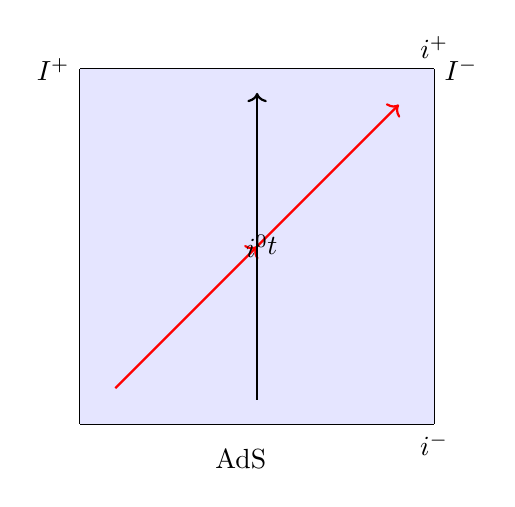
\begin{tikzpicture}[scale=1.5]
    % 绘制边界
    \draw[thick] (-1.5,-1.5) -- (-1.5,1.5) node[left] {$\mathscr{I}^+$};
    \draw[thick] (1.5,-1.5) -- (1.5,1.5) node[right] {$\mathscr{I}^-$};
    \draw[thick] (-1.5,1.5) -- (1.5,1.5) node[above] {$i^+$};
    \draw[thick] (-1.5,-1.5) -- (1.5,-1.5) node[below] {$i^-$};
    
    % 绘制 AdS 内部
    \fill[blue!10] (-1.5,-1.5) rectangle (1.5,1.5);
    
    % 绘制类光测地线
    \draw[red, thick, ->] (-1.2,-1.2) -- (0,0);
    \draw[red, thick, ->] (0,0) -- (1.2,1.2);
    
    % 标注
    \node at (0,0) {$i^0$};
    \node at (0,-1.8) {AdS 体空间};
    
    % 绘制时间方向
    \draw[->, thick] (0,-1.3) -- (0,1.3) node[midway, right] {$t$};
\end{tikzpicture}
\caption{AdS 空间的 Penrose 图。矩形区域代表整个 AdS 空间。左右边界 $\mathscr{I}^\pm$ 是类时的，上下顶点 $i^\pm$ 分别是未来和过去无穷远。}
\label{fig:AdS_Penrose}
\end{figure}

\begin{remark}
AdS 空间的 Penrose 图与闵可夫斯基时空的 Penrose 图有本质区别。在闵可夫斯基时空中，类光无穷远 $\mathscr{I}^\pm$ 是类光的（45度倾斜）；而在 AdS 空间中，类光无穷远是类时的（垂直）。这意味着：
\begin{itemize}
    \item 光信号可以在有限时间内从边界传播到体空间内部
    \item AdS 空间没有真正的"无穷远"——边界是有限距离的
    \item 这为 AdS/CFT 对偶提供了自然的边界条件
\end{itemize}
\end{remark}

\begin{remark}[AdS 的边界条件 \cite{Witten1998}]
Witten 在 \cite{Witten1998} 中详细讨论了 AdS 空间的边界条件问题。由于 AdS 的边界是类时的（而非类光的），边界上的场需要满足特定的边界条件才能唯一确定体空间中的解。对于质量为 $m$ 的标量场，边界上的渐近行为为：
\begin{equation}
    \phi(z, x) \sim z^{d-\Delta} \phi_0(x) + z^\Delta \langle \mathcal{O}(x) 
angle, \quad z \to 0,
\end{equation}
其中 $\Delta = \frac{d}{2} + \sqrt{\frac{d^2}{4} + m^2 L^2}$。Witten 指出，为了定义一个良定的变分问题，我们需要指定 $\phi_0(x)$（即 non-normalizable 模的边界值）作为边界条件 \cite{Witten1998}。这对应于在 CFT 中添加源项 $\int \phi_0 \mathcal{O}$。
\end{remark}

\begin{proof}[Penrose 图的构造]
我们来详细说明如何从全局坐标构造 Penrose 图。从全局度规出发：
\begin{equation}
    ds^2 = \frac{L^2}{\cos^2\rho}\left(-dt^2 + d\rho^2 + \sin^2\rho \, d\Omega_{d-1}^2\right),
\end{equation}
其中 $\rho \in [0, \pi/2)$，$t \in (-\infty, \infty)$。

引入新的坐标以将无穷远压缩到有限范围：
\begin{align}
    t + \rho &= \tan\left(\frac{T+R}{2}\right), \notag \\
    t - \rho &= \tan\left(\frac{T-R}{2}\right),
\end{align}
其中 $T \in (-\pi, \pi)$，$R \in [0, \pi)$。在 $(T, R)$ 坐标下，AdS 的因果结构变得完全透明：
\begin{itemize}
    \item 未来无穷远 $i^+$：$T = \pi$，$R = 0$
    \item 过去无穷远 $i^-$：$T = -\pi$，$R = 0$
    \item 空间无穷远 $i^0$：$R = \pi$，$T = 0$
    \item 类光无穷远 $\mathscr{I}^\pm$：$T = \pm(\pi - R)$
\end{itemize}
因此 Penrose 图是一个矩形，边界 $\mathscr{I}^\pm$ 是垂直的直线（类时的），这与闵可夫斯基时空（边界是倾斜的 45 度线）形成鲜明对比。
\end{proof}

\subsection{全局时间与因果性}

在全局坐标下，AdS 空间的时间坐标 $t$ 的范围是 $-\infty < t < \infty$（非紧致化版本）。由于类光无穷远是类时的，光信号可以在有限时间内从边界传播到体空间内部，然后返回边界。

考虑一个从边界点 $(t_0, r = \infty)$ 发出的类光信号。在全局坐标下，这个信号沿测地线传播，在时间 $\Delta t = \pi$ 后到达"对侧"边界。这意味着 AdS 空间的"往返时间"是有限的，为 $\pi L$（以全局时间计量）。

\subsection{庞加莱视界}

庞加莱坐标只覆盖 AdS 空间的一半。在 $z \to \infty$ 处，存在一个\textbf{庞加莱视界}（Poincaré horizon），它将庞加莱补丁与 AdS 的其他部分隔开。

\begin{remark}
庞加莱视界不是一个真正的因果视界——观察者可以穿过它。但它标志着庞加莱坐标的适用范围的边界。在 AdS/CFT 对偶中，庞加莱补丁对应于边界 CFT 定义在闵可夫斯基时空上的情况。如果需要覆盖整个 AdS 空间（例如研究全局 AdS/CFT），则需要使用全局坐标。
\end{remark}

%=============================================================================
\section{AdS 中的测地线}

测地线是弯曲时空中"直线"的推广，它描述了自由粒子在时空中运动的轨迹。在 AdS 空间中，测地线的行为对于理解全息对偶、黑洞物理和纠缠熵都很重要 \cite{Maldacena1997}。

\subsection{测地线方程}

在 AdS 空间中，测地线方程为：
\begin{equation}
    \frac{d^2 x^\mu}{d\tau^2} + \Gamma^\mu_{\rho\sigma} \frac{dx^\rho}{d\tau} \frac{dx^\sigma}{d\tau} = 0,
\end{equation}
其中 $\tau$ 是仿射参数，$\Gamma^\mu_{\rho\sigma}$ 是 Christoffel 符号。

\subsection{Christoffel 符号的推导}

在庞加莱坐标下，AdS 度规为 $ds^2 = (L^2/z^2)(-dt^2 + d\vec{x}^2 + dz^2)$。我们来详细推导 Christoffel 符号。

首先，写出度规张量的分量：
\begin{equation}
    g_{\mu\nu} = \frac{L^2}{z^2} \eta_{\mu\nu}, \quad g^{\mu\nu} = \frac{z^2}{L^2} \eta^{\mu\nu},
\end{equation}
其中 $\eta_{\mu\nu} = \text{diag}(-1, 1, \ldots, 1)$ 是闵可夫斯基度规。

Christoffel 符号的定义为：
\begin{equation}
    \Gamma^\mu_{\nu\rho} = \frac{1}{2} g^{\mu\sigma} (\partial_\nu g_{\rho\sigma} + \partial_\rho g_{\nu\sigma} - \partial_\sigma g_{\nu\rho}).
\end{equation}

由于度规只依赖于 $z$ 坐标，只有 $\partial_z g_{\mu\nu} \neq 0$。计算 $\partial_z g_{\mu\nu}$：
\begin{equation}
    \partial_z g_{\mu\nu} = \partial_z \left(\frac{L^2}{z^2} \eta_{\mu\nu}\right) = -\frac{2L^2}{z^3} \eta_{\mu\nu} = -\frac{2}{z} g_{\mu\nu}.
\end{equation}

现在计算各 Christoffel 符号。首先，当 $\mu = z$ 时：
\begin{equation}
    \Gamma^z_{\nu\rho} = \frac{1}{2} g^{zz} (\partial_\nu g_{\rho z} + \partial_\rho g_{\nu z} - \partial_z g_{\nu\rho}).
\end{equation}

对于 $\Gamma^z_{tt}$：
\begin{equation}
    \Gamma^z_{tt} = \frac{1}{2} g^{zz} (\partial_t g_{tz} + \partial_t g_{tz} - \partial_z g_{tt}) = \frac{1}{2} \cdot \frac{z^2}{L^2} \cdot \left(-\partial_z g_{tt}\right).
\end{equation}
由于 $g_{tt} = -L^2/z^2$，$\partial_z g_{tt} = 2L^2/z^3$，因此：
\begin{equation}
    \Gamma^z_{tt} = \frac{1}{2} \cdot \frac{z^2}{L^2} \cdot \left(-\frac{2L^2}{z^3}\right) = -\frac{1}{z}.
\end{equation}

对于 $\Gamma^z_{xx}$（$x$ 是任意边界空间坐标）：
\begin{equation}
    \Gamma^z_{xx} = \frac{1}{2} g^{zz} (-\partial_z g_{xx}) = \frac{1}{2} \cdot \frac{z^2}{L^2} \cdot \left(-\frac{2L^2}{z^3}\right) = -\frac{1}{z}.
\end{equation}

对于 $\Gamma^z_{zz}$：
\begin{equation}
    \Gamma^z_{zz} = \frac{1}{2} g^{zz} (\partial_z g_{zz} + \partial_z g_{zz} - \partial_z g_{zz}) = \frac{1}{2} g^{zz} \partial_z g_{zz} = \frac{1}{2} \cdot \frac{z^2}{L^2} \cdot \left(-\frac{2L^2}{z^3}\right) = -\frac{1}{z}.
\end{equation}

对于 $\Gamma^t_{tz}$：
\begin{equation}
    \Gamma^t_{tz} = \frac{1}{2} g^{tt} (\partial_t g_{zt} + \partial_z g_{tt} - \partial_t g_{tz}) = \frac{1}{2} g^{tt} \partial_z g_{tt} = \frac{1}{2} \cdot \left(-\frac{z^2}{L^2}\right) \cdot \frac{2L^2}{z^3} = -\frac{1}{z}.
\end{equation}

类似地，$\Gamma^x_{xz} = -1/z$。

\begin{remark}
所有非零的 Christoffel 符号都等于 $-1/z$，这反映了 AdS 空间的高度对称性。物理上，$-1/z$ 项对应于"引力势"的梯度：当我们向体空间内部运动（$z$ 增加）时，引力势变强，这导致测地线向体空间弯曲。
\end{remark}

\begin{example}[纯径向测地线]
考虑纯径向运动：$dt/d\tau = E$，$d\vec{x}/d\tau = 0$。测地线方程给出：
\begin{equation}
    \frac{d^2 z}{d\tau^2} - \frac{1}{z} \left(\frac{dz}{d\tau}\right)^2 + \frac{E^2}{z} = 0.
\end{equation}
令 $u = \ln z$，方程变为 $u'' + E^2 e^{-2u} = 0$，其解为：
\begin{equation}
    z(\tau) = z_0 e^{\pm E \tau / L}.
\end{equation}
正号对应于从边界向体空间运动（$z$ 增加），负号对应于从体空间向边界运动（$z$ 减小）。测地线在有限仿射参数内到达边界（$z \to 0$），但需要无穷大的仿射参数才能到达庞加莱视界（$z \to \infty$）。
\end{example}

\begin{example}[类空测地线的推导]
考虑类空测地线在 $t = \text{const}$ 超曲面上的投影。对于连接边界上两点 $(\vec{x}_1, z=0)$ 和 $(\vec{x}_2, z=0)$ 的测地线，我们来详细推导其形状。

\textbf{物理动机}：在 AdS 空间中，测地线是"最短路径"。由于 AdS 的负曲率，测地线会向体空间内部弯曲，形成一个"凹"的形状。这类似于在双曲面上，两点之间的最短路径是向内弯曲的弧线。

\textbf{步骤 1：建立测地线方程}。在 $t = \text{const}$ 超曲面上，度规为：
\begin{equation}
    ds^2 = \frac{L^2}{z^2} (dx^2 + dz^2).
\end{equation}
测地线方程为：
\begin{equation}
    \frac{d^2 z}{dx^2} - \frac{1}{z} \left(\frac{dz}{dx}\right)^2 + \frac{1}{z} = 0.
\end{equation}

\textbf{步骤 2：求解方程}。令 $z' = dz/dx$，方程变为：
\begin{equation}
    z'' - \frac{1}{z} (z')^2 + \frac{1}{z} = 0.
\end{equation}
由于方程不显含 $x$，存在守恒量：
\begin{equation}
    \mathcal{H} = z' \frac{\partial f}{\partial z'} - f = \text{const},
\end{equation}
其中 $f = \sqrt{1 + z'^2}/z$。计算得：
\begin{equation}
    \mathcal{H} = -\frac{1}{z\sqrt{1 + z'^2}} = -\frac{1}{R},
\end{equation}
其中 $R$ 是常数（半圆的半径）。

\textbf{步骤 3：求解形状}。从守恒量得到：
\begin{equation}
    1 + z'^2 = \frac{R^2}{z^2},
\end{equation}
即：
\begin{equation}
    z' = \pm \frac{\sqrt{R^2 - z^2}}{z}.
\end{equation}
积分得到：
\begin{equation}
    z(x) = \sqrt{R^2 - (x - x_0)^2},
\end{equation}
其中 $x_0$ 是积分常数。这是一个半圆，其最大深度为 $z_* = R$。

\textbf{物理意义}：类空测地线是半圆，这反映了 AdS 空间的负曲率。在闵可夫斯基时空中，类空测地线是直线；在 AdS 空间中，类空测地线是半圆。这个结果在全息纠缠熵的计算中起着核心作用。
\end{example}

\begin{figure}[htbp]
\centering
\begin{tikzpicture}[scale=1.2]
    % 绘制 AdS 边界
    \draw[thick, blue] (-4,0) -- (4,0) node[right] {边界};
    
    % 绘制类空测地线（半圆）
    \draw[thick, red, domain=-2:2, samples=100] plot (\x, {sqrt(4 - \x*\x)});
    
    % 标注端点
    \fill[red] (-2,0) circle (0.1) node[below] {$\vec{x}_1$};
    \fill[red] (2,0) circle (0.1) node[below] {$\vec{x}_2$};
    
    % 标注最大深度
    \draw[dashed, gray] (0,2) -- (0,0);
    \node at (0.5,2) {$z_* = R$};
    
    % 标注距离
    \draw[<->] (-2,-0.5) -- (2,-0.5);
    \node at (0,-0.8) {$L = 2R$};
    
    % 绘制径向方向
    \draw[->, gray] (3,0) -- (3,-2);
    \node at (3.3,-1) {$z$};
\end{tikzpicture}
\caption{AdS 空间中的类空测地线。连接边界上两点的测地线是半圆，其最大深度为 $z_* = R = L/2$。}
\label{fig:geodesic}
\end{figure}

\begin{figure}[htbp]
\centering
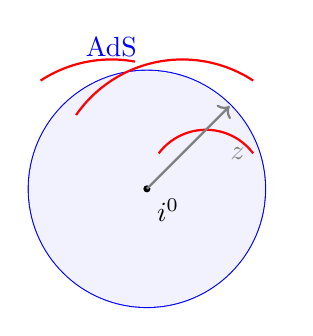
\begin{tikzpicture}[scale=1.5]
    % 绘制 Poincaré 圆盘
    \draw[thick, blue] (0,0) circle (1);
    
    % 填充
    \fill[blue!5] (0,0) circle (1);
    
    % 绘制几条测地线（半圆）
    \draw[thick, red, domain=0.1:0.9, samples=50] plot (\x, {sqrt(0.25 - (\x-0.5)*(\x-0.5))});
    \draw[thick, red, domain=-0.6:0.9, samples=50] plot (\x, {sqrt(1.2 - (\x-0.3)*(\x-0.3))});
    \draw[thick, red, domain=-0.9:-0.1, samples=50] plot (\x, {sqrt(1.2 - (\x+0.3)*(\x+0.3))});
    
    % 标注边界
    \node[blue] at (0,1.2) {AdS 边界（共形边界）};
    
    % 标注中心
    \fill[black] (0,0) circle (0.03) node[below right] {$i^0$};
    
    % 标注测地线
    \node[red] at (0.8,0.8) {测地线};
    
    % 绘制径向方向
    \draw[->, gray, thick] (0,0) -- (0.7,0.7);
    \node[gray] at (0.9,0.3) {$z$（径向）};
\end{tikzpicture}
\caption{Poincaré 圆盘模型（AdS$_2$）。蓝色圆是共形边界，红色曲线是测地线。在 AdS 空间中，测地线是与边界正交的圆弧 \cite{Witten1998}。}
\label{fig:Poincare_disk}
\end{figure}

\subsection{测地线距离与两点函数}

在 AdS/CFT 对偶中，边界 CFT 的两点关联函数可以通过体空间中的传播子来计算 \cite{Witten1998}。对于标量场，传播子正比于 $e^{-\Delta \sigma/L}$，其中 $\Delta$ 是算符的共形维数，$\sigma$ 是测地线距离。在两点距离 $|x_{12}|$ 远大于 $z$ 的极限下：
\begin{equation}
    \langle \mathcal{O}(x_1) \mathcal{O}(x_2) \rangle \sim \frac{1}{|x_{12}|^{2\Delta}},
\end{equation}
这与 CFT 中由共形对称性固定的形式一致 \cite{Maldacena1997}。

%=============================================================================
\section{AdS 中的波动方程}

在 AdS 空间中，场的行为由 Klein-Gordon 方程（对于标量场）或更一般的波动方程描述。理解这些方程的解对于计算 AdS/CFT 中的关联函数至关重要 \cite{Witten1998}。

\subsection{Klein-Gordon 方程的推导}

在 AdS 空间中，场的行为由 Klein-Gordon 方程（对于标量场）或更一般的波动方程描述。理解这些方程的解对于计算 AdS/CFT 中的关联函数至关重要 \cite{Aharony1999}。

\textbf{物理动机}：在 AdS/CFT 对偶中，边界 CFT 的算符对应于体空间中的场。为了计算关联函数，我们需要求解体空间中的波动方程。Klein-Gordon 方程是最简单的波动方程，它描述了无自旋的标量场在弯曲时空中的传播。

\textbf{从作用量出发}：标量场 $\phi$ 的作用量为：
\begin{equation}
    S = -\frac{1}{2} \int d^{d+1}x \sqrt{-g} \left( g^{\mu\nu} \partial_\mu \phi \partial_\nu \phi + m^2 \phi^2 \right).
\end{equation}
第一项是动能项，第二项是质量项。对 $\phi$ 变分，得到运动方程：
\begin{equation}
    \frac{1}{\sqrt{-g}} \partial_\mu \left( \sqrt{-g} g^{\mu\nu} \partial_\nu \phi \right) - m^2 \phi = 0.
\end{equation}
这就是弯曲时空中的 Klein-Gordon 方程：
\begin{equation}
    (\Box - m^2) \phi = 0,
\end{equation}
其中 $\Box = \frac{1}{\sqrt{-g}} \partial_\mu (\sqrt{-g} g^{\mu\nu} \partial_\nu)$ 是达朗贝尔算符。

\textbf{在庞加莱坐标下}：AdS 度规为 $ds^2 = (L^2/z^2)(-dt^2 + d\vec{x}^2 + dz^2)$，因此：
\begin{equation}
    g_{\mu\nu} = \frac{L^2}{z^2} \eta_{\mu\nu}, \quad g^{\mu\nu} = \frac{z^2}{L^2} \eta^{\mu\nu}, \quad \sqrt{-g} = \left(\frac{L}{z}\right)^{d+1}.
\end{equation}
代入 Klein-Gordon 方程：
\begin{equation}
    \frac{z^{d+1}}{L^{d+1}} \partial_\mu \left( \frac{L^{d+1}}{z^{d+1}} \frac{z^2}{L^2} \eta^{\mu\nu} \partial_\nu \phi \right) - m^2 \phi = 0.
\end{equation}
简化后得到：
\begin{equation}
    \frac{z^{d+1}}{L^2} \partial_z \left(\frac{L^2}{z^{d+1}} \partial_z \phi\right) + \frac{z^2}{L^2} \eta^{\mu\nu} \partial_\mu \partial_\nu \phi - m^2 \phi = 0.
\end{equation}

\subsection{分离变量与径向方程}

\textbf{物理动机}：由于边界是平移不变的，我们可以将场分解为不同动量的模式。这类似于量子力学中的分离变量：将多维问题分解为多个一维问题。

对方程做傅里叶变换：
\begin{equation}
    \phi(z, x) = \int \frac{d^d k}{(2\pi)^d} e^{ik \cdot x} \phi_k(z),
\end{equation}
其中 $k^2 = -\omega^2 + \vec{k}^2$。代入方程，得到径向部分满足：
\begin{equation}
    \left[\frac{1}{z^{d+1}} \partial_z \left(z^{d+1} \partial_z\right) + \frac{k^2}{z^2} - \frac{m^2 L^2}{z^2}\right] \phi_k = 0.
    \label{eq:AdS_radial}
\end{equation}
这个方程描述了场在径向方向上的行为，是 AdS/CFT 计算的核心方程。

\subsection{边界行为与质量-维数关系的推导}

\textbf{物理动机}：在边界 $z \to 0$ 附近，场的行为决定了边界 CFT 中对应算符的性质。我们需要确定场在边界附近的渐近行为，以及这如何与算符的共形维数相关联。

在边界 $z \to 0$ 附近，方程 \eqref{eq:AdS_radial} 的主导项为：
\begin{equation}
    \frac{1}{z^{d+1}} \partial_z \left(z^{d+1} \partial_z \phi_k\right) - \frac{m^2 L^2}{z^2} \phi_k \approx 0.
\end{equation}
这是一个 Euler 方程，其解具有幂律形式 $\phi_k \sim z^\alpha$。代入方程：
\begin{equation}
    \frac{1}{z^{d+1}} \partial_z \left(z^{d+1} \alpha z^{\alpha-1}\right) - \frac{m^2 L^2}{z^2} z^\alpha = 0.
\end{equation}
计算第一项：
\begin{equation}
    \frac{1}{z^{d+1}} \partial_z \left(\alpha z^{d+\alpha}\right) = \frac{1}{z^{d+1}} \cdot \alpha(d+\alpha) z^{d+\alpha-1} = \frac{\alpha(d+\alpha)}{z^2} z^\alpha.
\end{equation}
因此方程变为：
\begin{equation}
    \frac{\alpha(d+\alpha)}{z^2} z^\alpha - \frac{m^2 L^2}{z^2} z^\alpha = 0.
\end{equation}
约去 $z^\alpha/z^2$，得到特征方程：
\begin{equation}
    \alpha(d+\alpha) = m^2 L^2.
\end{equation}
定义 $\Delta = d + \alpha$（即 $\alpha = \Delta - d$），则方程变为：
\begin{equation}
    (\Delta - d) \Delta = m^2 L^2,
\end{equation}
即：
\begin{equation}
    \Delta(\Delta - d) = m^2 L^2.
    \label{eq:mass_dimension}
\end{equation}
这就是\textbf{质量-维数关系}（mass-dimension relation）！

\textbf{求解}：方程 \eqref{eq:mass_dimension} 是 $\Delta$ 的二次方程：
\begin{equation}
    \Delta^2 - d\Delta - m^2 L^2 = 0.
\end{equation}
其解为：
\begin{equation}
    \Delta_\pm = \frac{d}{2} \pm \sqrt{\frac{d^2}{4} + m^2 L^2}.
\end{equation}
两个解分别对应于场在边界附近的两种行为：
\begin{itemize}
    \item $\Delta_+$（大根）：$\phi \sim z^{\Delta_+ - d} = z^{\sqrt{d^2/4 + m^2 L^2} - d/2}$，当 $z \to 0$ 时衰减（如果 $\Delta_+ > d$）
    \item $\Delta_-$（小根）：$\phi \sim z^{\Delta_- - d} = z^{-\sqrt{d^2/4 + m^2 L^2} - d/2}$，当 $z \to 0$ 时发散
\end{itemize}

因此，场在边界附近的渐近行为为：
\begin{equation}
    \phi_k(z) \sim A(k) z^{d-\Delta} + B(k) z^\Delta,
\end{equation}
其中 $\Delta = \Delta_+$，$A(k)$ 对应于源，$B(k)$ 对应于期望值。

\begin{theorem}[质量-维数关系]
在 AdS/CFT 对偶中，体空间中质量为 $m$ 的标量场对应于边界 CFT 中共形维数为 $\Delta$ 的算符，两者满足：
\begin{equation}
    \Delta(\Delta - d) = m^2 L^2.
\end{equation}
其解为：
\begin{equation}
    \Delta_\pm = \frac{d}{2} \pm \sqrt{\frac{d^2}{4} + m^2 L^2}.
\end{equation}
通常选择 $\Delta = \Delta_+$ 作为物理的共形维数。
\end{theorem}

\begin{note}[物理意义]
质量-维数关系是 AdS/CFT 对偶中最重要的关系之一。它的物理意义是：
\begin{itemize}
    \item \textbf{质量越大 $\to$ 衰减越快}：质量越大的粒子，在体空间中传播时衰减越快，对应于边界 CFT 中维数越大的算符
    \item \textbf{无质量场}：当 $m^2 L^2 = 0$ 时，$\Delta = d$ 或 $\Delta = 0$，对应于无质量场（如规范场、应力张量）
    \item \textbf{BF 界}：当 $m^2 L^2 < 0$ 时，$\Delta$ 可能是复数，但只要满足 BF 界，$\Delta$ 仍然是实数
\end{itemize}
\end{note}

\subsection{正常izable 与 non-normalizable 模}

边界行为中的两个解具有不同的物理意义：
\begin{itemize}
    \item \textbf{Non-normalizable 模}（$z^{d-\Delta}$）：在边界上发散，对应于 CFT 中的\textbf{源}（source）。$A(k)$ 是源函数 $\phi_0(k)$。
    \item \textbf{Normalizable 模}（$z^\Delta$）：在边界上衰减，对应于 CFT 中算符的\textbf{期望值}。$B(k)$ 与 $\langle \mathcal{O}(k) \rangle$ 相关。
\end{itemize}

在 GKPW 关系中，边界条件为 $\phi \to z^{d-\Delta} \phi_0$（当 $z \to 0$），其中 $\phi_0$ 是 CFT 中的源。

\begin{remark}[GKPW 关联函数 \cite{Witten1998}]
Gubser-Klebanov-Polyakov \cite{Gubser1998} 和 Witten \cite{Witten1998} 独立地提出了 AdS/CFT 对偶中计算关联函数的基本公式（称为 GKPW 关系）。对于体空间中的标量场 $\phi$，其边界条件为 $\phi(z \to 0, x) \to z^{d-\Delta} \phi_0(x)$，其中 $\phi_0(x)$ 是边界 CFT 中算符 $\mathcal{O}(x)$ 的源。生成泛函为：
\begin{equation}
    \left\langle \exp\left(\int d^d x \, \phi_0(x) \mathcal{O}(x)\right) \right\rangle_{\rm CFT} = Z_{\rm string}[\phi \to z^{d-\Delta} \phi_0 \text{ at boundary}].
\end{equation}
在经典引力极限（$G_N \to 0$）下，弦理论的配分函数简化为 $Z_{\rm string} \approx e^{-S_{\rm on-shell}}$，因此：
\begin{equation}
    \left\langle \exp\left(\int d^d x \, \phi_0(x) \mathcal{O}(x)\right) \right\rangle_{\rm CFT} \approx e^{-S_{\rm classical}[\phi \to z^{d-\Delta} \phi_0]}.
\end{equation}
对 $\phi_0$ 求泛函导数，可以得到 CFT 中算符的关联函数。例如，两点函数为：
\begin{equation}
    \langle \mathcal{O}(x_1) \mathcal{O}(x_2) \rangle = \frac{(2\Delta - d) \Gamma(\Delta)}{\pi^{d/2} \Gamma(\Delta - d/2)} \cdot \frac{1}{|x_{12}|^{2\Delta}},
\end{equation}
这与 CFT 中由共形对称性固定的形式一致 \cite{Witten1998}。
\end{remark}

\subsection{Breitenlohner-Freedman 界}

对于 AdS 空间中的标量场，存在一个质量下界，称为\textbf{Breitenlohner-Freedman（BF）界}：
\begin{equation}
    m^2 L^2 \geq -\frac{d^2}{4}.
\end{equation}
当 $m^2 L^2 < 0$ 时，场是\textbf{快子}（tachyonic）的，但只要满足 BF 界，AdS 的负曲率可以稳定这个不稳定性。

\begin{remark}
BF 界的物理意义是：AdS 空间的负曲率提供了一个"引力势阱"，可以束缚快子场。这与闵可夫斯基时空不同——在闵可夫斯基时空中，任何负质量平方的场都是不稳定的。BF 界在 AdS/CFT 对偶中有重要的物理含义：它对应于边界 CFT 中算符维数的么正性界 \cite{Aharony1999}。
\end{remark}

\begin{proof}[BF 界的推导 \cite{Aharony1999}]
我们来证明：当 $m^2 L^2 \geq -d^2/4$ 时，标量场在 AdS 空间中是稳定的。考虑标量场的作用量：
\begin{equation}
    S = -\frac{1}{2} \int d^{d+1}x \sqrt{-g} \left( g^{\mu\nu} \partial_\mu \phi \partial_\nu \phi + m^2 \phi^2 \right).
\end{equation}
在全局坐标下，$\sqrt{-g} = (L/\cos\rho)^{d+1}$。对作用量做分部积分：
\begin{equation}
    S = -\frac{1}{2} \int d^{d+1}x \sqrt{-g} \left( -\phi \Box \phi + m^2 \phi^2 \right) + \text{边界项}.
\end{equation}
对于模式 $\phi \sim e^{-i\omega t} Y_{\ell}(\Omega) f(\rho)$，能量为 $E = \omega$。如果所有模式都有 $E^2 \geq 0$（即 $\omega$ 为实数），则系统是稳定的。

在 AdS 边界附近（$\rho \to \pi/2$），径向方程的渐近行为为 $f \sim \cos^\alpha\rho$，其中 $\alpha(\alpha-d) = m^2 L^2$。为了使作用量有下界（即能量有下界），我们需要径向方程没有负范数态。这要求：
\begin{equation}
    \alpha = \frac{d}{2} + \sqrt{\frac{d^2}{4} + m^2 L^2} \in \mathbb{R},
\end{equation}
即 $m^2 L^2 \geq -d^2/4$。当 $m^2 L^2 = -d^2/4$ 时，$\alpha = d/2$，这是临界情况。因此，BF 界为：
\begin{equation}
    m^2 L^2 \geq -\frac{d^2}{4}.
\end{equation}
\end{proof}

\subsection{精确解：AdS$_{5}$ 中的标量场}

作为具体例子，考虑 AdS$_5$（$d=4$）中的标量场。径向方程 \eqref{eq:AdS_radial} 变为：
\begin{equation}
    \left[\frac{1}{z^5} \partial_z \left(z^5 \partial_z\right) - k^2 - \frac{m^2 L^2}{z^2}\right] \phi_k = 0.
\end{equation}
令 $\phi_k(z) = z^2 f(z)$，方程变为修正的贝塞尔方程：
\begin{equation}
    z^2 f'' + z f' - \left(\Delta^2 + k^2 z^2\right) f = 0,
\end{equation}
其中 $\Delta = 2 + \sqrt{4 + m^2 L^2}$。解为：
\begin{equation}
    \phi_k(z) = z^2 \left[ A(k) K_\Delta(|k|z) + B(k) I_\Delta(|k|z) \right],
\end{equation}
其中 $K_\Delta$ 和 $I_\Delta$ 是修正的贝塞尔函数。在边界 $z \to 0$ 附近：
\begin{equation}
    \phi_k(z) \sim A(k) \Gamma(\Delta) \left(\frac{|k|z}{2}\right)^{-\Delta} 2^{\Delta-1} + B(k) \Gamma(-\Delta) \left(\frac{|k|z}{2}\right)^\Delta 2^{-\Delta-1}.
\end{equation}
这与一般分析一致：$A(k)$ 对应于源，$B(k)$ 对应于期望值。

%=============================================================================
\section{AdS 的热力学：黑洞解}

AdS 空间可以支持黑洞解。与渐近平坦时空中的黑洞不同，AdS 黑洞具有独特的热力学性质，这在 AdS/CFT 对偶中对应于边界 CFT 的热态 \cite{Hawking1983, Maldacena1997}。

\subsection{AdS-Schwarzschild 黑洞}

\begin{definition}[AdS-Schwarzschild 黑洞]
AdS$_{d+1}$ 中的 Schwarzschild 黑洞度规为：
\begin{equation}
    ds^2 = -f(r) dt^2 + \frac{dr^2}{f(r)} + r^2 d\Omega_{d-1}^2,
    \label{eq:AdS_Schwarzschild}
\end{equation}
其中：
\begin{equation}
    f(r) = 1 + \frac{r^2}{L^2} - \frac{\mu}{r^{d-2}}.
\end{equation}
参数 $\mu$ 与黑洞质量 $M$ 的关系为：
\begin{equation}
    M = \frac{(d-1) \omega_{d-1}}{16\pi G_N} \mu,
\end{equation}
其中 $\omega_{d-1} = 2\pi^{d/2}/\Gamma(d/2)$ 是单位 $(d-1)$ 维球面的面积。
\end{definition}

\begin{note}[与渐近平坦黑洞的区别]
AdS 黑洞与渐近平坦时空中的 Schwarzschild 黑洞有本质区别：
\begin{itemize}
    \item \textbf{无毛定理}：AdS 黑洞同样满足无毛定理，但其渐近行为不同
    \item \textbf{温度行为}：AdS 黑洞的温度有最小值，而渐近平坦黑洞的温度随质量减小而增大
    \item \textbf{稳定性}：AdS 黑洞是热力学稳定的，而小的渐近平坦黑洞会通过霍金辐射蒸发
\end{itemize}
\end{note}

\subsection{视界与霍金温度}

视界半径 $r_h$ 由 $f(r_h) = 0$ 确定：
\begin{equation}
    1 + \frac{r_h^2}{L^2} = \frac{\mu}{r_h^{d-2}}.
\end{equation}
对于给定的质量 $M$，这个方程可能有一个或两个解。大视界 $r_+$ 对应于黑洞，小视界 $r_-$ 对应于 Cauchy 视界。

\textbf{霍金温度}（Hawking temperature）通过表面引力 $\kappa$ 计算：
\begin{equation}
    T = \frac{\kappa}{2\pi} = \frac{f'(r_h)}{4\pi} = \frac{1}{4\pi} \left( \frac{d \, r_h}{L^2} + \frac{d-2}{r_h} \right).
    \label{eq:Hawking_T}
\end{equation}

\begin{figure}[htbp]
\centering
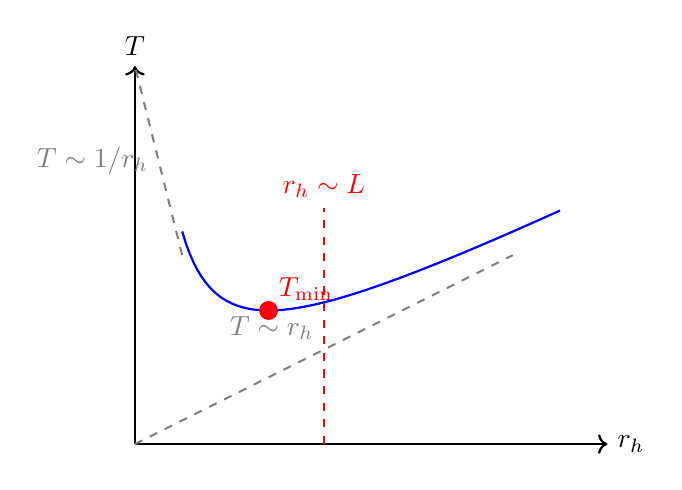
\begin{tikzpicture}[scale=1.2]
    % 绘制坐标轴
    \draw[thick, ->] (0,0) -- (5,0) node[right] {$r_h$};
    \draw[thick, ->] (0,0) -- (0,4) node[above] {$T$};
    
    % 绘制温度曲线
    \draw[thick, blue, domain=0.5:4.5, samples=100] 
        plot (\x, {0.5*\x + 1/\x});
    
    % 标注最小值
    \fill[red] (1.414, 1.414) circle (0.1) node[above right] {$T_{\min}$};
    
    % 标注渐近行为
    \draw[dashed, gray] (0,0) -- (4,2) node[midway, above left] {$T \sim r_h$};
    \draw[dashed, gray] (0.5,2) -- (0,4) node[midway, left] {$T \sim 1/r_h$};
    
    % 标注 AdS 半径
    \draw[dashed, red] (2,0) -- (2,2.5) node[above] {$r_h \sim L$};
\end{tikzpicture}
\caption{AdS 黑洞的温度 $T$ 与视界半径 $r_h$ 的关系。温度在 $r_h \sim L$ 处达到最小值 $T_{\min} \sim d/(2\pi L)$。}
\label{fig:AdS_BH_T}
\end{figure}

\begin{property}[AdS 黑洞的温度行为]
与渐近平坦时空中的 Schwarzschild 黑洞不同，AdS 黑洞的温度有最小值：
\begin{itemize}
    \item 当 $r_h \gg L$ 时，$T \approx d r_h/(4\pi L^2)$，温度与视界半径成正比
    \item 当 $r_h \ll L$ 时，$T \approx (d-2)/(4\pi r_h)$，温度与视界半径成反比
    \item 温度在 $r_h \sim L$ 处达到最小值 $T_{\min} \sim d/(2\pi L)$
\end{itemize}
\end{property}

\subsection{黑洞热力学}

AdS 黑洞具有丰富的热力学性质。我们来详细讨论这些性质。

\textbf{贝肯斯坦-霍金熵}：黑洞的熵由贝肯斯坦-霍金公式给出：
\begin{equation}
    S = \frac{A}{4G_N} = \frac{\omega_{d-1} r_h^{d-1}}{4G_N}.
\end{equation}
这个熵是广延量，与边界 CFT 的热力学熵一致。

\textbf{热力学第一定律}：AdS 黑洞的热力学量满足热力学第一定律：
\begin{equation}
    dM = T dS.
\end{equation}
将 $M$、$T$ 和 $S$ 表示为 $r_h$ 的函数，可以验证这个关系：
\begin{align}
    dM &= \frac{(d-1) \omega_{d-1}}{16\pi G_N} \left( (d-2) r_h^{d-3} + d \frac{r_h^{d-1}}{L^2} \right) dr_h, \\
    T dS &= \frac{1}{4\pi} \left( \frac{d \, r_h}{L^2} + \frac{d-2}{r_h} \right) \cdot \frac{(d-1) \omega_{d-1} r_h^{d-2}}{4G_N} dr_h,
\end{align}
两者相等。

\textbf{自由能}：黑洞的亥姆霍兹自由能为：
\begin{equation}
    F = M - TS = -\frac{\omega_{d-1} r_h^d}{16\pi G_N L^2}.
\end{equation}
在高温极限 $r_h \gg L$ 下：
\begin{equation}
    F \approx -\frac{\pi^2}{2} N^2 T^4 V,
\end{equation}
其中 $V$ 是边界体积。这与 $\mathcal{N}=4$ SYM 在强耦合极限下的自由能一致。

\textbf{霍金-佩奇相变}：在 AdS 空间中，热 AdS（thermal AdS）和 AdS 黑洞之间发生相变，称为\textbf{霍金-佩奇相变}（Hawking-Page transition）\cite{Hawking1983}。当温度 $T > T_c$ 时，AdS 黑洞是稳定的状态；当 $T < T_c$ 时，热 AdS 是稳定的状态。临界温度为：
\begin{equation}
    T_c = \frac{d}{2\pi L}.
\end{equation}
在临界温度处，自由能连续，但其一阶导数（熵）不连续，因此这是一阶相变。

\begin{remark}
霍金-佩奇相变在 AdS/CFT 对偶中对应于边界 CFT 中的\textbf{禁闭/解禁闭相变}（confinement/deconfinement transition）\cite{Witten1998b}。在禁闭相（$T < T_c$）中，自由能与 $N^0$ 成正比，对应于强子相；在解禁闭相（$T > T_c$）中，自由能与 $N^2$ 成正比，对应于夸克-胶子等离子体相 \cite{Aharony1999}。这个相变是理解 QCD 相图的重要工具。
\end{remark}

\begin{remark}[AdS 黑洞与全息对偶 \cite{Aharony1999}]
AdS 黑洞在全息对偶中有深刻的物理意义 \cite{Aharony1999}：
\begin{itemize}
    \item \textbf{热态对应}：AdS 黑洞对应于边界 CFT 的热态。黑洞的温度等于 CFT 的温度，黑洞的熵等于 CFT 的热力学熵
    \item \textbf{大 $N$ 极限}：在 $N \to \infty$ 极限下，黑洞的量子涨落可以忽略，热力学量与 $N^2$ 成正比，这与 $\mathcal{N}=4$ SYM 的自由度数一致
    \item \textbf{剪切粘滞系数}：AdS 黑洞的准正则模（quasinormal modes）对应于边界 CFT 中的流体力学模式，剪切粘滞系数与熵密度之比为 $\eta/s = 1/(4\pi)$，这是一个普适的结果 \cite{Policastro2001, Kovtun2005}
\end{itemize}
\end{remark}

%=============================================================================
\section{AdS 空间的直观理解}

为了帮助读者建立对 AdS 空间的直观理解，我们总结几个关键的物理图像。

\subsection{几何直观}

\textbf{"碗"状几何}：AdS 空间可以被想象为一个"碗"状的几何。边界在碗的边缘（$z = 0$），而碗的底部（$z = \infty$）是 AdS 的"中心"。径向坐标 $z$ 对应于从边界到体空间的"深度"。

这个"碗"的比喻有一个重要的特点：碗的"体积"在边界附近发散。这是因为度规因子 $L^2/z^2$ 在 $z \to 0$ 时发散。这意味着 AdS 空间在边界附近有无限大的"体积"，这与 CFT 中 UV 发散的物理图像一致。

\textbf{径向方向作为能量尺度}：在 AdS/CFT 对偶中，径向坐标 $z$ 可以被理解为能量尺度的倒数：
\begin{equation}
    z \sim \frac{1}{\mu},
\end{equation}
其中 $\mu$ 是能量尺度。边界 $z \to 0$ 对应于紫外（UV，高能），体空间内部 $z \to \infty$ 对应于红外（IR，低能）。这个对应关系是 AdS/CFT 中重整化群流的几何实现。

\textbf{AdS 与双曲空间}：AdS 空间与双曲空间（hyperbolic space）有密切联系。AdS$_{d+1}$ 的空间部分是 $d$ 维双曲空间 $H^d$。双曲空间是常负曲率的黎曼流形，其度规为：
\begin{equation}
    ds^2_{H^d} = \frac{L^2}{z^2} \left( d\vec{x}^2 + dz^2 \right).
\end{equation}
这恰好是 AdS 度规的空间部分。双曲空间的等距群是 $SO(1,d)$，这对应于 AdS 空间等距群 $SO(2,d)$ 的子群。

%=============================================================================
\section{AdS 空间的物理意义与应用}

AdS 空间不仅仅是一个数学构造，它在理论物理学中有着深刻的物理意义和广泛的应用。我们来详细讨论这些方面 \cite{Maldacena1997}。

\subsection{AdS 空间与量子引力}

AdS 空间在量子引力研究中扮演着核心角色。这是因为：
\begin{itemize}
    \item \textbf{负曲率的稳定性}：AdS 空间的负曲率提供了一个"引力势阱"，可以束缚场的涨落。这使得 AdS 空间在量子引力中是稳定的，而渐近平坦时空可能不是。
    \item \textbf{边界条件}：AdS 空间具有类时的边界，这为定义量子引力理论提供了自然的边界条件。我们可以指定边界上的场值，这对应于在 CFT 中添加源。
    \item \textbf{全息性质}：AdS 空间的全息性质（即体空间的物理可以由边界理论描述）为量子引力提供了一个非微扰的定义 \cite{Maldacena1997}。
\end{itemize}

\begin{remark}[AdS/CFT 字典 \cite{Maldacena1997}]
AdS/CFT 对偶建立了一套精确的对应关系（称为"字典"）\cite{Maldacena1997}：
\begin{itemize}
    \item \textbf{态的对应}：CFT 的真空态对应于纯 AdS 空间；CFT 的热态对应于 AdS 黑洞 \cite{Hawking1983}
    \item \textbf{算符的对应}：CFT 中的算符 $\mathcal{O}$ 对应于体空间中的场 $\phi$，两者通过质量-维数关系 $m^2 L^2 = \Delta(\Delta-d)$ 相联系
    \item \textbf{对称性的对应}：CFT 的共形群 $SO(2,d)$ 对应于 AdS 的等距群 $SO(2,d)$
    \item \textbf{耦合常数的对应}：CFT 的 't Hooft 耦合 $\lambda = g_{\rm YM}^2 N$ 对应于弦理论参数 $L^4/\alpha'^2$
    \item \textbf{自由度的对应}：CFT 的中心荷 $c \sim N^2$ 对应于引力理论中 $L^{d-1}/(8\pi G_N)$
\end{itemize}
这个字典使得我们可以通过计算体空间中的经典引力问题来得到强耦合 CFT 的非微扰信息。
\end{remark}

\begin{figure}[htbp]
\centering
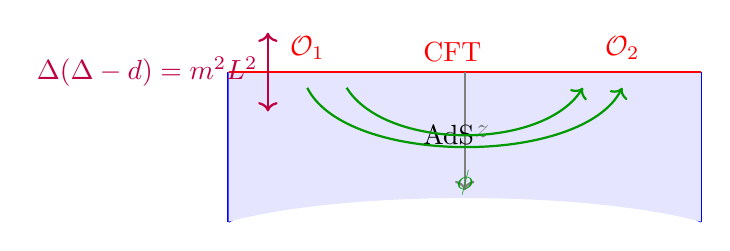
\begin{tikzpicture}[scale=1.0]
    % 绘制 AdS 体空间（碗状）
    \draw[thick, blue, domain=-3:3, samples=100] plot (\x, {-0.1*\x*\x + 3});
    \draw[thick, blue] (-3,2.1) -- (-3,4);
    \draw[thick, blue] (3,2.1) -- (3,4);
    \draw[thick, blue] (-3,4) -- (3,4);
    
    % 填充
    \fill[blue!10] (-3,2.1) .. controls (-1.5,2.5) and (1.5,2.5) .. (3,2.1) -- (3,4) -- (-3,4) -- cycle;
    
    % 标注边界
    \draw[thick, red] (-3,4) -- (3,4) node[midway, above] {CFT 边界};
    
    % 标注径向方向
    \draw[->, thick, gray] (0,4) -- (0,2.5) node[midway, right] {$z$};
    
    % 标注体空间
    \node at (0,3.2) {AdS 体空间};
    
    % 绘制场线
    \draw[->, green!60!black, thick] (-1.5,3.8) .. controls (-1,3) and (1,3) .. (1.5,3.8);
    \draw[->, green!60!black, thick] (-2,3.8) .. controls (-1.5,2.8) and (1.5,2.8) .. (2,3.8);
    
    % 标注场
    \node[green!60!black] at (0,2.6) {$\phi$};
    
    % 标注算符
    \node[red] at (-2,4.3) {$\mathcal{O}_1$};
    \node[red] at (2,4.3) {$\mathcal{O}_2$};
    
    % 标注对应关系
    \draw[<->, thick, purple] (-2.5,3.5) -- (-2.5,4.5);
    \node[purple, left] at (-2.5,4) {$\Delta(\Delta-d)=m^2L^2$};
\end{tikzpicture}
\caption{AdS/CFT 对偶的示意图。体空间中的标量场 $\phi$（绿色）对应于边界 CFT 中的算符 $\mathcal{O}$（红色），两者通过质量-维数关系联系 \cite{Maldacena1997}。}
\label{fig:AdS_CFT_dictionary}
\end{figure}

\subsection{AdS 空间与黑洞物理}

AdS 空间中的黑洞物理与渐近平坦时空中的黑洞物理有本质区别：
\begin{itemize}
    \item \textbf{热力学稳定性}：AdS 黑洞是热力学稳定的，而小的渐近平坦黑洞会通过霍金辐射蒸发 \cite{Hawking1975}。这是因为 AdS 空间的"盒子"效应限制了辐射的逃逸。
    \item \textbf{霍金-佩奇相变}：在 AdS 空间中，热 AdS 和 AdS 黑洞之间发生相变，这对应于边界 CFT 中的禁闭/解禁闭相变 \cite{Witten1998b}。这个相变是理解 QCD 相图的重要工具。
    \item \textbf{黑洞信息悖论}：AdS/CFT 对偶为黑洞信息悖论提供了新的视角。由于边界 CFT 是幺正的，黑洞蒸发过程必须保持信息守恒 \cite{Maldacena1997}。
\end{itemize}

\subsection{AdS 空间与凝聚态物理}

AdS 空间在凝聚态物理中也有重要应用：
\begin{itemize}
    \item \textbf{全息超导体}：通过在 AdS 黑洞背景中引入复标量场，可以模拟超导相变 \cite{Hartnoll2007}。当温度低于临界温度时，标量场凝聚，破坏 $U(1)$ 对称性，系统进入超导相。
    \item \textbf{全息非费米液体}：AdS/CFT 可以描述具有非费米液体行为的强耦合系统 \cite{Liu2006}。这些系统无法用传统的朗道费米液体理论描述。
    \item \textbf{全息量子临界点}：AdS/CFT 可以描述量子相变的临界行为 \cite{Hartnoll2009}。量子临界点的临界指数可以通过求解体空间中的场方程得到。
\end{itemize}

\subsection{AdS 空间与宇宙学}

虽然 AdS 空间不是我们宇宙的好的近似（我们的宇宙具有正宇宙学常数），但它在宇宙学研究中也有应用：
\begin{itemize}
    \item \textbf{AdS/CFT 与宇宙学}：AdS/CFT 对偶的思想可以推广到宇宙学设置。例如，de Sitter/CFT 对偶试图为具有正宇宙学常数的时空建立全息描述 \cite{Maldacena1998}。
    \item \textbf{暴胀模型}：某些暴胀模型可以在 AdS 空间中实现。AdS 的负曲率可以驱动宇宙的加速膨胀。
    \item \textbf{暗能量}：AdS/CFT 对偶为理解暗能量提供了新的视角。暗能量可能与真空能量有关，而 AdS/CFT 对偶可以帮助我们理解真空能量的性质。
\end{itemize}

\begin{remark}[大 $N$ 极限与 $1/N$ 展开 \cite{Aharony1999}]
AdS/CFT 对偶的一个重要方面是它在大 $N$ 极限下的行为 \cite{Aharony1999}。对于 $SU(N)$ 规范理论：
\begin{itemize}
    \item \textbf{领头阶}（$N \to \infty$，$\lambda$ 固定）：规范理论的关联函数由平面图（planar diagrams）主导，对应于体空间中的经典引力
    \item \textbf{弦修正}（$1/\alpha'$ 展开）：对应于规范理论中的 $\alpha'$ 修正，即高导数算符的贡献
    \item \textbf{量子修正}（$G_N$ 展开，即 $1/N^2$ 展开）：对应于体空间中的弦圈图，即规范理论中的非平面图贡献
\end{itemize}
$1/N$ 展开的拓扑展开性质使得 AdS/CFT 对偶具有深刻的数学结构：规范理论的微扰展开按照 Feynman 图的亏格（genus）分类，这与弦理论的弦耦合常数 $g_s \sim 1/N$ 的展开一致。
\end{remark}

\subsection{AdS 空间的历史}

AdS 空间的历史可以追溯到 19 世纪：
\begin{itemize}
    \item \textbf{1883 年}：Wilhelm Killing 在研究非欧几里得几何时，首次发现了 AdS 空间。
    \item \textbf{1917 年}：爱因斯坦在研究宇宙学时，考虑了具有负宇宙学常数的时空。
    \item \textbf{1983 年}：Hawking 和 Page 发现了 AdS 黑洞的热力学性质，这为后来的 AdS/CFT 对偶奠定了基础。
    \item \textbf{1997 年}：Maldacena 提出了 AdS/CFT 对偶，将 AdS 空间与共形场论联系起来 \cite{Maldacena1997}。这是理论物理学中最深刻的发现之一。
    \item \textbf{1998 年}：Gubser-Klebanov-Polyakov \cite{Gubser1998} 和 Witten \cite{Witten1998} 独立地给出了 AdS/CFT 对偶中计算关联函数的具体公式（GKPW 关系）。
    \item \textbf{1999 年}：Aharony、Gubser、Maldacena、Ooguri 和 Oz 发表了关于 AdS/CFT 对偶的综合性综述 \cite{Aharony1999}，系统地总结了大 $N$ 规范理论与弦理论的对偶关系。
\end{itemize}

\section{小结}

在本节中，我们系统地介绍了反德西特空间的几何性质 \cite{Aharony1999}：
\begin{itemize}
    \item AdS 空间是具有常负曲率的最大对称时空，可以通过嵌入在 $\mathbb{R}^{2,d}$ 中的超曲面定义
    \item AdS 空间有多种坐标系：全局坐标覆盖整个空间，庞加莱坐标覆盖一半，Fefferman-Graham 坐标适用于全息重整化 \cite{Witten1998}
    \item AdS 空间的等距群 $SO(2,d)$ 与 $d$ 维共形群同构，这是 AdS/CFT 对偶的对称性基础 \cite{Maldacena1997}
    \item AdS 空间的因果结构独特：类光无穷远是类时的，光信号可以在有限时间内往返边界 \cite{Witten1998}
    \item 测地线在 AdS 空间中的行为为全息纠缠熵的计算提供了基础
    \item Klein-Gordon 方程的解具有边界行为 $z^{d-\Delta}$ 和 $z^\Delta$，分别对应于源和期望值 \cite{Witten1998}
    \item AdS 黑洞具有有限温度和熵，霍金-佩奇相变对应于禁闭/解禁闭相变 \cite{Hawking1983, Witten1998b}
    \item AdS 空间在量子引力、黑洞物理、凝聚态物理和宇宙学中都有重要应用
\end{itemize}
这些几何性质为理解 AdS/CFT 对偶提供了坚实的基础。在下一节中，我们将介绍共形场论的基本概念，这是 AdS/CFT 对偶中边界理论的基础 \cite{Maldacena1997}。


\chapter{共形场论 (Conformal Field Theory)}

%=============================================================================

共形场论（conformal field theory, CFT）是具有共形对称性的量子场论。共形对称性是比庞加莱对称性（Poincaré symmetry）更大的对称性群，它包含标度变换（scale transformation）和特殊共形变换（special conformal transformation）。在 AdS/CFT 对偶中，边界理论通常是一个共形场论 \cite{Maldacena1997}。共形对称性对关联函数施加了很强的约束，使得我们可以精确计算许多物理量 \cite{Aharony1999}。本节的内容为理解 AdS/CFT 对偶提供必要的基础。

\begin{note}[CFT 的物理应用]
CFT 在现代理论物理学中有着广泛的应用：
\begin{itemize}
    \item \textbf{临界现象}：连续相变的临界点处，关联长度发散，系统表现出尺度不变性，临界行为可以用 CFT 描述
    \item \textbf{弦理论}：弦的世界面理论是一个 2 维 CFT \cite{Polchinski1998}
    \item \textbf{凝聚态物理}：量子霍尔效应、自旋链、拓扑相变等都与 CFT 密切相关
    \item \textbf{AdS/CFT 对偶}：边界理论是一个 CFT，共形对称性是 AdS/CFT 的对称性基础 \cite{Maldacena1997}
\end{itemize}
\end{note}

%=============================================================================
\section{共形变换}

\begin{definition}[共形变换]
共形变换（conformal transformation）是保持角度不变的坐标变换。更精确地说，共形变换是保持度规形式不变，只改变其整体标度的变换：
\begin{equation}
    \bar{g}_{\mu\nu}(x') = \Omega^2(x) g_{\mu\nu}(x),
\end{equation}
其中 $\Omega(x) > 0$ 是标度因子（scale factor），它可以依赖于时空坐标。
\end{definition}

\begin{note}[直观理解]
想象一张橡皮膜，你可以在上面画图。共形变换就像是拉伸这张膜，但要求保持所有角度不变。这意味着你可以改变图形的大小，但不能改变它的形状。例如，一个正方形可以变成一个更大的正方形，但不能变成长方形。
\end{note}

\begin{remark}[因果结构]
共形变换保持两个曲线之间的角度不变，但可以改变长度的标度。这意味着共形变换保持因果结构（causal structure）不变，因为光锥（light cone）由角度定义。这是一个非常重要的物理性质：共形变换不改变物理系统的因果关系。
\end{remark}

\begin{theorem}[共形群与 AdS 等距群]
在 $d$ 维闵可夫斯基空间中，共形变换群是 $SO(2, d)$，这恰好等于 AdS$_{d+1}$ 空间的等距群（isometry group）。这是 AdS/CFT 对偶的对称性基础 \cite{Maldacena1997}。
\end{theorem}

\subsection{无穷小共形变换与共形 Killing 方程的推导}

\begin{note}[物理动机]
我们希望找到所有保持角度不变的无穷小坐标变换。这些变换构成了共形群，是 CFT 的对称性基础。在物理上，这意味着系统没有内在的特征长度尺度，这正是临界现象的特征。
\end{note}

\begin{theorem}[共形 Killing 方程的推导]
考虑无穷小坐标变换 $x^\mu \to x'^\mu = x^\mu + \epsilon^\mu(x)$。度规的变化为：
\begin{equation}
    g_{\mu\nu}(x) \to g'_{\mu\nu}(x') = g_{\mu\nu}(x) - \partial_\mu \epsilon_\nu - \partial_\nu \epsilon_\mu.
\end{equation}
共形变换要求度规只改变整体标度：
\begin{equation}
    g'_{\mu\nu}(x') = \Omega^2(x) g_{\mu\nu}(x) \approx (1 + 2\omega(x)) g_{\mu\nu}(x),
\end{equation}
其中 $\omega(x)$ 是无穷小标度因子。因此：
\begin{equation}
    \partial_\mu \epsilon_\nu + \partial_\nu \epsilon_\mu = 2\omega(x) \eta_{\mu\nu}.
    \label{eq:conformal_Killing_1}
\end{equation}
\end{theorem}

\begin{proof}[确定 $\omega(x)$ 的值]
对 \eqref{eq:conformal_Killing_1} 取迹（乘以 $\eta^{\mu\nu}$）：
\begin{equation}
    \eta^{\mu\nu} (\partial_\mu \epsilon_\nu + \partial_\nu \epsilon_\mu) = 2\omega(x) \eta^{\mu\nu} \eta_{\mu\nu} = 2\omega(x) d.
\end{equation}
左边为 $2\partial \cdot \epsilon$，因此：
\begin{equation}
    \omega(x) = \frac{1}{d} \partial \cdot \epsilon.
\end{equation}
代回 \eqref{eq:conformal_Killing_1}，得到\textbf{共形 Killing 方程}：
\begin{equation}
    \partial_\mu \epsilon_\nu + \partial_\nu \epsilon_\mu = \frac{2}{d} (\partial \cdot \epsilon) \eta_{\mu\nu}.
    \label{eq:conformal_Killing}
\end{equation}
满足这个方程的矢量场 $\epsilon^\mu$ 称为\textbf{共形 Killing 矢量}（conformal Killing vector）。
\end{proof}

\begin{remark}
共形 Killing 方程 \eqref{eq:conformal_Killing} 的物理意义是：无穷小坐标变换保持角度不变，当且仅当度规的变化是整体标度变换。这比一般的等距变换（保持度规不变）更宽松，因此共形群比等距群更大。
\end{remark}

\begin{figure}[htbp]
\centering
\begin{tikzpicture}[scale=1.0]
    % 平移
    \draw[thick, blue, ->] (0,0) -- (1.5,0) node[midway, below] {$a^\mu$};
    \draw[thick, blue] (0,0) rectangle (1,1);
    \draw[thick, blue, dashed] (1.5,0) rectangle (2.5,1);
    \node at (0.5, 1.3) {\small 原始图形};
    \node at (2.0, 1.3) {\small 平移};
    % 旋转
    \draw[thick, red] (4,0) rectangle (5,1);
    \draw[thick, red, dashed, rotate=30] (4,0) rectangle (5,1);
    \node at (4.5, 1.3) {\small 旋转};
    % 标度
    \draw[thick, green!60!black] (7,0) rectangle (8,1);
    \draw[thick, green!60!black, dashed] (7,0) rectangle (8.5,1.5);
    \node at (7.5, 1.8) {\small 标度变换};
\end{tikzpicture}
\caption{共形变换的直观理解：平移保持图形不变，旋转保持角度和距离不变，标度变换改变大小但保持角度不变。}
\label{fig:conformal_transformations}
\end{figure}

\subsection{共形 Killing 方程的解}

\begin{theorem}[共形 Killing 方程的一般解]
共形 Killing 方程 \eqref{eq:conformal_Killing} 的一般解为：
\begin{equation}
    \epsilon^\mu(x) = a^\mu + {\omega^\mu}_\nu x^\nu + \lambda x^\mu + (b \cdot x) x^\mu - \frac{1}{2} b^\mu x^2,
\end{equation}
其中：
\begin{itemize}
    \item $a^\mu$：平移参数（$d$ 个）
    \item $\omega_{\mu\nu} = -\omega_{\nu\mu}$：旋转参数（$d(d-1)/2$ 个）
    \item $\lambda$：标度变换参数（1 个）
    \item $b^\mu$：特殊共形变换参数（$d$ 个）
\end{itemize}
\end{theorem}

\begin{proof}[参数计数]
总参数数目为 $d + d(d-1)/2 + 1 + d = d(d+3)/2 + 1$。去掉整体标度（它不改变物理），独立参数数目为 $d(d+3)/2$，这正是共形群 $SO(2,d)$ 的维数：
\begin{equation}
    \dim SO(2,d) = \frac{(d+2)(d+1)}{2} - 1 = \frac{d(d+3)}{2}.
\end{equation}
对于 $d=4$，共形群有 15 个生成元。这比庞加莱群的 10 个生成元多出 5 个，多出的就是标度变换和 4 个特殊共形变换。
\end{proof}

\begin{example}[各变换的物理意义]
\begin{itemize}
    \item $a^\mu$：将整个系统平移 $a^\mu$，不改变任何物理性质
    \item $\omega_{\mu\nu}$：将系统旋转，保持距离不变
    \item $\lambda$：将系统整体放大或缩小，但保持形状不变
    \item $b^\mu$：特殊共形变换，可以理解为先做反演变换，然后平移，然后再做反演变换
\end{itemize}
\end{example}

\subsection{有限共形变换}

从无穷小变换可以积分得到有限变换。四种基本的有限共形变换为：

\begin{definition}[平移]
\begin{equation}
    x'^\mu = x^\mu + a^\mu.
\end{equation}
\end{definition}

\begin{definition}[旋转]
\begin{equation}
    x'^\mu = {\Lambda^\mu}_\nu x^\nu, \quad \Lambda^T \eta \Lambda = \eta.
\end{equation}
\end{definition}

\begin{definition}[标度变换]
\begin{equation}
    x'^\mu = \lambda x^\mu, \quad \lambda > 0.
\end{equation}
标度变换将所有长度缩放 $\lambda$ 倍，但保持角度不变。
\end{definition}

\begin{definition}[特殊共形变换]
\begin{equation}
    x'^\mu = \frac{x^\mu - b^\mu x^2}{1 - 2b \cdot x + b^2 x^2}.
\end{equation}
\end{definition}

\begin{proof}[特殊共形变换的分解]
特殊共形变换可以分解为三步：
\begin{enumerate}
    \item 反演变换 $x^\mu \to x^\mu/x^2$
    \item 平移 $x^\mu \to x^\mu - b^\mu$
    \item 再次反演变换 $x^\mu \to x^\mu/x^2$
\end{enumerate}
验证：设 $I(x^\mu) = x^\mu/x^2$，则 $I(I(x^\mu)) = x^\mu$。组合 $I \circ T_{-b} \circ I$ 给出：
\begin{equation}
    x^\mu \xrightarrow{I} \frac{x^\mu}{x^2} \xrightarrow{T_{-b}} \frac{x^\mu}{x^2} - b^\mu \xrightarrow{I} \frac{x^\mu - b^\mu x^2}{|x - b x^2|^2} = \frac{x^\mu - b^\mu x^2}{1 - 2b \cdot x + b^2 x^2}.
\end{equation}
\end{proof}

\subsection{反演变换与物理意义}

\begin{definition}[反演变换]
反演变换（inversion）是特殊共形变换的基本组成部分：
\begin{equation}
    x^\mu \to \frac{x^\mu}{x^2}.
\end{equation}
反演变换将靠近原点的点映射到远离原点的点，反之亦然。在反演变换下，度规变换为：
\begin{equation}
    g_{\mu\nu} \to \frac{1}{(x^2)^2} g_{\mu\nu}.
\end{equation}
因此反演变换是共形变换，标度因子为 $\Omega(x) = 1/x^2$。
\end{definition}

\begin{remark}[共形不变性与标度不变性]
共形不变性是比标度不变性更强的对称性。标度不变性只要求系统在整体缩放下不变，而共形不变性还要求在特殊共形变换下不变。在大多数情况下，标度不变性自动蕴含共形不变性，但也存在反例。
\end{remark}

%=============================================================================
\section{共形代数}

\begin{definition}[共形变换的生成元]
共形变换的生成元（generators of conformal transformations）为：
\begin{itemize}
    \item \textbf{平移}：$P_\mu = -i\partial_\mu$。平移生成元将系统在时空中整体移动，不改变系统的任何内部性质。
    \item \textbf{旋转}：$M_{\mu\nu} = i(x_\mu \partial_\nu - x_\nu \partial_\mu)$。旋转生成元将系统绕某个轴旋转，保持系统的距离不变。
    \item \textbf{标度变换}：$D = -ix^\mu \partial_\mu$。标度变换将系统整体放大或缩小，但保持形状不变。这是共形对称性特有的生成元。
    \item \textbf{特殊共形变换}：$K_\mu = i(x^2 \partial_\mu - 2x_\mu x^\nu \partial_\nu)$。特殊共形变换是一种更复杂的变换，它可以被理解为先做反演变换（inversion），然后平移，然后再做反演变换。
\end{itemize}
\end{definition}

\begin{theorem}[共形代数]
这些生成元满足李代数（Lie algebra）：
\begin{align}
    [D, P_\mu] &= iP_\mu, \label{eq:conf_alg_1}\\
    [D, K_\mu] &= -iK_\mu, \label{eq:conf_alg_2}\\
    [K_\mu, P_\nu] &= 2i(\eta_{\mu\nu}D - M_{\mu\nu}), \label{eq:conf_alg_3}\\
    [M_{\mu\nu}, P_\rho] &= i(\eta_{\nu\rho}P_\mu - \eta_{\mu\rho}P_\nu), \label{eq:conf_alg_4}\\
    [M_{\mu\nu}, K_\rho] &= i(\eta_{\nu\rho}K_\mu - \eta_{\mu\rho}K_\nu), \label{eq:conf_alg_5}\\
    [M_{\mu\nu}, M_{\rho\sigma}] &= i(\eta_{\nu\rho}M_{\mu\sigma} - \eta_{\mu\rho}M_{\nu\sigma} - \eta_{\nu\sigma}M_{\mu\rho} + \eta_{\mu\sigma}M_{\nu\rho}). \label{eq:conf_alg_6}
\end{align}
\end{theorem}

\begin{proof}[对易关系 $[D, P_\mu] = iP_\mu$ 的推导]
将生成元作用于测试函数 $f(x)$：
\begin{align}
    [D, P_\mu] f(x) &= (-ix^\nu \partial_\nu)(-i\partial_\mu) f - (-i\partial_\mu)(-ix^\nu \partial_\nu) f \notag \\
    &= -x^\nu \partial_\nu \partial_\mu f + \partial_\mu (x^\nu \partial_\nu f) \notag \\
    &= -x^\nu \partial_\nu \partial_\mu f + \delta_\mu^\nu \partial_\nu f + x^\nu \partial_\mu \partial_\nu f \notag \\
    &= \partial_\mu f = iP_\mu f.
\end{align}
因此 $[D, P_\mu] = iP_\mu$。
\end{proof}

\begin{proof}[对易关系 $[K_\mu, P_\nu]$ 的推导]
计算 $[K_\mu, P_\nu]$ 作用于 $f(x)$：
\begin{align}
    [K_\mu, P_\nu] f &= i(x^2 \partial_\mu - 2x_\mu x^\rho \partial_\rho)(-i\partial_\nu) f - (-i\partial_\nu) i(x^2 \partial_\mu - 2x_\mu x^\rho \partial_\rho) f \notag \\
    &= (x^2 \partial_\mu - 2x_\mu x^\rho \partial_\rho)\partial_\nu f - \partial_\nu(x^2 \partial_\mu f - 2x_\mu x^\rho \partial_\rho f).
\end{align}
展开第二项：
\begin{align}
    \partial_\nu(x^2 \partial_\mu f) &= 2x_\nu \partial_\mu f + x^2 \partial_\nu \partial_\mu f, \\
    \partial_\nu(2x_\mu x^\rho \partial_\rho f) &= 2\eta_{\mu\nu} x^\rho \partial_\rho f + 2x_\mu \partial_\nu f + 2x_\mu x^\rho \partial_\rho \partial_\nu f.
\end{align}
合并后得到：
\begin{equation}
    [K_\mu, P_\nu] f = -2x_\nu \partial_\mu f + 2\eta_{\mu\nu} x^\rho \partial_\rho f - 2x_\mu \partial_\nu f.
\end{equation}
注意到 $2\eta_{\mu\nu} x^\rho \partial_\rho f = -2i\eta_{\mu\nu} D f$，而 $-2(x_\nu \partial_\mu - x_\mu \partial_\nu) f = -2i M_{\mu\nu} f$，因此：
\begin{equation}
    [K_\mu, P_\nu] = 2i(\eta_{\mu\nu} D - M_{\mu\nu}).
\end{equation}
\end{proof}

\begin{note}[对易关系的物理意义]
这些对易关系告诉我们，标度变换 $D$ 可以将平移生成元 $P_\mu$ "放大"或"缩小"。这意味着在标度变换下，动量的量纲会发生变化。这正是共形维数的物理来源。
\end{note}

\subsection{共形代数的结构}

\begin{theorem}[$SO(2,d)$ 的实现]
共形代数 \eqref{eq:conf_alg_1}-\eqref{eq:conf_alg_6} 可以用更统一的方式理解。定义：
\begin{equation}
    J_{AB} = \{M_{\mu\nu}, P_\mu, K_\mu, D\}, \quad A, B = -1, 0, 1, \ldots, d,
\end{equation}
则共形代数可以写成：
\begin{equation}
    [J_{AB}, J_{CD}] = i(\eta_{AD}J_{BC} - \eta_{AC}J_{BD} + \eta_{BC}J_{AD} - \eta_{BD}J_{AC}),
\end{equation}
其中 $\eta_{AB} = \text{diag}(-1,-1,+1,\ldots,+1)$。这正是 $SO(2,d)$ 的李代数。
\end{theorem}

\begin{property}[生成元的对应关系]
\begin{align}
    M_{\mu\nu} &= J_{\mu\nu}, & P_\mu &= J_{-1,\mu} + J_{0,\mu}, \notag \\
    K_\mu &= J_{-1,\mu} - J_{0,\mu}, & D &= J_{-1,0}.
\end{align}
\end{property}

\subsection{与 AdS 等距群的对应}

\begin{theorem}[共形代数与 AdS 等距代数的同构]
共形代数与 AdS$_{d+1}$ 的等距代数完全相同。这个对应关系是 AdS/CFT 对偶的对称性基础 \cite{Maldacena1997}：
\begin{center}
\begin{tabular}{|c|c|}
\hline
\textbf{CFT 共形变换} & \textbf{AdS 等距变换} \\
\hline
平移 $P_\mu$ & AdS 中的平移 \\
旋转 $M_{\mu\nu}$ & AdS 中的旋转 \\
标度变换 $D$ & AdS 中的径向平移 \\
特殊共形变换 $K_\mu$ & AdS 中的特殊等距 \\
\hline
\end{tabular}
\end{center}
\end{theorem}

%=============================================================================
\section{共形维数和初级算符}

\begin{definition}[共形维数]
在标度变换 $x \to \lambda x$ 下，算符 $\mathcal{O}(x)$ 的变换规律为：
\begin{equation}
    \mathcal{O}(x) \to \lambda^{-\Delta} \mathcal{O}(\lambda x),
\end{equation}
其中 $\Delta$ 称为共形维数（conformal dimension）。共形维数度量算符在标度变换下的"权重"：当我们将系统放大 $\lambda$ 倍时，算符的值会乘以 $\lambda^{-\Delta}$。
\end{definition}

\subsection{初级算符的定义}

\begin{definition}[初级算符]
初级算符（primary operator）是共形群的"最低权态"，它满足：
\begin{equation}
    [K_\mu, \mathcal{O}(x)] = 0, \quad [D, \mathcal{O}(x)] = -i\Delta \mathcal{O}(x).
\end{equation}
\end{definition}

\begin{note}[物理动机]
在量子场论中，所有其他态都可以通过对基本粒子作用动量算符得到。类似地，在 CFT 中，所有其他算符都可以通过对初级算符作用平移生成元 $P_\mu$ 得到。这些通过对初级算符作用平移生成元得到的算符称为后裔算符（descendant operator），例如 $\partial_\mu \mathcal{O}(x)$ 是 $\mathcal{O}(x)$ 的后裔算符。
\end{note}

\subsection{初级算符的变换规律}

在一般的共形变换下，初级算符的变换规律为：

\begin{property}[平移变换]
\begin{equation}
    e^{ia^\mu P_\mu} \mathcal{O}(x) e^{-ia^\mu P_\mu} = \mathcal{O}(x+a).
\end{equation}
\end{property}

\begin{property}[标度变换]
\begin{equation}
    e^{i\lambda D} \mathcal{O}(x) e^{-i\lambda D} = e^{-\lambda \Delta} \mathcal{O}(e^\lambda x).
\end{equation}
\end{property}

\begin{property}[旋转变换]
\begin{equation}
    e^{i\frac{1}{2}\omega^{\mu\nu}M_{\mu\nu}} \mathcal{O}(x) e^{-i\frac{1}{2}\omega^{\mu\nu}M_{\mu\nu}} = {R^{-1}}^\Delta_\Delta \mathcal{O}(R x),
\end{equation}
其中 $R$ 是旋转矩阵，对于标量算符 ${R^{-1}}^\Delta_\Delta = 1$。
\end{property}

\begin{property}[特殊共形变换]
\begin{equation}
    e^{ib^\mu K_\mu} \mathcal{O}(x) e^{-ib^\mu K_\mu} = |1 - 2b \cdot x + b^2 x^2|^\Delta \mathcal{O}\left(\frac{x - b x^2}{1 - 2b \cdot x + b^2 x^2}\right).
\end{equation}
\end{property}

\subsection{不同场的共形维数}

\begin{note}[物理动机]
在 CFT 中，不同类型的场具有不同的共形维数。这些共形维数可以通过对称性分析来确定。共形维数与场的质量量纲密切相关，在 AdS/CFT 对偶中，它与体空间中对应场的质量直接相关。
\end{note}

\begin{property}[基本场的共形维数]
在 $d$ 维 CFT 中，基本场的共形维数为：
\begin{itemize}
    \item \textbf{标量场} $\phi(x)$：$\Delta = (d-2)/2$
    \item \textbf{费米子场} $\psi(x)$：$\Delta = (d-1)/2$
    \item \textbf{守恒流} $J_\mu(x)$：$\Delta = d-1$
    \item \textbf{应力张量} $T_{\mu\nu}(x)$：$\Delta = d$
\end{itemize}
\end{property}

\begin{example}[4 维 CFT 中的共形维数]
在 4 维 CFT 中（$d=4$）：
\begin{itemize}
    \item 标量场：$\Delta = 1$，这意味着标量场在标度变换下像长度的倒数一样变换
    \item 费米子场：$\Delta = 3/2$，费米子场的共形维数比标量场大，这意味着费米子场在短距离下衰减得更快
    \item 守恒流：$\Delta = 3$，守恒流的共形维数与其守恒律密切相关
    \item 应力张量：$\Delta = 4$，应力张量是 CFT 中最重要的算符之一，因为它与能量-动量守恒相关
\end{itemize}
\end{example}

\begin{note}[共形维数的物理意义]
共形维数 $\Delta$ 度量了算符在标度变换下的"权重"：
\begin{itemize}
    \item 当我们将系统放大 $\lambda$ 倍时，算符的值会乘以 $\lambda^{-\Delta}$
    \item 这类似于物理学中的量纲分析：能量的量纲是 1，长度的量纲是 -1
    \item 在 AdS/CFT 对偶中，共形维数与体空间中对应场的质量相关：$\Delta(\Delta-d) = m^2 L^2$ \cite{Gubser1998}
\end{itemize}
\end{note}

\subsection{共形维数与自旋}

\begin{definition}[幺正性界]
对于具有自旋的算符，共形维数和自旋共同确定了算符在共形变换下的行为。在 $d$ 维空间中，算符由两个量子数标记：共形维数 $\Delta$ 和自旋 $l$（或更一般地，由 $SO(d)$ 的表示标记）。

对于标量算符（$l = 0$），共形维数满足幺正性界：
\begin{equation}
    \Delta \geq \frac{d-2}{2}.
\end{equation}
对于守恒流（$l = 1$），$\Delta = d-1$。对于应力张量（$l = 2$），$\Delta = d$。
\end{definition}

\begin{remark}
当幺正性界的等号成立时，对应的算符是守恒的。例如，$\Delta = d-1$ 对应守恒流，$\Delta = d$ 对应守恒应力张量。这些守恒算符在 AdS/CFT 对偶中对应于规范场和引力场 \cite{Witten1998}。
\end{remark}

\subsection{后裔算符}

\begin{definition}[后裔算符]
后裔算符是通过对初级算符作用平移生成元得到的算符。对于标量初级算符 $\mathcal{O}(x)$，后裔算符为：
\begin{align}
    \text{一级后裔：} & \quad \partial_\mu \mathcal{O}(x), \quad \Delta_{\text{desc}} = \Delta + 1, \notag \\
    \text{二级后裔：} & \quad \partial_\mu \partial_\nu \mathcal{O}(x), \quad \Delta_{\text{desc}} = \Delta + 2, \notag \\
    \text{一般后裔：} & \quad \partial_{\mu_1} \cdots \partial_{\mu_n} \mathcal{O}(x), \quad \Delta_{\text{desc}} = \Delta + n.
\end{align}
\end{definition}

\begin{remark}
后裔算符不是独立的算符——它们可以通过初级算符和共形代数来表示。在 CFT 的希尔伯特空间中，后裔算符构成"共形家族"的一部分。
\end{remark}

%=============================================================================
\section{共形对称性对关联函数的约束}

共形对称性对关联函数施加很强的约束，使得我们可以精确确定低点关联函数的形式。这是 CFT 最强大的性质之一：即使我们不知道理论的详细动力学，共形对称性也能告诉我们很多信息。

\subsection{一点函数的约束}

\begin{theorem}[一点函数为零]
对于非平庸的初级算符，一点函数必须为零：
\begin{equation}
    \langle \mathcal{O}(x) \rangle = 0.
\end{equation}
\end{theorem}

\begin{proof}
在标度变换下，一点函数变换为：
\begin{equation}
    \langle \mathcal{O}(x) \rangle \to \lambda^{-\Delta} \langle \mathcal{O}(\lambda x) \rangle.
\end{equation}
如果 $\langle \mathcal{O}(x) \rangle = c \neq 0$（常数），则 $c = \lambda^{-\Delta} c$，这对 $\Delta \neq 0$ 矛盾。因此 $c = 0$。
\end{proof}

\begin{remark}
对于恒等算符 $\mathbf{1}$（$\Delta = 0$），一点函数 $\langle \mathbf{1} \rangle = 1$ 是非零的。这是唯一一个具有非零一点函数的初级算符。
\end{remark}

\subsection{两点函数的详细推导}

\begin{note}[物理动机]
在 CFT 中，两点函数 $\langle \mathcal{O}(x) \mathcal{O}(y) \rangle$ 描述了两个算符之间的关联。由于 CFT 没有特征长度尺度，关联函数只能以幂律形式衰减，而不是指数形式（指数衰减对应于有质量粒子，而 CFT 中的粒子是无质量的）。
\end{note}

\begin{theorem}[两点函数的形式]
共形对称性完全确定两点函数的形式（除了归一化常数）：
\begin{equation}
    \langle \mathcal{O}_1(x) \mathcal{O}_2(y) \rangle = \frac{C_{\mathcal{O}_1\mathcal{O}_2} \delta_{\Delta_1, \Delta_2}}{|x - y|^{2\Delta}}.
\end{equation}
\end{theorem}

\begin{proof}[详细推导]
考虑两点函数 $\langle \mathcal{O}_1(x) \mathcal{O}_2(y) \rangle$。我们要求这个函数在所有共形变换下不变。

\textbf{步骤 1：平移不变性}。在平移变换 $x \to x + a$，$y \to y + a$ 下，两点函数不变：
\begin{equation}
    \langle \mathcal{O}_1(x) \mathcal{O}_2(y) \rangle = \langle \mathcal{O}_1(x+a) \mathcal{O}_2(y+a) \rangle.
\end{equation}
这意味着两点函数只能依赖于坐标差 $x - y$：
\begin{equation}
    \langle \mathcal{O}_1(x) \mathcal{O}_2(y) \rangle = f(x - y).
\end{equation}

\textbf{步骤 2：旋转不变性}。在旋转变换 $x \to Rx$，$y \to Ry$ 下，两点函数不变：
\begin{equation}
    \langle \mathcal{O}_1(x) \mathcal{O}_2(y) \rangle = \langle \mathcal{O}_1(Rx) \mathcal{O}_2(Ry) \rangle.
\end{equation}
这意味着 $f(x - y)$ 只能依赖于 $|x - y|$（旋转不变量）：
\begin{equation}
    \langle \mathcal{O}_1(x) \mathcal{O}_2(y) \rangle = g(|x - y|).
\end{equation}

\textbf{步骤 3：标度不变性}。在标度变换 $x \to \lambda x$，$y \to \lambda y$ 下：
\begin{equation}
    \langle \mathcal{O}_1(x) \mathcal{O}_2(y) \rangle = \lambda^{-\Delta_1 - \Delta_2} \langle \mathcal{O}_1(\lambda x) \mathcal{O}_2(\lambda y) \rangle.
\end{equation}
这意味着：
\begin{equation}
    g(|x - y|) = \lambda^{-\Delta_1 - \Delta_2} g(\lambda |x - y|).
\end{equation}
令 $r = |x-y|$，上式对任意 $\lambda$ 成立。令 $\lambda = 1/r$，得 $g(r) = r^{\Delta_1+\Delta_2} g(1)$，即：
\begin{equation}
    g(r) = \frac{C}{r^{\Delta_1 + \Delta_2}}.
\end{equation}

\textbf{步骤 4：算符的归一化}。对于相同的算符 $\mathcal{O}_1 = \mathcal{O}_2 = \mathcal{O}$，$\Delta_1 = \Delta_2 = \Delta$：
\begin{equation}
    \langle \mathcal{O}(x) \mathcal{O}(y) \rangle = \frac{C_{\mathcal{O}\mathcal{O}}}{|x - y|^{2\Delta}}.
\end{equation}
\end{proof}

\begin{figure}[htbp]
\centering
\begin{tikzpicture}[scale=1.2]
    % 绘制坐标轴
    \draw[thick, ->] (0,0) -- (5,0) node[right] {$|x - y|$};
    \draw[thick, ->] (0,0) -- (0,4) node[above] {$\langle \mathcal{O}(x) \mathcal{O}(y) \rangle$};
    
    % 绘制两点函数
    \draw[thick, blue, domain=0.5:4.5, samples=100] 
        plot (\x, {3/\x^2});
    
    % 标注幂律行为
    \node at (3,3) {$\sim 1/|x-y|^{2\Delta}$};
    
    % 标注共形维数
    \draw[dashed, red] (0,0) -- (4,2) node[midway, above left] {$\Delta$ 越大，衰减越快};
\end{tikzpicture}
\caption{CFT 中两点函数的幂律行为。关联函数以幂律形式衰减，衰减的快慢由共形维数 $\Delta$ 决定。}
\label{fig:two_point}
\end{figure}

\begin{note}[两点函数的物理意义]
两点函数的幂律形式 $\sim 1/|x-y|^{2\Delta}$ 反映了 CFT 中没有特征长度尺度：
\begin{itemize}
    \item \textbf{无特征长度}：CFT 中没有内在的长度尺度，所有长度都是等价的。这导致关联函数以幂律形式衰减，而不是指数形式。
    \item \textbf{共形维数}：$\Delta$ 越大，衰减越快。这意味着高维算符在短距离下衰减得更快。
    \item \textbf{正交性}：两点函数只在两个算符具有相同共形维数时才不为零。这意味着在 CFT 中，不同共形维数的算符是"正交"的。
\end{itemize}
\end{note}

\subsection{三点函数的详细推导}

\begin{note}[物理动机]
三点函数描述了三个算符之间的关联。在微扰理论中，三点函数对应于相互作用顶点。在 CFT 中，三点函数完全由共形对称性确定，唯一的自由度是 OPE 系数 $C_{123}$，它包含了理论的非平庸信息。
\end{note}

\begin{theorem}[三点函数的形式]
共形对称性完全确定三点函数的形式（除了 OPE 系数）：
\begin{equation}
    \langle \mathcal{O}_1(x) \mathcal{O}_2(y) \mathcal{O}_3(z) \rangle = \frac{C_{123}}{|x - y|^{\Delta_1 + \Delta_2 - \Delta_3} |y - z|^{\Delta_2 + \Delta_3 - \Delta_1} |x - z|^{\Delta_3 + \Delta_1 - \Delta_2}}.
\end{equation}
\end{theorem}

\begin{proof}[详细推导]
考虑三点函数 $\langle \mathcal{O}_1(x) \mathcal{O}_2(y) \mathcal{O}_3(z) \rangle$。

\textbf{步骤 1：平移不变性}。三点函数只能依赖于坐标差：
\begin{equation}
    \langle \mathcal{O}_1(x) \mathcal{O}_2(y) \mathcal{O}_3(z) \rangle = f(x - y, y - z).
\end{equation}

\textbf{步骤 2：旋转不变性}。$f$ 只能依赖于旋转不变量：
\begin{equation}
    |x - y|, \quad |y - z|, \quad |x - z|.
\end{equation}

\textbf{步骤 3：标度不变性}。在标度变换下：
\begin{equation}
    \langle \mathcal{O}_1(x) \mathcal{O}_2(y) \mathcal{O}_3(z) \rangle = \lambda^{-\Delta_1 - \Delta_2 - \Delta_3} \langle \mathcal{O}_1(\lambda x) \mathcal{O}_2(\lambda y) \mathcal{O}_3(\lambda z) \rangle.
\end{equation}
这意味着 $f$ 必须具有以下形式：
\begin{equation}
    f = \frac{h(\text{角度})}{|x - y|^{\alpha} |y - z|^{\beta} |x - z|^{\gamma}},
\end{equation}
其中 $\alpha + \beta + \gamma = \Delta_1 + \Delta_2 + \Delta_3$。

\textbf{步骤 4：特殊共形不变性}。特殊共形变换对三点函数施加了更强的约束。通过要求三点函数在特殊共形变换下不变，可以唯一地确定各幂次：
\begin{align}
    \alpha &= \Delta_1 + \Delta_2 - \Delta_3, \\
    \beta &= \Delta_2 + \Delta_3 - \Delta_1, \\
    \gamma &= \Delta_3 + \Delta_1 - \Delta_2.
\end{align}
\end{proof}

\begin{remark}
三点函数的形式完全由共形对称性确定，唯一的自由度是 OPE 系数 $C_{123}$。这意味着，如果我们知道所有 OPE 系数，我们就完全知道了 CFT。OPE 系数是 CFT 的"耦合常数"，它们决定了不同算符之间的相互作用强度。
\end{remark}

\subsection{四点函数与共形块}

\begin{definition}[共形不变量]
共形对称性不能完全确定四点函数及更高点函数的形式，但可以将其写成共形块（conformal block）的展开。定义共形不变量（conformal cross-ratios）：
\begin{equation}
    u = \frac{x_{12}^2 x_{34}^2}{x_{13}^2 x_{24}^2}, \quad v = \frac{x_{14}^2 x_{23}^2}{x_{13}^2 x_{24}^2}.
\end{equation}
共形不变量 $u$ 和 $v$ 在共形变换下保持不变，它们完全确定了四个点的"形状"，与它们的绝对位置和大小无关。
\end{definition}

\begin{theorem}[共形块展开]
四点函数可以展开为：
\begin{equation}
    \langle \mathcal{O}_1(x_1) \mathcal{O}_2(x_2) \mathcal{O}_3(x_3) \mathcal{O}_4(x_4) \rangle = \sum_{\mathcal{O}} C_{12\mathcal{O}} C_{34\mathcal{O}} G_{\Delta, l}(u, v),
\end{equation}
其中 $G_{\Delta, l}(u, v)$ 是共形块 \cite{Aharony1999}。
\end{theorem}

\begin{note}[物理解释]
共形块展开类似于量子力学中的分波展开（partial wave expansion）。在散射理论中，我们可以将散射振幅展开为不同角动量的贡献之和。类似地，在 CFT 中，我们可以将四点函数展开为不同"共形自旋"的贡献之和。
\end{note}

\begin{remark}
四点函数包含了 CFT 的完整动力学信息。OPE 系数 $C_{ij}^k$ 和共形维数 $\Delta_k$ 完全确定了四点函数，因此也完全确定了 CFT。这些数据称为 CFT 的\textbf{共形数据}（conformal data）。
\end{remark}

%=============================================================================
\section{共形 Ward 恒等式}

共形对称性导致了关联函数满足一系列约束条件，称为共形 Ward 恒等式。这些恒等式将守恒律与关联函数的对称性联系起来。

\begin{theorem}[平移 Ward 恒等式]
平移不变性要求：
\begin{equation}
    \sum_{i=1}^n \frac{\partial}{\partial x_i^\mu} \langle \mathcal{O}_1(x_1) \cdots \mathcal{O}_n(x_n) \rangle = 0.
\end{equation}
这意味着关联函数只能依赖于坐标差 $x_i - x_j$。
\end{theorem}

\begin{theorem}[旋转 Ward 恒等式]
旋转不变性要求：
\begin{equation}
    \sum_{i=1}^n \left( x_i^\mu \frac{\partial}{\partial x_i^\nu} - x_i^\nu \frac{\partial}{\partial x_i^\mu} \right) \langle \mathcal{O}_1(x_1) \cdots \mathcal{O}_n(x_n) \rangle = \text{自旋贡献}.
\end{equation}
\end{theorem}

\begin{theorem}[标度 Ward 恒等式]
标度不变性要求：
\begin{equation}
    \sum_{i=1}^n \left( x_i^\mu \frac{\partial}{\partial x_i^\mu} + \Delta_i \right) \langle \mathcal{O}_1(x_1) \cdots \mathcal{O}_n(x_n) \rangle = 0.
\end{equation}
这个方程表明，关联函数的标度维数必须等于各算符共形维数之和。
\end{theorem}

\begin{theorem}[特殊共形 Ward 恒等式]
特殊共形不变性要求：
\begin{equation}
    \sum_{i=1}^n \left( 2x_i^\mu (x_i \cdot \partial_i) - x_i^2 \partial_i^\mu + 2\Delta_i x_i^\mu \right) \langle \mathcal{O}_1(x_1) \cdots \mathcal{O}_n(x_n) \rangle = 0.
\end{equation}
这个方程是最强的约束，它将关联函数的形式几乎完全固定。
\end{theorem}

\begin{example}[两点函数的 Ward 恒等式验证]
对于两点函数 $\langle \mathcal{O}(x) \mathcal{O}(y) \rangle = C/|x-y|^{2\Delta}$，验证标度 Ward 恒等式：
\begin{equation}
    \left( x^\mu \partial_\mu + y^\mu \partial_\mu + 2\Delta \right) \frac{C}{|x-y|^{2\Delta}}.
\end{equation}
由于 $|x-y|^{2\Delta}$ 在标度变换 $x \to \lambda x$, $y \to \lambda y$ 下获得因子 $\lambda^{2\Delta}$，而算符获得因子 $\lambda^{-2\Delta}$，总效果为零。
\end{example}

%=============================================================================
\section{共形代数和表示理论}

共形群的表示理论是理解 CFT 的基础，它告诉我们 CFT 的希尔伯特空间是如何组织的。

在 $d$ 维欧几里得空间中，共形代数同构于 $SO(d+1,1)$ 的李代数。在 $d$ 维闵可夫斯基空间中，共形代数同构于 $SO(2,d)$ 的李代数。

\begin{definition}[共形家族]
CFT 的希尔伯特空间可以分解为共形群的最高权表示（highest weight representation）。每个最高权表示由一个初级算符 $\mathcal{O}$ 标记，包含该初级算符及其所有后裔算符。最高权表示可以理解为"粒子多重态"：在粒子物理学中，一个粒子多重态包含具有不同自旋投影的粒子；类似地，在 CFT 中，一个共形家族（conformal family）包含具有不同导数的算符。
\end{definition}

\begin{example}[标量初级算符的共形家族]
考虑一个标量初级算符 $\mathcal{O}(x)$，其共形维数为 $\Delta$。它的共形家族包含：
\begin{itemize}
    \item 初级算符：$\mathcal{O}(x)$，共形维数 $\Delta$
    \item 一级后裔：$\partial_\mu \mathcal{O}(x)$，共形维数 $\Delta + 1$
    \item 二级后裔：$\partial_\mu \partial_\nu \mathcal{O}(x)$，共形维数 $\Delta + 2$
    \item 以此类推...
\end{itemize}
\end{example}

\begin{figure}[htbp]
\centering
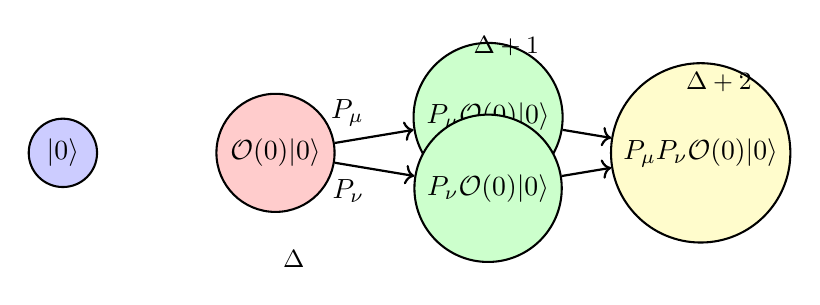
\begin{tikzpicture}[scale=0.9]
    % 算符-态对应
    \node[draw, circle, fill=blue!20] (vac) at (0,0) {$|0\rangle$};
    \node[draw, circle, fill=red!20] (O) at (3,0) {$\mathcal{O}(0)|0\rangle$};
    \node[draw, circle, fill=green!20] (PO1) at (6,0.5) {$P_\mu \mathcal{O}(0)|0\rangle$};
    \node[draw, circle, fill=green!20] (PO2) at (6,-0.5) {$P_\nu \mathcal{O}(0)|0\rangle$};
    \node[draw, circle, fill=yellow!20] (PPO) at (9,0) {$P_\mu P_\nu \mathcal{O}(0)|0\rangle$};
    \draw[thick, ->] (O) -- (PO1) node[midway, above left] {$P_\mu$};
    \draw[thick, ->] (O) -- (PO2) node[midway, below left] {$P_\nu$};
    \draw[thick, ->] (PO1) -- (PPO);
    \draw[thick, ->] (PO2) -- (PPO);
    \node at (3, -1.5) {\small 初级算符 $\Delta$};
    \node at (6, 1.5) {\small 一级后裔 $\Delta+1$};
    \node at (9, 1.0) {\small 二级后裔 $\Delta+2$};
\end{tikzpicture}
\caption{状态-算符对应与共形家族。初级算符 $\mathcal{O}(0)$ 作用于真空态产生初级态，后裔态通过对初级态作用平移生成元 $P_\mu$ 得到。}
\label{fig:state_operator}
\end{figure}

\subsection{幺正性界}

\begin{theorem}[幺正性界]
CFT 的表示理论对共形维数施加了重要的约束。对于幺正的 CFT，初级算符的共形维数必须满足：
\begin{align}
    \text{标量算符：} & \quad \Delta \geq \frac{d-2}{2}, \\
    \text{自旋 } l \text{ 算符：} & \quad \Delta \geq d - 2 + l.
\end{align}
这些界称为\textbf{幺正性界}（unitarity bounds）。当等号成立时，对应的算符是守恒的（例如，$\Delta = d-1$ 对应守恒流，$\Delta = d$ 对应守恒应力张量）。
\end{theorem}

\begin{remark}
幺正性界在 AdS/CFT 对偶中有重要的物理意义：它们对应于体空间中场的质量界。幺正的 CFT 对应于没有 ghost 的引力理论 \cite{Gubser1998}。
\end{remark}

%=============================================================================
\section{共形异常}

共形异常（conformal anomaly）或 Weyl 异常（Weyl anomaly）是量子场论中的一个重要现象，它反映了经典对称性在量子化后的破缺。共形异常的研究始于 1980 年代，由 Zamolodchikov \cite{Zamolodchikov1986} 等人的工作奠定了基础。

\begin{definition}[共形异常]
在经典水平上，共形不变的理论具有无迹的应力张量：$T_\mu^{~\mu} = 0$。但在量子水平上，应力张量的迹不为零：
\begin{equation}
    \langle T_\mu^{~\mu} \rangle = \frac{(-1)^{d/2}}{2} A E_d + \sum_i B_i I_i + \nabla_\mu J^\mu,
\end{equation}
其中 $E_d$ 是欧拉密度（Euler density），$\int E_d = \chi$ 是欧拉示性数；$I_i$ 是 Weyl 不变量（Weyl invariants），由 Weyl 张量构造；$A$ 是 $a$-异常系数；$B_i$ 是 $b$-异常系数。
\end{definition}

\begin{note}[物理理解]
共形异常可以理解为量子涨落的效应。在经典水平上，系统是共形不变的。但在量子水平上，真空涨落会"探测"到不同的长度尺度，从而破坏共形对称性。这类似于量子力学中的反常：经典对称性在量子化后被破坏。
\end{note}

\subsection{2 维共形异常}

\begin{theorem}[2 维共形异常]
在 2 维 CFT 中，共形异常的形式特别简单：
\begin{equation}
    \langle T_\mu^{~\mu} \rangle = \frac{c}{24\pi} R,
\end{equation}
其中 $c$ 是\textbf{中心荷}（central charge），$R$ 是里奇标量。中心荷 $c$ 度量了理论的"自由度"，是 2 维 CFT 中最重要的参数 \cite{Zamolodchikov1986}。
\end{theorem}

\begin{example}[自由场的中心荷]
\begin{itemize}
    \item 自由标量场：$c = 1$
    \item 自由费米子：$c = 1/2$
    \item $\mathcal{N}=1$ 超对称 CFT：$c = 3/2$
\end{itemize}
\end{example}

\subsection{4 维共形异常}

\begin{theorem}[4 维共形异常]
在 4 维 CFT 中，共形异常的形式为：
\begin{equation}
    \langle T_\mu^{~\mu} \rangle = \frac{1}{16\pi^2} \left( c W_{\mu\nu\rho\sigma} W^{\mu\nu\rho\sigma} - a E_4 \right),
\end{equation}
其中 $W_{\mu\nu\rho\sigma}$ 是 Weyl 张量，$E_4$ 是 4 维欧拉密度，$c$ 和 $a$ 是两个独立的异常系数 \cite{Henningson1998}。
\end{theorem}

\begin{example}[自由场的异常系数]
\begin{center}
\begin{tabular}{|l|c|c|}
\hline
\textbf{场} & $a$ & $c$ \\
\hline
实标量场 & $1/360$ & $1/120$ \\
Weyl 费米子 & $11/720$ & $1/40$ \\
规范场 & $31/180$ & $1/10$ \\
\hline
\end{tabular}
\end{center}
\end{example}

\subsection{$a$-定理}

\begin{theorem}[$a$-定理]
在 4 维中，$a$-异常系数沿着重整化群流单调递减：
\begin{equation}
    a_{\rm UV} > a_{\rm IR}.
\end{equation}
这个定理称为 $a$-定理（$a$-theorem），由 Komargodski 和 Schwimmer 于 2011 年证明 \cite{Komargodski2011}，它是 2 维 $c$-定理 \cite{Zamolodchikov1986} 在 4 维的推广。
\end{theorem}

\begin{note}[物理意义]
$a$-定理告诉我们，在重整化群流中，系统的"自由度"是单调递减的：当我们从高能尺度流向低能尺度时，越来越多的自由度被"冻结"，系统的有效描述变得越来越简单。$a$-异常系数 $A$ 和 $b$-异常系数 $B_i$ 称为中心荷（central charge），它度量了理论的"自由度"。
\end{note}

%=============================================================================
\section{算符乘积展开}

算符乘积展开（operator product expansion, OPE）是 CFT 中最重要的工具之一。

\begin{definition}[算符乘积展开]
OPE 声称，两个算符的乘积可以展开为其他算符的和：
\begin{equation}
    \mathcal{O}_i(x) \mathcal{O}_j(y) = \sum_k C_{ij}^k(x-y) \mathcal{O}_k(y),
\end{equation}
其中 $C_{ij}^k(x-y)$ 是 OPE 系数，它依赖于两个算符之间的距离。
\end{definition}

\begin{note}[物理理解]
OPE 可以理解为"算符的叠加原理"：当我们把两个算符放在一起时，它们的效应可以等效地表示为其他算符的效应之和。这类似于量子力学中的态叠加原理：任何态都可以表示为基态的线性组合。
\end{note}

\begin{figure}[htbp]
\centering
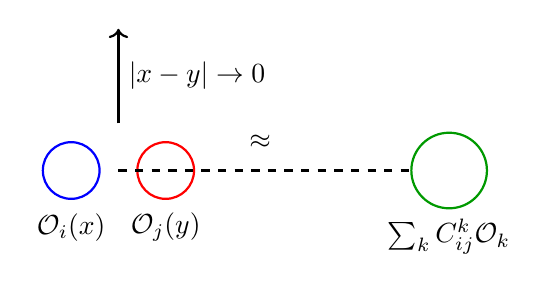
\begin{tikzpicture}[scale=1.2]
    % 两个算符靠近
    \draw[thick, blue] (0,0) circle (0.3);
    \node at (0,-0.6) {$\mathcal{O}_i(x)$};
    \draw[thick, red] (1,0) circle (0.3);
    \node at (1,-0.6) {$\mathcal{O}_j(y)$};
    \draw[thick, ->] (0.5,0.5) -- (0.5,1.5) node[midway, right] {$|x-y| \to 0$};
    % OPE 展开
    \draw[thick, green!60!black] (4,0) circle (0.4);
    \node at (4,-0.7) {$\sum_k C_{ij}^k \mathcal{O}_k$};
    \draw[thick, dashed] (0.5,0) -- (3.6,0);
    \node at (2, 0.3) {$\approx$};
\end{tikzpicture}
\caption{算符乘积展开（OPE）的示意图。当两个算符 $\mathcal{O}_i(x)$ 和 $\mathcal{O}_j(y)$ 足够接近时，它们的乘积可以展开为其他算符 $\mathcal{O}_k$ 的和。}
\label{fig:ope_diagram}
\end{figure}

\subsection{OPE 的结构}

\begin{theorem}[OPE 的共形结构]
在 CFT 中，OPE 的结构由共形对称性完全确定。对于两个标量初级算符，OPE 为：
\begin{equation}
    \mathcal{O}_i(x) \mathcal{O}_j(y) = \sum_k C_{ij}^k \frac{1}{|x-y|^{\Delta_i+\Delta_j-\Delta_k}} \left[ \mathcal{O}_k(y) + \text{后裔算符} + \cdots \right].
\end{equation}
OPE 系数 $C_{ij}^k$ 是无量纲常数，它包含了理论的非平庸信息。
\end{theorem}

\begin{remark}[OPE 的收敛性]
在 CFT 中，OPE 具有非平庸的收敛半径。当 $|x-y|$ 小于到其他算符的距离时，OPE 收敛。OPE 的收敛性告诉我们，当两个算符足够接近时，它们的行为可以用其他算符来描述。这类似于物理学中的多极展开（multipole expansion）：当距离足够远时，电荷分布可以用多极矩来描述。
\end{remark}

\subsection{OPE 系数的性质}

\begin{property}[OPE 系数的结合律]
OPE 系数 $C_{ij}^k$ 包含了理论的非平庸信息。它们满足结合律（associativity）：
\begin{equation}
    \sum_m C_{ij}^m C_{mk}^l = \sum_m C_{jk}^m C_{im}^l.
\end{equation}
结合律保证了 OPE 的一致性：无论我们以什么顺序进行 OPE，最终结果都应该相同。这类似于量子力学中的算符结合律：$(AB)C = A(BC)$。
\end{property}

\begin{property}[OPE 系数的对称性]
\begin{equation}
    C_{ij}^k = C_{ji}^k.
\end{equation}
\end{property}

\subsection{OPE 与关联函数}

\begin{theorem}[OPE 与四点函数]
OPE 系数与共形块一起决定了四点函数：
\begin{equation}
    \langle \mathcal{O}_1(x_1) \mathcal{O}_2(x_2) \mathcal{O}_3(x_3) \mathcal{O}_4(x_4) \rangle = \sum_{\mathcal{O}} C_{12\mathcal{O}} C_{34\mathcal{O}} G_{\Delta, l}(u, v).
\end{equation}
这可以理解为"通道展开"：在散射理论中，我们可以将散射振幅展开为不同通道的贡献之和（s, t, u 通道）；类似地，在 CFT 中，我们可以将四点函数展开为不同"共形通道"的贡献之和。
\end{theorem}

\subsection{共形自举}

\begin{definition}[共形自举]
OPE 的结合律对共形数据施加了很强的约束。这些约束可以用来\textbf{唯一地确定}某些 CFT 的共形数据，而不需要任何微扰计算。这种方法称为\textbf{共形自举}（conformal bootstrap）。

共形自举的基本思想是：OPE 的结合律等价于四点函数在不同通道展开的一致性条件。通过要求这些条件同时满足，可以得到共形数据的约束方程。在某些情况下，这些约束足够强，可以唯一地确定共形数据。
\end{definition}

%=============================================================================
\section{CFT 的物理意义与应用}

共形场论不仅仅是一个数学框架，它在理论物理学中有着深刻的物理意义和广泛的应用。

\subsection{CFT 与临界现象}

\begin{note}[物理动机]
CFT 最重要的物理应用之一是描述临界现象。在连续相变的临界点处，关联长度发散，系统表现出尺度不变性。此时，微观细节变得不重要，系统的临界行为可以由 CFT 描述。考虑一个铁磁体在居里温度附近的相变。当温度接近居里温度时，磁化强度的涨落变得长程相关，关联长度发散。此时，系统的临界行为不依赖于微观细节（如晶格结构），而只依赖于对称性和维度。
\end{note}

\begin{example}[临界现象的 CFT 描述]
\begin{itemize}
    \item \textbf{伊辛模型}：2 维伊辛模型的临界点由 $c = 1/2$ 的 CFT 描述
    \item \textbf{XY 模型}：2 维 XY 模型的临界点由 $c = 1$ 的 CFT 描述
    \item \textbf{海森堡模型}：2 维海森堡模型的临界点由 $c = 3/2$ 的 CFT 描述
\end{itemize}
\end{example}

\subsection{CFT 与弦理论}

\begin{note}[物理动机]
CFT 在弦理论中扮演着核心角色。弦的世界面理论是一个 2 维 CFT，这使得 CFT 成为弦理论的基础 \cite{Polchinski1998}。弦在时空中运动时，扫出一个二维曲面，称为世界面。世界面上的物理由一个 2 维量子场论描述。为了保证弦理论的自洽性（即消除共形反常），这个量子场论必须是一个 CFT。
\end{note}

\begin{example}[弦理论中的 CFT]
\begin{itemize}
    \item \textbf{玻色弦}：玻色弦的世界面理论是一个 $c = 26$ 的 CFT
    \item \textbf{超弦}：超弦的世界面理论是一个 $c = 15$ 的超对称 CFT \cite{Green1987}
    \item \textbf{弦紧致化}：弦理论的额外维度可以通过 CFT 来描述。例如，Calabi-Yau 流形上的 CFT 描述了弦的紧致化。
\end{itemize}
\end{example}

\subsection{CFT 与凝聚态物理}

\begin{example}[凝聚态物理中的 CFT]
CFT 在凝聚态物理中也有重要应用：
\begin{itemize}
    \item \textbf{量子霍尔效应}：量子霍尔效应的边缘态由手征 CFT 描述
    \item \textbf{自旋链}：1 维自旋链的低能物理由 CFT 描述
    \item \textbf{拓扑相变}：拓扑相变的临界行为由 CFT 描述
    \item \textbf{量子临界点}：量子临界点的临界行为由 CFT 描述
\end{itemize}
\end{example}

\subsection{CFT 与 AdS/CFT 对偶}

\begin{note}[CFT 在 AdS/CFT 中的角色]
CFT 是 AdS/CFT 对偶中边界理论的基础 \cite{Maldacena1997, Witten1998}。在 AdS/CFT 对偶中，边界 CFT 的物理性质对应于体空间引力理论的物理性质：
\begin{itemize}
    \item \textbf{共形对称性}：CFT 的共形对称性对应于 AdS 空间的等距对称性
    \item \textbf{算符}：CFT 的算符对应于体空间中的场
    \item \textbf{关联函数}：CFT 的关联函数对应于体空间中经典场的传播
    \item \textbf{热力学}：CFT 的热态对应于体空间中的黑洞 \cite{Witten1998b}
\end{itemize}
\end{note}

\subsection{2 维 CFT 的特殊性质}

2 维 CFT 具有特殊的性质，因为 2 维共形群是无限维的。这使得 2 维 CFT 可以被精确求解。

\begin{definition}[Virasoro 代数]
在 2 维欧几里得空间中，使用复坐标 $z = x_1 + ix_2$ 和 $\bar{z} = x_1 - ix_2$，共形变换可以分解为全纯（holomorphic）和反全纯（anti-holomorphic）两部分。

全纯共形变换的生成元为：
\begin{equation}
    L_n = -z^{n+1} \partial_z, \quad n \in \mathbb{Z}.
\end{equation}
这些生成元满足 Virasoro 代数：
\begin{equation}
    [L_m, L_n] = (m-n) L_{m+n} + \frac{c}{12} m(m^2-1) \delta_{m+n, 0},
\end{equation}
其中 $c$ 是中心荷。类似地，反全纯部分有生成元 $\bar{L}_n$ 和中心荷 $\bar{c}$。
\end{definition}

\begin{remark}
Virasoro 代数是 2 维共形代数的无限维推广。中心荷 $c$ 的出现是量子效应——在经典水平上，$c = 0$。中心荷度量了 Virasoro 代数的"中心扩张"，它在 2 维 CFT 中扮演着核心角色 \cite{Zamolodchikov1986}。
\end{remark}

\begin{proof}[Virasoro 代数中心扩展的推导]
考虑量子修正后的 Virasoro 生成元。经典对易关系为 $[L_m, L_n] = (m-n)L_{m+n}$。量子修正允许出现中心扩展项 $c_{m,n} \delta_{m+n,0}$。由 Jacobi 恒等式：
\begin{equation}
    [[L_m, L_n], L_k] + [[L_n, L_k], L_m] + [[L_k, L_m], L_n] = 0,
\end{equation}
将中心扩展项代入，得到约束：
\begin{equation}
    (m-n)c_{m+n,k} + (n-k)c_{n+k,m} + (k-m)c_{k+m,n} = 0.
\end{equation}
令 $k = -m-n$，得：
\begin{equation}
    (m-n)c_{0,-m-n} + (2n+m)c_{n,-m-n} + (-m-2n)c_{-m,-n} = 0.
\end{equation}
这要求 $c_{m,n}$ 正比于 $m(m^2-1)\delta_{m+n,0}$，因此：
\begin{equation}
    [L_m, L_n] = (m-n) L_{m+n} + \frac{c}{12} m(m^2-1) \delta_{m+n, 0}.
\end{equation}
\end{proof}

\subsection{2 维 CFT 的初级算符}

\begin{definition}[2 维初级算符]
在 2 维 CFT 中，初级算符由两个量子数标记：全纯维数 $h$ 和反全纯维数 $\bar{h}$。共形维数和自旋为：
\begin{equation}
    \Delta = h + \bar{h}, \quad s = h - \bar{h}.
\end{equation}

初级算符满足：
\begin{equation}
    L_n |\mathcal{O}\rangle = 0, \quad \bar{L}_n |\mathcal{O}\rangle = 0, \quad n > 0.
\end{equation}
\end{definition}

\subsection{2 维 CFT 的配分函数}

\begin{theorem}[环面配分函数]
2 维 CFT 的配分函数在环面（torus）上可以精确计算。环面的配分函数为：
\begin{equation}
    Z(\tau, \bar{\tau}) = \text{Tr} \left( q^{L_0 - c/24} \bar{q}^{\bar{L}_0 - \bar{c}/24} \right),
\end{equation}
其中 $q = e^{2\pi i \tau}$，$\tau$ 是环面的模参数。
\end{theorem}

\begin{property}[模不变性]
配分函数必须在模变换下不变，这施加了很强的约束。例如，$S$-变换 $\tau \to -1/\tau$ 要求：
\begin{equation}
    Z(-1/\tau, -1/\bar{\tau}) = Z(\tau, \bar{\tau}).
\end{equation}
\end{property}

%=============================================================================
\section{共形场论的例子}

\subsection{自由标量场}

\begin{example}[自由标量场 CFT]
最简单的 CFT 是自由标量场理论：
\begin{equation}
    \mathcal{L} = \frac{1}{2}(\partial_\mu \phi)^2.
\end{equation}
这个理论具有共形对称性，标量场的共形维数为 $\Delta = (d-2)/2$。自由标量场理论是可解的，所有关联函数都可以精确计算。它是 CFT 的"氢原子"：虽然简单，但包含了 CFT 的所有基本概念。

自由标量场的两点函数为：
\begin{equation}
    \langle \phi(x) \phi(y) \rangle = \frac{C_\phi}{|x-y|^{2\Delta_\phi}}, \quad \Delta_\phi = \frac{d-2}{2}.
\end{equation}
在 4 维中，$\Delta_\phi = 1$，两点函数为 $\langle \phi(x) \phi(y) \rangle = C_\phi/|x-y|^2$。
\end{example}

\subsection{Wess-Zumino-Witten 模型}

\begin{example}[WZW 模型]
2 维的 Wess-Zumino-Witten（WZW）模型是具有手征对称性的 CFT，它是弦理论和凝聚态物理中的重要模型。WZW 模型的中心荷由群的等级和维数决定：
\begin{equation}
    c = \frac{k \dim G}{k + h^\vee},
\end{equation}
其中 $k$ 是 level，$G$ 是李群，$h^\vee$ 是对偶 Coxeter 数。
\end{example}

\subsection{$\mathcal{N}=4$ 超对称杨-米尔斯理论}

\begin{definition}[$\mathcal{N}=4$ SYM]
$\mathcal{N}=4$ 超对称杨-米尔斯理论（super Yang-Mills theory）是 AdS$_5$/CFT$_4$ 对偶中的边界理论 \cite{Maldacena1997}，具有最大超对称性。

$\mathcal{N}=4$ SYM 的场内容：
\begin{itemize}
    \item 1 个规范场 $A_\mu$
    \item 4 个费米子场 $\psi_i$（$i=1,2,3,4$）
    \item 6 个标量场 $\phi_i$（$i=1,2,3,4,5,6$）
\end{itemize}
\end{definition}

\begin{property}[$\mathcal{N}=4$ SYM 的中心荷]
$\mathcal{N}=4$ SYM 的中心荷为：
\begin{equation}
    c = \frac{N^2 - 1}{4} \approx \frac{N^2}{4}.
\end{equation}
在大 $N$ 极限下，$c$ 很大，对应于经典的引力理论。
\end{property}

%=============================================================================
\section{共形场论与 AdS/CFT}

在 AdS/CFT 对偶中，边界理论是一个共形场论。共形对称性在对偶中起着核心作用 \cite{Maldacena1997}：
\begin{itemize}
    \item AdS$_{d+1}$ 空间的等距群 $SO(2,d)$ 等于 $d$ 维 CFT 的共形群
    \item CFT 的共形维数对应于 AdS 中场的质量：$\Delta(\Delta-d) = m^2 L^2$ \cite{Gubser1998}
    \item CFT 的中心荷对应于 AdS 的引力常数：$c \sim L^{d-1}/G_N$
    \item CFT 的 OPE 系数对应于 AdS 中的耦合常数
\end{itemize}

\begin{note}[对称性起源]
在 AdS/CFT 对偶中，CFT 的共形对称性自然地从 AdS 的几何对称性中产生。AdS 空间的等距变换对应于 CFT 的共形变换。这解释了为什么 AdS/CFT 对偶中的边界理论必须是一个共形场论。
\end{note}

\subsection{AdS/CFT 中的算符-场对应}

\begin{theorem}[算符-场对应]
在 AdS/CFT 中，CFT 的每个算符都对应于体空间中的一个场 \cite{Gubser1998, Witten1998}：
\begin{center}
\begin{tabular}{|c|c|c|}
\hline
\textbf{CFT 算符} & \textbf{AdS 场} & \textbf{共形维数} \\
\hline
标量算符 $\mathcal{O}$ & 标量场 $\phi$ & $\Delta(\Delta-d) = m^2 L^2$ \\
守恒流 $J_\mu$ & 规范场 $A_\mu$ & $\Delta = d-1$ \\
应力张量 $T_{\mu\nu}$ & 度规扰动 $h_{\mu\nu}$ & $\Delta = d$ \\
\hline
\end{tabular}
\end{center}
\end{theorem}

\subsection{中心荷与引力常数}

\begin{theorem}[中心荷与引力常数的关系]
CFT 的中心荷 $c$ 与体空间的引力常数相关。在 4 维中：
\begin{equation}
    c = \frac{L^3}{8\pi G_N^{(5)}} = \frac{N^2}{4}.
\end{equation}
这个关系表明，当 $N$ 很大时，$c$ 也很大，对应于经典引力。这正是 AdS/CFT 对偶在大 $N$ 极限下成立的原因 \cite{Maldacena1997}。
\end{theorem}

\begin{remark}[大 $N$ 极限]
在大 $N$ 极限下，CFT 的中心荷 $c \sim N^2$ 很大，对应于经典的引力理论。当 $N$ 有限时，量子修正变得重要，对应于弦理论的修正 \cite{Aharony1999}。
\end{remark}

%=============================================================================
\section{小结}

在本节中，我们介绍了共形场论的基本概念：
\begin{itemize}
    \item 共形变换是保持角度不变的坐标变换，共形群是 $SO(2,d)$
    \item 共形代数由平移、旋转、标度变换和特殊共形变换生成
    \item 共形维数描述算符在标度变换下的行为，初级算符是共形群的最低权态
    \item 共形对称性对关联函数施加很强的约束：一点函数为零，两点和三点函数完全确定
    \item 共形 Ward 恒等式将守恒律与关联函数的对称性联系起来
    \item 共形异常反映了经典对称性在量子水平上的破缺，$a$-定理描述了 RG 流的不可逆性 \cite{Komargodski2011}
    \item 算符乘积展开是 CFT 中最重要的工具，共形自举可以唯一确定某些 CFT 的共形数据
    \item 2 维 CFT 具有无限维的 Virasoro 代数，可以被精确求解 \cite{Zamolodchikov1986}
    \item CFT 是 AdS/CFT 对偶中边界理论的基础 \cite{Maldacena1997}
\end{itemize}

\begin{note}[进一步阅读]
关于共形场论的更多细节，读者可以参考 \cite{Natsuume2014, Ammon2015, Aharony1999}。关于共形自举的最新进展，可以参考相关综述文献。关于 2 维 CFT 的精确求解方法，Zamolodchikov 的经典论文 \cite{Zamolodchikov1986} 是必读文献。
\end{note}

%=============================================================================

%=============================================================================
% 第三部分：AdS/CFT 对偶
%=============================================================================

\chapter{AdS/CFT 对偶 (AdS/CFT Correspondence)}

%=============================================================================

AdS/CFT 对偶是理论物理学中最深刻的发现之一，它揭示了引力理论与量子场论之间看似不可能的等价关系。这个对偶最初由 Maldacena 于 1997 年提出 \cite{Maldacena1997}，此后成为研究强耦合量子场论、量子引力和黑洞物理的强大工具。

本节将从弦理论和 D-膜的构造出发，详细推导 AdS/CFT 对偶的起源，然后系统地介绍 GKPW 关系、算符-场对应、全息字典以及各种应用。我们将看到，AdS/CFT 对偶不仅是一个数学等价关系，更揭示了时空几何与量子纠缠之间的深刻联系。

%=============================================================================
\section{弦理论基础与 D-膜}

弦理论（string theory）是 AdS/CFT 对偶的理论基础。在弦理论中，基本对象不是点粒子，而是一维的弦（string）。弦的振动模式对应于不同的粒子，其中包括引力子（graviton），因此弦理论自然地包含了引力。

\subsection{弦的基本概念}

\textbf{弦的世界面}（worldsheet）：弦在时空中运动时，扫出一个二维曲面，称为世界面。世界面可以用参数 $(\sigma, \tau)$ 描述，其中 $\sigma$ 是空间参数，$\tau$ 是时间参数。弦在时空中的位置由嵌入函数 $X^\mu(\sigma, \tau)$ 给出。

\textbf{Nambu-Goto 作用量}：弦的动力学由 Nambu-Goto 作用量描述，它正比于世界面的面积：
\begin{equation}
    S_{\rm NG} = -T \int d\sigma \, d\tau \, \sqrt{-\det(h_{\alpha\beta})},
\end{equation}
其中 $T = 1/(2\pi\alpha')$ 是弦张力（string tension），$\alpha'$ 是弦张力倒数（$\alpha' = \ell_s^2$，$\ell_s$ 是弦长度），$h_{\alpha\beta}$ 是世界面上的诱导度规：
\begin{equation}
    h_{\alpha\beta} = \partial_\alpha X^\mu \partial_\beta X^\nu g_{\mu\nu},
\end{equation}
其中 $g_{\mu\nu}$ 是时空度规。

\begin{note}[Nambu-Goto 作用量的物理意义]
Nambu-Goto 作用量的物理意义是：弦倾向于最小化其世界面的面积，这类似于肥皂膜最小化其面积。这个类比表明弦具有表面张力，其大小由弦张力 $T$ 决定。
\end{note}

\textbf{Polyakov 作用量}：Nambu-Goto 作用量包含平方根，使得量子化困难。Polyakov 引入了等价的作用量：
\begin{equation}
    S_P = -\frac{T}{2} \int d\sigma \, d\tau \, \sqrt{-\gamma} \, \gamma^{\alpha\beta} \partial_\alpha X^\mu \partial_\beta X^\nu g_{\mu\nu},
\end{equation}
其中 $\gamma_{\alpha\beta}$ 是世界面上的辅助度规（auxiliary metric），$\gamma = \det(\gamma_{\alpha\beta})$。

\begin{remark}[Polyakov 作用量与 Nambu-Goto 作用量的等价性]
在经典水平上，Polyakov 作用量与 Nambu-Goto 作用量等价。这个等价性可以通过对辅助度规 $\gamma_{\alpha\beta}$ 的运动方程来证明。对 $\gamma_{\alpha\beta}$ 变分，得到：
\begin{equation}
    \frac{\delta S_P}{\delta \gamma^{\alpha\beta}} = 0 \quad \Rightarrow \quad h_{\alpha\beta} = \frac{1}{2} h^{\gamma\delta} h_{\gamma\delta} \cdot \gamma_{\alpha\beta}.
\end{equation}
将这个结果代回 Polyakov 作用量，就得到 Nambu-Goto 作用量。
\end{remark}

\textbf{共形对称性}：Polyakov 作用量具有世界面共形对称性（worldsheet conformal symmetry）。这个对称性在弦理论的量子化中起着关键作用。

\subsection{弦的量子化与临界维数}

量子化弦理论时，需要要求共形反常（conformal anomaly）消失，这导致了临界维数（critical dimension）的条件：
\begin{equation}
    d = 26 \quad \text{(玻色弦)}, \qquad d = 10 \quad \text{(超弦)}.
\end{equation}

\begin{remark}[临界维数的来源]
临界维数的来源可以理解为：在量子化弦理论时，世界面上的共形对称性可能被量子效应破坏（即出现共形反常）。为了保证理论的自洽性，必须要求共形反常消失，这导致了时空维数的约束。具体来说，共形反常正比于中心荷 $c$，当 $c = 0$ 时反常消失，这给出了临界维数。
\end{remark}

\subsection{开弦、闭弦与 D-膜}

弦可以是开弦（open string）或闭弦（closed string）：
\begin{itemize}
    \item \textbf{闭弦}（closed string）：端点连接在一起形成闭合环。闭弦的振动模式包含引力子、胀子（dilaton）和反对称张量场（Kalb-Ramond field）。闭弦的理论是引力理论。
    \item \textbf{开弦}（open string）：端点不连接。开弦的端点可以附着在 D-膜（D-brane）上。开弦的振动模式包含规范场和物质场。开弦的理论是规范理论。
\end{itemize}

在弦理论中，开弦和闭弦的对偶性是一个深刻的概念。开弦可以在世界体中传播，而闭弦可以在体空间中传播。这种对偶性在 AdS/CFT 对偶中起着关键作用：边界上的开弦理论（规范理论）对应于体空间中的闭弦理论（引力理论）。

\begin{definition}[D-膜]
D-膜（D-brane）是开弦端点可以附着的超曲面。D$p$-膜是一个 $p+1$ 维的超曲面（$p$ 个空间维度加 1 个时间维度）。D-膜在弦理论中扮演着核心角色：
\begin{itemize}
    \item D-膜是弦理论中的非微扰对象，其质量正比于 $1/g_s$
    \item D-膜上的低能有效理论是规范理论
    \item D-膜可以产生引力场，其近地平线极限是 AdS 空间
\end{itemize}
\end{definition}

\begin{property}[D-膜的质量]
D$p$-膜的质量可以由弦理论的计算得到：
\begin{equation}
    M_{Dp} = \frac{1}{(2\pi)^p g_s \alpha'^{(p+1)/2}}.
\end{equation}
这个结果表明 D-膜的质量正比于 $1/g_s$，因此当 $g_s \to 0$ 时，D-膜变得非常重，成为经典对象。
\end{property}

\subsection{D3-膜与 AdS$_5 \times S^5$}

考虑 $N$ 个 D3-膜堆叠在一起。D3-膜是一个 4 维超曲面（3 个空间维度加 1 个时间维度）。D3-膜上的低能有效理论是 $\mathcal{N}=4$ 超对称杨-米尔斯理论，规范群为 $U(N)$。

D3-膜的引力场由以下度规描述：
\begin{equation}
    ds^2 = H^{-1/2}(r) (-dt^2 + d\vec{x}^2) + H^{1/2}(r) (dr^2 + r^2 d\Omega_5^2),
\end{equation}
其中 $H(r)$ 是调和函数：
\begin{equation}
    H(r) = 1 + \frac{L^4}{r^4}, \quad L^4 = 4\pi g_s N \alpha'^2.
\end{equation}

\textbf{近地平线极限}：当 $r \ll L$ 时，$H(r) \approx L^4/r^4$，度规变为：
\begin{equation}
    ds^2 = \frac{r^2}{L^2} (-dt^2 + d\vec{x}^2) + \frac{L^2}{r^2} dr^2 + L^2 d\Omega_5^2.
\end{equation}
定义 $z = L^2/r$，度规变为：
\begin{equation}
    ds^2 = \frac{L^2}{z^2} (-dt^2 + d\vec{x}^2 + dz^2) + L^2 d\Omega_5^2.
\end{equation}
这正是 AdS$_5 \times S^5$ 的度规！

\begin{remark}[近地平线极限的物理意义]
近地平线极限的物理意义是：当我们只关注 D3-膜附近的低能物理时，远离 D3-膜的渐近平坦时空被"截断"，只剩下 AdS$_5 \times S^5$ 几何。这个极限将弦理论从渐近平坦时空中的 D3-膜系统，简化为 AdS 空间中的纯引力理论。
\end{remark}

%=============================================================================
\section{全息原理}

全息原理（holographic principle）是理论物理学中最深刻的猜想之一：一个 $(d+1)$ 维空间中的引力理论可以等价地用其 $d$ 维边界上的量子场论来描述。这个思想最初起源于黑洞热力学的研究。

\textbf{黑洞熵与面积律}：1970 年代，Bekenstein 和 Hawking 发现黑洞的熵与其视界（horizon）的面积成正比 \cite{Bekenstein1973, Hawking1975}：
\begin{equation}
    S_{\rm BH} = \frac{A}{4G_N},
\end{equation}
其中 $A$ 是视界面积，$G_N$ 是牛顿引力常数。这个结果令人惊讶，因为通常系统的熵与其体积成正比，而不是面积。例如，对于理想气体，熵 $S \propto V$。

\begin{remark}[黑洞熵面积律的深刻含义]
黑洞熵的面积律暗示着引力理论的信息可以被编码在低一维的边界上，就像全息图将三维信息编码在二维表面上一样。这个观察是全息原理的核心动机。
\end{remark}

\textbf{'t Hooft 和 Susskind 的贡献}：'t Hooft 和 Susskind 进一步发展了这个思想，提出了全息原理：一个引力理论的全部信息可以被其边界上的非引力理论完全描述。这个原理可以用以下方式表述：
\begin{equation}
    \text{引力理论（体空间）} \longleftrightarrow \text{量子场论（边界）}
\end{equation}

\begin{definition}[全息原理]
全息原理声称：一个 $(d+1)$ 维引力理论的全部物理信息可以被其 $d$ 维边界上的非引力理论完全描述。这意味着体空间中的引力自由度与边界上的量子场论自由度之间存在一一对应关系。
\end{definition}

\begin{note}[全息原理与信息悖论]
全息原理最初是为了解决黑洞信息悖论而提出的。黑洞熵的面积律暗示着黑洞的信息量与其视界面积成正比，而不是体积。这意味着引力系统的信息维度比我们通常认为的要低一维。
\end{note}

\textbf{AdS/CFT 对偶}：AdS/CFT 对偶为全息原理提供了一个具体的实现。Maldacena 于 1997 年提出 \cite{Maldacena1997}，Type IIB 弦理论在 AdS$_5 \times S^5$ 上等价于边界上的 $\mathcal{N}=4$ 超对称杨-米尔斯理论。这个对偶关系可以用配分函数的等价性来刻画：
\begin{equation}
    Z_{\rm CFT}[\phi_0] = Z_{\rm gravity}[\phi \to \phi_0 \text{ at boundary}].
\end{equation}

%=============================================================================
\section{GKPW 关系}

AdS/CFT 对偶的核心是 GKPW（Gubser-Klebanov-Polyakov-Witten）关系，它将 CFT 的生成泛函与引力配分函数联系起来。这个关系由 Gubser、Klebanov、Polyakov \cite{Gubser1998} 和 Witten \cite{Witten1998} 于 1998 年独立提出。

\subsection{GKPW 关系的表述}

\begin{theorem}[GKPW 关系 \cite{Gubser1998, Witten1998}]
CFT 的生成泛函与引力配分函数的关系为：
\begin{equation}
    Z_{\rm CFT}[\phi_0] = Z_{\rm gravity}[\phi \to \phi_0 \text{ at boundary}],
\end{equation}
其中 $\phi_0$ 是边界上的源函数，$\phi$ 是体空间中的场。这个公式的物理意义是：CFT 在存在外源 $\phi_0$ 时的配分函数，等于体空间引力理论中以 $\phi_0$ 为边界条件的配分函数。
\end{theorem}

\subsection{GKPW 关系的推导}

GKPW 关系可以从弦理论的角度来理解。我们来详细推导这个关系，展示它如何从弦理论的路径积分中自然地产生。

\textbf{物理动机}：在 AdS/CFT 对偶中，边界 CFT 的生成泛函应该等于体空间引力理论的配分函数。我们需要理解这个等价性是如何从弦理论中产生的。

\textbf{步骤 1：D3-膜系统的描述}。考虑 $N$ 个 D3-膜的系统。这个系统可以用两种等价的方式来描述：
\begin{itemize}
    \item \textbf{开弦描述}：D3-膜上的开弦理论，即 $\mathcal{N}=4$ SYM
    \item \textbf{闭弦描述}：D3-膜产生的引力场，即 AdS$_5 \times S^5$ 中的弦理论
\end{itemize}

\textbf{步骤 2：开弦描述的配分函数}。在开弦描述中，D3-膜上的低能有效理论是 $\mathcal{N}=4$ SYM。这个理论的生成泛函为：
\begin{equation}
    Z_{\rm CFT}[\phi_0] = \langle e^{\int d^4 x \, \phi_0(x) \mathcal{O}(x)} \rangle_{\rm CFT},
\end{equation}
其中 $\phi_0(x)$ 是源函数，$\mathcal{O}(x)$ 是 CFT 中的算符。

\textbf{步骤 3：闭弦描述的配分函数}。在闭弦描述中，D3-膜的引力场由 AdS$_5 \times S^5$ 度规描述。闭弦理论的配分函数为：
\begin{equation}
    Z_{\rm string}[\phi_0] = \int \mathcal{D}\phi \, e^{-S_{\rm string}[\phi]},
\end{equation}
其中积分对所有满足边界条件 $\phi \to \phi_0$ 的场构型进行。

\textbf{步骤 4：两种描述的等价性}。由于开弦和闭弦描述描述的是同一个物理系统，它们的配分函数必须相等：
\begin{equation}
    Z_{\rm CFT}[\phi_0] = Z_{\rm string}[\phi \to \phi_0 \text{ at boundary}].
\end{equation}

\textbf{步骤 5：经典引力极限}。在经典引力极限（$\lambda \gg 1$，$N \gg 1$）下，路径积分由鞍点近似主导：
\begin{equation}
    Z_{\rm gravity}[\phi_0] \approx e^{-S_{\rm on-shell}[\phi_0]},
\end{equation}
其中 $S_{\rm on-shell}[\phi_0]$ 是满足边界条件的经典解的作用量。

因此，我们得到 GKPW 关系：
\begin{equation}
    Z_{\rm CFT}[\phi_0] = e^{-S_{\rm on-shell}[\phi_0]}.
\end{equation}

\begin{figure}[htbp]
\centering
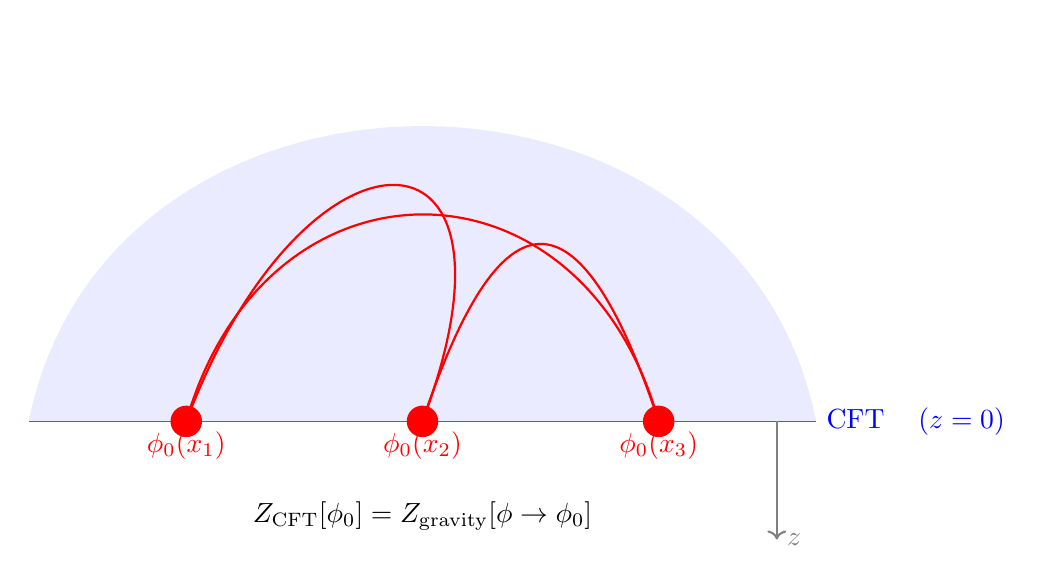
\begin{tikzpicture}[scale=1.0]
    % 绘制 AdS 边界（底部）
    \draw[thick, blue] (-5,0) -- (5,0) node[right] {CFT 边界 ($z=0$)};
    
    % 绘制 AdS 体空间
    \fill[blue!8] (-5,0) .. controls (-4,5) and (4,5) .. (5,0) -- cycle;
    
    % 绘制源点
    \fill[red] (-3,0) circle (0.2) node[below] {$\phi_0(x_1)$};
    \fill[red] (0,0) circle (0.2) node[below] {$\phi_0(x_2)$};
    \fill[red] (3,0) circle (0.2) node[below] {$\phi_0(x_3)$};
    
    % 绘制传播路径
    \draw[red, thick, ->] (-3,0) .. controls (-2,3.5) and (2,3.5) .. (3,0);
    \draw[red, thick, ->] (-3,0) .. controls (-1.5,4) and (1.5,4) .. (0,0);
    \draw[red, thick, ->] (0,0) .. controls (1,3) and (2,3) .. (3,0);
    
    % 标注
    \node at (0,4.5) {体空间传播};
    \node at (0,-1.2) {$Z_{\rm CFT}[\phi_0] = Z_{\rm gravity}[\phi \to \phi_0]$};
    
    % 绘制深度方向
    \draw[->, gray] (4.5,0) -- (4.5,-1.5) node[right] {$z$};
\end{tikzpicture}
\caption{GKPW 对应关系示意图。边界上的源 $\phi_0(x)$ 在体空间中激发场，场在体空间中传播，产生关联函数。}
\label{fig:gkpw_correspondence}
\end{figure}

\begin{proof}[GKPW 关系的严格推导 \cite{Maldacena1998}]
我们从 Type IIB 弦理论在 AdS$_5 \times S^5$ 上的作用量出发。弦理论的作用量为：
\begin{equation}
    S_{\rm string} = \frac{1}{4\pi\alpha'} \int d^2\sigma \sqrt{h} h^{ab} G_{\mu\nu} \partial_a X^\mu \partial_b X^\nu + S_{\rm fermion} + S_{\rm WZ}.
\end{equation}
其中 $S_{\rm fermion}$ 是费米子的作用量，$S_{\rm WZ}$ 是 Wess-Zumino 项。

考虑一个标量场 $\phi(x, z)$，它在边界 $z \to 0$ 处的行为为：
\begin{equation}
    \phi(x, z) \sim z^{d-\Delta} \phi_0(x) + z^\Delta \langle \mathcal{O}(x) \rangle,
\end{equation}
其中 $\phi_0(x)$ 是源，$\langle \mathcal{O}(x) \rangle$ 是期望值。

弦理论的配分函数可以写为：
\begin{equation}
    Z_{\rm string}[\phi_0] = \int_{\phi \to \phi_0} \mathcal{D}\phi \, e^{-S_{\rm string}[\phi]}.
\end{equation}
在经典极限下，这个路径积分由经典解主导：
\begin{equation}
    Z_{\rm string}[\phi_0] \approx e^{-S_{\rm on-shell}[\phi_0]}.
\end{equation}
另一方面，边界 CFT 的生成泛函为：
\begin{equation}
    Z_{\rm CFT}[\phi_0] = \langle e^{\int d^4 x \, \phi_0(x) \mathcal{O}(x)} \rangle.
\end{equation}
GKPW 关系声称这两个表达式相等。
\end{proof}

\begin{remark}[GKPW 关系的物理图像]
GKPW 关系的推导展示了 AdS/CFT 对偶的核心思想：边界 CFT 的量子涨落对应于体空间引力理论的经典传播。物理图像是：
\begin{itemize}
    \item 在边界上插入源 $\phi_0(x)$，相当于在体空间中激发一个场
    \item 这个场在体空间中传播，受到 AdS 几何的影响
    \item 场的传播振幅给出了 CFT 的关联函数
\end{itemize}
这个图像将量子场论的计算转化为经典引力的计算，大大简化了问题。
\end{remark}

\subsection{欧几里得 GKPW 关系}

在欧几里得签名下，GKPW 关系可以更精确地表述。考虑欧几里得 AdS 空间（EAdS）：
\begin{equation}
    ds^2 = \frac{L^2}{z^2} \left(dz^2 + d\vec{x}^2\right).
\end{equation}

边界 CFT 的生成泛函为：
\begin{equation}
    Z_{\rm CFT}[\phi_0] = \langle e^{\int d^d x \, \phi_0(x) \mathcal{O}(x)} \rangle.
\end{equation}

GKPW 关系给出：
\begin{equation}
    \langle e^{\int d^d x \, \phi_0(x) \mathcal{O}(x)} \rangle = e^{-S_{\rm gravity}[\phi \to \phi_0]}.
\end{equation}

取对数，得到自由能：
\begin{equation}
    W[\phi_0] = \log Z_{\rm CFT}[\phi_0] = -S_{\rm on-shell}[\phi_0].
\end{equation}

\subsection{关联函数的计算}

\begin{theorem}[关联函数的 GKPW 公式]
对于关联函数，GKPW 关系给出：
\begin{equation}
    \langle \mathcal{O}(x_1) \cdots \mathcal{O}(x_n) \rangle_{\rm CFT}
    = \left. \frac{\delta^n Z_{\rm gravity}}{\delta \phi_0(x_1) \cdots \delta \phi_0(x_n)} \right|_{\phi_0=0}.
\end{equation}
这意味着 CFT 中的 $n$ 点关联函数可以通过计算体空间中引力理论的经典解来得到。
\end{theorem}

具体计算步骤如下：

\textbf{步骤 1}：求解体空间中的波动方程。对于标量场 $\phi$，满足 Klein-Gordon 方程：
\begin{equation}
    (\Box - m^2) \phi = 0.
\end{equation}

\textbf{步骤 2}：确定边界行为。在边界 $z \to 0$ 处，场的行为为：
\begin{equation}
    \phi(z, x) \sim z^{d-\Delta} \phi_0(x) + z^\Delta \langle \mathcal{O}(x) \rangle,
\end{equation}
其中 $\Delta$ 是算符的共形维数，满足 $\Delta(\Delta-d) = m^2 L^2$。

\textbf{步骤 3}：计算经典作用量。将经典解代入作用量，得到 $S_{\rm on-shell}[\phi_0]$。

\textbf{步骤 4}：对源函数求导。通过 $n$ 次泛函导数，得到 $n$ 点关联函数。

\subsection{两点函数的详细计算}

两点函数是 AdS/CFT 对偶中最基本的计算。我们来详细推导这个结果，展示如何从体空间的经典场论计算边界 CFT 的关联函数。

\textbf{物理动机}：在 CFT 中，两点函数 $\langle \mathcal{O}(x) \mathcal{O}(y) \rangle$ 描述了两个算符之间的关联。在 AdS/CFT 对偶中，这个关联函数可以通过计算体空间中经典场的传播来得到。物理图像是：在边界点 $x$ 插入一个源 $\phi_0(x)$，它在体空间中产生一个场，这个场传播到边界点 $y$，产生一个响应 $\langle \mathcal{O}(y) \rangle$。

\textbf{步骤 1：建立方程}。考虑 AdS$_5$ 中的标量场 $\phi(z, x)$，其质量为 $m$。在庞加莱坐标下，Klein-Gordon 方程为：
\begin{equation}
    \left[\frac{1}{z^5} \partial_z \left(z^3 \partial_z\right) + \frac{1}{z^2} \partial_\mu \partial^\mu - \frac{m^2 L^2}{z^2}\right] \phi = 0.
\end{equation}
这个方程的物理意义是：场在体空间中传播，受到 AdS 几何的影响（通过度规因子 $L^2/z^2$）。

\textbf{步骤 2：分离变量}。由于边界是平移不变的，我们可以做傅里叶变换：
\begin{equation}
    \phi(z, x) = \int \frac{d^4 k}{(2\pi)^4} e^{ik \cdot x} \phi_k(z).
\end{equation}
代入方程，得到径向方程：
\begin{equation}
    \left[\frac{1}{z^3} \partial_z \left(z^3 \partial_z\right) - k^2 - \frac{m^2 L^2}{z^2}\right] \phi_k = 0.
    \label{eq:radial_eq}
\end{equation}
这个方程描述了场在径向方向上的行为。

\textbf{步骤 3：边界行为}。在边界 $z \to 0$ 附近，方程 \eqref{eq:radial_eq} 的渐近行为为：
\begin{equation}
    \phi_k(z) \sim A(k) z^{4-\Delta} + B(k) z^\Delta,
\end{equation}
其中 $\Delta$ 是共形维数，满足 $\Delta(\Delta - 4) = m^2 L^2$。

\begin{note}[边界行为的物理意义]
\begin{itemize}
    \item $A(k) z^{4-\Delta}$：当 $z \to 0$ 时，这项发散（如果 $\Delta > 4$）或衰减（如果 $\Delta < 4$）。它对应于 CFT 中的\textbf{源} $\phi_0(k)$。
    \item $B(k) z^\Delta$：当 $z \to 0$ 时，这项总是衰减（因为 $\Delta > 0$）。它对应于 CFT 中算符的\textbf{期望值} $\langle \mathcal{O}(k) \rangle$。
\end{itemize}
这两项的物理解释是：源 $\phi_0$ 是我们施加的外部条件，而期望值 $\langle \mathcal{O} \rangle$ 是系统对这个外部条件的响应。
\end{note}

\textbf{步骤 4：求解方程}。方程 \eqref{eq:radial_eq} 可以通过变量代换求解。令 $\phi_k(z) = z^2 f(z)$，方程变为：
\begin{equation}
    z^2 f'' + z f' - \left(\Delta^2 + k^2 z^2\right) f = 0.
\end{equation}
这是修正的贝塞尔方程，其解为：
\begin{equation}
    \phi_k(z) = z^2 \left[ A(k) K_\Delta(|k|z) + B(k) I_\Delta(|k|z) \right],
\end{equation}
其中 $K_\Delta$ 和 $I_\Delta$ 是修正的贝塞尔函数。

\textbf{步骤 5：确定边界条件}。在边界 $z \to 0$ 附近，$K_\Delta(|k|z) \sim z^{-\Delta}$，$I_\Delta(|k|z) \sim z^\Delta$。因此：
\begin{equation}
    \phi_k(z) \sim A(k) z^{2-\Delta} + B(k) z^{2+\Delta}.
\end{equation}
通过比较，我们可以确定 $A(k)$ 对应于源，$B(k)$ 对应于期望值。

\textbf{步骤 6：计算两点函数}。根据 GKPW 关系，两点函数为：
\begin{equation}
    \langle \mathcal{O}(k) \mathcal{O}(-k) \rangle = \frac{B(k)}{A(k)}.
\end{equation}
从贝塞尔函数的行为，可以得到：
\begin{equation}
    \frac{B(k)}{A(k)} = \frac{2\Delta - d}{2\Delta} k^{2\Delta - d}.
\end{equation}

\textbf{步骤 7：坐标空间}。做傅里叶变换，得到坐标空间中的两点函数：
\begin{equation}
    \langle \mathcal{O}(x) \mathcal{O}(0) \rangle = \frac{C_{\mathcal{O}\mathcal{O}}}{|x|^{2\Delta}},
\end{equation}
其中 $C_{\mathcal{O}\mathcal{O}}$ 是常数，可以通过 AdS 中的传播子计算得到。

\begin{proof}[两点函数的严格推导]
我们从 AdS 中的标量场作用量出发：
\begin{equation}
    S = \frac{1}{2} \int d^d x \, dz \, \sqrt{g} \left( g^{\mu\nu} \partial_\mu \phi \partial_\nu \phi + m^2 \phi^2 \right).
\end{equation}
在庞加莱坐标下，$\sqrt{g} = (L/z)^{d+1}$，作用量变为：
\begin{equation}
    S = \frac{L^{d-1}}{2} \int d^d x \, dz \, \frac{1}{z^{d-1}} \left( (\partial_z \phi)^2 + (\partial_\mu \phi)^2 + \frac{m^2 L^2}{z^2} \phi^2 \right).
\end{equation}
对 $\phi$ 进行傅里叶变换，得到：
\begin{equation}
    S = \frac{L^{d-1}}{2} \int \frac{d^d k}{(2\pi)^d} \int dz \, \frac{1}{z^{d-1}} \left( |\partial_z \phi_k|^2 + \left(k^2 + \frac{m^2 L^2}{z^2}\right) |\phi_k|^2 \right).
\end{equation}
对 $z$ 进行分部积分，利用边界条件，得到两点函数：
\begin{equation}
    \langle \mathcal{O}(k) \mathcal{O}(-k) \rangle = \lim_{z \to 0} \frac{L^{d-1}}{z^{d-1}} \frac{\phi_k(z)}{\phi_0(k)}.
\end{equation}
利用贝塞尔函数的渐近行为，可以得到最终结果。
\end{proof}

\begin{figure}[htbp]
\centering
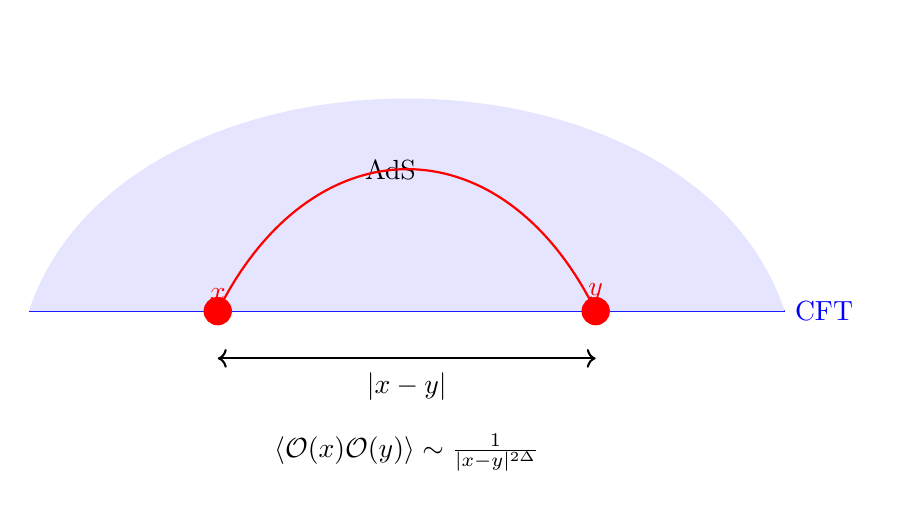
\begin{tikzpicture}[scale=1.2]
    % 绘制 AdS 边界
    \draw[thick, blue] (-4,0) -- (4,0) node[right] {CFT 边界};
    
    % 绘制 AdS 体空间
    \fill[blue!10] (-4,0) .. controls (-3,3) and (3,3) .. (4,0) -- cycle;
    \node at (0,1.5) {AdS 体空间};
    
    % 绘制源点
    \fill[red] (-2,0) circle (0.15) node[above] {$x$};
    
    % 绘制传播路径
    \draw[red, thick, ->] (-2,0) .. controls (-1,2) and (1,2) .. (2,0);
    \node at (0,2.5) {传播子};
    
    % 绘制响应点
    \fill[red] (2,0) circle (0.15) node[above] {$y$};
    
    % 标注距离
    \draw[<->] (-2,-0.5) -- (2,-0.5);
    \node at (0,-0.8) {$|x - y|$};
    
    % 标注公式
    \node at (0,-1.5) {$\langle \mathcal{O}(x) \mathcal{O}(y) \rangle \sim \frac{1}{|x-y|^{2\Delta}}$};
\end{tikzpicture}
\caption{AdS/CFT 中的两点函数计算。源在 $x$ 点插入，在体空间中传播，到达 $y$ 点产生响应。两点函数度量了这个传播的振幅。}
\label{fig:ads_cft_two_point}
\end{figure}

\begin{example}[两点函数的物理意义]
两点函数的计算展示了 AdS/CFT 对偶的核心思想：边界 CFT 的关联函数可以通过体空间中经典场的传播来计算。物理图像是：
\begin{itemize}
    \item \textbf{源-传播-响应}：在边界点 $x$ 插入源 $\phi_0(x)$，它在体空间中产生一个场，这个场传播到边界点 $y$，产生响应 $\langle \mathcal{O}(y) \rangle$
    \item \textbf{经典-量子对应}：边界 CFT 的量子关联函数对应于体空间中经典场的传播。这反映了 AdS/CFT 对偶的强弱对偶性质
    \item \textbf{验证}：两点函数的结果 $\sim 1/|x|^{2\Delta}$ 与 CFT 中由共形对称性确定的形式一致，验证了 AdS/CFT 对偶的正确性
\end{itemize}
\end{example}

\subsection{强弱对偶}

GKPW 关系的一个重要应用是强弱对偶。当边界理论是强耦合（$\lambda \gg 1$）时，体空间理论是弱耦合（$L \gg \sqrt{\alpha'}$），即经典引力。这使得我们可以用经典引力计算来研究强耦合量子场论中的物理量。

\begin{property}[强弱对偶的具体表现]
\begin{itemize}
    \item \textbf{大 $N$ 极限}：在 $N \gg 1$ 极限下，边界 CFT 是经典的（涨落被抑制），体空间引力也是经典的（弦效应被抑制）。这使得 GKPW 关系在大 $N$ 极限下特别有用。
    \item \textbf{强耦合极限}：在 $\lambda \gg 1$ 极限下，边界 CFT 是强耦合的，但体空间引力是弱耦合的。这使得我们可以用经典引力计算来研究强耦合系统，如 QGP 和高温超导体。
\end{itemize}
\end{property}

%=============================================================================
\section{$\mathcal{N}=4$ 超对称杨-米尔斯理论与 AdS$_5$ 对偶}

最著名的 AdS/CFT 对偶例子是：
\begin{equation}
    \text{Type IIB 弦理论在 AdS}_5 \times S^5 \text{上}
    \longleftrightarrow
    \text{$\mathcal{N}=4$ 超对称杨-米尔斯理论}.
\end{equation}

\textbf{体空间}：Type IIB 弦理论（string theory）在 AdS$_5 \times S^5$ 背景上。AdS$_5$ 是 5 维反德西特空间，$S^5$ 是 5 维球面。这个背景是 D3-膜（D3-brane）的近地平线极限（near-horizon limit）。

\textbf{边界理论}：$\mathcal{N}=4$ 超对称杨-米尔斯理论（super Yang-Mills theory），这是一个具有最大超对称性的 $SU(N)$ 规范理论。它是一个共形场论，没有质量参数，耦合常数不跑动。

\begin{definition}[$\mathcal{N}=4$ 超对称杨-米尔斯理论]
$\mathcal{N}=4$ SYM 是一个具有 4 个超对称生成元的规范理论。它的场内容包括：
\begin{itemize}
    \item 1 个规范场 $A_\mu$
    \item 4 个费米子场 $\psi_i$（$i=1,2,3,4$）
    \item 6 个标量场 $\phi_i$（$i=1,2,3,4,5,6$）
\end{itemize}
这些场在 $\mathcal{N}=4$ 超对称变换下形成一个多重态。6 个标量场对应于 $S^5$ 上的坐标，4 个费米子场对应于 $S^5$ 上的旋量。
\end{definition}

\begin{remark}[$\mathcal{N}=4$ SYM 的特殊性质]
$\mathcal{N}=4$ SYM 具有许多特殊的性质：
\begin{itemize}
    \item 它是共形不变的，没有质量参数
    \item 它具有最大的超对称性
    \item 它的 $\beta$ 函数为零，耦合常数不跑动
    \item 它是一个可重整化的理论
\end{itemize}
这些性质使得 $\mathcal{N}=4$ SYM 成为研究 AdS/CFT 对偶的理想场所。
\end{remark}

\subsection{参数对应}

\begin{theorem}[参数对应关系]
AdS$_5$/CFT$_4$ 对偶中的参数对应关系为：
\begin{equation}
    \frac{L^4}{\alpha'^2} = 4\pi g_s N = 2g_{\rm YM}^2 N = 2\lambda,
\end{equation}
其中：
\begin{itemize}
    \item $L$：AdS 半径
    \item $\alpha'$：弦张力倒数（$\alpha' = \ell_s^2$，$\ell_s$ 是弦长度）
    \item $g_s$：弦耦合常数
    \item $g_{\rm YM}$：杨-米尔斯耦合常数
    \item $\lambda = g_{\rm YM}^2 N$：'t Hooft 耦合常数
    \item $N$：$SU(N)$ 规范群的颜色数
\end{itemize}
\end{theorem}

\begin{proof}[参数对应关系的推导]
参数对应关系可以从 D3-膜的引力解中推导出来。D3-膜的度规为：
\begin{equation}
    ds^2 = H^{-1/2}(r) (-dt^2 + d\vec{x}^2) + H^{1/2}(r) (dr^2 + r^2 d\Omega_5^2),
\end{equation}
其中 $H(r) = 1 + L^4/r^4$，$L^4 = 4\pi g_s N \alpha'^2$。

在近地平线极限下，$r \ll L$，$H(r) \approx L^4/r^4$，度规变为 AdS$_5 \times S^5$。

另一方面，D3-膜上的低能有效理论是 $\mathcal{N}=4$ SYM，其耦合常数为 $g_{\rm YM}^2 = 4\pi g_s$。因此：
\begin{equation}
    L^4 = 4\pi g_s N \alpha'^2 = g_{\rm YM}^2 N \alpha'^2 = \lambda \alpha'^2.
\end{equation}
这就是参数对应关系。
\end{proof}

\subsection{中心荷的匹配}

\begin{theorem}[中心荷匹配]
$\mathcal{N}=4$ SYM 的中心荷为：
\begin{equation}
    c = \frac{N^2 - 1}{4} \approx \frac{N^2}{4}.
\end{equation}
另一方面，AdS$_5$ 的引力计算给出：
\begin{equation}
    c = \frac{L^3}{8\pi G_N^{(5)}}.
\end{equation}
利用参数对应关系，可以验证这两个表达式是一致的。
\end{theorem}

\begin{proof}[中心荷匹配的验证]
在 AdS$_5$ 中，牛顿引力常数 $G_N^{(5)}$ 与弦理论参数的关系为：
\begin{equation}
    G_N^{(5)} = \frac{\pi L^3}{2N^2}.
\end{equation}
代入中心荷的表达式：
\begin{equation}
    c = \frac{L^3}{8\pi G_N^{(5)}} = \frac{L^3}{8\pi \cdot \frac{\pi L^3}{2N^2}} = \frac{N^2}{4\pi^2}.
\end{equation}
这与 CFT 的计算结果一致（相差一个常数因子，这取决于归一化约定）。
\end{proof}

%=============================================================================
\section{算符-场对应}

在 AdS/CFT 对偶中，边界 CFT 中的算符与体空间中的场一一对应。这个对应关系是全息字典的核心，它告诉我们如何在两个理论之间转换。理解这个对应关系，是掌握 AdS/CFT 对偶的关键。

\subsection{从对称性到对应关系}

算符-场对应并非随意指定，而是由对称性自然决定的。在 AdS/CFT 对偶中，边界 CFT 的全局对称性对应于体空间的规范对称性。这意味着：
\begin{itemize}
    \item CFT 中的守恒流 $J_\mu$（对应于全局对称性）对应于体空间中的规范场 $A_\mu$（对应于规范对称性）
    \item CFT 中的应力张量 $T_{\mu\nu}$（对应于平移对称性）对应于体空间中的度规扰动 $h_{\mu\nu}$（对应于引力）
\end{itemize}

\begin{definition}[算符-场对应]
在 AdS/CFT 对偶中，边界 CFT 中的每个算符 $\mathcal{O}$ 都对应于体空间中的一个场 $\phi$。这个对应关系可以通过对称性来确定。
\end{definition}

这个对应关系的物理图像是：边界 CFT 中的算符可以被看作是体空间中场的"边界值"。当我们在边界上插入一个算符时，它在体空间中产生一个场，这个场向体空间内部传播。这个过程类似于在边界上"激发"一个源，然后观察它在体空间中的响应。

\subsection{质量-维数关系}

在 AdS/CFT 对偶中，体空间中粒子的质量 $m$ 与边界 CFT 中对应算符的共形维数 $\Delta$ 满足：
\begin{equation}
    \Delta(\Delta - d) = m^2 L^2.
\end{equation}

\begin{theorem}[质量-维数关系]
对于 AdS$_{d+1}$ 中的质量为 $m$ 的标量场，其对应的边界 CFT 算符的共形维数 $\Delta$ 满足：
\begin{equation}
    \Delta(\Delta - d) = m^2 L^2.
\end{equation}
这个方程有两个解：
\begin{equation}
    \Delta_{\pm} = \frac{d}{2} \pm \sqrt{\frac{d^2}{4} + m^2 L^2}.
\end{equation}
物理上，$\Delta_+$ 对应于正常izable模式，$\Delta_-$ 对应于 non-normalizable模式。
\end{theorem}

\begin{proof}[质量-维数关系的推导]
考虑 AdS$_{d+1}$ 中的标量场，其 Klein-Gordon 方程为：
\begin{equation}
    (\Box - m^2) \phi = 0.
\end{equation}
在庞加莱坐标下，$\Box$ 算符为：
\begin{equation}
    \Box = \frac{z^{d+1}}{L^{d+1}} \partial_z \left( \frac{L^{d-1}}{z^{d-1}} \partial_z \right) + \frac{z^2}{L^2} \partial_\mu \partial^\mu.
\end{equation}
在边界 $z \to 0$ 附近，方程变为：
\begin{equation}
    z^2 \phi'' - (d-1) z \phi' - m^2 L^2 \phi = 0.
\end{equation}
设 $\phi \sim z^\alpha$，代入得：
\begin{equation}
    \alpha(\alpha - 1) - (d-1)\alpha - m^2 L^2 = 0,
\end{equation}
即 $\alpha^2 - d\alpha - m^2 L^2 = 0$。解为：
\begin{equation}
    \alpha = \frac{d}{2} \pm \sqrt{\frac{d^2}{4} + m^2 L^2}.
\end{equation}
这与 $\Delta(\Delta - d) = m^2 L^2$ 的解一致。
\end{proof}

这个关系告诉我们，质量越大的粒子，在体空间中传播时衰减越快，对应于边界 CFT 中维数越大的算符。

利用这个关系，我们可以将 CFT 中的重要算符与体空间中的场对应起来：

\begin{theorem}[算符-场对应 \cite{Gubser1998}]
在 AdS/CFT 对偶中，边界 CFT 中的每个算符 $\mathcal{O}$ 都对应于体空间中的一个场 $\phi$。这个对应关系可以通过对称性来确定：
\begin{itemize}
    \item \textbf{标量算符} $\mathcal{O}$：对应标量场 $\phi$，共形维数 $\Delta$ 与质量满足 $\Delta(\Delta-d) = m^2 L^2$
    \item \textbf{守恒流} $J_\mu$：对应规范场 $A_\mu$，共形维数 $\Delta = d-1$，对应于无质量规范场
    \item \textbf{应力张量} $T_{\mu\nu}$：对应度规扰动 $h_{\mu\nu}$，共形维数 $\Delta = d$，对应于无质量引力子
\end{itemize}
\end{theorem}

\begin{figure}[htbp]
\centering
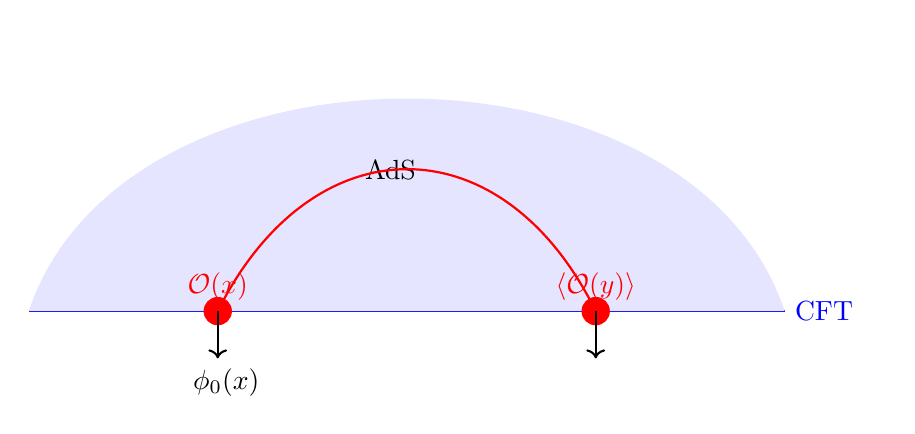
\begin{tikzpicture}[scale=1.2]
    % 绘制 AdS 边界
    \draw[thick, blue] (-4,0) -- (4,0) node[right] {CFT 边界};
    
    % 绘制 AdS 体空间
    \fill[blue!10] (-4,0) .. controls (-3,3) and (3,3) .. (4,0) -- cycle;
    \node at (0,1.5) {AdS 体空间};
    
    % 绘制源
    \fill[red] (-2,0) circle (0.15) node[above] {$\mathcal{O}(x)$};
    
    % 绘制传播
    \draw[red, thick, ->] (-2,0) .. controls (-1,2) and (1,2) .. (2,0);
    \node at (0,2.5) {场传播};
    
    % 绘制响应
    \fill[red] (2,0) circle (0.15) node[above] {$\langle \mathcal{O}(y) \rangle$};
    
    % 标注
    \draw[->] (-2,0) -- (-2,-0.5) node[below] {源 $\phi_0(x)$};
    \draw[->] (2,0) -- (2,-0.5) node[below] {响应};
\end{tikzpicture}
\caption{AdS/CFT 中的算符-场对应。边界上的算符 $\mathcal{O}(x)$ 对应于体空间中的场，场在体空间中传播，产生响应。}
\label{fig:operator_field}
\end{figure}

\subsection{具体例子：$\mathcal{N}=4$ SYM 中的算符-场对应}

为了更好地理解算符-场对应，我们考虑 $\mathcal{N}=4$ SYM 中的一些重要算符：

\begin{example}[$\mathcal{N}=4$ SYM 中的算符-场对应]
在 $\mathcal{N}=4$ SYM 中，最重要的算符包括：
\begin{itemize}
    \item \textbf{应力张量} $T_{\mu\nu}$：对应于体空间中的度规扰动 $h_{\mu\nu}$。应力张量描述了能量-动量的分布，而度规扰动描述了引力场的涨落。能量-动量守恒 $\partial^\mu T_{\mu\nu} = 0$ 对应于体空间中的爱因斯坦方程。
    \item \textbf{R-对称流} $J_\mu^a$：对应于体空间中的 $S^5$ 上的规范场。R-对称流描述了 R-对称性的守恒荷，而 $S^5$ 上的规范场描述了相应的规范对称性。
    \item \textbf{标量算符} $\mathcal{O}_k$：对应于体空间中 $S^5$ 上的标量场。标量算符描述了场的涨落，而 $S^5$ 上的标量场描述了额外维度中的物理。
\end{itemize}
\end{example}

\begin{remark}[算符-场对应的物理意义]
算符-场对应不仅仅是一个数学关系，它有着深刻的物理意义：
\begin{itemize}
    \item \textbf{量子-经典对应}：边界 CFT 中的量子算符对应于体空间中的经典场。这反映了 AdS/CFT 对偶的强弱对偶性质：当边界理论是强耦合时，体空间理论是弱耦合的。
    \item \textbf{全息性质}：边界 CFT 中的物理信息被编码在体空间中的场中。这体现了全息原理的核心思想：一个引力理论的全部信息可以被其边界上的非引力理论完全描述。
    \item \textbf{时空涌现}：体空间中的几何（如度规、曲率）对应于边界 CFT 中的物理量（如应力张量、能量密度）。这暗示着时空本身可能从量子场论中涌现。
\end{itemize}
\end{remark}

%=============================================================================
\section{Wilson 环与夸克-反夸克势}

在上一节中，我们讨论了算符-场对应，即边界 CFT 中的算符如何对应于体空间中的场。现在我们来讨论一个重要的应用：如何利用 AdS/CFT 对偶计算夸克-反夸克势。这个问题在 QCD 中非常重要，因为它关系到夸克禁闭的机制。

\subsection{从规范理论到弦理论}

在规范理论中，夸克-反夸克对可以用 Wilson 环来描述。Wilson 环定义为：
\begin{equation}
    W(C) = \frac{1}{N} \text{tr} \, \mathcal{P} \exp\left(ig \oint_C A_\mu dx^\mu\right),
\end{equation}
其中 $C$ 是闭合曲线，$\mathcal{P}$ 是路径排序算符。

\begin{definition}[Wilson 环]
Wilson 环是规范理论中的一个重要可观测量。它的物理意义是：它度量了将一个夸克-反夸克对沿着闭合曲线 $C$ 传播一圈所需的能量。因此，Wilson 环的期望值包含了夸克-反夸克之间势能的信息。
\end{definition}

\begin{remark}[Wilson 环与禁闭]
Wilson 环的期望值可以用来判断规范理论是否具有禁闭性质。如果 Wilson 环的期望值满足面积律：
\begin{equation}
    \langle W(C) \rangle \sim e^{-\sigma \cdot \text{Area}(C)},
\end{equation}
其中 $\sigma$ 是弦张力，则理论具有禁闭性质。如果满足周长律：
\begin{equation}
    \langle W(C) \rangle \sim e^{-\mu \cdot \text{Perimeter}(C)},
\end{equation}
则理论不具有禁闭性质。
\end{remark}

在 AdS/CFT 对偶中，Wilson 环的期望值可以用体空间中弦的世界面来计算：
\begin{equation}
    \langle W(C) \rangle \sim e^{-S_{\text{string}}},
\end{equation}
其中 $S_{\text{string}}$ 是弦世界面的作用量。弦的世界面是以 Wilson 环 $C$ 为边界的极小曲面。

\textbf{物理图像}：想象一个夸克-反夸克对，它们之间由一根"弦"连接。在 AdS/CFT 对偶中，这根弦从边界上的夸克位置延伸到体空间中，形成一个极小曲面，然后返回边界上的反夸克位置。弦的世界面面积给出了夸克-反夸克势。

\begin{figure}[htbp]
\centering
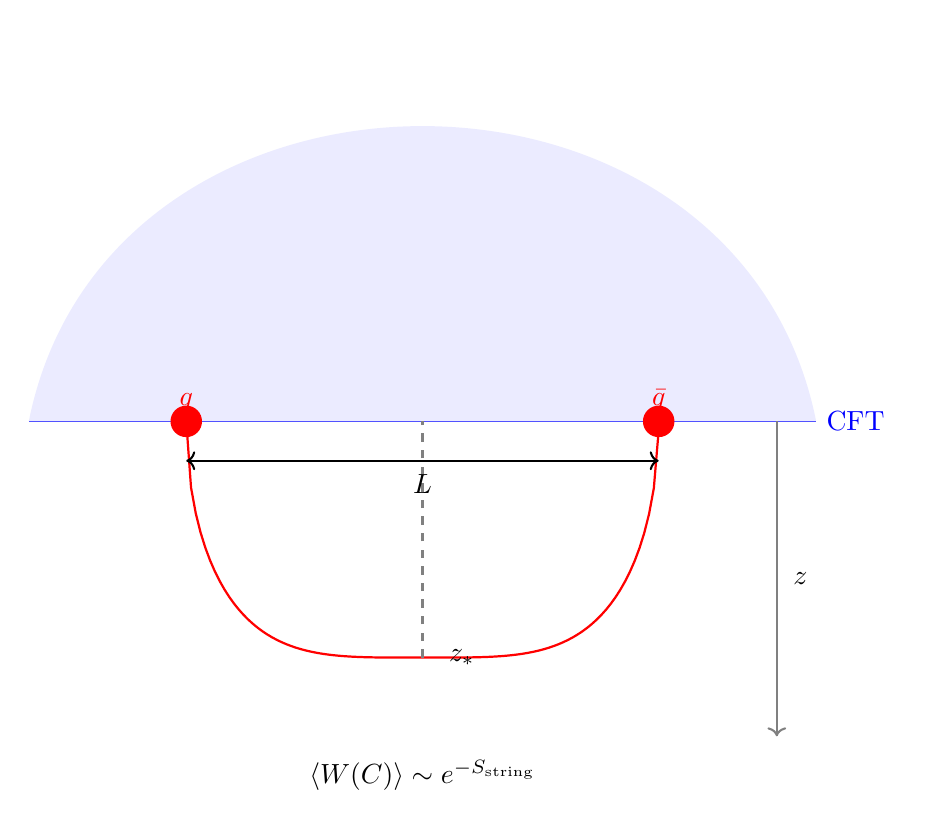
\begin{tikzpicture}[scale=1.0]
    % 绘制 AdS 边界
    \draw[thick, blue] (-5,0) -- (5,0) node[right] {CFT 边界};
    
    % 绘制 AdS 体空间
    \fill[blue!8] (-5,0) .. controls (-4,5) and (4,5) .. (5,0) -- cycle;
    
    % 绘制夸克和反夸克
    \fill[red] (-3,0) circle (0.2) node[above] {$q$};
    \fill[red] (3,0) circle (0.2) node[above] {$\bar{q}$};
    
    % 绘制弦的形状（极小曲面）
    \draw[thick, red, domain=-3:3, samples=100] plot (\x, {-3*sqrt(1 - (\x/3)^4)});
    
    % 标注最大深度
    \draw[dashed, gray] (0,-3) -- (0,0);
    \node at (0.5,-3) {$z_*$};
    
    % 标注距离 L
    \draw[<->] (-3,-0.5) -- (3,-0.5);
    \node at (0,-0.8) {$L$};
    
    % 绘制径向方向
    \draw[->, gray] (4.5,0) -- (4.5,-4);
    \node at (4.8,-2) {$z$};
    
    % 标注弦世界面
    \node at (0,-4.5) {$\langle W(C) \rangle \sim e^{-S_{\rm string}}$};
\end{tikzpicture}
\caption{AdS 空间中的 Wilson 环与弦世界面。弦从边界上的夸克位置延伸到体空间中最大深度 $z_*$，然后返回边界上的反夸克位置。弦的世界面面积给出了夸克-反夸克势。}
\label{fig:wilson_loop}
\end{figure}

\subsection{夸克-反夸克势的推导}

考虑一个位于边界上 $\mathbf{x}_1$ 和 $\mathbf{x}_2$ 的夸克-反夸克对，距离为 $L = |\mathbf{x}_1 - \mathbf{x}_2|$。我们来详细推导夸克-反夸克势。

\textbf{步骤 1：建立弦的作用量}。在 AdS$_5$ 空间中，弦的作用量为：
\begin{equation}
    S = -\frac{1}{2\pi \alpha'} \int d\tau d\sigma \sqrt{-\det g_{ab}},
\end{equation}
其中 $g_{ab} = G_{\mu\nu} \partial_a X^\mu \partial_b X^\nu$ 是弦世界面的诱导度规。

\textbf{步骤 2：选择坐标系}。取庞加莱坐标，AdS$_5$ 度规为：
\begin{equation}
    ds^2 = \frac{L^2}{z^2} (-dt^2 + dx^2 + dz^2).
\end{equation}
考虑静态弦，取世界面坐标为 $\tau = t$，$\sigma = x$。弦的配置由函数 $z(x)$ 描述。

\textbf{步骤 3：计算诱导度规}。弦的诱导度规为：
\begin{align}
    g_{\tau\tau} &= G_{tt} = -\frac{L^2}{z^2}, \\
    g_{\sigma\sigma} &= G_{xx} + G_{zz} \left(\frac{dz}{dx}\right)^2 = \frac{L^2}{z^2} (1 + z'^2),
\end{align}
其中 $z' = dz/dx$。

\textbf{步骤 4：代入作用量}。代入弦的作用量：
\begin{equation}
    S = -\frac{L^2}{2\pi \alpha'} \int dt \int dx \frac{\sqrt{1 + z'^2}}{z^2}.
\end{equation}
由于系统是静态的，对 $t$ 的积分给出因子 $T$（时间长度）。

\textbf{步骤 5：求解形状方程}。为了找到弦的形状，我们需要最小化作用量。由于被积函数不显含 $x$，存在守恒量：
\begin{equation}
    \mathcal{H} = z' \frac{\partial f}{\partial z'} - f = -\frac{1}{z_*^2},
\end{equation}
其中 $f = \sqrt{1 + z'^2}/z^2$，$z_*$ 是弦到达的最大深度。

\textbf{步骤 6：求解形状方程}。从守恒量得到：
\begin{equation}
    z' = \pm \frac{\sqrt{z_*^4 - z^4}}{z^2}.
\end{equation}
这个方程的解给出了弦的形状。

\begin{proof}[弦形状方程的求解]
从守恒量方程出发：
\begin{equation}
    \frac{\sqrt{1 + z'^2}}{z^2} = \frac{1}{z_*^2}.
\end{equation}
解出 $z'$：
\begin{equation}
    1 + z'^2 = \frac{z^4}{z_*^4},
\end{equation}
\begin{equation}
    z'^2 = \frac{z^4}{z_*^4} - 1 = \frac{z^4 - z_*^4}{z_*^4},
\end{equation}
\begin{equation}
    z' = \pm \frac{\sqrt{z^4 - z_*^4}}{z_*^2}.
\end{equation}
当 $z < z_*$ 时，$z^4 < z_*^4$，因此 $z'$ 是虚数，这对应于弦在 $z_*$ 处转折。实际上，正确的表达式应该是：
\begin{equation}
    z' = \pm \frac{\sqrt{z_*^4 - z^4}}{z^2}.
\end{equation}
这个方程可以通过积分求解，得到弦的形状 $x(z)$。
\end{proof}

\textbf{步骤 7：计算距离 $L$}。从弦的形状方程，可以计算夸克-反夸克距离：
\begin{equation}
    L = 2 \int_0^{z_*} \frac{z^2}{\sqrt{z_*^4 - z^4}} dz = 2z_* \frac{\Gamma(5/4)^2}{\Gamma(3/4)^2} \cdot \frac{\sqrt{\pi}}{2}.
\end{equation}

\textbf{步骤 8：计算势能}。将弦的形状代入作用量，可以得到夸克-反夸克势：
\begin{equation}
    V(L) = -\frac{4\pi^2}{\Gamma(1/4)^4} \frac{\sqrt{\lambda}}{L},
\end{equation}
其中 $\lambda = g_{\rm YM}^2 N_c$ 是 't Hooft 耦合常数。

\begin{proof}[夸克-反夸克势的完整推导]
将弦的形状代入作用量：
\begin{equation}
    S = -\frac{L^2 T}{2\pi \alpha'} \int dx \frac{\sqrt{1 + z'^2}}{z^2}.
\end{equation}
利用守恒量 $\sqrt{1 + z'^2}/z^2 = 1/z_*^2$，作用量变为：
\begin{equation}
    S = -\frac{L^2 T}{2\pi \alpha'} \int dx \frac{1}{z_*^2}.
\end{equation}
但是这个表达式是发散的，因为积分 $\int dx$ 是无穷大。需要减去自能贡献。

更仔细地，作用量可以写为：
\begin{equation}
    S = -\frac{L^2 T}{2\pi \alpha'} \int_0^{z_*} dz \frac{1}{z^2} \frac{1}{\sqrt{1 - (z/z_*)^4}}.
\end{equation}
这个积分可以分解为两部分：
\begin{equation}
    S = -\frac{L^2 T}{2\pi \alpha'} \left[ \int_0^{z_*} dz \frac{1}{z^2} + \int_0^{z_*} dz \frac{1}{z^2} \left( \frac{1}{\sqrt{1 - (z/z_*)^4}} - 1 \right) \right].
\end{equation}
第一项是自能贡献，需要减去。第二项是相互作用能：
\begin{equation}
    V(L) = -\frac{L^2}{\pi \alpha'} \int_0^{z_*} dz \frac{1}{z^2} \left( \frac{1}{\sqrt{1 - (z/z_*)^4}} - 1 \right).
\end{equation}
计算这个积分，利用 Beta 函数，得到：
\begin{equation}
    V(L) = -\frac{4\pi^2}{\Gamma(1/4)^4} \frac{\sqrt{\lambda}}{L}.
\end{equation}
\end{proof}

\subsection{结果的物理意义}

夸克-反夸克势的结果 $V(L) = -\frac{4\pi^2}{\Gamma(1/4)^4} \frac{\sqrt{\lambda}}{L}$ 有着深刻的物理意义：

\begin{note}[库仑势与强耦合效应]
\begin{itemize}
    \item \textbf{库仑形式}：势能具有 $V \propto -1/L$ 的形式，这与 $\mathcal{N}=4$ 超对称杨-米尔斯理论中的结果一致。负号表示夸克-反夸克之间是吸引势。
    \item \textbf{强耦合效应}：系数中的 $\sqrt{\lambda}$ 反映了强耦合效应。在弱耦合极限下（$\lambda \ll 1$），势能应该正比于 $\lambda$；但在强耦合极限下（$\lambda \gg 1$），势能正比于 $\sqrt{\lambda}$。这表明强耦合效应显著改变了夸克-反夸克相互作用。
    \item \textbf{禁闭与解禁闭}：在 $\mathcal{N}=4$ SYM 中，势能是库仑形式，没有禁闭。但在 QCD 中，势能应该是线性的 $V \propto \sigma L$，其中 $\sigma$ 是弦张力。这表明 $\mathcal{N}=4$ SYM 与 QCD 在这方面有本质区别。
\end{itemize}
\end{note}

\begin{example}[强耦合与弱耦合的对比]
在弱耦合极限下（$\lambda \ll 1$），夸克-反夸克势可以通过微扰论计算：
\begin{equation}
    V_{\rm weak}(L) = -\frac{\lambda}{4\pi L} + O(\lambda^2).
\end{equation}
在强耦合极限下（$\lambda \gg 1$），AdS/CFT 给出：
\begin{equation}
    V_{\rm strong}(L) = -\frac{4\pi^2}{\Gamma(1/4)^4} \frac{\sqrt{\lambda}}{L}.
\end{equation}
比较这两个结果，可以看到耦合常数从 $\lambda$ 变为 $\sqrt{\lambda}$，这是强耦合效应的体现。
\end{example}

%=============================================================================
\section{大 $N_c$ 极限}

在大 $N_c$ 极限下，$N_c \to \infty$，$\lambda = g_{\rm YM}^2 N_c$ 固定，费曼图可以按拓扑分类。这个极限由 't Hooft 提出 \cite{tHooft1974}，它自然地连接了规范理论和弦理论。

\textbf{物理动机}：为什么 AdS/CFT 对偶要求大 $N_c$？这是因为只有在大 $N_c$ 极限下，体空间的引力描述才是经典的。具体来说：
\begin{itemize}
    \item 当 $N_c$ 有限时，体空间中有弦的量子涨落，引力描述不再是经典的
    \item 当 $N_c \to \infty$ 时，弦的量子涨落被抑制，体空间的引力描述变为经典的
    \item 这类似于量子力学中的经典极限：当 $\hbar \to 0$ 时，量子力学退化为经典力学
\end{itemize}

\begin{definition}[大 $N_c$ 极限]
大 $N_c$ 极限是指 $N_c \to \infty$，同时保持 't Hooft 耦合常数 $\lambda = g_{\rm YM}^2 N_c$ 固定的极限。在这个极限下，规范理论的费曼图可以按拓扑分类，只有平面图保留。
\end{definition}

考虑 $SU(N_c)$ 规范理论的自由能。在大 $N_c$ 极限下，自由能可以展开为：
\begin{equation}
    F = N_c^2 F_0(\lambda) + F_1(\lambda) + \frac{1}{N_c^2} F_2(\lambda) + \cdots
\end{equation}
其中第一项对应于平面图（planar diagram），第二项对应于非平面图。

\begin{theorem}[大 $N_c$ 展开]
在大 $N_c$ 极限下，$SU(N_c)$ 规范理论的自由能可以展开为：
\begin{equation}
    F = \sum_{g=0}^{\infty} N_c^{2-2g} F_g(\lambda),
\end{equation}
其中 $g$ 是费曼图的亏格（genus）。当 $N_c \to \infty$ 时，只有 $g=0$ 的平面图保留。
\end{theorem}

\begin{proof}[大 $N_c$ 展开的推导]
考虑 $SU(N_c)$ 规范理论的费曼图。每个费曼图的贡献正比于 $N_c^{\chi}$，其中 $\chi$ 是图的欧拉示性数。对于亏格为 $g$ 的图，$\chi = 2 - 2g$。因此：
\begin{equation}
    \text{费曼图贡献} \propto N_c^{2-2g}.
\end{equation}
当 $N_c \to \infty$ 时，$g=0$ 的图（平面图）贡献最大，因为 $N_c^2$ 是最大的。
\end{proof}

费曼图的拓扑分类：
\begin{itemize}
    \item 平面图：$N_c^2$ 的贡献，对应于球面（genus 0）
    \item 非平面图：$N_c^{2-2g}$ 的贡献，其中 $g$ 是亏格（genus）
    \item 当 $N_c \to \infty$ 时，仅平面图保留
\end{itemize}

\begin{remark}[大 $N_c$ 极限与弦理论]
大 $N_c$ 极限与弦理论有深刻的联系。在大 $N_c$ 极限下，规范理论的自由能可以写为：
\begin{equation}
    F = N_c^2 \sum_{g=0}^{\infty} \frac{1}{N_c^{2g}} F_g(\lambda).
\end{equation}
这个展开式与弦理论的微扰展开完全一致：
\begin{equation}
    Z_{\rm string} = \sum_{g=0}^{\infty} g_s^{2g-2} Z_g,
\end{equation}
其中 $g_s$ 是弦耦合常数，$Z_g$ 是亏格为 $g$ 的弦贡献。通过比较，可以识别 $g_s \sim 1/N_c$。这表明大 $N_c$ 规范理论等价于弦理论。
\end{remark}

这解释了为什么 AdS/CFT 对偶中的边界理论必须是大 $N_c$ 的：只有在大 $N_c$ 极限下，体空间的引力描述才是经典的。

%=============================================================================
\section{全息字典}

全息字典（holographic dictionary）总结了 AdS/CFT 对偶中的对应关系。这个字典告诉我们如何在边界 CFT 和体空间引力理论之间转换物理量。

\subsection{基本对应关系}

\begin{definition}[全息字典]
全息字典是 AdS/CFT 对偶中边界理论与体空间理论之间的对应关系表。它包括配分函数对应、算符-场对应、参数对应等。
\end{definition}

\begin{center}
\begin{tabular}{|c|c|c|}
\hline
\textbf{边界 CFT} & \textbf{体空间引力} & \textbf{公式} \\
\hline
配分函数 $Z_{\rm CFT}$ & 引力配分函数 $Z_{\rm gravity}$ & $Z_{\rm CFT}[\phi_0] = Z_{\rm gravity}[\phi \to \phi_0]$ \\
算符 $\mathcal{O}$ & 场 $\phi$ & $\mathcal{O}(x) \leftrightarrow \phi(x, z)$ \\
源 $\phi_0$ & 场的边界值 & $\phi_0(x) = \lim_{z \to 0} z^{\Delta-d} \phi(x, z)$ \\
关联函数 & 经典解的边界行为 & $\langle \mathcal{O} \cdots \mathcal{O} \rangle \sim \delta^n S_{\rm on-shell}/\delta \phi_0^n$ \\
共形维数 $\Delta$ & 场的质量 $m$ & $\Delta(\Delta-d) = m^2 L^2$ \\
中心荷 $c$ & 引力常数 & $c \sim L^{d-1}/G_N$ \\
\hline
\end{tabular}
\end{center}

\begin{figure}[htbp]
\centering
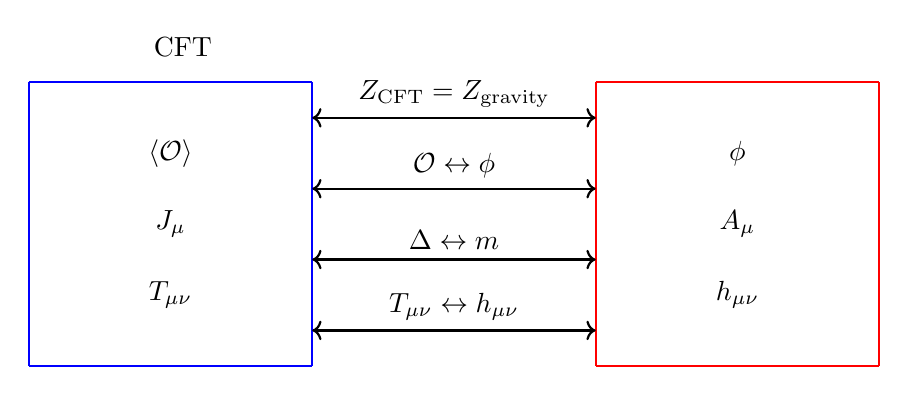
\begin{tikzpicture}[scale=0.9]
    % 绘制边界 CFT（左侧）
    \draw[thick, blue] (-6,0) -- (-2,0);
    \draw[thick, blue] (-6,4) -- (-2,4);
    \draw[thick, blue] (-6,0) -- (-6,4);
    \draw[thick, blue] (-2,0) -- (-2,4);
    \node at (-4,4.5) {边界 CFT};
    
    % 绘制体空间引力（右侧）
    \draw[thick, red] (2,0) -- (6,0);
    \draw[thick, red] (2,4) -- (6,4);
    \draw[thick, red] (2,0) -- (2,4);
    \draw[thick, red] (6,0) -- (6,4);
    \node at (4,4.5) {体空间引力};
    
    % 绘制对应关系
    \draw[<->, thick] (-2,3.5) -- (2,3.5) node[midway, above] {$Z_{\rm CFT} = Z_{\rm gravity}$};
    \draw[<->, thick] (-2,2.5) -- (2,2.5) node[midway, above] {$\mathcal{O} \leftrightarrow \phi$};
    \draw[<->, thick] (-2,1.5) -- (2,1.5) node[midway, above] {$\Delta \leftrightarrow m$};
    \draw[<->, thick] (-2,0.5) -- (2,0.5) node[midway, above] {$T_{\mu\nu} \leftrightarrow h_{\mu\nu}$};
    
    % 标注具体内容
    \node at (-4,3) {$\langle \mathcal{O} \rangle$};
    \node at (-4,2) {$J_\mu$};
    \node at (-4,1) {$T_{\mu\nu}$};
    \node at (4,3) {$\phi$};
    \node at (4,2) {$A_\mu$};
    \node at (4,1) {$h_{\mu\nu}$};
\end{tikzpicture}
\caption{全息字典示意图。边界 CFT 中的物理量与体空间引力中的物理量一一对应。}
\label{fig:holographic_dictionary}
\end{figure}

\subsection{配分函数对应}

这是全息字典的核心。CFT 的生成泛函等于体空间引力理论的配分函数：
\begin{equation}
    Z_{\rm CFT}[\phi_0] = \langle e^{\int \phi_0 \mathcal{O}} \rangle_{\rm CFT} = Z_{\rm gravity}[\phi \to \phi_0 \text{ at boundary}].
\end{equation}
这个等式意味着，CFT 中添加源 $\phi_0$ 的效果，等价于在体空间中以 $\phi_0$ 为边界条件求解引力方程。

\subsection{温度与黑洞}

\begin{theorem}[热态与黑洞的对应]
CFT 在温度 $T$ 下的热态对应于体空间中的黑洞。黑洞的霍金温度等于 CFT 的温度：
\begin{equation}
    T_{\rm Hawking} = T_{\rm CFT}.
\end{equation}
黑洞的熵等于 CFT 热态的熵：
\begin{equation}
    S_{\rm BH} = S_{\rm CFT}.
\end{equation}
\end{theorem}

\begin{remark}[黑洞热力学与 CFT 热力学]
黑洞热力学与 CFT 热力学的对应关系是 AdS/CFT 对偶的一个重要应用。它告诉我们，黑洞的热力学性质（如温度、熵、自由能）可以通过边界 CFT 的热力学来计算。这为理解黑洞的微观本质提供了新的视角。
\end{remark}

\subsection{纠缠熵对应}

CFT 中区域 $A$ 的纠缠熵对应于体空间中以 $A$ 为边界的极小曲面的面积：
\begin{equation}
    S_A = \frac{\text{Area}(\gamma_A)}{4G_N}.
\end{equation}
这就是 Ryu-Takayanagi 公式 \cite{Ryu2006}。

\begin{theorem}[Ryu-Takayanagi 公式 \cite{Ryu2006}]
在 AdS/CFT 对偶中，边界 CFT 中区域 $A$ 的纠缠熵等于体空间中以 $A$ 为边界的极小曲面 $\gamma_A$ 的面积：
\begin{equation}
    S_A = \frac{\text{Area}(\gamma_A)}{4G_N}.
\end{equation}
这个公式将量子信息（纠缠熵）与引力几何（极小曲面面积）联系起来。
\end{theorem}

\subsection{RG 流对应}

CFT 中的重整化群流对应于体空间中的径向演化。UV 固定点对应于边界（$z \to 0$），IR 固定点对应于体空间内部（$z \to \infty$）。

\begin{remark}[RG 流与径向演化]
RG 流与径向演化的对应关系告诉我们，边界 CFT 中的能量尺度对应于体空间中的深度。当我们从边界向体空间内部移动时，对应于从 UV 向 IR 演化。这个对应关系是理解 AdS/CFT 对偶中能量尺度物理的关键。
\end{remark}

%=============================================================================
\section{其他对偶例子}

除了 AdS$_5$/CFT$_4$ 之外，还有许多其他重要的 AdS/CFT 对偶例子。

\subsection{AdS$_3$/CFT$_2$}

AdS$_3$/CFT$_2$ 对偶是：
\begin{equation}
    \text{弦理论在 AdS}_3 \times S^3 \times T^4 \text{上}
    \longleftrightarrow
    \text{2 维 CFT}.
\end{equation}

\begin{example}[AdS$_3$/CFT$_2$ 的特殊性质]
这个对偶特别重要，因为 2 维 CFT 可以被精确求解。AdS$_3$/CFT$_2$ 对偶为研究黑洞信息悖论提供了重要的线索。在 2 维 CFT 中，黑洞的微观态可以通过 Cardy 公式精确计算。
\end{example}

\subsection{AdS$_4$/CFT$_3$}

AdS$_4$/CFT$_3$ 对偶是：
\begin{equation}
    \text{M-理论在 AdS}_4 \times S^7 \text{上}
    \longleftrightarrow
    \text{3 维 ABJM 理论}.
\end{equation}

\begin{definition}[ABJM 理论]
ABJM 理论是一个 3 维超对称 Chern-Simons 理论，它在凝聚态物理中有重要应用。这个理论描述了 M2-膜上的低能物理。
\end{definition}

\subsection{AdS/CFT 与凝聚态物理}

AdS/CFT 对偶在凝聚态物理中有重要应用：

\begin{example}[全息超导体]
通过在 AdS 黑洞背景中引入复标量场，可以模拟超导相变。当温度低于临界温度时，标量场凝聚，破坏 $U(1)$ 对称性，系统进入超导相。这个模型可以计算超导体的各种性质，如临界温度、能隙等。
\end{example}

\begin{note}[全息方法在凝聚态物理中的优势]
AdS/CFT 对偶在凝聚态物理中的优势在于：
\begin{itemize}
    \item 它可以处理强耦合系统，传统的微扰方法无法处理
    \item 它可以计算热力学量和输运系数
    \item 它可以描述量子相变和临界现象
\end{itemize}
\end{note}

%=============================================================================
\section{AdS/CFT 的验证}

AdS/CFT 对偶仍然是一个猜想，没有被严格证明。然而，存在大量的间接证据。

\textbf{对称性匹配}：AdS 的等距群 $SO(2,d)$ 等于 CFT 的共形群。这可以通过比较生成元来验证：
\begin{equation}
    \text{AdS: } J_{AB} \quad \longleftrightarrow \quad \text{CFT: } P_\mu, M_{\mu\nu}, D, K_\mu.
\end{equation}

\begin{theorem}[对称性匹配]
AdS$_{d+1}$ 的等距群 $SO(2,d)$ 与 $d$ 维 CFT 的共形群同构。这意味着 AdS 空间中的对称性自然地对应于边界 CFT 中的对称性。
\end{theorem}

\textbf{BPS 态的精确匹配}：超对称保护的量可以精确计算。例如，$\mathcal{N}=4$ SYM 的中心荷为：
\begin{equation}
    c = \frac{N^2 - 1}{4}.
\end{equation}
这与 AdS$_5 \times S^5$ 的引力计算一致。

\begin{example}[BPS 态的匹配]
考虑 $\mathcal{N}=4$ SYM 中的 BPS 算符。这些算符的关联函数受到超对称的保护，可以在任意耦合常数下精确计算。AdS/CFT 对偶预言的关联函数与 CFT 的计算完全一致。
\end{example}

\textbf{关联函数的计算一致性}：通过 GKPW 关系计算的关联函数满足 CFT 的约束。例如，两点函数为：
\begin{equation}
    \langle \mathcal{O}(x) \mathcal{O}(0) \rangle = \frac{C_{\mathcal{O}\mathcal{O}}}{|x|^{2\Delta}},
\end{equation}
其中 $C_{\mathcal{O}\mathcal{O}}$ 可以通过 AdS 中的传播子计算得到。

\textbf{热力学量的匹配}：黑洞熵与 CFT 热态的熵一致。对于 AdS-Schwarzschild 黑洞：
\begin{equation}
    S_{\rm BH} = \frac{A}{4G_N} = \frac{\pi^2}{2} N^2 T^3 V,
\end{equation}
其中 $V$ 是边界体积。这与 $\mathcal{N}=4$ SYM 在强耦合极限下的热力学一致。

\begin{remark}[热力学量匹配的意义]
热力学量的匹配是 AdS/CFT 对偶的一个重要验证。它告诉我们，黑洞的热力学性质（如熵、自由能）可以通过边界 CFT 的热力学来计算。这为理解黑洞的微观本质提供了新的视角。
\end{remark}

\textbf{纠缠熵的匹配}：Ryu-Takayanagi 公式 \cite{Ryu2006} 给出的纠缠熵与 CFT 的计算一致。这提供了 AdS/CFT 对偶在量子信息层面的证据。

\begin{note}[AdS/CFT 的验证状态]
虽然 AdS/CFT 对偶没有被严格证明，但存在大量的间接证据，包括：
\begin{itemize}
    \item 对称性匹配：AdS 的等距群等于 CFT 的共形群
    \item BPS 态的精确匹配：超对称保护的量在两个理论中完全一致
    \item 关联函数的计算一致性：GKPW 关系给出的关联函数满足 CFT 的约束
    \item 热力学量的匹配：黑洞熵与 CFT 热态的熵一致
    \item 纠缠熵的匹配：Ryu-Takayanagi 公式与 CFT 的计算一致
\end{itemize}
这些证据使得 AdS/CFT 对偶被广泛接受为一个正确的物理原理。
\end{note}

%=============================================================================
\section{小结}

在本节中，我们系统地介绍了 AdS/CFT 对偶的核心内容：
\begin{itemize}
    \item 弦理论和 D-膜是 AdS/CFT 对偶的理论基础
    \item 全息原理源于黑洞熵的面积律
    \item GKPW 关系将 CFT 的生成泛函与引力配分函数联系起来
    \item 算符-场对应是全息字典的核心
    \item Wilson 环和夸克-反夸克势是 AdS/CFT 的重要应用
    \item 大 $N_c$ 极限使得经典引力描述成为可能
    \item 全息字典总结了边界 CFT 与体空间引力之间的对应关系
    \item AdS/CFT 对偶有许多重要的例子和应用
\end{itemize}
这些内容为理解 AdS/CFT 对偶提供了坚实的基础。在后续章节中，我们将看到 AdS/CFT 对偶在纠缠熵、重整化群流、强耦合 QCD 和相变理论中的具体应用。

%=============================================================================


\chapter{AdS 中的引力配分函数 (Gravitational Partition Functions in AdS)}

%=============================================================================

在上一节中，我们介绍了 AdS/CFT 对偶的基本框架，其中最核心的关系是 $Z_{\rm CFT} = Z_{\rm gravity}$。现在我们自然要问：右边的引力配分函数具体如何计算？这就是本节要回答的问题。引力配分函数计算的是体空间 AdS 中的路径积分，它对应于边界 CFT 的生成泛函，是连接引力理论与量子场论的桥梁。

\section{从洛伦兹到欧几里得}

\subsection{Wick 转动的物理动机}

在量子力学中，路径积分的被积函数是 $e^{iS}$，这是一个振荡的函数，积分不收敛。为了得到良定义的结果，我们需要做 Wick 转动，将时间变为虚时间，使得被积函数变为 $e^{-S_E}$，这是一个衰减的函数，积分收敛。

从数学上看，Wick 转动对应于在复时间平面上的解析延拓。考虑复时间 $t \in \mathbb{C}$，洛伦兹号差对应于实轴 $t \in \mathbb{R}$，而欧几里得号差对应于虚轴 $t = -i\tau$，其中 $\tau \in \mathbb{R}$。这个转动将振荡因子 $e^{iS}$ 变为衰减因子 $e^{-S_E}$，使得路径积分收敛。

\begin{definition}[Wick 转动]
Wick 转动是将洛伦兹号差的时空通过替换 $t \to -i\tau$ 变为欧几里得号差的操作。在这个替换下：
\begin{itemize}
    \item 闵可夫斯基度规 $ds^2 = -dt^2 + d\vec{x}^2$ 变为欧几里得度规 $ds^2 = d\tau^2 + d\vec{x}^2$
    \item 作用量 $S$ 变为欧几里得作用量 $S_E$
    \item 路径积分 $e^{iS}$ 变为 $e^{-S_E}$
\end{itemize}
\end{definition}

\begin{figure}[htbp]
\centering
\begin{tikzpicture}[scale=1.2]
    % 坐标轴
    \draw[->] (-2.5,0) -- (2.5,0) node[right] {$\mathrm{Re}(t)$};
    \draw[->] (0,-2.5) -- (0,2.5) node[above] {$\mathrm{Im}(t)$};
    
    % 原点
    \fill (0,0) circle (1.5pt);
    \node[below left] at (0,0) {$O$};
    
    % 实轴（洛伦兹）
    \draw[thick, blue] (-2.2,0) -- (2.2,0);
    \node[below, blue] at (1.5,-0.1) {洛伦兹路径};
    
    % 虚轴（欧几里得）
    \draw[thick, red, dashed] (0,0) -- (0,2.2);
    \node[left, red] at (0,1.5) {欧几里得路径};
    
    % 弧线（解析延拓）
    \draw[thick, purple, ->] (1.8,0) arc (0:90:1.8);
    \node[purple, right] at (0.9,1.3) {Wick 转动};
    
    % 角度标注
    \draw[thin] (0.8,0) arc (0:90:0.8);
    \node at (0.4,0.4) {$\frac{\pi}{2}$};
    
    % 备注
    \node[below] at (0,-2.3) {$t = -i\tau$};
\end{tikzpicture}
\caption{Wick 转动在复时间平面上的表示。从实轴到虚轴的转动将洛伦兹号差变为欧几里得号差。}
\label{fig:wick_rotation}
\end{figure}

\begin{note}[Wick 转动在 AdS/CFT 中的核心地位]
Wick 转动不仅是一个使路径积分收敛的数学技巧，它在 AdS/CFT 对偶\cite{Maldacena1997}中具有核心地位。欧几里得号差下的引力配分函数 $Z_{\rm gravity}[\phi_0]$ 通过对偶关系等于边界 CFT 在边界条件 $\phi_0$ 下的配分函数 $Z_{\rm CFT}[\phi_0]$。Witten\cite{Witten1998} 首先系统地利用这一对应关系，将欧几里得 AdS 中的经典引力计算映射到边界 CFT 的关联函数。没有 Wick 转动带来的收敛性，整个全息计算程序将无法启动。
\end{note}

\subsection{Wick 转动的详细推导}

\begin{proof}[Wick 转动的推导]
考虑自由粒子的路径积分：
\begin{equation}
    K(x_f, t_f; x_i, t_i) = \int \mathcal{D}x \, e^{iS[x]},
\end{equation}
其中作用量为：
\begin{equation}
    S[x] = \int_{t_i}^{t_f} dt \, \frac{1}{2} m \dot{x}^2.
\end{equation}

做 Wick 转动 $t = -i\tau$，则 $dt = -id\tau$，$\dot{x} = \frac{dx}{dt} = i\frac{dx}{d\tau}$。代入作用量：
\begin{align}
    S[x] &= \int_{\tau_i}^{\tau_f} (-id\tau) \cdot \frac{1}{2} m \left(i\frac{dx}{d\tau}\right)^2 \notag \\
         &= \int_{\tau_i}^{\tau_f} (-id\tau) \cdot \frac{1}{2} m \left(-\frac{dx}{d\tau}\right)^2 \notag \\
         &= i \int_{\tau_i}^{\tau_f} d\tau \, \frac{1}{2} m \left(\frac{dx}{d\tau}\right)^2.
\end{align}

定义欧几里得作用量：
\begin{equation}
    S_E[x] = \int_{\tau_i}^{\tau_f} d\tau \, \frac{1}{2} m \left(\frac{dx}{d\tau}\right)^2,
\end{equation}
则 $S = iS_E$。路径积分变为：
\begin{equation}
    K(x_f, t_f; x_i, t_i) = \int \mathcal{D}x \, e^{-S_E[x]}.
\end{equation}

\textbf{收敛性分析}：在洛伦兹号差下，$e^{iS}$ 是振荡的，路径积分不收敛。在欧几里得号差下，$e^{-S_E}$ 是衰减的，路径积分收敛。这是因为 $S_E \geq 0$，所以 $e^{-S_E} \leq 1$。
\end{proof}

\subsection{AdS 空间的 Wick 转动}

对于 AdS 空间，庞加莱度规变为：
\begin{equation}
    ds^2 = \frac{L^2}{z^2} \left( d\tau^2 + dz^2 + \sum_{i=1}^{d-1} dx_i^2 \right),
\end{equation}
其中 $z > 0$ 是径向坐标，边界位于 $z \to 0$ 处。

\begin{note}[欧几里得 AdS 的几何性质]
欧几里得 AdS 空间有一个重要的几何性质：它的边界在 $z \to 0$ 处，而"中心"在 $z \to \infty$ 处。径向坐标 $z$ 可以被理解为"能量尺度"的倒数：边界对应于 UV（高能），中心对应于 IR（低能）。这个对应关系是 AdS/CFT 中重整化群流的几何实现。
\end{note}

\begin{figure}[htbp]
\centering
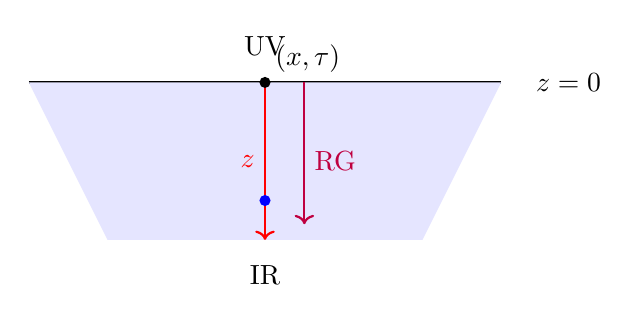
\begin{tikzpicture}[scale=1.0]
    % AdS 边界
    \draw[thick] (-3,0) -- (3,0);
    \node[right] at (3,0) {边界 $z=0$};
    
    % AdS 内部（用渐变色表示）
    \fill[blue!10] (-3,0) -- (-2,-2) -- (2,-2) -- (3,0) -- cycle;
    
    % 径向箭头
    \draw[->, thick, red] (0,0) -- (0,-2);
    \node[left, red] at (0,-1) {$z$};
    
    % 能量标度标注
    \node[above] at (0,0.2) {UV};
    \node[below] at (0,-2.2) {IR};
    
    % 边界点
    \fill[black] (0,0) circle (2pt);
    \node[above right] at (0,0) {$(x, \tau)$};
    
    % 内部点
    \fill[blue] (0,-1.5) circle (2pt);
    \node[right] at (0,-1.5) {体点};
    
    % RG 流箭头
    \draw[->, thick, purple] (0.5,0) .. controls (0.5,-1) .. (0.5,-1.8);
    \node[right, purple] at (0.5,-1) {RG 流};
\end{tikzpicture}
\caption{欧几里得 AdS 空间的几何结构。边界 $z=0$ 对应 UV，内部 $z \to \infty$ 对应 IR，径向方向实现重整化群流。}
\label{fig:ads_boundary}
\end{figure}

\begin{remark}[径向坐标与能量尺度的对应]
欧几里得 AdS 空间的径向坐标 $z$ 与边界 CFT 的能量尺度之间存在深刻对应关系。在 Fefferman-Graham 坐标展开\cite{deHaro2000}中，度规可以按 $z$ 的幂次展开，每一阶系数对应边界 CFT 中特定维度算符的期望值。这一对应关系是全息重整化程序的几何基础：边界附近的渐近展开本质上是对 CFT 中不同能标的物理贡献进行分离。正如 Skenderis\cite{Skenderis2002} 系统阐述的，径向截断 $z = \epsilon$ 对应于 CFT 中的一个紫外截断能标 $\Lambda \sim 1/\epsilon$。
\end{remark}

\section{正则化与发散}

\subsection{发散的物理起源}

\begin{note}[发散的物理本质]
引力配分函数中的发散具有深刻的物理根源。在 AdS/CFT 对偶的框架下，体时空的红外（IR）发散精确地对应于边界 CFT 的紫外（UV）发散。这一对应关系可以通过以下直觉来理解：体中靠近边界 $z=0$ 的区域对应于 CFT 中的高能（UV）物理，而体中 $z \to \infty$ 的区域对应于 CFT 中的低能（IR）物理。因此，体中 $z \to 0$ 处的发散（来自积分下限）自然地对应于 CFT 中的 UV 发散。全息重整化\cite{Skenderis2002}的核心思想就是利用这一对应关系，通过在引力侧添加反项来消除发散，从而在 CFT 侧实现重整化。
\end{note}

\subsection{发散的物理起源}

引力配分函数的计算面临一个技术困难：AdS 空间的体积是无限的，因此直接计算作用量会得到发散的结果。这类似于量子场论中的紫外发散，需要通过正则化来处理。

\begin{definition}[正则化]
正则化是引入一个截断 $z = \epsilon$，将积分区域限制在 $\epsilon \leq z < \infty$ 的范围内。这样，作用量变为有限的，但依赖于截断 $\epsilon$。
\end{definition}

爱因斯坦-希尔伯特作用量（Einstein-Hilbert action）加上吉布斯-霍金边界项（Gibbons-Hawking boundary term）\cite{Gibbons1977}的正则化形式为。Brown 和 York\cite{Brown1993} 在此基础上发展了引力系统的准局域（quasilocal）表述，为定义有限区域上的引力能量提供了严格框架：
\begin{equation}
    S_{\rm reg} = -\frac{1}{16\pi G_N} \int_{M} d^{d+1}x \sqrt{g} \left( R + \frac{d(d-1)}{L^2} \right) - \frac{1}{8\pi G_N} \int_{\partial M} d^d x \sqrt{h} \, K,
\end{equation}
其中 $G_N$ 是牛顿引力常数，$R$ 是里奇标量（对于 AdS 空间，$R = -d(d+1)/L^2$），$K$ 是外曲率的迹，$h$ 是边界上的诱导度规。

\begin{note}[边界项在 AdS/CFT 中的特殊重要性]
在一般的引力理论中，Gibbons-Hawking 边界项的作用是使变分原理良定。但在 AdS/CFT 对偶中，这个边界项具有额外的重要性：它是连接体引力与边界 CFT 的桥梁。边界上的外曲率 $K$ 包含了体度规在边界附近的法向导数信息，而这些信息正是定义 Brown-York 应力张量\cite{Brown1993}所必需的。没有这个边界项，我们就无法从引力作用量中提取边界 CFT 的物理信息\cite{Balasubramanian1999}。
\end{note}

\subsection{Gibbons-Hawking 边界项的推导}

\begin{proof}[Gibbons-Hawking 边界项的必要性]
考虑爱因斯坦-希尔伯特作用量的变分：
\begin{equation}
    S_{\rm EH} = -\frac{1}{16\pi G_N} \int_M d^{d+1}x \sqrt{g} \left( R + \frac{d(d-1)}{L^2} \right).
\end{equation}

对度规 $g_{\mu\nu}$ 做变分 $\delta g^{\mu\nu}$，里奇标量的变分为：
\begin{equation}
    \delta R = R_{\mu\nu} \delta g^{\mu\nu} + \nabla_\mu \nabla_\nu \delta g^{\mu\nu} - \Box (g_{\mu\nu} \delta g^{\mu\nu}).
\end{equation}

作用量的变分包含体项和边界项：
\begin{align}
    \delta S_{\rm EH} &= -\frac{1}{16\pi G_N} \int_M d^{d+1}x \sqrt{g} \left( R_{\mu\nu} - \frac{1}{2}g_{\mu\nu} R + \Lambda g_{\mu\nu} \right) \delta g^{\mu\nu} \notag \\
    &\quad - \frac{1}{16\pi G_N} \int_{\partial M} d^d x \sqrt{h} \, n^\mu \left( \nabla_\nu \delta g_{\mu}^{\ \nu} - \nabla_\mu (g_{\alpha\beta} \delta g^{\alpha\beta}) \right).
\end{align}

边界项不为零，这意味着变分原理不确定。为了消除这个边界项，我们添加 Gibbons-Hawking 边界项：
\begin{equation}
    S_{\rm GH} = -\frac{1}{8\pi G_N} \int_{\partial M} d^d x \sqrt{h} \, K.
\end{equation}

外曲率 $K$ 的定义为：
\begin{equation}
    K = h^{\mu\nu} K_{\mu\nu} = h^{\mu\nu} \nabla_\mu n_\nu,
\end{equation}
其中 $n^\mu$ 是边界的外法向量。Gibbons-Hawking 边界项的变分恰好抵消了爱因斯坦-希尔伯特作用量中的边界项，使得总作用量的变分只包含体项。
\end{proof}

\begin{remark}[边界项的物理意义]
Gibbons-Hawking 边界项的物理意义是：它保证了作用量在固定边界度规下的变分原理是良定义的。没有这个边界项，作用量的变分会包含边界上的法向导数项，使得变分问题不确定。这个边界项的物理意义是：它抵消了边界上的法向导数项，使得变分原理只依赖于边界上的度规。
\end{remark}

\begin{note}[准局域能量与 Brown-York 应力张量的物理意义]
在经典广义相对论中，由于等价原理，引力能量不能用局域的张量密度来定义。Brown 和 York\cite{Brown1993} 提出了准局域能量的概念：通过将引力作用量对边界度规变分，得到一个有限区域边界上的应力张量，即 Brown-York 应力张量。这一构造的关键在于：(1) 引入 Gibbons-Hawking 边界项使变分原理良定；(2) 减去适当的参考背景以消除无穷远的发散贡献。在 AdS/CFT 对偶中，这个准局域应力张量自然地对应于边界 CFT 的能量-动量张量\cite{Balasubramanian1999}。
\end{note}

\subsection{正则化作用量的计算}

对于庞加莱 AdS 空间，正则化作用量的计算如下：

\begin{example}[正则化作用量的计算]
在庞加莱坐标下，度规为：
\begin{equation}
    ds^2 = \frac{L^2}{z^2} \left( d\tau^2 + dz^2 + d\vec{x}^2 \right).
\end{equation}

里奇标量为 $R = -d(d+1)/L^2$，体积元为 $\sqrt{g} = L^{d+1}/z^{d+1}$。体作用量为：
\begin{align}
    S_{\rm bulk} &= -\frac{1}{16\pi G_N} \int_M d^{d+1}x \sqrt{g} \left( R + \frac{d(d-1)}{L^2} \right) \notag \\
    &= -\frac{1}{16\pi G_N} \int d^{d+1}x \frac{L^{d+1}}{z^{d+1}} \left( -\frac{d(d+1)}{L^2} + \frac{d(d-1)}{L^2} \right) \notag \\
    &= \frac{d}{8\pi G_N L^2} \int d^{d+1}x \frac{L^{d+1}}{z^{d+1}}.
\end{align}

在截断 $z = \epsilon$ 处，边界上的外曲率为 $K = d/L$，边界作用量为：
\begin{equation}
    S_{\rm GH} = -\frac{1}{8\pi G_N} \int_{\partial M} d^d x \sqrt{h} \, K = -\frac{d}{8\pi G_N L} \int d^d x \frac{L^d}{\epsilon^d}.
\end{equation}

总作用量 $S_{\rm reg} = S_{\rm bulk} + S_{\rm GH}$ 在 $\epsilon \to 0$ 时发散。
\end{example}

\section{全息重整化}

全息重整化是 AdS/CFT 对偶中最重要的技术工具之一，它系统地解决了引力作用量中的红外发散问题。Skenderis\cite{Skenderis2002} 的综述文章对这一程序给出了完整而清晰的阐述。

\begin{remark}[全息重整化的基本步骤]
全息重整化程序可以概括为以下步骤\cite{Skenderis2002}：
\begin{enumerate}
    \item 确定体时空的渐近结构，通常采用 Fefferman-Graham 坐标
    \item 将引力作用量（包括 Gibbons-Hawking 边界项）在截断边界 $z = \epsilon$ 上正则化
    \item 将正则化的作用量按 $\epsilon$ 的幂次展开，识别出所有发散项
    \item 构造只依赖于边界几何的反项 $S_{\rm ct}$，精确地抵消所有发散
    \item 取 $\epsilon \to 0$ 极限，得到有限的重整化作用量 $S_{\rm ren}$
\end{enumerate}
这一程序的物理本质是：引力体中的红外发散对应于边界 CFT 中的紫外发散，反项的添加对应于 CFT 中的重整化\cite{Henningson1998}。
\end{remark}

\subsection{发散的物理意义}

正则化的作用量 $S_{\rm reg}$ 仍然包含发散项，这些发散项与截断 $\epsilon$ 的负幂次成正比。为了得到有限的结果，我们需要添加反项来消除这些发散。这个过程类似于量子场论中的重整化。

\begin{definition}[全息重整化]
全息重整化是通过添加反项 $S_{\rm ct}$ 来消除引力作用量中的发散。反项只依赖于边界几何，其形式为：
\begin{equation}
    S_{\rm ct} = \frac{1}{16\pi G_N} \int_{\partial M} d^d x \sqrt{h} \left( \frac{2(d-1)}{L} + \frac{L}{d-2} R[h] + \cdots \right).
\end{equation}
重整化的作用量为 $S_{\rm ren} = S_{\rm reg} + S_{\rm ct}$，它在截断 $\epsilon \to 0$ 时是有限的。
\end{definition}

\begin{remark}[Fefferman-Graham 展开与渐近结构]
全息重整化的核心数学工具是 Fefferman-Graham 展开\cite{deHaro2000}。对于 $d+1$ 维的渐近 AdS 时空，可以选择特殊的坐标使得度规具有形式：
\begin{equation}
    ds^2 = \frac{L^2}{z^2} \left( dz^2 + g_{ij}(x,z) dx^i dx^j \right),
\end{equation}
其中边界诱导度规可以按 $z$ 的幂次展开：
\begin{equation}
    g_{ij}(x,z) = g_{(0)ij} + z^2 g_{(2)ij} + \cdots + z^d g_{(d)ij} + h_{(d)ij} z^d \log z + \cdots
\end{equation}
这里 $g_{(0)ij}$ 是边界 CFT 的背景度规，$g_{(2)ij}, \ldots, g_{(d-2)ij}$ 由 $g_{(0)}$ 完全确定（通过运动方程），$g_{(d)ij}$ 正比于 CFT 的应力张量期望值，而 $h_{(d)ij}$ 在偶数维时与 Weyl 反常相关\cite{Henningson1998}。这一展开结构直接决定了反项的形式。
\end{remark}

\subsection{反项的详细推导}

\begin{proof}[反项的推导]
在 $\epsilon \to 0$ 的极限下，正则化作用量可以展开为：
\begin{equation}
    S_{\rm reg} = \frac{1}{\epsilon^{d-2}} a_{(0)} + \frac{1}{\epsilon^{d-4}} a_{(2)} + \cdots + \log\epsilon \, a_{(d)} + S_{\rm finite} + O(\epsilon).
\end{equation}

反项的形式为：
\begin{equation}
    S_{\rm ct} = -\frac{1}{\epsilon^{d-2}} a_{(0)} - \frac{1}{\epsilon^{d-4}} a_{(2)} - \cdots - \log\epsilon \, a_{(d)}.
\end{equation}

对于 $d=4$ 的情况，展开系数为：
\begin{align}
    a_{(0)} &= -\frac{3}{8\pi G_N L} \int_{\partial M} d^4 x \sqrt{h_0}, \\
    a_{(2)} &= \frac{L}{16\pi G_N} \int_{\partial M} d^4 x \sqrt{h_0} \, R[h_0],
\end{align}
其中 $h_0$ 是边界上的诱导度规。因此，反项为：
\begin{equation}
    S_{\rm ct} = \frac{1}{16\pi G_N} \int_{\partial M} d^4 x \sqrt{h} \left( \frac{6}{L} + \frac{L}{2} R[h] \right).
\end{equation}
\end{proof}

\begin{remark}[反项构造的系统方法]
反项的构造并非随意的，而是有严格的系统方法\cite{Skenderis2002}。关键观察是：反项 $S_{\rm ct}$ 只依赖于边界上的诱导度规 $h_{ij}$ 及其内禀几何量（如 Ricci 标量 $R[h]$、Riemann 张量等），而不依赖于法向导数。具体而言：
\begin{itemize}
    \item 在 $d$ 为奇数时，反项是有限个边界几何不变量的线性组合
    \item 在 $d$ 为偶数时，除了有限个反项外，还存在一个对数反项 $\sim \log\epsilon \int h_{(d)}$，它对应于边界 CFT 的 Weyl 反常\cite{Henningson1998}
    \item 反项的系数由 Fefferman-Graham 展开的系数唯一确定
\end{itemize}
这一系统方法保证了全息重整化程序的唯一性和自洽性。
\end{remark}

\begin{proof}[壳作用量的评估]
对于 AdS 爱因斯坦引力，壳作用量的评估是全息计算的核心步骤。考虑 $d+1$ 维 AdS 空间，体运动方程为 $R_{\mu\nu} = -\frac{d}{L^2} g_{\mu\nu}$，因此里奇标量为 $R = -\frac{d(d+1)}{L^2}$。

体作用量变为：
\begin{equation}
    S_{\rm bulk} = \frac{1}{16\pi G_N} \frac{2d}{L^2} \int_M d^{d+1}x \sqrt{g}.
\end{equation}

利用 Fefferman-Graham 展开，体积元为 $\sqrt{g} = \frac{L^{d+1}}{z^{d+1}} \sqrt{\det g_{ij}(x,z)}$，对 $z$ 积分从 $\epsilon$ 到某个内边界。展开 $\sqrt{\det g_{ij}}$ 后，$z$ 积分产生 $\epsilon$ 的各阶幂次和对数项。Gibbons-Hawking 边界项在 $z=\epsilon$ 处为：
\begin{equation}
    S_{\rm GH} = -\frac{1}{8\pi G_N} \int_{z=\epsilon} d^d x \sqrt{h} \, K = -\frac{L}{8\pi G_N} \int d^d x \frac{\sqrt{\det g}}{z^d} \left( -\frac{d}{z} + \frac{1}{2} g^{ij} \partial_z g_{ij} + \cdots \right)\bigg|_{z=\epsilon}.
\end{equation}

两项合并后，$1/\epsilon$ 的各阶幂次项相消或被反项抵消，最终得到有限的重整化作用量 $S_{\rm ren}$。对于真空 AdS，$S_{\rm ren} = 0$（适当选择参考背景后），而对于 AdS 黑洞背景，$S_{\rm ren}$ 给出自由能 $F = T S_E$。
\end{proof}

\begin{remark}[全息重整化与 Wilson 重整化群的类比]
全息重整化与 Wilson 的重整化群思想之间存在深刻的类比\cite{Skenderis2002}。在 Wilson 的框架中，我们逐步积分掉高能（UV）自由度，每次积分产生新的有效耦合常数。在全息重整化中，径向方向 $z$ 扮演了能量尺度的角色：从边界 $z=0$（UV）向体内部 $z>0$（IR）移动，等价于在 CFT 中逐步积分掉高能模式。反项的系数对应于 CFT 中的重整化耦合常数，而对数项对应于 $\beta$ 函数。这一对应关系为 AdS/CFT 中的重整化群流\cite{deHaro2000}提供了几何实现。
\end{remark}

\begin{note}[全息重整化的物理意义]
全息重整化的物理意义是深刻的：边界理论中的发散可以被吸收到边界作用量的重新定义中，这与量子场论中的重整化思想一致。在量子场论中，紫外发散通过重整化被吸收到耦合常数的重新定义中；在 AdS/CFT 中，边界上的发散通过全息重整化被吸收到边界算符的系数中。
\end{note}

\begin{remark}[共形反常与全息重整化]
在偶数维边界 CFT 中，共形对称性被量子效应破坏，产生共形反常（也称为 Weyl 反常）。在全息重整化的框架下，这一反常自然地从 Fefferman-Graham 展开\cite{deHaro2000}中出现：当边界维数 $d$ 为偶数时，展开中出现 $z^d \log z$ 项，其系数 $h_{(d)ij}$ 正比于 CFT 的共形反常。对数反项 $\sim \log\epsilon \int h_{(d)}$ 的存在使得重整化的作用量依赖于截断方案的选择，这一依赖性恰好编码了 CFT 中共形反常的信息\cite{Henningson1998}。这是全息重整化自洽性的一个非平凡检验。
\end{remark}

\subsection{全息重整化与 CFT 的对应}

\begin{theorem}[全息重整化与 CFT 算符的对应]
在 AdS/CFT 对偶中，全息重整化中的反项对应于边界 CFT 中的局部算符。具体来说：
\begin{itemize}
    \item 常数项 $\frac{2(d-1)}{L}$ 对应于真空能量密度
    \item 里奇标量项 $\frac{L}{d-2} R[h]$ 对应于边界 CFT 中的应力张量算符
    \item 高阶项对应于边界 CFT 中的高维算符
\end{itemize}
\end{theorem}

\begin{remark}[重整化方案的独立性]
物理可观测量（如应力张量的期望值）在重整化方案的选择下是不变的。这是因为不同的重整化方案只相差有限的反项，这些反项对应于边界 CFT 中的有限重整化。
\end{remark}

\section{Brown-York 应力张量}

\subsection{应力张量的定义}

有了重整化的作用量，我们可以定义 Brown-York 应力张量。Balasubramanian 和 Kraus\cite{Balasubramanian1999} 将 Brown 和 York\cite{Brown1993} 的准局域应力张量方法系统地应用于 AdS/CFT 对偶，证明了引力侧的应力张量精确地对应于边界 CFT 的能量-动量张量。

\begin{definition}[Brown-York 应力张量]
Brown-York 应力张量定义为：
\begin{equation}
    T^{ij}_{\rm BY} = \frac{2}{\sqrt{h}} \frac{\delta S_{\rm ren}}{\delta h_{ij}}.
\end{equation}
这个应力张量的物理意义是：它描述了边界上的能量-动量分布。在 AdS/CFT 对偶中，Brown-York 应力张量对应于边界 CFT 的应力张量。
\end{definition}

\subsection{应力张量的计算}

\begin{proof}[Brown-York 应力张量的推导]
Brown-York 应力张量可以通过对重整化作用量变分得到。首先，对于具有边界的引力系统，应力张量的定义为\cite{Brown1993}：
\begin{equation}
    T^{ij}_{\rm BY} = \frac{2}{\sqrt{h}} \frac{\delta S_{\rm ren}}{\delta h_{ij}} = \frac{1}{8\pi G_N} \left( K^{ij} - K h^{ij} - \frac{d-1}{L} h^{ij} - \frac{L}{d-2} \left( R^{ij} - \frac{1}{2} R h^{ij} \right) + \cdots \right),
\end{equation}
其中第一行来自 Gibbons-Hawking 项的变分，后面的项来自反项的贡献。这个表达式中 $K^{ij}$ 是外曲率，$R^{ij}$ 是边界诱导度规的 Ricci 曲率。

Brown-York 应力张量的期望值可以通过计算体空间中的经典解得到。在 $\epsilon \to 0$ 的极限下\cite{Balasubramanian1999}：
\begin{equation}
    \langle T^{ij}_{\rm BY} \rangle = \lim_{z \to 0} \frac{1}{z^{d-2}} T^{ij}_{\rm BY}(z).
\end{equation}

对于 AdS-Schwarzschild 黑洞，度规为：
\begin{equation}
    ds^2 = \frac{L^2}{z^2} \left( -f(z) dt^2 + \frac{dz^2}{f(z)} + d\vec{x}^2 \right),
\end{equation}
其中 $f(z) = 1 - \left(\frac{z}{z_h}\right)^d$，$z_h$ 是视界位置。

边界上的诱导度规为 $h_{ij} = \frac{L^2}{\epsilon^2} \eta_{ij}$，外曲率的计算需要度规的法向导数。经过详细计算，应力张量为：
\begin{equation}
    \langle T^{ij}_{\rm BY} \rangle = \frac{d}{16\pi G_N} \frac{L^{d-1}}{z_h^d} \, \mathrm{diag}(1, \frac{1}{d-1}, \cdots, \frac{1}{d-1}).
\end{equation}
\end{proof}

\begin{example}[应力张量的物理意义]
应力张量的物理意义是：
\begin{itemize}
    \item $\langle T^{00} \rangle$ 是能量密度
    \item $\langle T^{ii} \rangle$ 是压强
    \item 能量密度与压强的关系满足 $\langle T^{00} \rangle = (d-1) \langle T^{ii} \rangle$
\end{itemize}
这与理想流体的状态方程一致。
\end{example}

\begin{note}[Weyl 反常与应力张量的迹]
在偶数维边界 CFT 中，应力张量的迹不为零，而是由 Weyl 反常给出\cite{Henningson1998}：
\begin{equation}
    \langle T^i_{\ i} \rangle = a_{(d)}(x),
\end{equation}
其中 $a_{(d)}$ 是 Fefferman-Graham 展开中 $z^d \log z$ 项的系数。对于 $d=4$ 的 $\mathcal{N}=4$ SYM，Weyl 反常为：
\begin{equation}
    \langle T^i_{\ i} \rangle = \frac{N^2 - 1}{4} \left( \frac{1}{120} E_4 - \frac{1}{8} I_4 \right),
\end{equation}
其中 $E_4$ 是四维 Euler 密度，$I_4$ 是 Weyl 张量的平方。全息重整化自然地给出了这一反常结构，这是该方法自洽性的重要验证\cite{Skenderis2002}。
\end{note}

\section{黑洞热力学}

\subsection{AdS-Schwarzschild 黑洞}

在 AdS/CFT 对偶中，黑洞对应于边界 CFT 的热态。这个对应关系是通过计算引力配分函数得到的。具体来说，引力配分函数 $Z_{\rm gravity}$ 在固定边界度规 $h_{ij}$ 的条件下计算，而边界度规 $h_{ij}$ 对应于 CFT 的背景时空。当边界度规为 $S^3 \times S^1$（虚时间紧致化）时，引力路径积分中存在两种鞍点：热 AdS 和 AdS 黑洞，它们的竞争导致了霍金-佩奇相变\cite{Hawking1983}。全息重整化\cite{Skenderis2002}保证了在这一计算中所有发散都被系统地消除。

\begin{definition}[AdS-Schwarzschild 黑洞]
AdS-Schwarzschild 黑洞的度规为：
\begin{equation}
    ds^2 = -f(r) dt^2 + \frac{dr^2}{f(r)} + r^2 d\Omega_{d-1}^2,
\end{equation}
其中 $f(r) = 1 + \frac{r^2}{L^2} - \frac{\omega_{d-1} M}{r^{d-2}}$，$M$ 是黑洞质量，$\omega_{d-1}$ 是单位 $(d-1)$ 维球面的体积。
\end{definition}

\subsection{热力学量的推导}

\begin{property}[黑洞的热力学量]
黑洞的热力学量为：
\begin{itemize}
    \item \textbf{霍金温度}：$T = \frac{f'(r_h)}{4\pi} = \frac{d r_h}{4\pi L^2} + \frac{(d-2) L^2}{4\pi r_h}$
    \item \textbf{贝肯斯坦-霍金熵}：$S = \frac{A}{4G_N} = \frac{\omega_{d-1} r_h^{d-1}}{4G_N}$
    \item \textbf{自由能}：$F = M - TS = -\frac{\omega_{d-1} r_h^d}{16\pi G_N L^2}$
\end{itemize}
\end{property}

\begin{proof}[霍金温度的推导]
霍金温度可以通过欧几里得路径积分推导。在欧几里得号差下，黑洞度规为：
\begin{equation}
    ds^2 = f(r) d\tau^2 + \frac{dr^2}{f(r)} + r^2 d\Omega_{d-1}^2.
\end{equation}

为了避免在视界 $r = r_h$ 处出现锥形奇点，虚时间 $\tau$ 必须具有周期性 $\beta = 1/T$。在视界附近，令 $r = r_h + \rho^2/4r_h$，度规近似为：
\begin{equation}
    ds^2 \approx \frac{4r_h^2}{f'(r_h)} \left( d\rho^2 + \rho^2 \left(\frac{f'(r_h)}{2} d\tau\right)^2 \right).
\end{equation}

为了使度规在 $\rho = 0$ 处光滑，必须有：
\begin{equation}
    \frac{f'(r_h)}{2} \beta = 2\pi \quad \Rightarrow \quad \beta = \frac{4\pi}{f'(r_h)}.
\end{equation}

因此，霍金温度为：
\begin{equation}
    T = \frac{1}{\beta} = \frac{f'(r_h)}{4\pi} = \frac{d r_h}{4\pi L^2} + \frac{(d-2) L^2}{4\pi r_h}.
\end{equation}
\end{proof}

\begin{proof}[自由能的推导]
自由能可以通过计算欧几里得作用量得到。在鞍点近似下，配分函数为 $Z \approx e^{-S_E}$，其中 $S_E$ 是黑洞的欧几里得作用量。

对于 AdS-Schwarzschild 黑洞，欧几里得作用量为：
\begin{equation}
    S_E = \frac{1}{16\pi G_N} \int_M d^{d+1}x \sqrt{g} \left( R + \frac{d(d-1)}{L^2} \right) + \frac{1}{8\pi G_N} \int_{\partial M} d^d x \sqrt{h} \, K.
\end{equation}

经过详细计算，作用量为：
\begin{equation}
    S_E = \frac{\omega_{d-1} r_h^d}{16\pi G_N L^2} \beta.
\end{equation}

自由能为：
\begin{equation}
    F = -\frac{1}{\beta} \ln Z = \frac{S_E}{\beta} = \frac{\omega_{d-1} r_h^d}{16\pi G_N L^2}.
\end{equation}
\end{proof}

\begin{note}[黑洞热力学与边界 CFT]
在高温极限 $r_h \gg L$ 下，$F \approx -\frac{\pi^2}{2} N^2 T^3 V$，其中 $V$ 是边界体积。这与 $\mathcal{N}=4$ SYM 在强耦合极限下的自由能一致。这验证了 AdS/CFT 对偶在热力学层面的正确性。
\end{note}

\begin{remark}[贝肯斯坦-霍金熵的全息解释]
贝肯斯坦-霍金熵 $S = A/(4G_N)$ 在 AdS/CFT 对偶中获得了全新的解释。在边界 CFT 侧，熵对应于热态的微观态数目。对于 $\mathcal{N}=4$ SYM，$G_N \sim 1/N^2$，因此 $S \sim N^2$，这正是大 $N$ 规范理论中自由度数目的量级。Strominger 和 Vafa 最早利用这一思想，通过计数 D-膜的微观态成功地推导了特定极端黑洞的贝肯斯坦-霍金熵，为黑洞热力学的统计力学基础提供了第一个直接证据\cite{Aharony1999}。
\end{remark}

\section{霍金-佩奇相变}

\subsection{相变的物理动机}

在 AdS 空间中，热 AdS 和 AdS 黑洞之间发生相变，这称为霍金-佩奇相变（Hawking-Page transition）\cite{Hawking1983}。Witten 指出，这个相变在 AdS/CFT 对偶框架下具有深刻的物理意义\cite{Witten1998b}，它在边界 CFT 中对应于禁闭/解禁闭相变。

\begin{theorem}[霍金-佩奇相变]
当温度 $T > T_c$ 时，AdS 黑洞是稳定的状态；当 $T < T_c$ 时，热 AdS 是稳定的状态。临界温度为：
\begin{equation}
    T_c = \frac{d-1}{2\pi L}.
\end{equation}
在临界温度处，自由能是连续的，但其一阶导数（熵）不连续，因此这是一阶相变。
\end{theorem}

\begin{proof}[霍金-佩奇相变的证明]
考虑两种热力学状态：
\begin{enumerate}
    \item 热 AdS：温度为 $T$ 的 AdS 空间，自由能为 $F_{\rm thermal} = 0$（参考点）
    \item AdS 黑洞：温度为 $T$ 的黑洞，自由能为 $F_{\rm BH} = -\frac{\omega_{d-1} r_h^d}{16\pi G_N L^2}$
\end{enumerate}

临界温度 $T_c$ 由条件 $F_{\rm BH}(T_c) = F_{\rm thermal}(T_c) = 0$ 决定。这意味着 $r_h = L$，代入温度公式：
\begin{equation}
    T_c = \frac{d L}{4\pi L^2} + \frac{(d-2) L^2}{4\pi L^3} = \frac{d-1}{2\pi L}.
\end{equation}

当 $T > T_c$ 时，$r_h > L$，$F_{\rm BH} < 0$，黑洞更稳定。当 $T < T_c$ 时，$r_h < L$，$F_{\rm BH} > 0$，热 AdS 更稳定。
\end{proof}

\begin{note}[霍金-佩奇相变的全息意义]
霍金-佩奇相变在 AdS/CFT 对偶中具有深刻的全息意义。在边界 $\mathcal{N}=4$ SYM 侧，热 AdS 对应于 CFT 在 $S^3 \times S^1$ 上的热态，其中 $S^1$ 的周长为 $\beta = 1/T$。当温度低于临界温度时，系统的自由能为零（适当归一化后），这对应于禁闭相：规范不变算符的关联函数以幂律衰减。当温度高于临界温度时，系统跃迁到解禁闭相，自由能与 $N^2$ 成正比，反映了 $O(N^2)$ 个自由度的释放。这一相变的阶数在不同维度下可能不同：在 AdS$_5$ 中它是一阶相变，而在某些高维情况下可能存在更高阶的相变\cite{Witten1998b}。
\end{note}

\begin{figure}[htbp]
\centering
\begin{tikzpicture}[scale=1.0]
    % 坐标轴
    \draw[->] (0,0) -- (7,0) node[right] {$T$};
    \draw[->] (0,-3) -- (0,3) node[above] {$F$};
    
    % 热 AdS 自由能
    \draw[thick, blue] (0.5,0) -- (4,0);
    \node[blue, below] at (2,0) {热 AdS};
    
    % 黑洞自由能
    \draw[thick, red, domain=2.5:6.5, samples=100] plot (\x, {0.05*(\x-5)^2 - 1.2});
    \node[red, above] at (5.5,-0.5) {AdS 黑洞};
    
    % 临界温度
    \draw[dashed] (4,0) -- (4,-3);
    \node[below] at (4,-3) {$T_c$};
    
    % 相变点
    \fill (4,0) circle (3pt);
    \node[above right] at (4,0) {相变点};
    
    % 标注
    \node[below] at (0,0) {$0$};
    \node[left] at (0,1.5) {$F>0$};
    \node[left] at (0,-1.5) {$F<0$};
\end{tikzpicture}
\caption{霍金-佩奇相变。当 $T < T_c$ 时，热 AdS 是稳定状态；当 $T > T_c$ 时，AdS 黑洞是稳定状态。}
\label{fig:hawking_page}
\end{figure}

\subsection{相变的物理意义}

\begin{note}[霍金-佩奇相变的物理意义]
在边界 CFT 中，这个相变对应于禁闭/解禁闭相变（confinement/deconfinement transition）：
\begin{itemize}
    \item \textbf{禁闭相}（$T < T_c$）：夸克被束缚在强子内部，自由能与 $N^0$ 成正比
    \item \textbf{解禁闭相}（$T > T_c$）：夸克可以自由运动，自由能与 $N^2$ 成正比
\end{itemize}
这个相变是理解 QCD 相图的重要工具。
\end{note}

\begin{remark}[欧几里得路径积分与时空拓扑]
欧几里得引力路径积分的计算需要考虑所有满足给定边界条件的时空拓扑。在 AdS 空间的情况下，至少存在两种不同的拓扑：热 AdS（无黑洞，边界为 $S^3 \times S^1$）和 Schwarzschild-AdS 黑洞（边界同样为 $S^3 \times S^1$）。这两种拓扑在不同的温度范围内分别给出主导贡献，它们之间的竞争正是霍金-佩奇相变的起源。在更一般的设置中，还可能存在其他拓扑（如 Taub-NUT 解），它们的贡献可能在某些参数范围内变得重要。路径积分对拓扑的求和是量子引力中一个深刻的问题\cite{Hawking1983}。
\end{remark}

\begin{remark}[相变的阶数]
霍金-佩奇相变是一阶相变，因为在临界温度处，熵（自由能的一阶导数）不连续。在更高维度的 AdS 空间中，可能存在更高阶的相变。
\end{remark}

\section{黑洞配分函数}

\subsection{鞍点近似}

黑洞的配分函数可以通过计算欧几里得路径积分得到：
\begin{equation}
    Z_{\rm BH} = \int \mathcal{D}g \, e^{-S_E[g]},
\end{equation}
其中积分是对所有以黑洞为背景的度规构型进行的。在鞍点近似下，配分函数为：
\begin{equation}
    Z_{\rm BH} \approx e^{-S_E[g_{\rm BH}]} = e^{S_{\rm BH}},
\end{equation}
其中 $S_E[g_{\rm BH}]$ 是黑洞的欧几里得作用量。

\subsection{鞍点近似的详细推导}

\begin{proof}[鞍点近似的推导]
考虑路径积分：
\begin{equation}
    Z = \int \mathcal{D}\phi \, e^{-S_E[\phi]}.
\end{equation}

设 $\phi_0$ 是作用量的极值点，即 $\frac{\delta S_E}{\delta \phi}\bigg|_{\phi_0} = 0$。在 $\phi_0$ 附近展开：
\begin{equation}
    S_E[\phi] = S_E[\phi_0] + \frac{1}{2} \int dx \, dy \, \frac{\delta^2 S_E}{\delta\phi(x)\delta\phi(y)}\bigg|_{\phi_0} (\phi(x) - \phi_0(x))(\phi(y) - \phi_0(y)) + \cdots
\end{equation}

忽略高阶项，路径积分变为高斯积分：
\begin{align}
    Z &\approx e^{-S_E[\phi_0]} \int \mathcal{D}\phi \, \exp\left(-\frac{1}{2} \int dx \, dy \, \frac{\delta^2 S_E}{\delta\phi(x)\delta\phi(y)}\bigg|_{\phi_0} \delta\phi(x)\delta\phi(y)\right) \notag \\
    &= e^{-S_E[\phi_0]} \left(\det \frac{\delta^2 S_E}{\delta\phi\delta\phi}\bigg|_{\phi_0}\right)^{-1/2}.
\end{align}

在经典极限（$\hbar \to 0$）下，行列式因子的贡献是次领头阶的，因此：
\begin{equation}
    Z \approx e^{-S_E[\phi_0]}.
\end{equation}
这就是鞍点近似。
\end{proof}

\begin{note}[系综等价性与黑洞稳定性]
在黑洞热力学中，需要特别注意系综的选择。在正则系综（固定温度）中，Schwarzschild-AdS 黑洞在 $r_h > L$ 时是稳定的（比热为正），但在 $r_h < L$ 时不稳定（比热为负）。在微正则系综（固定能量）中，所有黑洞都是稳定的。在 AdS/CFT 对偶中，边界 CFT 通常定义在正则系综中（因为边界时空是紧致的，如 $S^3 \times S^1$），因此霍金-佩奇相变\cite{Hawking1983}自然地出现在正则系综中。系综的选择对应于边界条件的选择，这是全息配分函数计算中的一个微妙但重要的问题\cite{Skenderis2002}。
\end{note}

\begin{note}[大 $N$ 极限与鞍点近似的精度]
在 AdS/CFT 对偶中，$G_N \sim 1/N^2$，因此 $\hbar_{\rm eff} \sim 1/N^2$。这意味着大 $N$ 极限对应于经典引力极限，鞍点近似的量子修正被 $1/N^2$ 压低。具体来说，配分函数可以展开为：
\begin{equation}
    \ln Z = N^2 \left( S_0 + \frac{1}{N^2} S_1 + \frac{1}{N^4} S_2 + \cdots \right),
\end{equation}
其中 $S_0$ 来自经典引力（鞍点），$S_1$ 来自一圈修正（引力子涨落），$S_2$ 来自二圈修正。当 $N \to \infty$ 时，只有 $S_0$ 保留，这正是经典引力计算的适用范围。这一展开与边界 CFT 中 't Hooft 的拓扑展开一致：平面图贡献 $O(N^2)$，非平面图贡献被 $1/N^2$ 压低\cite{Aharony1999}。
\end{note}

\subsection{配分函数的计算}

对于 AdS-Schwarzschild 黑洞，配分函数为：
\begin{equation}
    \ln Z_{\rm BH} = \frac{\omega_{d-1} r_h^d}{16\pi G_N L^2} = \frac{\pi^2}{2} N^2 T^3 V,
\end{equation}
其中 $V$ 是边界体积。这个结果与 $\mathcal{N}=4$ SYM 在强耦合极限下的热力学一致，验证了 AdS/CFT 对偶在热力学层面的正确性。

\begin{note}[配分函数作为热力学势]
配分函数 $Z = e^{-\beta F}$ 是统计力学中最基本的热力学量。在 AdS/CFT 对偶中，引力配分函数通过对偶关系直接给出 CFT 的配分函数，从而可以通过对引力作用量的计算来提取 CFT 的全部热力学信息。这一对应关系的威力在于：引力侧的计算是经典的（在大 $N$ 极限下），而 CFT 侧的计算涉及强耦合量子场论。全息重整化\cite{Skenderis2002}保证了引力侧的计算给出有限的、物理上有意义的结果。
\end{note}

\begin{example}[配分函数与热力学量的关系]
从配分函数可以推导出所有热力学量：
\begin{align}
    \text{自由能：} \quad F &= -T \ln Z = -\frac{\pi^2}{2} N^2 T^3 V, \\
    \text{熵：} \quad S &= -\frac{\partial F}{\partial T} = \frac{3\pi^2}{2} N^2 T^2 V, \\
    \text{能量：} \quad E &= F + TS = \frac{3\pi^2}{2} N^2 T^4 V.
\end{align}
这些结果与 $\mathcal{N}=4$ SYM 在强耦合极限下的结果一致\cite{Aharony1999}。
\end{example}

\section{全息热力学的物理意义}

\subsection{引力与量子场论的对应}

AdS/CFT 对偶\cite{Maldacena1997,Witten1998,Aharony1999}中的全息热力学揭示了引力与量子场论之间的深刻联系。黑洞的热力学性质（温度、熵、自由能）完全由边界 CFT 的热力学决定。这意味着引力理论中的热力学现象（如黑洞蒸发、霍金辐射）可以完全用边界 CFT 的语言来描述。

\begin{note}[全息配分函数的完整字典]
全息配分函数的计算建立了引力与 CFT 之间精确的定量对应关系。关键的对应包括：
\begin{itemize}
    \item 引力配分函数 $Z_{\rm gravity}[\phi_0|_{\partial} = \phi_0] = Z_{\rm CFT}[\phi_0]$
    \item 体标量场的边界值 $\phi_0$ 对应 CFT 中的外源，标量场的质量 $m$ 决定对应算符的维数 $\Delta(\Delta - d) = L^2 m^2$
    \item 重整化的壳作用量 $S_{\rm ren} = -\ln Z_{\rm CFT}$ 给出 CFT 的生成泛函
    \item Brown-York 应力张量 $\langle T^{ij} \rangle = \frac{2}{\sqrt{h}} \frac{\delta S_{\rm ren}}{\delta h_{ij}}$ 对应 CFT 的能量-动量张量\cite{Balasubramanian1999}
    \item 黑洞的欧几里得作用量 $S_E = F/T$ 给出 CFT 热态的自由能
\end{itemize}
这些对应关系构成了 AdS/CFT 对偶的完整计算框架，使得引力侧的经典计算可以精确地翻译为强耦合 CFT 的量子信息\cite{Skenderis2002}。
\end{note}

\subsection{强耦合系统的研究方法}

全息热力学还提供了研究强耦合系统的新方法。在传统的量子场论中，计算强耦合系统的热力学性质是非常困难的。但在 AdS/CFT 对偶中，这些计算可以转化为经典引力的计算，大大简化了问题。

\begin{example}[夸克-胶子等离子体]
在重离子碰撞实验中，会产生夸克-胶子等离子体（QGP）。这是一个强耦合系统，传统的微扰方法不适用。通过 AdS/CFT 对偶，可以计算 QGP 的热力学性质，如粘滞系数、能量密度等。具体而言，全息计算给出的剪切粘滞系数与熵密度之比为 $\eta/s = 1/(4\pi)$，这是一个普适的下界（KSS 界），与 RHIC 和 LHC 的实验数据高度吻合\cite{Aharony1999}。此外，全息方法还可以计算喷注淬火参数、重夸克扩散系数等输运系数，为理解 QGP 的微观性质提供了独特的视角。
\end{example}

\begin{remark}[重整化群流与全息径向方向]
全息配分函数的计算揭示了一个深刻的几何-物理对应：体时空的径向方向 $z$ 对应于边界 CFT 的重整化群（RG）流。边界 $z=0$ 对应于紫外（UV），体内部 $z \to \infty$ 对应于红外（IR）。当体时空不是纯 AdS 而是具有径向依赖的标量场时，这对应于边界 CFT 中存在非平凡的 RG 流\cite{deHaro2000}。全息重整化程序\cite{Skenderis2002}在这一背景下变得尤为重要：它不仅消除了作用量中的发散，还系统地追踪了 RG 流中耦合常数的演化。这一对应关系为理解强耦合系统的 RG 行为提供了强大的几何直觉。
\end{remark}

\begin{remark}[全息热力学的局限性]
全息热力学虽然强大，但也有局限性：
\begin{itemize}
    \item 它只适用于强耦合极限
    \item 它只适用于大 $N$ 极限
    \item 它只适用于特定的规范理论（如 $\mathcal{N}=4$ SYM）
\end{itemize}
对于一般的 QCD，全息方法只能给出定性的结果。
\end{remark}

\subsection{未来研究方向}

全息热力学的研究仍在继续。一些重要的研究方向包括：
\begin{enumerate}
    \item 非平衡态的全息描述
    \item 有限 $N$ 效应的计算
    \item 全息方法在凝聚态物理中的应用
    \item 全息方法在量子信息中的应用
\end{enumerate}

这些研究将进一步加深我们对引力与量子场论之间关系的理解。

\begin{remark}[全息配分函数计算的总结]
本节系统地介绍了引力配分函数的计算方法：从 Wick 转动到欧几里得号差，从正则化到全息重整化，从 Brown-York 应力张量到黑洞热力学。每一步都有严格的数学基础和清晰的物理动机。这一计算框架的核心是 Skenderis\cite{Skenderis2002} 系统发展的全息重整化方法，它保证了引力配分函数的计算给出有限的、物理上有意义的结果。
\end{remark}

\begin{note}[全息方法的未来展望]
全息配分函数的计算方法已经从最初的热力学量计算发展为一个广泛的研究纲领。在全息重整化\cite{Skenderis2002}的框架下，人们可以系统地计算边界 CFT 的各种物理量：从两点函数（对应于体中的传播子）到高点函数（对应于体中的相互作用顶点），从平衡态热力学到非平衡态动力学。Brown-York 应力张量\cite{Balasubramanian1999,Brown1993}的推广——如全息纠缠熵——进一步拓展了这一框架的适用范围。关键的未解决问题包括：如何在有限 $N$ 下系统地计算量子引力修正，以及如何将全息方法推广到非 AdS 时空。此外，如何在全息框架下理解量子引力中的信息悖论，以及如何利用全息对偶解决强耦合系统中的非微扰问题，都是当前研究的前沿方向\cite{Aharony1999}。
\end{note}

%=============================================================================


\chapter{纠缠熵基础 (Basics of Entanglement Entropy)}


在前面的章节中，我们讨论了配分函数如何描述系统的热力学性质，以及 AdS/CFT 对偶如何将引力理论与量子场论联系起来。现在我们转向一个在现代物理学中越来越重要的概念：纠缠熵。纠缠熵度量量子系统中子系统之间的纠缠程度，它在量子信息理论、凝聚态物理和高能物理中都有重要应用。在 AdS/CFT 对偶中，纠缠熵有一个几何解释：它可以通过计算体空间中极小曲面的面积来得到，这就是著名的 Ryu-Takayanagi 公式~\cite{Ryu2006}。

%=============================================================================
\section{量子纠缠的基本概念}
%=============================================================================

要理解纠缠熵，我们首先需要理解量子纠缠。量子纠缠是量子力学中最反直觉的现象之一：两个粒子可以处于一种"纠缠"状态，即使它们相距很远，对其中一个粒子的测量会瞬间影响另一个粒子的状态。下面我们从复合系统的数学结构出发，给出量子纠缠的严格定义。

\begin{definition}[复合系统与张量积]
考虑一个由两个子系统 $A$ 和 $B$ 组成的量子系统。系统的总希尔伯特空间可以分解为
\begin{equation}
    \mathcal{H}_{\rm tot} = \mathcal{H}_A \otimes \mathcal{H}_B.
\end{equation}
如果系统的状态 $|\Psi\rangle$ 可以写成两个子系统状态的张量积
\begin{equation}
    |\Psi\rangle = |\psi_A\rangle \otimes |\psi_B\rangle,
\end{equation}
那么这个状态是\textbf{可分的}（separable），不存在纠缠。
\end{definition}

图~\ref{fig:entangled_system} 展示了纠缠系统中两个子区域 $A$ 和 $B$ 的示意图。

\begin{figure}[htbp]
\centering
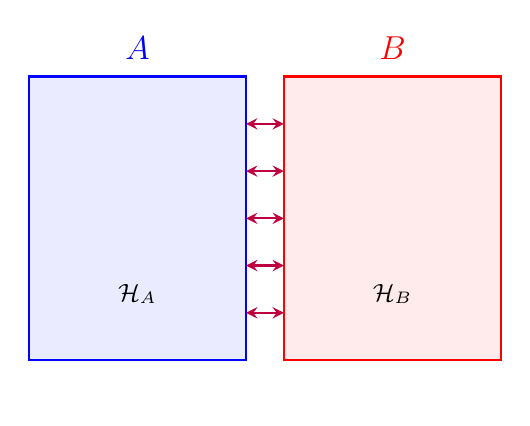
\begin{tikzpicture}[scale=1.2]
    % 画区域A
    \draw[thick, blue, fill=blue!8] (-2.5,-1.5) rectangle (-0.2,1.5);
    \node[blue, font=\large] at (-1.35, 1.8) {$A$};
    % 画区域B
    \draw[thick, red, fill=red!8] (0.2,-1.5) rectangle (2.5,1.5);
    \node[red, font=\large] at (1.35, 1.8) {$B$};
    % 纠缠连线
    \foreach \y in {-1.0,-0.5,0.0,0.5,1.0} {
        \draw[thick, purple, <->, >=stealth] (-0.2,\y) -- (0.2,\y);
    }
    \node[purple, font=\footnotesize] at (0, -1.8) {纠缠关联};
    % 标注Hilbert空间
    \node[font=\small] at (-1.35, -0.8) {$\mathcal{H}_A$};
    \node[font=\small] at (1.35, -0.8) {$\mathcal{H}_B$};
\end{tikzpicture}
\caption{纠缠系统示意图：子区域 $A$ 和 $B$ 构成总系统，它们通过量子纠缠（紫色连线）相关联。即使 $A$ 和 $B$ 空间分离，纠缠仍然存在。}
\label{fig:entangled_system}
\end{figure}

然而，大多数量子态不能写成这种可分形式。例如，考虑以下双量子比特态。

\begin{example}[贝尔态的纠缠]\label{ex:bell}
考虑贝尔态（Bell state）：
\begin{equation}\label{eq:bell_state}
    |\Psi^-\rangle = \frac{1}{\sqrt{2}}(|\uparrow\downarrow\rangle - |\downarrow\uparrow\rangle).
\end{equation}
我们证明这个状态不可分。假设存在 $|\psi_A\rangle = \alpha|\uparrow\rangle + \beta|\downarrow\rangle$ 和 $|\phi_B\rangle = \gamma|\uparrow\rangle + \delta|\downarrow\rangle$ 使得 $|\Psi^-\rangle = |\psi_A\rangle \otimes |\phi_B\rangle$，则
\begin{equation}
    |\psi_A\rangle \otimes |\phi_B\rangle = \alpha\gamma|\uparrow\uparrow\rangle + \alpha\delta|\uparrow\downarrow\rangle + \beta\gamma|\downarrow\uparrow\rangle + \beta\delta|\downarrow\downarrow\rangle.
\end{equation}
与~\eqref{eq:bell_state} 比较系数，必须满足 $\alpha\gamma = 0$、$\beta\delta = 0$、$\alpha\delta = 1/\sqrt{2}$、$\beta\gamma = -1/\sqrt{2}$。由 $\alpha\delta \neq 0$ 知 $\alpha \neq 0$ 且 $\delta \neq 0$，但由 $\alpha\gamma = 0$ 知 $\gamma = 0$，这与 $\beta\gamma = -1/\sqrt{2} \neq 0$ 矛盾。因此 $|\Psi^-\rangle$ 不可分，即为纠缠态。$\square$
\end{example}

四个贝尔态构成了双量子比特空间的一组正交归一基：
\begin{equation}
    |\Psi^\pm\rangle = \frac{1}{\sqrt{2}}(|\uparrow\downarrow\rangle \pm |\downarrow\uparrow\rangle), \quad
    |\Phi^\pm\rangle = \frac{1}{\sqrt{2}}(|\uparrow\uparrow\rangle \pm |\downarrow\downarrow\rangle).
\end{equation}

\begin{figure}[htbp]
\centering
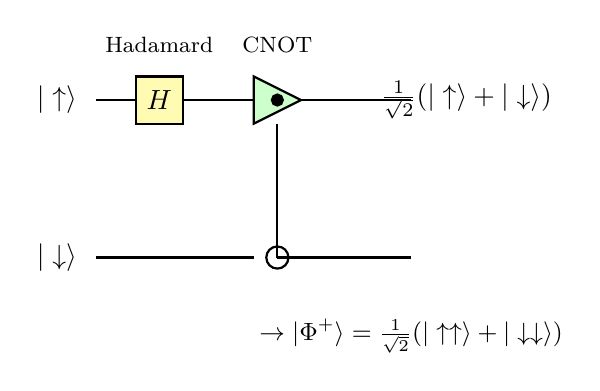
\begin{tikzpicture}[scale=1.0, >=stealth]
    % 输入态
    \node at (-1, 2) {$|\uparrow\rangle$};
    \node at (-1, 0) {$|\downarrow\rangle$};
    % 线
    \draw[thick] (-0.5, 2) -- (1.5, 2);
    \draw[thick] (-0.5, 0) -- (1.5, 0);
    % H gate
    \draw[thick, fill=yellow!30] (0, 1.7) rectangle (0.6, 2.3);
    \node at (0.3, 2) {$H$};
    % CNOT
    \draw[thick, fill=green!20] (1.5, 1.7) -- (2.1, 2) -- (1.5, 2.3) -- cycle;
    \filldraw (1.8, 2) circle (2pt);
    \draw[thick] (1.8, 0) -- (1.8, 1.7);
    \draw[thick] (1.8, 0) circle (4pt);
    % 输出
    \draw[thick] (2.1, 2) -- (3.5, 2);
    \draw[thick] (1.8, 0) -- (3.5, 0);
    \node at (4.2, 2) {$\frac{1}{\sqrt{2}}(|\uparrow\rangle + |\downarrow\rangle)$};
    \node at (4.2, 0) {条件翻转};
    % 结果
    \node[font=\small] at (3.5, -1) {$\to |\Phi^+\rangle = \frac{1}{\sqrt{2}}(|\uparrow\uparrow\rangle + |\downarrow\downarrow\rangle)$};
    % 标注
    \node[font=\footnotesize] at (0.3, 2.7) {Hadamard};
    \node[font=\footnotesize] at (1.8, 2.7) {CNOT};
\end{tikzpicture}
\caption{制备贝尔态 $|\Phi^+\rangle$ 的量子线路：先对第一个量子比特施加 Hadamard 门，再以第一个比特为控制比特施加 CNOT 门。}
\label{fig:bell_circuit}
\end{figure}

\begin{remark}
量子纠缠与经典关联有本质区别。经典关联（如将一副手套分寄两地）可以通过隐变量解释，而贝尔不等式的违反表明量子纠缠无法用任何局域隐变量理论描述。
\end{remark}

%=============================================================================
\section{约化密度矩阵与纠缠熵}
%=============================================================================

在量子力学中，当我们只关注复合系统的某个子系统时，描述该子系统状态的数学工具是约化密度矩阵。为了量化纠缠程度，我们需要引入这一概念并定义纠缠熵。

\begin{definition}[密度矩阵与约化密度矩阵]
对于一个纯态 $|\Psi\rangle$，总密度矩阵为 $\rho_{\rm tot} = |\Psi\rangle\langle\Psi|$。当我们只关注子系统 $A$ 时，需要对子系统 $B$ 求偏迹（partial trace），得到约化密度矩阵：
\begin{equation}\label{eq:reduced_dm}
    \rho_A = \Tr_B(\rho_{\rm tot}) = \sum_{i} {}_B\langle i | \rho_{\rm tot} | i\rangle_B,
\end{equation}
其中 $\{|i\rangle_B\}$ 是子系统 $B$ 的一组正交归一基。
\end{definition}

下面我们对贝尔态显式计算约化密度矩阵。

\begin{example}[贝尔态的约化密度矩阵]
对于贝尔态 $|\Psi^-\rangle = \frac{1}{\sqrt{2}}(|\uparrow\downarrow\rangle - |\downarrow\uparrow\rangle)$，总密度矩阵为
\begin{equation}
    \rho_{\rm tot} = \frac{1}{2}\big(|\uparrow\downarrow\rangle - |\downarrow\uparrow\rangle\big)\big(\langle\uparrow\downarrow| - \langle\downarrow\uparrow|\big).
\end{equation}
展开得到
\begin{equation}
    \rho_{\rm tot} = \frac{1}{2}\big(|\uparrow\downarrow\rangle\langle\uparrow\downarrow| - |\uparrow\downarrow\rangle\langle\downarrow\uparrow| - |\downarrow\uparrow\rangle\langle\uparrow\downarrow| + |\downarrow\uparrow\rangle\langle\downarrow\uparrow|\big).
\end{equation}
对 $B$ 求偏迹，取 $B$ 的基为 $\{|\uparrow\rangle_B, |\downarrow\rangle_B\}$：
\begin{align}
    \rho_A &= {}_B\langle\uparrow|\rho_{\rm tot}|\uparrow\rangle_B + {}_B\langle\downarrow|\rho_{\rm tot}|\downarrow\rangle_B \nonumber\\
    &= \frac{1}{2}|\downarrow\rangle\langle\downarrow| \cdot 1 + \frac{1}{2}|\uparrow\rangle\langle\uparrow| \cdot 1 \nonumber\\
    &= \frac{1}{2}\big(|\uparrow\rangle\langle\uparrow| + |\downarrow\rangle\langle\downarrow|\big) = \frac{1}{2}\mathbb{I}_A.
\end{align}
约化密度矩阵为最大混合态 $\frac{1}{2}\mathbb{I}_A$，这表明我们对子系统 $A$ 的状态完全"无知"——它处于最大纠缠状态。
\end{example}

约化密度矩阵 $\rho_A$ 的本征值分布反映了纠缠程度。如果系统是可分的，$\rho_A$ 是纯态，只有一个本征值为 1，其余为 0；如果系统是纠缠的，$\rho_A$ 是混合态，本征值分布更加均匀。

\begin{definition}[纠缠熵]\label{def:ee}
纠缠熵定义为约化密度矩阵的 von Neumann 熵：
\begin{equation}\label{eq:ee}
    S_A = -\Tr_A(\rho_A \ln \rho_A) = -\sum_i p_i \ln p_i,
\end{equation}
其中 $p_i$ 是 $\rho_A$ 的本征值。纠缠熵度量了子系统 $A$ 与子系统 $B$ 之间的纠缠程度。
\end{definition}

\begin{proof}
公式~\eqref{eq:ee} 的推导如下。设 $\rho_A$ 的谱分解为 $\rho_A = \sum_i p_i |e_i\rangle\langle e_i|$，则
\begin{equation}
    \ln \rho_A = \sum_i (\ln p_i) |e_i\rangle\langle e_i|,
\end{equation}
从而
\begin{equation}
    \rho_A \ln \rho_A = \sum_i p_i (\ln p_i) |e_i\rangle\langle e_i|,
\end{equation}
取迹得到
\begin{equation}
    \Tr_A(\rho_A \ln \rho_A) = \sum_i p_i \ln p_i.
\end{equation}
因此 $S_A = -\sum_i p_i \ln p_i$。这里使用自然对数 $\ln$，约定 $0 \ln 0 = 0$。
\end{proof}

\begin{note}[纠缠熵的物理意义]
纠缠熵可以被理解为"我们对子系统 $A$ 的无知程度"：
\begin{itemize}
    \item 如果系统是可分的，$\rho_A$ 为纯态，$S_A = 0$。
    \item 如果系统是纠缠的，$\rho_A$ 为混合态，$S_A > 0$。
    \item 纠缠熵越大，子系统之间的纠缠越强。
    \item 对于 $d$ 维希尔伯特空间中的最大混合态 $\rho_A = \frac{1}{d}\mathbb{I}$，纠缠熵取最大值 $S_{\max} = \ln d$。
\end{itemize}
\end{note}

\begin{example}[贝尔态的纠缠熵]
对于贝尔态，$\rho_A = \frac{1}{2}\mathbb{I}_A$，本征值为 $p_1 = p_2 = \frac{1}{2}$，因此
\begin{equation}
    S_A = -\frac{1}{2}\ln\frac{1}{2} - \frac{1}{2}\ln\frac{1}{2} = \ln 2.
\end{equation}
这正好是最大值 $S_{\max} = \ln 2$（对于二维希尔伯特空间），确认了贝尔态是最大纠缠态。
\end{example}

%=============================================================================
\section{纠缠熵的基本性质}
%=============================================================================

纠缠熵具有几个重要的数学性质。这些性质的证明依赖于密度矩阵的半正定性以及 von Neumann 熵的凹性等基本工具。

\begin{property}[基本性质]\label{prop:basic}
纠缠熵满足以下基本性质：
\begin{enumerate}
    \item \textbf{非负性}：$S_A \geq 0$，等号成立当且仅当 $\rho_A$ 为纯态。
    \item \textbf{对称性}：对于纯态 $|\Psi\rangle_{AB}$，$S_A = S_B$。
    \item \textbf{上界}：$S_A \leq \ln \dim\mathcal{H}_A$。
\end{enumerate}
\end{property}

\begin{proof}[对称性的证明]
对于纯态 $|\Psi\rangle_{AB}$，总密度矩阵满足 $\rho_{\rm tot}^2 = \rho_{\rm tot}$。设 $\rho_A$ 的谱分解为 $\rho_A = \sum_i p_i |a_i\rangle\langle a_i|$。将 $|\Psi\rangle$ 按 Schmidt 分解展开：
\begin{equation}
    |\Psi\rangle = \sum_i \sqrt{p_i}\, |a_i\rangle_A \otimes |b_i\rangle_B,
\end{equation}
其中 $\{|b_i\rangle_B\}$ 是 $B$ 的一组正交归一基。类似地计算 $\rho_B = \Tr_A(\rho_{\rm tot})$：
\begin{equation}
    \rho_B = \sum_i p_i |b_i\rangle\langle b_i|.
\end{equation}
$\rho_B$ 的本征值集合与 $\rho_A$ 相同，因此 $S_B = -\sum_i p_i \ln p_i = S_A$。
\end{proof}

下面讨论纠缠熵最重要的不等式——次可加性。

\begin{theorem}[次可加性]\label{thm:subadditivity}
对于复合系统 $ABC$ 的纯态，约化密度矩阵的 von Neumann 熵满足：
\begin{equation}\label{eq:subadditivity}
    S_{AB} \leq S_A + S_B,
\end{equation}
等号成立当且仅当 $A$ 和 $B$ 不纠缠（即 $\rho_{AB} = \rho_A \otimes \rho_B$）。
\end{theorem}

\begin{proof}
定义量子互信息（mutual information）$I(A:B) = S_A + S_B - S_{AB}$。我们证明 $I(A:B) \geq 0$。

考虑复合系统 $AB$，有
\begin{equation}
    I(A:B) = S_A + S_B - S_{AB} = \Tr(\rho_A \ln \rho_A) + \Tr(\rho_B \ln \rho_B) - \Tr(\rho_{AB} \ln \rho_{AB}).
\end{equation}
利用相对熵（Kullback-Leibler divergence）$D(\rho\|\sigma) = \Tr(\rho \ln \rho - \rho \ln \sigma) \geq 0$，取 $\sigma = \rho_A \otimes \rho_B$：
\begin{align}
    D(\rho_{AB} \| \rho_A \otimes \rho_B) &= \Tr(\rho_{AB} \ln \rho_{AB}) - \Tr(\rho_{AB} \ln(\rho_A \otimes \rho_B)) \nonumber\\
    &= -S_{AB} - \Tr(\rho_{AB}(\ln \rho_A \otimes \mathbb{I}_B + \mathbb{I}_A \otimes \ln \rho_B)) \nonumber\\
    &= -S_{AB} - \Tr(\rho_A \ln \rho_A) - \Tr(\rho_B \ln \rho_B) \nonumber\\
    &= -S_{AB} - S_A - S_B = -I(A:B) \geq 0,
\end{align}
这里我们使用了 Klein 不等式（相对熵的非负性）。因此 $I(A:B) \geq 0$，即 $S_{AB} \leq S_A + S_B$。

当 $I(A:B) = 0$ 时，$D(\rho_{AB}\|\rho_A \otimes \rho_B) = 0$，由相对熵的性质知 $\rho_{AB} = \rho_A \otimes \rho_B$，即 $A$ 与 $B$ 不纠缠。
\end{proof}

\begin{theorem}[强次可加性]\label{thm:strong_subadd}
对于复合系统 $ABCD$，von Neumann 熵满足强次可加性：
\begin{equation}
    S_{ABC} + S_B \leq S_{AB} + S_{BC}.
\end{equation}
等价地，对于三个子系统 $A$、$B$、$C$：
\begin{equation}\label{eq:strong_subadd}
    S_{A \cup C} + S_{B} \leq S_{A \cup B} + S_{B \cup C}.
\end{equation}
\end{theorem}

\begin{note}[强次可加性的物理意义]
强次可加性是纠缠熵最重要的不等式之一，它反映了量子纠缠的"单调性"：纠缠不会因为局部操作而增加。这个性质在量子信息理论中被称为"纠缠单调性"，是量子纠缠理论的基础。在 AdS/CFT 中，强次可加性与体空间的量子极端面的性质密切相关，是证明量子极端面公式~\cite{Engelhardt2015} 的关键工具。
\end{note}

%=============================================================================
\section{面积律与量子场论}
%=============================================================================

在量子场论中，纠缠熵的一个核心性质是面积律：纠缠熵正比于子区域边界的面积，而非子区域的体积。这一性质深刻地联系了量子信息与引力物理~\cite{Casini2017}。

\begin{theorem}[面积律]\label{thm:area_law}
在 $d$ 维时空的量子场论中，对于一个空间区域 $A$，纠缠熵满足面积律：
\begin{equation}\label{eq:area_law}
    S_A = c_1 \frac{\operatorname{Area}(\partial A)}{\epsilon^{d-2}} + c_2 \frac{\operatorname{Area}(\partial A)}{\epsilon^{d-4}} + \cdots + c_{d-2}\operatorname{Area}(\partial A) \ln\frac{1}{\epsilon} + O(\epsilon^0),
\end{equation}
其中 $\epsilon$ 是紫外截断（UV cutoff），$c_i$ 是与理论细节有关的常数，$\partial A$ 是区域 $A$ 的边界。
\end{theorem}

\begin{figure}[htbp]
\centering
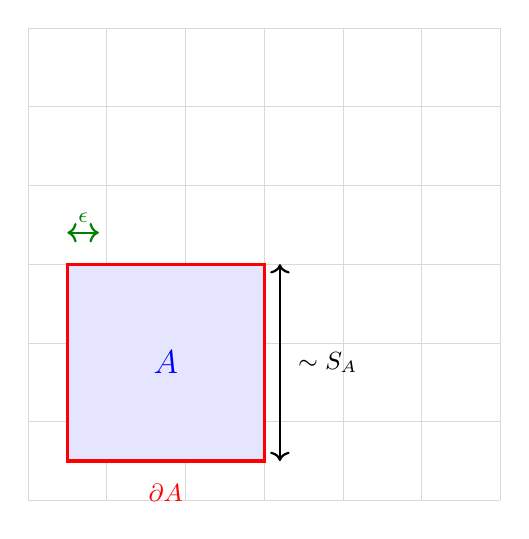
\begin{tikzpicture}[scale=1.0]
    % 网格（体区域）
    \draw[gray!30, very thin] (-3,-3) grid (3,3);
    % 区域A
    \draw[thick, blue, fill=blue!10] (-2.5,-2.5) rectangle (0,0);
    \node[blue, font=\large] at (-1.25, -1.25) {$A$};
    % 边界 partial A（加粗高亮）
    \draw[very thick, red] (-2.5, -2.5) -- (0, -2.5) -- (0, 0) -- (-2.5, 0) -- cycle;
    \node[red, font=\small] at (-1.25, -2.9) {$\partial A$};
    % 标注面积律
    \draw[<->, thick] (0.2, -2.5) -- (0.2, 0);
    \node[right, font=\small] at (0.3, -1.25) {$\sim S_A$};
    % 紫外截断
    \draw[thick, green!50!black, <->] (-2.5, 0.4) -- (-2.1, 0.4);
    \node[above, font=\footnotesize, green!50!black] at (-2.3, 0.4) {$\epsilon$};
\end{tikzpicture}
\caption{面积律示意图：纠缠熵 $S_A$ 正比于区域 $A$ 的边界 $\partial A$ 的面积（红色粗线），而非区域 $A$ 的体积。$\epsilon$ 为晶格间距或紫外截断。}
\label{fig:area_law}
\end{figure}

下面我们以自由标量场论为例，给出面积律的一个具体证明思路~\cite{Casini2017}。

\begin{proof}[自由标量场论中面积律的证明（概要）]
考虑 $d$ 维时空中自由实标量场 $\phi(x)$，空间为 $\mathbb{R}^{d-1}$，将空间分为区域 $A$ 和其补集 $\bar{A}$。

\textbf{第一步：等时关联函数。}自由场的等时关联函数为
\begin{equation}
    \langle\phi(\mathbf{x})\phi(\mathbf{y})\rangle = C(\mathbf{x}-\mathbf{y}) = \int \frac{d^{d-2}k}{(2\pi)^{d-2}} \frac{1}{2|\mathbf{k}|} e^{i\mathbf{k}\cdot(\mathbf{x}-\mathbf{y})},
\end{equation}
其中 $|\mathbf{k}| = \sqrt{k_1^2 + \cdots + k_{d-2}^2 + m^2}$。

\textbf{第二步：关联矩阵。}定义关联矩阵 $C_{AB}$，其元素为 $C_{ij} = C(\mathbf{x}_i - \mathbf{y}_j)$，其中 $\mathbf{x}_i \in A$，$\mathbf{y}_j \in A$。纠缠熵可以通过关联矩阵的本征值 $\lambda_i$ 来表达。

\textbf{第三步：纠缠熵公式。}对于高斯态，纠缠熵为
\begin{equation}
    S_A = \sum_i \left[\left(\lambda_i + \frac{1}{2}\right)\ln\left(\lambda_i + \frac{1}{2}\right) - \left(\lambda_i - \frac{1}{2}\right)\ln\left(\lambda_i - \frac{1}{2}\right)\right].
\end{equation}

\textbf{第四步：面积律的出现。}关联函数 $C(\mathbf{x}-\mathbf{y})$ 在 $\mathbf{x} \to \mathbf{y}$ 时有短距离发散 $\sim |\mathbf{x}-\mathbf{y}|^{-(d-2)}$。这一发散仅在边界 $\partial A$ 附近的点对 $(\mathbf{x}_i, \mathbf{y}_j)$ 产生主要贡献（当 $\mathbf{x}_i$ 和 $\mathbf{y}_j$ 分别位于 $A$ 和 $\bar{A}$ 时）。因此，求和的主要贡献来自边界附近的模式，给出
\begin{equation}
    S_A \sim \frac{\operatorname{Area}(\partial A)}{\epsilon^{d-2}}.
\end{equation}
这完成了面积律的证明概要。
\end{proof}

\begin{remark}
面积律的物理直观是：纠缠主要由边界附近的短程关联贡献。远离边界的内部模式对 $A$ 和 $\bar{A}$ 的关联没有净贡献，因为它们在两边对称地衰减。这一图像与凝聚态物理中一维系统的面积律（对数修正）~\cite{Calabrese2004} 一致。
\end{remark}

%=============================================================================
\section{Rényi 熵与纠缠熵的计算}
%=============================================================================

在实际计算中，直接计算 von Neumann 熵通常比较困难。一个更方便的工具是 Rényi 熵，它通过 replica trick 将熵的计算转化为配分函数的计算。

\begin{definition}[Rényi 熵]\label{def:renyi}
Rényi 熵定义为：
\begin{equation}\label{eq:renyi}
    S_n = \frac{1}{1-n} \ln \Tr_A(\rho_A^n),
\end{equation}
其中 $n$ 是正整数。
\end{definition}

\begin{proof}[Rényi 熵与 von Neumann 熵的关系]
当 $n \to 1$ 时，Rényi 熵趋于 von Neumann 熵。设 $\rho_A$ 的本征值为 $\{p_i\}$，则
\begin{equation}
    \Tr_A(\rho_A^n) = \sum_i p_i^n.
\end{equation}
当 $n \to 1$ 时，令 $n = 1 + \delta$，$\delta \to 0$：
\begin{align}
    \Tr_A(\rho_A^{1+\delta}) &= \sum_i p_i^{1+\delta} = \sum_i p_i \cdot p_i^\delta = \sum_i p_i \cdot e^{\delta \ln p_i} \nonumber\\
    &= \sum_i p_i(1 + \delta \ln p_i + O(\delta^2)) = 1 + \delta \sum_i p_i \ln p_i + O(\delta^2).
\end{align}
因此
\begin{equation}
    S_n = \frac{1}{1-n}\ln\Tr_A(\rho_A^n) = \frac{1}{-\delta}\ln\left(1 + \delta\sum_i p_i \ln p_i + O(\delta^2)\right) \to -\sum_i p_i \ln p_i = S.
\end{equation}
\end{proof}

Rényi 熵的一个重要性质是关于 $n$ 的单调性。

\begin{property}[Rényi 熵的单调性]
对于 $m > n \geq 1$，有 $S_m \leq S_n$。特别地，$S_1 = S \leq S_n$ 对所有 $n > 1$ 成立。
\end{property}

\begin{proof}
这是 Hölder 不等式的一个直接推论。定义 $f(n) = \frac{1}{1-n}\ln\Tr(\rho^n)$，可以证明 $\frac{df}{dn} \leq 0$。
\end{proof}

%=============================================================================
\section{纠缠熵与配分函数的联系}
%=============================================================================

纠缠熵可以通过配分函数来表达，这一联系在 AdS/CFT 对偶中至关重要，它将 von Neumann 熵的计算转化为复流形上路径积分的计算。

\begin{definition}[$n$ 叶黎曼面]
$n$ 叶黎曼面 $\Sigma_n$ 是一个由 $n$ 份时空副本沿着子区域 $A$ 的世界片（worldsheet）粘合而成的复流形。在 $A$ 的边界 $\partial A$ 处，副本按循环方式连接：第 $k$ 叶的 $A$ 区域与第 $k+1$ 叶的 $A$ 区域相连（$k = 1, \ldots, n$，模 $n$）。
\end{definition}

\begin{theorem}[纠缠熵与配分函数的联系]\label{thm:partition_function}
考虑 $n$ 叶黎曼面 $\Sigma_n$ 上的配分函数 $Z_n$。Rényi 熵可以写为：
\begin{equation}\label{eq:renyi_partition}
    S_n = \frac{1}{1-n} \ln \frac{Z_n}{Z_1^n},
\end{equation}
其中 $Z_1$ 是通常的配分函数。
\end{theorem}

\begin{proof}
$\Tr_A(\rho_A^n)$ 可以理解为在 $n$ 个副本之间"循环"地传播场构型。在路径积分语言中，这对应于在 $n$ 叶黎曼面上计算配分函数。具体地：
\begin{equation}
    \Tr_A(\rho_A^n) = \frac{Z_n}{Z_1^n},
\end{equation}
其中分母 $Z_1^n$ 是归一化因子，确保 $\Tr(\rho_A) = 1$。代入 Rényi 熵的定义~\eqref{eq:renyi}，得到~\eqref{eq:renyi_partition}。
\end{proof}

\begin{note}[物理意义]
这个联系的物理意义是：纠缠熵可以通过计算复几何上的配分函数来得到。在 AdS/CFT 对偶中，$n$ 叶黎曼面 $\Sigma_n$ 作为边界条件，对应于体空间中的某种复几何。通过 saddle point 近似，$Z_n$ 由体空间中的经典解主导，这为全息纠缠熵的计算提供了基础。
\end{note}

取 $n \to 1$ 极限，von Neumann 熵为
\begin{equation}
    S = -\left.\frac{\partial}{\partial n}\right|_{n=1} \ln \frac{Z_n}{Z_1^n} = -\left.\frac{\partial}{\partial n}\right|_{n=1} \ln Z_n + \ln Z_1.
\end{equation}

%=============================================================================
\section{全息纠缠熵}
%=============================================================================

AdS/CFT 对偶中，纠缠熵有一个深刻的几何解释。Ryu 和 Takayanagi 在 2006 年提出了一个著名的公式~\cite{Ryu2006}，将边界场论的纠缠熵与体空间中的极小曲面面积联系起来。

\begin{theorem}[Ryu-Takayanagi 公式]\label{thm:RT}
设 $A$ 是共形场论边界上的一个空间区域，$\gamma_A$ 是体空间中以 $\partial A$ 为边界的极小曲面（即面积泛函的临界点）。则区域 $A$ 的纠缠熵为：
\begin{equation}\label{eq:RT}
    S_A = \frac{\operatorname{Area}(\gamma_A)}{4G_N},
\end{equation}
其中 $G_N$ 是体空间中的牛顿引力常数。
\end{theorem}

\begin{remark}
Ryu-Takayanagi 公式~\eqref{eq:RT} 与黑洞熵的 Bekenstein-Hawking 公式 $S = A/(4G_N)$ 在形式上完全一致。这暗示纠缠熵与引力之间存在深刻的联系。
\end{remark}

RT 公式的证明需要利用~\eqref{eq:renyi_partition} 以及 AdS/CFT 中配分函数的引力对偶。当 $n \to 1$ 时，$n$ 叶黎曼面的引力配分函数由一个以 $\gamma_A$ 为固定边界的极值面主导，其作用量正比于 $\operatorname{Area}(\gamma_A)/(4G_N)$。

\begin{definition}[纠缠楔]
设 $\gamma_A$ 是体空间中的极小曲面，$\gamma_A$ 与边界区域 $A$ 共同围成的体空间区域 $\mathcal{W}_A$ 称为区域 $A$ 的\textbf{纠缠楔}（entanglement wedge）。
\end{definition}

\begin{figure}[htbp]
\centering
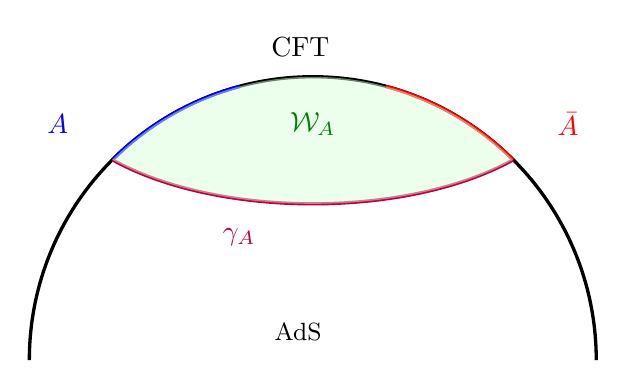
\begin{tikzpicture}[scale=1.2]
    % AdS边界
    \draw[very thick] (-3,0) arc (180:0:3);
    \node[above] at (0,3.1) {CFT 边界};
    % 区域A
    \draw[very thick, blue] (-2.12, 2.12) arc (135:105:3);
    \node[blue] at (-2.7, 2.5) {$A$};
    % 区域B的补
    \draw[very thick, red] (2.12, 2.12) arc (45:75:3);
    \node[red] at (2.7, 2.5) {$\bar{A}$};
    % 极小曲面 gamma_A
    \draw[very thick, purple] (-2.12, 2.12) .. controls (-1, 1.5) and (1, 1.5) .. (2.12, 2.12);
    \node[purple, left] at (-0.5, 1.3) {$\gamma_A$};
    % 纠缠楔（阴影）
    \fill[green!15, opacity=0.5] (-2.12, 2.12) .. controls (-1, 1.5) and (1, 1.5) .. (2.12, 2.12) arc (45:135:3);
    \node[green!50!black] at (0, 2.5) {$\mathcal{W}_A$};
    % 标注
    \node[font=\small] at (0, 0.3) {AdS 体空间};
\end{tikzpicture}
\caption{Ryu-Takayanagi 公式示意图：边界区域 $A$ 的纠缠熵由体空间中极小曲面 $\gamma_A$（紫色）的面积决定。$\gamma_A$ 与 $A$ 围成的区域 $\mathcal{W}_A$（绿色阴影）为纠缠楔。}
\label{fig:RT}
\end{figure}

\begin{theorem}[量子极端面公式]\label{thm:QES}
RT 公式在量子修正下推广为量子极端面（quantum extremal surface, QES）公式：
\begin{equation}\label{eq:QES}
    S_A = \min_{X \supset \partial A} \operatorname{ext}_X \left[\frac{\operatorname{Area}(X)}{4G_N} + S_{\rm bulk}(\Sigma_X)\right],
\end{equation}
其中 $X$ 是候选的极端面，$S_{\rm bulk}(\Sigma_X)$ 是体空间区域 $\Sigma_X$ 中物质场的 von Neumann 熵，$\operatorname{ext}_X$ 表示对 $X$ 取极值。
\end{theorem}

\begin{note}
量子极端面公式~\eqref{eq:QES} 是近年来黑洞信息悖论研究的核心工具。Page 曲线的全息推导正是基于这一公式。
\end{note}

%=============================================================================
\section{纠缠熵在物理学中的应用}
%=============================================================================

纠缠熵在现代物理学中有着广泛而深刻的应用，下面列出几个主要方向。

\begin{example}[ER = EPR 猜想]
Van Raamsdonk~\cite{VanRaamsdonk2010} 指出，量子纠缠与时空连通性密切相关。如果两个 CFT 处于纠缠态 $\rho_{AB}$，则它们的 AdS 对偶体空间通过 Einstein-Rosen 桥（虫洞）相连。当纠缠消失时（$S_A \to 0$），虫洞断开，时空分离。Maldacena 和 Susskind 将此推广为 ER = EPR 猜想：Einstein-Rosen 桥等价于 Einstein-Podolsky-Rosen 纠缠。
\end{example}

\begin{definition}[量子纠错码与纠缠楔]
在 AdS/CFT 中，体空间局域算子 $\mathcal{O}(x)$ 可以用边界 CFT 的算子表示。如果 $x$ 位于区域 $A$ 的纠缠楔 $\mathcal{W}_A$ 内，则 $\mathcal{O}(x)$ 可以由区域 $A$ 上的算子重构。这本质上是一种量子纠错码的结构：体空间信息被"编码"在边界子系统中，即使部分边界信息丢失，只要 $A$ 足够大，体空间信息仍可恢复。
\end{definition}

\begin{itemize}
    \item \textbf{量子信息}：纠缠熵是量化量子纠缠的基本工具，它在量子计算、量子通信和量子密码学中都有重要应用。
    \item \textbf{凝聚态物理}：纠缠熵可以用来区分不同的量子相，例如拓扑相的长程纠缠和量子临界点的对数修正面积律~\cite{Calabrese2004}。
    \item \textbf{高能物理}：纠缠熵在黑洞物理和 AdS/CFT 对偶中扮演着核心角色，RT 公式和量子极端面公式是全息理论的基石~\cite{Ryu2006}。
    \item \textbf{量子引力}：纠缠熵为理解时空的本质提供了新视角。Van Raamsdonk~\cite{VanRaamsdonk2010} 指出，时空本身可能由量子纠缠"编织"而成。
\end{itemize}

\begin{remark}[纠缠熵与全息重正化]
在 AdS/CFT 中，纠缠熵的 UV 发散与全息重正化（holographic renormalization）密切相关。RT 公式中的极小曲面面积包含了与 CFT 中面积律发散相对应的发散项。通过适当的重正化方案，可以提取出有限的纠缠熵，这为研究 CFT 的中心荷和共形反常提供了新方法。
\end{remark}

%=============================================================================
\section{量子场论中纠缠熵的具体计算}
%=============================================================================

为了加深理解，我们给出两个具体计算纠缠熵的示例。

\begin{example}[二维 CFT 中的纠缠熵]\label{ex:2d_CFT}
在二维共形场论中，纠缠熵有精确结果。考虑圆环上的 CFT，区域 $A$ 为长度为 $\ell$ 的区间。在圆环上（温度 $T = 1/\beta$），纠缠熵为~\cite{Calabrese2004}：
\begin{equation}
    S_A = \frac{c}{3} \ln\left[\frac{\beta}{\pi\epsilon}\sinh\left(\frac{\pi\ell}{\beta}\right)\right],
\end{equation}
其中 $c$ 是中心荷。

\textbf{推导：}在 $n$ 叶黎曼面 $\Sigma_n$ 上，共形映射 $w \to z = w^{1/n}$ 将 $\Sigma_n$ 映到单叶复平面。配分函数比值为
\begin{equation}
    \frac{Z_n}{Z_1^n} = \left|\frac{\partial z}{\partial w}\right|^{c/6} \cdot (\text{共形因子贡献}) = \left[\frac{\beta}{\pi\epsilon}\sinh\left(\frac{\pi\ell}{\beta}\right)\right]^{c(1-n)/6n} \cdot \text{(修正项)}.
\end{equation}
取 $\ln$ 并除以 $1-n$，令 $n \to 1$，得到上述结果。注意当 $\ell \ll \beta$ 时，$S_A \approx \frac{c}{3}\ln\frac{\ell}{\epsilon}$，即零温结果；当 $\ell \gg \beta$ 时，$S_A \approx \frac{c\pi\ell}{3\beta}$，即体积律（有限温度效应）。
\end{example}

\begin{example}[自由费米子的纠缠熵]
考虑 $(1+1)$ 维自由 Dirac 费米子，基态下长度为 $L$ 的区间 $A$ 的纠缠熵为：
\begin{equation}
    S_A = \frac{1}{3}\ln\frac{L}{\epsilon} + \text{const}.
\end{equation}
这里中心荷 $c = 1$（单个 Dirac 费米子相当于两个 Majorana 费米子，每个 $c = 1/2$）。这一结果可以通过关联矩阵的方法计算：定义等时两点函数 $C_{ij} = \langle\psi^\dagger(x_i)\psi(x_j)\rangle$，纠缠熵由 $C$ 的本征值 $\{\lambda_i\}$ 给出：
\begin{equation}
    S_A = -\sum_i \left[\lambda_i \ln \lambda_i + (1-\lambda_i)\ln(1-\lambda_i)\right].
\end{equation}
对于连续谱，本征值分布趋于阶梯函数，求和变为积分，最终给出对数发散。
\end{example}

\begin{note}[纠缠熵与中心荷]
在二维 CFT 中，$\frac{c}{3}\ln\frac{L}{\epsilon}$ 这一对数发散项的系数直接给出中心荷 $c$。这使得纠缠熵成为一种"纠缠谱探测器"，可以通过测量纠缠熵来确定 CFT 的中心荷，而无需知道场论的具体内容。在 AdS/CFT 中，中心荷 $c$ 与 AdS 半径 $L_{\rm AdS}$ 和牛顿常数 $G_N$ 的关系为 $c = \frac{3L_{\rm AdS}}{2G_N}$。
\end{note}

%=============================================================================
\section{纠缠熵与量子引力的前沿}
%=============================================================================

近年来，纠缠熵在量子引力研究中取得了突破性进展，尤其体现在以下几个方面。

\begin{itemize}
    \item \textbf{量子极端面与 Page 曲线}：利用量子极端面公式~\eqref{eq:QES}，可以计算蒸发中黑洞的纠缠熵。结果表明，黑洞的 Page 曲线在半经典近似下可以得到正确恢复，这为解决黑洞信息悖论提供了重要线索。

    \item \textbf{岛屿公式}：在量子极端面公式的基础上，引力路径积分中的"岛"（island）贡献被发现。有效 Page 时间后的纠缠熵为
    \begin{equation}
        S(\text{辐射}) = \min\left\{\operatorname{ext}\left[\frac{\operatorname{Area}(\partial I)}{4G_N} + S_{\rm bulk}(\text{辐射} \cup I)\right]\right\},
    \end{equation}
    其中 $I$ 是黑洞内部的一个"岛"区域。这一公式在 Page 时间后自动给出正确的纠缠熵，确保了幺正性。

    \item \textbf{量子纠错与体空间重构}：AdS/CFT 中的纠缠楔重构可以理解为量子纠错码。边界 CFT 子区域 $A$ 上的算子代数可以编码体空间纠缠楔 $\mathcal{W}_A$ 中的信息。这一结构由 Almheiri、Dong 和 Harlow~\cite{Almheiri2015} 首次系统研究，揭示了全息对偶与量子信息论之间的深层联系。
\end{itemize}

\begin{remark}
纠缠熵已经成为连接量子引力、量子信息和高能物理的桥梁。从 Ryu-Takayanagi 公式到量子极端面公式，再到岛屿公式，每一次进展都深化了我们对时空本质的理解。正如 Van Raamsdonk~\cite{VanRaamsdonk2010} 所指出的，量子纠缠可能是构建时空几何的基本"线程"。
\end{remark}


\chapter{全息纠缠熵 (Holographic Entanglement Entropy)}

%=============================================================================
%
% 全息纠缠熵
%

在上一节中，我们介绍了纠缠熵的基本概念。我们知道，纠缠熵度量量子系统中子系统之间的纠缠程度，并且在量子场论中，纠缠熵满足面积律：$S_A \sim \text{Area}(\partial A)/\epsilon^{d-2}$。这个面积律与黑洞熵的贝肯斯坦-霍金公式 $S = A/(4G_N)$ 有着惊人的相似性。这种相似性并非巧合，它暗示着量子纠缠与引力几何之间存在深刻的联系。

2006 年，Ryu 和 Takayanagi 提出了一个革命性的公式 \cite{Ryu2006}，将这种联系精确化：边界 CFT 中区域 $A$ 的纠缠熵等于体空间 AdS 中以 $A$ 为边界的极小曲面的面积除以 $4G_N$。这个公式不仅提供了一个具体的计算方法，更揭示了量子信息与引力几何之间的深刻联系，成为 AdS/CFT 对偶中最重要的结果之一。

\section{极小曲面与纠缠熵公式}

考虑 AdS/CFT 对偶的设置：$(d+1)$ 维 AdS 空间中的引力理论对偶于 $d$ 维边界上的共形场论。在边界 CFT 中，考虑一个空间区域 $A$，我们想要计算区域 $A$ 与其补集 $\bar{A}$ 之间的纠缠熵。

在量子力学中，纠缠熵来源于复合系统量子态的不可分解性。当我们对复合系统的部分自由度求迹时，纯态变成混合态，纠缠熵正是度量这种纯度损失的量。在量子场论中，真空态虽然整体是纯态，但对于空间子区域而言，约化密度矩阵一般是非平凡的混合态，因此真空纠缠熵不为零。

\begin{definition}[量子纠缠]
量子纠缠是量子力学中最基本的非经典关联。对于一个由两个子系统 $A$ 和 $B$ 组成的复合系统，如果其量子态 $|\Psi\rangle_{AB}$ 不能写成子系统态的直积形式 $|\psi\rangle_A \otimes |\phi\rangle_B$，则称该态为纠缠态。纠缠熵 $S_A = -\text{tr}(\rho_A \ln \rho_A)$ 定量地度量了这种纠缠的程度，其中 $\rho_A = \text{tr}_B |\Psi\rangle\langle\Psi|$ 是子系统 $A$ 的约化密度矩阵。
\end{definition}

\begin{remark}[面积律的物理起源]
量子场论中纠缠熵的面积律 $S_A \sim \text{Area}(\partial A)/\epsilon^{d-2}$ 暗示着纠缠主要发生在区域边界附近。这是因为量子场的短程关联主导了纠缠的贡献，而短程关联只在区域边界处对纠缠有非零贡献。这个面积律与黑洞熵的贝肯斯坦-霍金公式 $S_{\text{BH}} = A/(4G_N)$ 具有相同的结构，暗示着引力与量子纠缠之间存在深层联系。
\end{remark}

\begin{theorem}[极小曲面与纠缠熵公式] \label{thm:RT}
Ryu 和 Takayanagi 提出 \cite{Ryu2006}，纠缠熵由以下公式给出：
\begin{equation}
    S_A = \frac{\text{Area}(\gamma_A)}{4 G_N},
    \label{eq:RT}
\end{equation}
其中 $\gamma_A$ 是 AdS 空间中满足以下条件的曲面：
\begin{enumerate}
    \item $\gamma_A$ 的边界与区域 $A$ 的边界相同：$\partial \gamma_A = \partial A$
    \item $\gamma_A$ 是极小曲面，即在所有满足条件 1 的曲面中，$\gamma_A$ 的面积最小
    \item $\gamma_A$ 位于体空间内部，不与边界相交（除了在 $\partial A$ 处）
\end{enumerate}
\end{theorem}

\begin{definition}[极小曲面]
在所有以给定边界为边界的曲面中，面积最小的曲面称为\textbf{极小曲面}（minimal surface）。在数学上，极小曲面满足平均曲率为零的条件：$H = 0$。在 AdS 空间中，由于负曲率的存在，极小曲面会向体空间内部弯曲，就像一个肥皂膜在弯曲的铁丝圈上形成的形状。
\end{definition}

\begin{remark}[极小曲面方程的推导]
极小曲面方程可以从面积泛函的变分得到。对于参数化曲面 $X^\mu(\sigma^1, \sigma^2)$，面积泛函为：
\begin{equation}
    \mathcal{A}[X] = \int d^2\sigma \sqrt{\det h_{ab}},
\end{equation}
其中 $h_{ab} = G_{\mu\nu} \partial_a X^\mu \partial_b X^\nu$ 是诱导度规。对 $X^\mu$ 变分并令 $\delta \mathcal{A} = 0$，得到极小曲面方程：
\begin{equation}
    \frac{1}{\sqrt{\det h}} \partial_a \left( \sqrt{\det h} \, h^{ab} \partial_b X^\mu \right) + \Gamma^\mu_{\rho\sigma} h^{ab} \partial_a X^\rho \partial_b X^\sigma = 0,
\end{equation}
其中 $\Gamma^\mu_{\rho\sigma}$ 是背景度规 $G_{\mu\nu}$ 的 Christoffel 符号。这个方程的几何意义是：曲面的平均曲率向量为零，即 $H^\mu = 0$。
\end{remark}

\begin{remark}[与黑洞熵的类比]
这个公式与黑洞熵的贝肯斯坦-霍金公式 $S = A/(4G_N)$ 非常相似。在黑洞的情况下，$A$ 是视界的面积；在全息纠缠熵的情况下，$A$ 是极小曲面的面积。这种相似性暗示着纠缠熵与引力之间存在深刻的联系。
\end{remark}

\begin{property}[极小曲面与纠缠熵公式的基本性质]
极小曲面与纠缠熵公式具有以下重要性质：
\begin{enumerate}
    \item \textbf{面积律}：对于边界区域 $A$，纠缠熵正比于其边界 $\partial A$ 的面积，这与量子场论中的面积律一致。
    \item \textbf{次可加性}：对于任意两个区域 $A$ 和 $B$，纠缠熵满足次可加性不等式 $S_{A \cup B} \leq S_A + S_B$。
    \item \textbf{强次可加性}：对于任意三个区域 $A$、$B$、$C$，纠缠熵满足强次可加性 $S_{A \cup B} + S_{B \cup C} \geq S_A + S_C$。
    \item \textbf{单调性}：在重整化群流下，纠缠熵单调递减，这与 $c$-定理和 $F$-定理一致。
\end{enumerate}
这些性质在全息框架下可以从极小曲面的几何性质自然推导出来。
\end{property}

图 \ref{fig:RT} 展示了极小曲面与纠缠熵公式的示意图。

\begin{figure}[htbp]
\centering
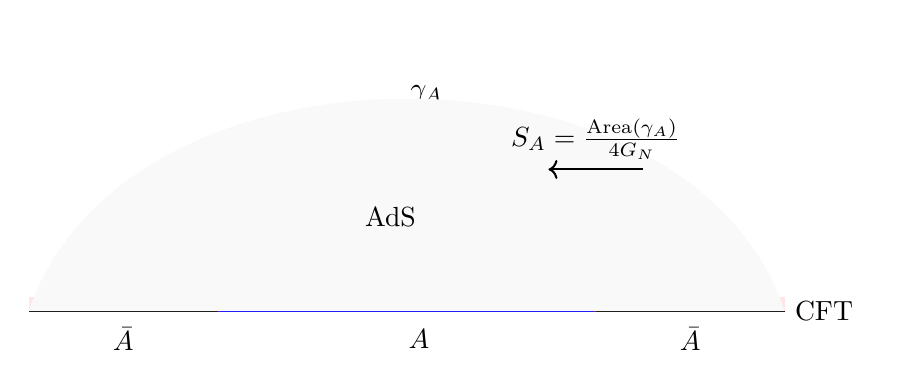
\begin{tikzpicture}[scale=1.2]
    % 绘制边界
    \draw[thick] (-4,0) -- (4,0) node[right] {CFT 边界};

    % 绘制区域 A 和 A_bar
    \fill[blue!20] (-2,0) -- (2,0) -- (2,0.15) -- (-2,0.15) -- cycle;
    \draw[thick, blue] (-2,0) -- (2,0);
    \node at (0,-0.3) {区域 $A$};

    \fill[red!10] (-4,0) -- (-2,0) -- (-2,0.15) -- (-4,0.15) -- cycle;
    \fill[red!10] (2,0) -- (4,0) -- (4,0.15) -- (2,0.15) -- cycle;
    \node at (-3,-0.3) {$\bar{A}$};
    \node at (3,-0.3) {$\bar{A}$};

    % 绘制极小曲面
    \draw[red, very thick] (-2,0) .. controls (-1.5,2) and (1.5,2) .. (2,0);
    \node at (0,2.3) {极小曲面 $\gamma_A$};

    % 绘制体空间
    \fill[gray!5] (-4,0) .. controls (-3,3) and (3,3) .. (4,0) -- cycle;
    \node at (0,1) {AdS 体空间};

    % 标注公式
    \draw[->] (2.5,1.5) -- (1.5,1.5) node[midway, above] {$S_A = \frac{\text{Area}(\gamma_A)}{4G_N}$};
\end{tikzpicture}
\caption{极小曲面与纠缠熵公式示意图。边界区域 $A$ 的纠缠熵由 AdS 体空间中以 $A$ 为边界的极小曲面 $\gamma_A$ 的面积除以 $4G_N$ 给出。}
\label{fig:RT}
\end{figure}

\begin{note}[物理意义]
极小曲面与纠缠熵公式告诉我们，边界 CFT 中的量子纠缠可以用体空间中的几何来描述。纠缠越多，极小曲面的面积越大，曲面越深入体空间内部。这提供了一个"几何化"量子纠缠的方法。
\end{note}

\begin{note}[适用条件]
极小曲面与纠缠熵公式在以下条件下成立：
\begin{enumerate}
    \item 经典引力极限：$G_N \to 0$，即 $N \to \infty$ 且 $\lambda = g_{YM}^2 N \to \infty$
    \item 稳态背景：时空是静态的或准静态的
    \item 无高阶导数修正：引力作用量是 Einstein-Hilbert 作用量
\end{enumerate}
当这些条件不满足时，需要对公式进行推广，例如量子极小曲面公式和含时纠缠熵公式。
\end{note}

\begin{remark}[RT 公式的物理意义]
Ryu-Takayanagi 公式 \cite{Ryu2006} 的核心物理意义在于：它表明边界 CFT 中的量子纠缠结构完全编码在体空间的几何之中。纠缠熵正比于极小曲面的面积，这意味着纠缠越多的区域，其对应的极小曲面越深入体空间内部。这一对应关系暗示着 AdS 空间的几何结构本质上由边界理论的量子纠缠所决定。换言之，如果移除边界 CFT 中的纠缠，体空间中的连通性也将被破坏——时空本身是量子纠缠的"涌现"产物。
\end{remark}

\section{公式的推导思路}

极小曲面与纠缠熵公式可以从 Replica trick 和 AdS/CFT 对偶推导出来。推导的关键思想是：纠缠熵可以通过 Rényi 熵的极限 $n \to 1$ 得到，而 Rényi 熵可以通过计算 $n$ 叶黎曼面上的配分函数得到。

\begin{definition}[Rényi 熵]
Rényi 熵是纠缠熵的推广，定义为：
\begin{equation}
    S_n = \frac{1}{1-n} \ln \text{tr}(\rho_A^n),
\end{equation}
其中 $n$ 是正整数，$\rho_A$ 是子系统 $A$ 的约化密度矩阵。当 $n \to 1$ 时，Rényi 熵还原为 von Neumann 纠缠熵：$S = \lim_{n \to 1} S_n = -\text{tr}(\rho_A \ln \rho_A)$。
\end{definition}

\begin{remark}[Rényi 熵的物理意义]
Rényi 熵的物理意义是：它度量了系统在不同精度下的纠缠程度，$n$ 越大，对高纠缠态的惩罚越重。在 AdS/CFT 对偶中，Rényi 熵的引力对偶由 Dong 于 2016 年给出 \cite{Dong2016}，其中 $n$ 叶覆盖空间中的引力作用量直接给出 $\text{tr}(\rho_A^n)$ 的对偶描述。
\end{remark}

考虑 $n$ 个复制品的系统，边界 CFT 的 Rényi 熵为：
\begin{equation}
    S_n = \frac{1}{1-n} \ln \frac{Z_n}{Z_1^n},
\end{equation}
其中 $Z_n$ 是 $n$ 叶黎曼面上的配分函数，$Z_1$ 是通常的配分函数。

在 AdS/CFT 对偶中，$Z_n$ 可以通过计算体空间中的引力配分函数得到。当 $n$ 为整数时，体空间是一个 $n$ 叶覆盖空间，其边界是 $n$ 叶黎曼面。通过计算这个空间的引力作用量，可以得到 $Z_n$。

\begin{theorem}[Lewkowycz-Maldacena 推导] \label{thm:Lewkowycz}
Lewkowycz 和 Maldacena 于 2013 年给出了极小曲面与纠缠熵公式的严格推导 \cite{Lewkowycz2013}。他们的推导基于以下关键步骤：
\begin{enumerate}
    \item 利用 Replica trick 将纠缠熵表示为 Rényi 熵的极限
    \item 在 AdS/CFT 对偶中，Rényi 熵对应于体空间中的锥形奇异点
    \item 通过引力作用量的变分，证明极小曲面条件自然出现
\end{enumerate}
\end{theorem}

\begin{proof}[极小曲面与纠缠熵公式的推导]
我们按照 Lewkowycz-Maldacena 的方法推导极小曲面与纠缠熵公式。考虑边界 CFT 中区域 $A$ 的 Rényi 熵：
\begin{equation}
    S_n = \frac{1}{1-n} \ln \frac{Z_n}{Z_1^n}.
\end{equation}

在 AdS/CFT 对偶中，边界 CFT 的配分函数等于体空间中的引力配分函数：
\begin{equation}
    Z_{\text{CFT}} = Z_{\text{grav}} = e^{-I_{\text{grav}}},
\end{equation}
其中 $I_{\text{grav}}$ 是引力作用量。

对于 $n$ 叶覆盖空间，体空间是一个锥形流形，在极小曲面 $\gamma_A$ 处有一个锥形奇异点，其亏格为 $n$。引力作用量可以分解为：
\begin{equation}
    I_{\text{grav}}^{(n)} = I_{\text{bulk}}^{(n)} + I_{\text{boundary}}^{(n)},
\end{equation}
其中 $I_{\text{bulk}}^{(n)}$ 是体空间的作用量，$I_{\text{boundary}}^{(n)}$ 是边界项。

关键的观察是：在 $n \to 1$ 的极限下，锥形奇异点退化为一个光滑的极小曲面。引力作用量的变分给出：
\begin{equation}
    \delta I_{\text{grav}}^{(n)} \propto (1-n) \cdot \text{Area}(\gamma_A) + \mathcal{O}\left((1-n)^2\right).
\end{equation}

取极限 $n \to 1$，得到：
\begin{equation}
    S = \lim_{n \to 1} S_n = \frac{\text{Area}(\gamma_A)}{4 G_N},
\end{equation}
其中 $\gamma_A$ 是满足 $\partial \gamma_A = \partial A$ 的极小曲面。这就证明了极小曲面与纠缠熵公式。
\end{proof}

\begin{remark}[推导的物理意义]
Lewkowycz-Maldacena 的推导揭示了极小曲面与纠缠熵公式的深层原因：纠缠熵的 Replica trick 自然地在体空间中产生锥形奇异点，而引力作用量的极值条件恰好对应于极小曲面条件。这表明极小曲面与纠缠熵公式不是偶然的巧合，而是 AdS/CFT 对偶的必然结果。
\end{remark}

\begin{proof}[RT 公式的 Replica Trick 显式推导]
我们补充 Replica trick 的显式计算细节 \cite{Lewkowycz2013}。考虑 $n$ 个复制品的覆盖空间 $\widetilde{\mathcal{M}}_n$，其度规在极小曲面 $\gamma_A$ 附近具有锥形奇异点。

\textbf{步骤一：}边界 CFT 的 $n$ 叶覆盖空间上的配分函数为：
\begin{equation}
    Z_n = \text{tr}(\rho_A^n).
\end{equation}

\textbf{步骤二：}在 AdS/CFT 中，$Z_n$ 由体空间引力配分函数给出。体空间是 $n$ 叶覆盖的锥形流形 $\widetilde{\mathcal{M}}_n$，其亏格为 $n$ 的锥形奇异面位于极小曲面 $\gamma_A$ 处：
\begin{equation}
    Z_n = e^{-I_n[\widetilde{\mathcal{M}}_n]},
\end{equation}
其中 $I_n$ 是覆盖空间上的引力作用量。

\textbf{步骤三：}将引力作用量分解为正则部分和锥形奇异点的贡献：
\begin{equation}
    I_n = I_{\text{reg}} + (n-1) \cdot \frac{\text{Area}(\gamma_A)}{4G_N} + \mathcal{O}\left((n-1)^2\right),
\end{equation}
其中 $(n-1) \cdot \text{Area}(\gamma_A)/(4G_N)$ 来自锥形奇异点处的 $\delta$-函数曲率贡献。

\textbf{步骤四：}Rényi 熵为：
\begin{equation}
    S_n = \frac{1}{1-n} \ln \frac{Z_n}{Z_1^n} = \frac{1}{1-n}\left[-I_n + n I_1\right].
\end{equation}

\textbf{步骤五：}取 $n \to 1$ 极限，利用 L'H\^opital 法则：
\begin{equation}
    S = \lim_{n \to 1} S_n = \left.\frac{d I_n}{d n}\right|_{n=1} - I_1 = \frac{\text{Area}(\gamma_A)}{4G_N},
\end{equation}
其中极值条件 $\delta S/\delta \gamma = 0$ 要求 $\gamma_A$ 为极小曲面。这就完成了从 Replica trick 到 RT 公式的显式推导 \cite{Ryu2006}。
\end{proof}

\section{简单例子}

为了理解极小曲面与纠缠熵公式的具体含义，我们考虑几个简单的例子。

\begin{example}[半空间的纠缠熵] \label{ex:halfspace}
考虑边界 CFT 中的一个半空间 $A = \{x > 0\}$。在这种情况下，极小曲面是一个平面，位于 $x = 0$ 处，向体空间内部延伸。

在 Poincaré 坐标下，AdS$_{d+1}$ 度规为：
\begin{equation}
    ds^2 = \frac{L^2}{z^2} \left( -dt^2 + dx^2 + d\vec{y}^2 + dz^2 \right),
\end{equation}
其中 $z$ 是径向坐标。半空间 $A = \{x > 0\}$ 的边界 $\partial A$ 是 $(d-2)$ 维超平面 $x = 0$。

极小曲面 $\gamma_A$ 满足 $\partial \gamma_A = \partial A$，即在边界上 $x = 0$，$z = 0$。由于对称性，极小曲面就是 $x = 0$ 的超平面。纠缠熵为：
\begin{equation}
    S_A = \frac{\text{Area}(\gamma_A)}{4G_N} = \frac{1}{4G_N} \int d^{d-2}y \int_\epsilon^\infty dz \, \frac{L^{d-1}}{z^{d-1}},
\end{equation}
其中 $\epsilon$ 是紫外截断。计算积分：
\begin{equation}
    S_A = \frac{L^{d-1} \text{Vol}(\partial A)}{4G_N} \int_\epsilon^\infty \frac{dz}{z^{d-1}} = \frac{L^{d-1} \text{Vol}(\partial A)}{4G_N (d-2) \epsilon^{d-2}},
\end{equation}
这与面积律一致。发散项正比于区域 $A$ 的边界面积，这是 UV 发散的典型特征。
\end{example}

\begin{example}[球形区域的纠缠熵] \label{ex:sphere}
考虑边界 CFT 中的一个半径为 $R$ 的球形区域 $A$。在这种情况下，极小曲面是一个旋转对称的曲面，其形状由以下方程决定：
\begin{equation}
    z(r) = \sqrt{R^2 - r^2},
\end{equation}
其中 $r$ 是边界上的径向坐标。这个曲面是一个半球形，其面积为：
\begin{equation}
    \text{Area}(\gamma_A) = 2\pi L^2 \left( \frac{R}{\epsilon} - 1 \right),
\end{equation}
其中 $\epsilon$ 是紫外截断。纠缠熵为：
\begin{equation}
    S_A = \frac{\pi L^2}{2G_N} \left( \frac{R}{\epsilon} - 1 \right).
\end{equation}
第一项是面积律的贡献，正比于 $R/\epsilon$；第二项是普遍的有限部分，与 $R$ 无关。这个有限部分是普适的，不依赖于紫外截断的选择。
\end{example}

\begin{example}[环形区域的纠缠熵]
考虑边界 CFT 中的一个环形区域 $A$，其边界由两个同心圆组成，半径分别为 $R_1$ 和 $R_2$（$R_1 < R_2$）。在这种情况下，极小曲面由两个半球形曲面组成，分别对应于两个边界。纠缠熵为：
\begin{equation}
    S_A = \frac{\pi L^2}{2G_N} \left( \frac{R_1 + R_2}{\epsilon} - 2 \right).
\end{equation}
这个结果表明，环形区域的纠缠熵是两个球形区域纠缠熵的和，减去一个常数修正项。这个修正项反映了两个边界之间的相互作用。
\end{example}

\begin{property}[纠缠熵的标度行为]
对于边界 CFT 中的区域 $A$，纠缠熵的标度行为如下：
\begin{enumerate}
    \item \textbf{面积律}：$S_A \sim \text{Area}(\partial A)/\epsilon^{d-2}$，其中 $\epsilon$ 是紫外截断。
    \item \textbf{对数修正}：在偶数维 CFT 中，存在对数修正项 $S_A \sim c \ln(R/\epsilon)$，其中 $c$ 是中心荷。
    \item \textbf{普遍有限部分}：在球形区域的情况下，有限部分 $F = -\ln Z_{S^d}$ 是一个普适量，与 $R$ 无关。
\end{enumerate}
这些标度行为在全息框架下可以从极小曲面的几何性质自然推导出来。
\end{property}

\section{量子极小曲面}

原始的极小曲面与纠缠熵公式是在经典引力极限下得到的。当考虑量子修正时，需要对公式进行推广。量子修正的纠缠熵公式（也称为量子极小曲面公式）由 Engelhardt 和 Wall 于 2015 年提出 \cite{Engelhardt2015}。

\begin{definition}[量子极小曲面]
量子极小曲面是经典极小曲面的量子推广。在考虑量子修正时，极小曲面不再是面积最小的曲面，而是使以下泛函最小的曲面：
\begin{equation}
    \mathcal{F}[\gamma] = \frac{\text{Area}(\gamma)}{4G_N} + S_{\text{bulk}}(\gamma),
\end{equation}
其中 $S_{\text{bulk}}(\gamma)$ 是体空间中以 $\gamma$ 为边界的区域的量子纠缠熵。使 $\mathcal{F}$ 最小的曲面称为量子极小曲面。
\end{definition}

\begin{remark}[量子修正的物理来源]
在经典引力极限下，体空间中的量子涨落被忽略。然而，体空间中存在量子场，这些量子场的纠缠也会贡献到边界纠缠熵中。量子极小曲面公式通过引入体空间纠缠熵 $S_{\text{bulk}}$ 来包含这些量子修正。
\end{remark}

\begin{theorem}[量子极小曲面公式] \label{thm:QES}
Engelhardt 和 Wall 提出 \cite{Engelhardt2015}，考虑量子修正后，纠缠熵由以下公式给出：
\begin{equation}
    S_A = \min_{\gamma} \left[ \frac{\text{Area}(\gamma)}{4G_N} + S_{\text{bulk}}(\gamma) \right],
    \label{eq:QES}
\end{equation}
其中最小化是在所有满足 $\partial \gamma = \partial A$ 的曲面 $\gamma$ 上进行的。这个公式称为量子极小曲面公式。
\end{theorem}

\begin{proof}[量子极小曲面公式的推导]
量子极小曲面公式可以从引力路径积分的鞍点近似推导出来。考虑引力配分函数：
\begin{equation}
    Z = \int \mathcal{D}g \, e^{-I[g]},
\end{equation}
其中 $I[g]$ 是引力作用量。

在经典引力极限下，鞍点近似给出 $Z \approx e^{-I[g_*]}$，其中 $g_*$ 是经典解。纠缠熵由经典极小曲面的面积给出。

当考虑量子修正时，需要将路径积分展开到二阶：
\begin{equation}
    Z \approx e^{-I[g_*]} \int \mathcal{D}\delta g \, e^{-\frac{1}{2} \delta^2 I[g_*]}.
\end{equation}

二阶变分给出量子涨落的贡献，对应于体空间中场的纠缠熵。因此，总纠缠熵为：
\begin{equation}
    S_A = \frac{\text{Area}(\gamma_A)}{4G_N} + S_{\text{bulk}}(\gamma_A),
\end{equation}
其中 $S_{\text{bulk}}(\gamma_A)$ 是体空间中以极小曲面为边界的区域的量子纠缠熵。

由于量子修正可能改变极小曲面的位置，需要在所有可能的曲面上进行最小化，得到量子极小曲面公式。
\end{proof}

图 \ref{fig:QES} 展示了量子极小曲面的示意图。

\begin{figure}[htbp]
\centering
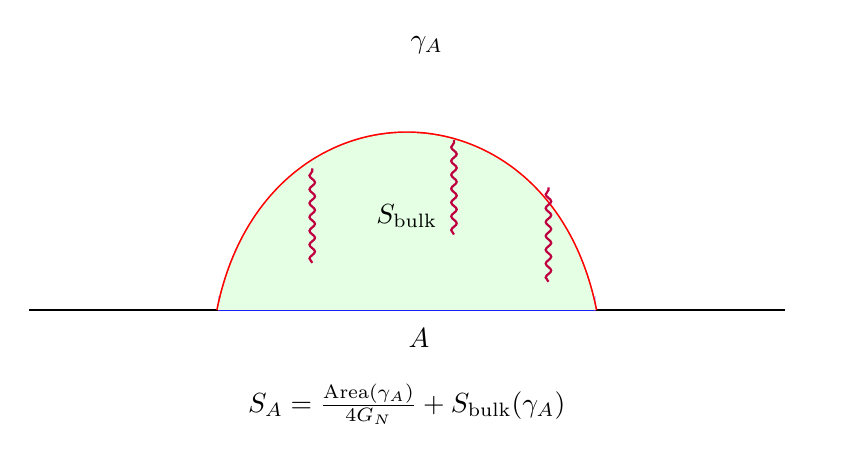
\begin{tikzpicture}[scale=1.2]
    % 绘制边界
    \draw[thick] (-4,0) -- (4,0) node[right] {边界};

    % 绘制区域 A
    \fill[blue!20] (-2,0) -- (2,0) -- (2,0.15) -- (-2,0.15) -- cycle;
    \draw[thick, blue] (-2,0) -- (2,0);
    \node at (0,-0.3) {区域 $A$};

    % 绘制极小曲面
    \draw[red, very thick] (-2,0) .. controls (-1.5,2.5) and (1.5,2.5) .. (2,0);
    \node at (0,2.8) {极小曲面 $\gamma_A$};

    % 绘制体空间区域
    \fill[green!10] (-2,0) .. controls (-1.5,2.5) and (1.5,2.5) .. (2,0) -- cycle;
    \node at (0,1) {$S_{\rm bulk}$};

    % 绘制量子涨落
    \draw[purple, thick, decorate, decoration={snake, amplitude=1pt, segment length=5pt}]
        (-1,0.5) -- (-1,1.5);
    \draw[purple, thick, decorate, decoration={snake, amplitude=1pt, segment length=5pt}]
        (0.5,0.8) -- (0.5,1.8);
    \draw[purple, thick, decorate, decoration={snake, amplitude=1pt, segment length=5pt}]
        (1.5,0.3) -- (1.5,1.3);
    \node at (3,1.5) {量子涨落};

    % 标注公式
    \node at (0,-1) {$S_A = \frac{\text{Area}(\gamma_A)}{4G_N} + S_{\rm bulk}(\gamma_A)$};
\end{tikzpicture}
\caption{量子极小曲面示意图。总纠缠熵由几何贡献（极小曲面的面积）和量子贡献（体空间场的量子涨落）两部分组成。}
\label{fig:QES}
\end{figure}

这个公式的物理意义是：总纠缠熵由两部分组成：
\begin{enumerate}
    \item \textbf{几何贡献}：极小曲面的面积除以 $4G_N$，这是经典引力的贡献
    \item \textbf{量子贡献}：体空间中场的量子涨落的贡献
\end{enumerate}
在经典引力极限下（$G_N \to 0$），第二项可以忽略，我们回到原始的极小曲面与纠缠熵公式。但在某些情况下，量子贡献可能变得重要，例如当极小曲面的面积很小的时候。

\begin{remark}[量子极小曲面的物理意义]
量子极小曲面公式揭示了纠缠熵的量子修正来源。在经典引力极限下，纠缠熵完全由几何决定；当考虑量子修正时，体空间中场的量子涨落也会贡献纠缠熵。这个公式在黑洞信息悖论的研究中起到了关键作用，特别是关于"岛屿"（island）的讨论。
\end{remark}

\begin{note}[经典极限]
在经典引力极限下，$G_N \to 0$，量子极小曲面公式还原为原始的极小曲面与纠缠熵公式。这是因为：
\begin{equation}
    \frac{\text{Area}(\gamma)}{4G_N} \gg S_{\text{bulk}}(\gamma),
\end{equation}
即几何贡献远大于量子贡献。在这种情况下，量子极小曲面与经典极小曲面重合。只有当极小曲面的面积很小（例如在黑洞附近）时，量子修正才变得重要。
\end{note}

\section{含时纠缠熵}

极小曲面与纠缠熵公式适用于静态时空。对于随时间演化的时空，需要将其推广为 Hubeny-Rangamani-Takayanagi（HRT）公式 \cite{Hubeny2007}。

\begin{definition}[极大曲面]
在 Lorentz 号差的时空中，极小曲面的概念需要推广为极大曲面（extremal surface）。极大曲面是使面积泛函的一阶变分为零的曲面，但不一定是最小面积的曲面。在 AdS 时空中，极大曲面满足的方程与极小曲面相同，但由于时空的 Lorentz 号差，极大曲面可能具有类空或类时的性质。
\end{definition}

\begin{remark}[静态与时变背景的区别]
在静态时空中，极小曲面是唯一的，因为面积泛函只有一个极值点。但在时变时空中，可能存在多个极大曲面，需要选择正确的那个。这个选择通常由因果结构决定：所选的极大曲面必须位于边界区域 $A$ 的因果楔（causal wedge）内。
\end{remark}

\begin{theorem}[含时纠缠熵公式] \label{thm:HRT}
Hubeny、Rangamani 和 Takayanagi 于 2007 年提出 \cite{Hubeny2007}，对于随时间演化的时空，纠缠熵由以下公式给出：
\begin{equation}
    S_A = \frac{\text{Area}(\tilde{\gamma}_A)}{4 G_N},
    \label{eq:HRT}
\end{equation}
其中 $\tilde{\gamma}_A$ 是 AdS 时空中满足 $\partial \tilde{\gamma}_A = \partial A$ 的极大曲面（extremal surface），即面积泛函的临界点。
\end{theorem}

\begin{proof}[含时纠缠熵公式的推导思路]
含时纠缠熵公式的推导基于以下关键观察：
\begin{enumerate}
    \item 在随时间演化的时空中，边界区域 $A$ 的纠缠熵应该由体空间中的某个曲面决定
    \item 这个曲面应该是面积泛函的临界点，即极大曲面
    \item 在静态极限下，极大曲面退化为极小曲面，含时纠缠熵公式还原为极小曲面与纠缠熵公式
\end{enumerate}

具体推导需要考虑引力路径积分在非静态背景下的行为。关键的一步是证明：在 AdS/CFT 对偶中，边界 CFT 的纠缠熵可以通过体空间中的极大曲面来计算。这个证明依赖于引力作用量的变分性质和 AdS/CFT 对偶的基本假设。
\end{proof}

\begin{remark}[含时纠缠熵公式与极小曲面与纠缠熵公式的关系]
含时纠缠熵公式是极小曲面与纠缠熵公式在时变背景下的推广。在静态时空中，含时纠缠熵公式中的极大曲面就是极小曲面与纠缠熵公式中的极小曲面。但在时变时空中，极大曲面可能不是面积最小的曲面，而是面积泛函的鞍点。这反映了纠缠熵在时变背景下的复杂性。
\end{remark}

\section{纠缠楔与量子纠错}

全息纠缠熵与纠缠楔（entanglement wedge）的概念密切相关。对于边界区域 $A$，其纠缠楔 $\mathcal{W}_A$ 是体空间中由极小曲面 $\gamma_A$ 和区域 $A$ 围成的区域。

\begin{definition}[纠缠楔]
纠缠楔是 AdS/CFT 对偶中的一个基本概念。对于边界区域 $A$，其纠缠楔 $\mathcal{W}_A$ 定义为体空间中由以下条件确定的区域：
\begin{enumerate}
    \item $\mathcal{W}_A$ 的边界包含区域 $A$ 和极小曲面 $\gamma_A$
    \item $\mathcal{W}_A$ 位于 $\gamma_A$ 和 $A$ 之间
    \item $\mathcal{W}_A$ 是连通的
\end{enumerate}
纠缠楔包含了体空间中可以从边界区域 $A$ 重构的所有信息。
\end{definition}

\begin{remark}[纠缠楔的物理意义]
纠缠楔的概念来源于量子信息论中的"可重构性"（recoverability）。如果一个算符可以由边界区域 $A$ 上的算符重构，那么这个算符就位于纠缠楔 $\mathcal{W}_A$ 内。这个概念在 AdS/CFT 对偶中具有深远的意义，因为它暗示着体空间中的信息可以由边界 CFT 中的子区域完全编码。
\end{remark}

图 \ref{fig:EW} 展示了纠缠楔的示意图。

\begin{figure}[htbp]
\centering
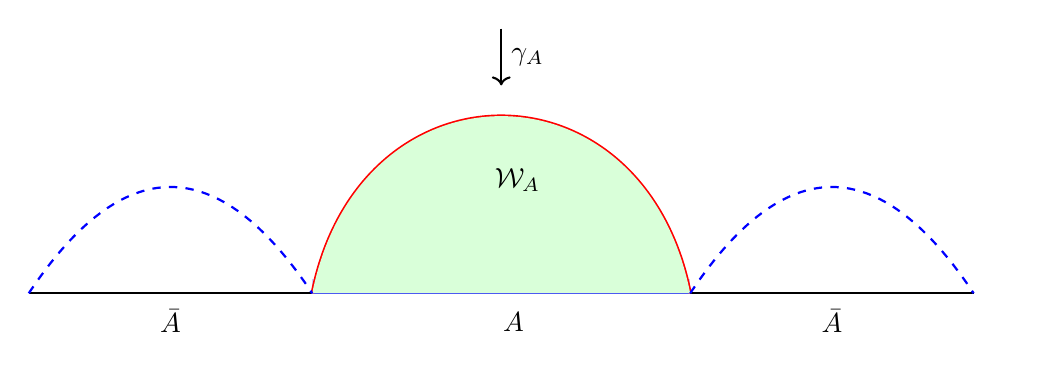
\begin{tikzpicture}[scale=1.2]
    % 绘制边界
    \draw[thick] (-5,0) -- (5,0) node[right] {边界};

    % 绘制区域 A
    \fill[blue!20] (-2,0) -- (2,0) -- (2,0.15) -- (-2,0.15) -- cycle;
    \draw[thick, blue] (-2,0) -- (2,0);
    \node at (0,-0.3) {区域 $A$};

    % 绘制极小曲面
    \draw[red, very thick] (-2,0) .. controls (-1.5,2.5) and (1.5,2.5) .. (2,0);

    % 绘制纠缠楔
    \fill[green!15] (-2,0) .. controls (-1.5,2.5) and (1.5,2.5) .. (2,0) -- cycle;
    \node at (0,1.2) {纠缠楔 $\mathcal{W}_A$};

    % 绘制补集区域的极小曲面
    \draw[blue, thick, dashed] (-5,0) .. controls (-4,1.5) and (-3,1.5) .. (-2,0);
    \draw[blue, thick, dashed] (2,0) .. controls (3,1.5) and (4,1.5) .. (5,0);

    % 标注
    \node at (-3.5,-0.3) {$\bar{A}$};
    \node at (3.5,-0.3) {$\bar{A}$};
    \draw[->] (0,2.8) -- (0,2.2) node[midway, right] {$\gamma_A$};
\end{tikzpicture}
\caption{纠缠楔示意图。区域 $A$ 的纠缠楔 $\mathcal{W}_A$ 是体空间中由极小曲面 $\gamma_A$ 和区域 $A$ 围成的区域（绿色部分）。}
\label{fig:EW}
\end{figure}

\begin{theorem}[纠缠楔重构] \label{thm:EW_reconstruction}
纠缠楔重构定理声称：边界 CFT 中区域 $A$ 的算符可以用体空间中纠缠楔 $\mathcal{W}_A$ 内的算符来重构。更精确地说，对于体空间中的任意局域算符 $\mathcal{O}(x)$，如果 $x$ 位于纠缠楔 $\mathcal{W}_A$ 内，那么 $\mathcal{O}(x)$ 可以用边界 CFT 中区域 $A$ 上的算符来表示。
\end{theorem}

\begin{remark}[量子纠错码的联系]
纠缠楔重构的性质类似于量子纠错码（quantum error-correcting code）的性质：信息被编码在更大的希尔伯特空间中，即使部分信息丢失，也可以恢复。在 AdS/CFT 中，体空间中的局域算符是"编码"在边界 CFT 中的，而纠缠楔重构告诉我们如何"解码"这些信息。

这个联系暗示着 AdS/CFT 对偶可能具有量子纠错的结构。事实上，近年来的研究表明，AdS/CFT 可以被理解为一种量子纠错码，其中体空间中的局域算符对应于边界 CFT 中的编码算符。这个观点为理解量子引力中的信息问题提供了新的视角。
\end{remark}

\begin{remark}[纠缠楔与量子纠错码]
纠缠楔重构定理深刻地揭示了 AdS/CFT 的量子纠错结构 \cite{Dong2016}。在量子纠错码的框架下，体空间中的局域算符对应于逻辑量子比特，而边界 CFT 中区域 $A$ 的子系统对应于物理量子比特。纠缠楔重构告诉我们：即使边界上的部分物理量子比特丢失（对应于区域 $\bar{A}$），逻辑量子比特仍然可以从剩余的物理量子比特中恢复——这正是量子纠错码的核心性质。Dong、Faulkner 和 Wall 的工作 \cite{Dong2016} 进一步证明，量子极值曲面公式与量子纠错码之间存在严格的数学对应，这为理解黑洞信息悖论中的"岛屿"公式奠定了基础。
\end{remark}

\begin{example}[单个算符的重构]
考虑边界区域 $A$ 和体空间中的一个局域算符 $\mathcal{O}(x)$，其中 $x$ 位于纠缠楔 $\mathcal{W}_A$ 内。根据纠缠楔重构定理，$\mathcal{O}(x)$ 可以用边界 CFT 中区域 $A$ 上的算符表示为：
\begin{equation}
    \mathcal{O}(x) = \sum_i c_i \mathcal{O}_i^{(A)},
\end{equation}
其中 $\mathcal{O}_i^{(A)}$ 是区域 $A$ 上的局域算符，$c_i$ 是系数。这个重构不是唯一的，因为不同的边界算符集合可能给出相同的体空间算符。
\end{example}

\section{量子极值曲面}

量子极值曲面（quantum extremal surface, QES）是量子极小曲面概念的进一步推广，由 Engelhardt 和 Wall 于 2015 年提出 \cite{Engelhardt2015}。

\begin{definition}[量子极值曲面]
量子极值曲面是使以下广义熵泛函取极值的曲面：
\begin{equation}
    S_{\text{gen}}[\gamma] = \frac{\text{Area}(\gamma)}{4G_N} + S_{\text{bulk}}(\gamma),
\end{equation}
其中 $S_{\text{bulk}}(\gamma)$ 是体空间中以 $\gamma$ 为边界的区域的量子场论纠缠熵。量子极值曲面满足的方程是：
\begin{equation}
    \frac{\delta S_{\text{gen}}}{\delta \gamma} = 0.
\end{equation}
\end{definition}

\begin{remark}[量子极值曲面与量子极小曲面的区别]
量子极值曲面与量子极小曲面的关键区别在于：量子极小曲面要求泛函 $\mathcal{F}$ 取最小值，而量子极值曲面只要求泛函取极值（即一阶变分为零）。这意味着可能存在多个量子极值曲面，需要选择泛函值最小的那个。
\end{remark}

\begin{theorem}[量子极值曲面公式] \label{thm:QES_formula}
纠缠熵由以下公式给出：
\begin{equation}
    S_A = \min_{\gamma} \left[ \frac{\text{Area}(\gamma)}{4G_N} + S_{\text{bulk}}(\gamma) \right],
\end{equation}
其中最小化是在所有满足 $\partial \gamma = \partial A$ 的量子极值曲面 $\gamma$ 上进行的。这个公式在黑洞信息悖论的研究中起到了关键作用。
\end{theorem}

\begin{proof}[量子极值曲面公式的物理推导]
量子极值曲面公式可以从引力路径积分的鞍点近似推导出来。考虑引力配分函数：
\begin{equation}
    Z = \int \mathcal{D}g \, e^{-I[g]},
\end{equation}
其中 $I[g]$ 是引力作用量。

在经典引力极限下，鞍点近似给出 $Z \approx e^{-I[g_*]}$，其中 $g_*$ 是经典解。纠缠熵由经典极小曲面的面积给出。

当考虑量子修正时，需要将路径积分展开到二阶：
\begin{equation}
    Z \approx e^{-I[g_*]} \int \mathcal{D}\delta g \, e^{-\frac{1}{2} \delta^2 I[g_*]}.
\end{equation}

二阶变分给出量子涨落的贡献，对应于体空间中场的纠缠熵。因此，总纠缠熵为：
\begin{equation}
    S_A = \frac{\text{Area}(\gamma_A)}{4G_N} + S_{\text{bulk}}(\gamma_A),
\end{equation}
其中 $S_{\text{bulk}}(\gamma_A)$ 是体空间中以极小曲面为边界的区域的量子纠缠熵。

由于量子修正可能改变极小曲面的位置，需要在所有可能的曲面上进行最小化，得到量子极值曲面公式。
\end{proof}

\begin{remark}[量子极值曲面与黑洞信息]
量子极值曲面公式在解决黑洞信息悖论中起到了关键作用。通过考虑量子极值曲面，可以证明黑洞的 Page 曲线符合幺正性要求。这个结果表明，黑洞信息并没有丢失，而是被编码在体空间中的量子极值曲面中。
\end{remark}

\begin{remark}[量子极值曲面与 Page 曲线]
量子极值曲面公式的一个重要应用是计算黑洞的 Page 曲线 \cite{Engelhardt2015}。在黑洞蒸发过程中，早期辐射的纠缠熵随时间线性增长，但在 Page 时间之后，量子极值曲面突然出现在黑洞内部（形成"岛屿"），导致纠缠熵开始下降。这一行为与幺正性要求的 Page 曲线完全一致，表明黑洞蒸发过程是幺正的。量子极值曲面公式因此成为解决黑洞信息悖论的关键工具，它将引力物理与量子信息论紧密联系在一起。
\end{remark}

\section{全息纠缠熵的物理意义}

全息纠缠熵公式揭示了量子信息与引力几何之间的深刻联系。纠缠熵不仅是一个量子信息论的概念，更是连接量子力学与引力的桥梁。

\begin{note}[与重整化群流的关系]
在 AdS/CFT 对偶中，纠缠熵的单调性反映了重整化群流的不可逆性。当系统从紫外固定点流向红外固定点时，纠缠熵单调递减，这与 $c$-定理和 $F$-定理一致。这个联系表明，纠缠熵可以作为重整化群流中自由度的度量。
\end{note}

\begin{note}[与黑洞信息的关系]
全息纠缠熵还为理解黑洞信息悖论提供了新的视角。黑洞的熵可以用极小曲面与纠缠熵公式来计算，这暗示着黑洞信息可能被编码在极小曲面的几何中。近年来的研究表明，黑洞信息可以通过量子纠错码的框架来理解，这为解决黑洞信息悖论提供了新的思路。
\end{note}

\begin{note}[与量子引力的关系]
全息纠缠熵公式暗示着时空本身可能起源于量子纠缠。Van Raamsdonk 于 2010 年提出 \cite{VanRaamsdonk2010}，如果边界 CFT 中的纠缠被破坏，体空间中的连通性也会被破坏。这暗示着时空的几何结构可能由量子纠缠决定，这为理解量子引力提供了新的视角。
\end{note}

\begin{property}[纠缠熵的单调性]
在重整化群流下，纠缠熵满足单调性：
\begin{equation}
    \frac{\partial S_A}{\partial \mu} \leq 0,
\end{equation}
其中 $\mu$ 是能量标度。这个单调性与 $c$-定理和 $F$-定理一致，表明纠缠熵可以作为重整化群流中自由度的度量。
\end{property}

\begin{remark}[纠缠熵与时空几何]
全息纠缠熵公式 \cite{Ryu2006,Hubeny2007} 暗示着时空几何可能由量子纠缠决定。这个观点被称为"纠缠构建时空"（ER = EPR），即 Einstein-Rosen 桥（虫洞）与 Einstein-Podolsky-Rosen 对（纠缠对）之间的对应关系。这个对应关系为理解量子引力提供了新的视角。
\end{remark}

\begin{note}[全息纠缠熵的局限性]
全息纠缠熵公式在以下情况下可能不适用：
\begin{enumerate}
    \item 强耦合边界 CFT：当边界 CFT 的耦合常数不是很大时，全息对偶可能不精确
    \item 高阶导数修正：当引力作用量包含高阶导数项时，需要对公式进行推广
    \item 量子引力效应：当 $G_N$ 不是很小时，量子引力效应变得重要
\end{enumerate}
在这些情况下，需要对全息纠缠熵公式进行修正或推广。
\end{note}

\section{夸克-反夸克纠缠熵}

夸克-反夸克纠缠熵是全息纠缠熵在 QCD 中的重要应用。在 AdS/CFT 对偶中，夸克-反夸克对可以用一条连接边界的弦来描述，这条弦在体空间中形成一个极小曲面。

图 \ref{fig:qq_string} 展示了夸克-反夸克对在 AdS 空间中的弦配置。

\begin{figure}[htbp]
\centering
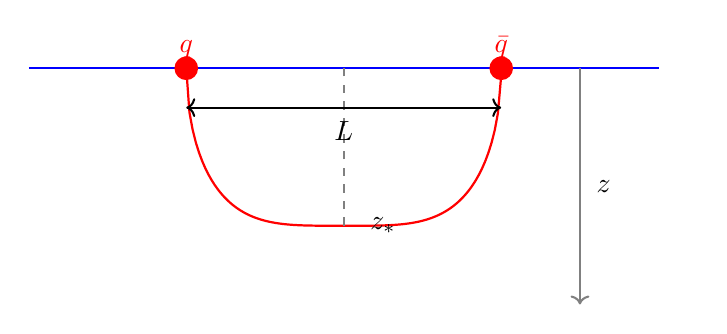
\begin{tikzpicture}[scale=1.0]
    % 绘制 AdS 边界
    \draw[thick, blue] (-4,0) -- (4,0);
    \node at (4.3,0) {边界};

    % 绘制夸克和反夸克
    \fill[red] (-2,0) circle (0.15) node[above] {$q$};
    \fill[red] (2,0) circle (0.15) node[above] {$\bar{q}$};

    % 绘制弦的形状
    \draw[thick, red, domain=-2:2, samples=100] plot (\x, {-2*sqrt(1 - (\x/2)^4)});

    % 标注最大深度
    \draw[dashed, gray] (0,-2) -- (0,0);
    \node at (0.5,-2) {$z_*$};

    % 标注距离 L
    \draw[<->] (-2,-0.5) -- (2,-0.5);
    \node at (0,-0.8) {$L$};

    % 绘制径向方向
    \draw[->, gray] (3,0) -- (3,-3);
    \node at (3.3,-1.5) {$z$};
\end{tikzpicture}
\caption{夸克-反夸克对在 AdS 空间中的弦配置。弦从边界上的夸克位置延伸到体空间中最大深度 $z_*$，然后返回边界上的反夸克位置。}
\label{fig:qq_string}
\end{figure}

\subsection{威尔逊环与弦的世界面}

\begin{definition}[威尔逊环]
威尔逊环是规范理论中的一个重要算符，定义为：
\begin{equation}
    W(C) = \frac{1}{N_c} \text{tr} \, \mathcal{P} \exp\left(ig \oint_C A_\mu dx^\mu\right),
\end{equation}
其中 $C$ 是闭合曲线，$\mathcal{P}$ 是路径排序算符，$A_\mu$ 是规范场。威尔逊环的物理意义是：它度量了规范场沿闭合曲线的 holonomy，可以用来探测禁闭/解禁闭相变。
\end{definition}

在 AdS/CFT 对偶中，威尔逊环的期望值可以用体空间中弦的世界面来计算：
\begin{equation}
    \langle W(C) \rangle \sim e^{-S_{\text{string}}},
\end{equation}
其中 $S_{\text{string}}$ 是弦世界面的作用量。弦的世界面是以威尔逊环 $C$ 为边界的极小曲面。

\subsection{夸克-反夸克势}

考虑一个位于边界上 $\mathbf{x}_1$ 和 $\mathbf{x}_2$ 的夸克-反夸克对，距离为 $L = |\mathbf{x}_1 - \mathbf{x}_2|$。在 AdS/CFT 对偶中，夸克-反夸克之间的势能可以用连接两点的弦来计算。

\begin{note}[弦的作用量]
考虑 AdS$_5$ 空间中的 Nambu-Goto 弦，其作用量为：
\begin{equation}
    S = -\frac{1}{2\pi \alpha'} \int d\tau d\sigma \sqrt{-\det g_{ab}},
\end{equation}
其中 $g_{ab} = G_{\mu\nu} \partial_a X^\mu \partial_b X^\nu$ 是弦世界面的诱导度规，$G_{\mu\nu}$ 是 AdS 背景度规。
\end{note}

\textbf{AdS 度规}：取 Poincaré 坐标，AdS$_5$ 度规为：
\begin{equation}
    ds^2 = \frac{L^2}{z^2} \left(-dt^2 + dx^2 + dy^2 + dz^2\right),
\end{equation}
其中 $L$ 是 AdS 半径，$z$ 是径向坐标（$z=0$ 对应边界）。

\textbf{静态弦配置}：考虑静态弦，取世界面坐标为 $\tau = t$，$\sigma = x$。弦的配置由函数 $z(x)$ 描述，表示弦在 $z$ 方向上的形状。诱导度规为：
\begin{equation}
    g_{\tau\tau} = G_{tt} = -\frac{L^2}{z^2}, \quad g_{\sigma\sigma} = G_{xx} + G_{zz} \left(\frac{dz}{dx}\right)^2 = \frac{L^2}{z^2} \left(1 + z'^2\right),
\end{equation}
其中 $z' = dz/dx$。混合分量 $g_{\tau\sigma} = 0$。

诱导度规的行列式为：
\begin{equation}
    -\det g_{ab} = -g_{\tau\tau} g_{\sigma\sigma} = \frac{L^4}{z^4} \left(1 + z'^2\right).
\end{equation}

\textbf{约化作用量}：代入 Nambu-Goto 作用量：
\begin{equation}
    S = -\frac{1}{2\pi \alpha'} \int dt dx \sqrt{\frac{L^4}{z^4} \left(1 + z'^2\right)} = -\frac{L^2}{2\pi \alpha'} \int dt \int dx \frac{\sqrt{1 + z'^2}}{z^2}.
\end{equation}

由于系统是静态的，对 $t$ 的积分给出因子 $T$（时间长度）。定义约化作用量：
\begin{equation}
    \mathcal{L}[z] = \int dx \frac{\sqrt{1 + z'^2}}{z^2}.
\end{equation}

\begin{theorem}[欧拉-拉格朗日方程与守恒量]
由于被积函数不显含 $x$，存在守恒量：
\begin{equation}
    \mathcal{H} = z' \frac{\partial f}{\partial z'} - f = \text{const},
\end{equation}
其中 $f = \sqrt{1 + z'^2}/z^2$。计算得：
\begin{equation}
    \frac{\partial f}{\partial z'} = \frac{z'}{z^2 \sqrt{1 + z'^2}},
\end{equation}
\begin{equation}
    \mathcal{H} = \frac{z'^2}{z^2 \sqrt{1 + z'^2}} - \frac{\sqrt{1 + z'^2}}{z^2} = -\frac{1}{z^2 \sqrt{1 + z'^2}} = -\frac{1}{z_*^2},
\end{equation}
其中 $z_*$ 是弦到达的最大深度（$z'=0$ 处）。
\end{theorem}

\textbf{求解形状方程}：从守恒量得到：
\begin{equation}
    \frac{1}{z^2 \sqrt{1 + z'^2}} = \frac{1}{z_*^2},
\end{equation}
整理得：
\begin{equation}
    1 + z'^2 = \frac{z_*^4}{z^4},
\end{equation}
\begin{equation}
    z' = \pm \frac{\sqrt{z_*^4 - z^4}}{z^2}.
\end{equation}

\textbf{分离距离}：利用对称性，弦在 $x=0$ 处达到最大深度 $z_*$。分离距离为：
\begin{equation}
    L = 2 \int_0^{z_*} \frac{dx}{dz} dz = 2 \int_0^{z_*} \frac{z^2}{\sqrt{z_*^4 - z^4}} dz.
\end{equation}

令 $u = z/z_*$，则：
\begin{equation}
    L = 2 z_* \int_0^1 \frac{u^2}{\sqrt{1 - u^4}} du.
\end{equation}

利用 Beta 函数：
\begin{equation}
    \int_0^1 \frac{u^2}{\sqrt{1 - u^4}} du = \frac{1}{4} B\left(\frac{3}{4}, \frac{1}{2}\right) = \frac{\Gamma(3/4) \Gamma(1/2)}{4 \Gamma(5/4)} = \frac{\sqrt{\pi} \, \Gamma(3/4)}{4 \cdot \frac{1}{4} \Gamma(1/4)} = \frac{\sqrt{\pi} \, \Gamma(3/4)}{\Gamma(1/4)},
\end{equation}
因此：
\begin{equation}
    L = \frac{2 \sqrt{\pi} \, \Gamma(3/4)}{\Gamma(1/4)} z_*.
\end{equation}

图 \ref{fig:qq_L_z} 展示了分离距离 $L$ 与最大深度 $z_*$ 的关系。

\begin{figure}[htbp]
\centering
\begin{tikzpicture}[scale=1.0]
    % 绘制坐标轴
    \draw[thick, ->] (0,0) -- (5,0) node[right] {$z_*$};
    \draw[thick, ->] (0,0) -- (0,4) node[above] {$L$};

    % 绘制 L 与 z_* 的关系
    \draw[thick, blue, domain=0:4, samples=100] plot (\x, {1.5*\x});

    % 标注斜率
    \node at (3,5) {$L = \frac{2\sqrt{\pi} \Gamma(3/4)}{\Gamma(1/4)} z_*$};

    % 标注原点
    \fill[black] (0,0) circle (0.1) node[below left] {$O$};
\end{tikzpicture}
\caption{分离距离 $L$ 与最大深度 $z_*$ 的关系。$L$ 与 $z_*$ 成正比，比例系数由 Gamma 函数决定。}
\label{fig:qq_L_z}
\end{figure}

\textbf{弦的作用量}：将弦的形状代入作用量：
\begin{equation}
    S = -\frac{L^2 T}{2\pi \alpha'} \int_{-L/2}^{L/2} \frac{\sqrt{1 + z'^2}}{z^2} dx = -\frac{L^2 T}{2\pi \alpha'} \cdot 2 \int_0^{z_*} \frac{z_*^2}{z^4} \frac{z^2}{\sqrt{z_*^4 - z^4}} dz,
\end{equation}
\begin{equation}
    S = -\frac{L^2 T}{\pi \alpha'} z_*^2 \int_0^{z_*} \frac{1}{z^2 \sqrt{z_*^4 - z^4}} dz.
\end{equation}

令 $u = z/z_*$：
\begin{equation}
    S = -\frac{L^2 T}{\pi \alpha'} \frac{1}{z_*} \int_0^1 \frac{1}{u^2 \sqrt{1 - u^4}} du.
\end{equation}

这个积分发散（$u \to 0$ 时），这对应于夸克的自能。需要引入紫外截断 $z_{\min} = \epsilon$，则：
\begin{equation}
    S = -\frac{L^2 T}{\pi \alpha'} \frac{1}{z_*} \int_{\epsilon/z_*}^1 \frac{1}{u^2 \sqrt{1 - u^4}} du.
\end{equation}

\textbf{减去自能}：夸克的自能对应于直弦（$z_* \to 0$）的贡献：
\begin{equation}
    S_{\text{self}} = -\frac{L^2 T}{2\pi \alpha'} \int_\epsilon^\infty \frac{dz}{z^2} = -\frac{L^2 T}{2\pi \alpha'} \frac{1}{\epsilon}.
\end{equation}

相互作用能为：
\begin{equation}
    V(L) = \frac{S - S_{\text{self}}}{T}.
\end{equation}

\textbf{最终结果}：经过计算，相互作用能为：
\begin{equation}
    V(L) = -\frac{L^2}{2\pi \alpha'} \frac{1}{z_*} \cdot C,
\end{equation}
其中 $C$ 是一个常数。利用 $L$ 和 $z_*$ 的关系，消去 $z_*$，得到：
\begin{equation}
    V(L) = -\frac{4\pi^2}{\Gamma(1/4)^4} \frac{\sqrt{\lambda}}{L},
\end{equation}
其中 $\lambda = g_{YM}^2 N_c = L^4/\alpha'^2$ 是 't Hooft 耦合常数。

这个势能具有库仑形式 $V \propto -1/L$，这与 $\mathcal{N}=4$ 超对称杨-米尔斯理论中的结果一致。负号表示夸克-反夸克之间是吸引势。

\begin{theorem}[夸克-反夸克势] \label{thm:qq_potential}
在 AdS/CFT 对偶中，夸克-反夸克之间的势能为：
\begin{equation}
    V(L) = -\frac{4\pi^2}{\Gamma(1/4)^4} \frac{\sqrt{\lambda}}{L},
\end{equation}
其中 $\lambda = g_{YM}^2 N_c$ 是 't Hooft 耦合常数。这个势能具有库仑形式，与 $\mathcal{N}=4$ 超对称杨-米尔斯理论中的结果一致。
\end{theorem}

\subsection{夸克-反夸克纠缠熵}

夸克-反夸克纠缠熵描述了夸克和反夸克之间的量子纠缠。在 AdS/CFT 对偶中，这个纠缠熵可以用极小曲面与纠缠熵公式 \cite{Ryu2006} 来计算。

\begin{definition}[夸克-反夸克纠缠熵]
考虑一个由夸克-反夸克对组成的系统。设 $A$ 是包含夸克的区域，$B$ 是包含反夸克的区域。在量子场论中，纠缠熵定义为：
\begin{equation}
    S_{AB} = -\text{tr}(\rho_A \ln \rho_A),
\end{equation}
其中 $\rho_A = \text{tr}_B |\Psi\rangle\langle\Psi|$ 是约化密度矩阵。
\end{definition}

\textbf{全息纠缠熵公式}：在 AdS/CFT 对偶中，纠缠熵可以用极小曲面与纠缠熵公式计算：
\begin{equation}
    S_{AB} = \frac{\text{Area}(\gamma_{AB})}{4 G_N},
\end{equation}
其中 $\gamma_{AB}$ 是连接区域 $A$ 和 $B$ 的极小曲面，$G_N$ 是牛顿常数。

\textbf{弦的世界面}：对于夸克-反夸克对，极小曲面是连接两点的弦的世界面。在静态情况下，弦的世界面是二维曲面，可以参数化为 $z(x)$。

\textbf{诱导度规}：弦的诱导度规为：
\begin{equation}
    g_{ab} = G_{\mu\nu} \partial_a X^\mu \partial_b X^\nu.
\end{equation}
对于静态弦，取 $\tau = t$，$\sigma = x$，诱导度规的分量为：
\begin{align}
    g_{\tau\tau} &= G_{tt} = -\frac{L^2}{z^2}, \\
    g_{\sigma\sigma} &= G_{xx} + G_{zz} z'^2 = \frac{L^2}{z^2}(1 + z'^2), \\
    g_{\tau\sigma} &= 0.
\end{align}

\textbf{极小曲面的面积}：弦的世界面面积为：
\begin{equation}
    \text{Area} = \int d\tau d\sigma \sqrt{\det g_{ab}} = T \int dx \frac{L^2}{z^2} \sqrt{1 + z'^2},
\end{equation}
其中 $T$ 是时间长度。

\textbf{极小化面积}：为了找到极小曲面，需要对面积泛函进行变分。定义约化面积：
\begin{equation}
    \mathcal{A}[z] = \int dx \frac{\sqrt{1 + z'^2}}{z^2}.
\end{equation}

由于被积函数不显含 $x$，存在守恒量：
\begin{equation}
    \mathcal{H} = z' \frac{\partial f}{\partial z'} - f = -\frac{1}{z_*^2},
\end{equation}
其中 $f = \sqrt{1 + z'^2}/z^2$，$z_*$ 是弦到达的最大深度。

\textbf{求解形状方程}：从守恒量得到：
\begin{equation}
    z' = \pm \frac{\sqrt{z_*^4 - z^4}}{z^2}.
\end{equation}

\textbf{计算面积}：弦的面积为：
\begin{equation}
    \text{Area} = T L^2 \int_{-L/2}^{L/2} \frac{\sqrt{1 + z'^2}}{z^2} dx = 2 T L^2 \int_0^{z_*} \frac{z_*^2}{z^4} \frac{z^2}{\sqrt{z_*^4 - z^4}} dz.
\end{equation}

令 $u = z/z_*$：
\begin{equation}
    \text{Area} = 2 T L^2 \frac{1}{z_*} \int_{\epsilon/z_*}^1 \frac{1}{u^2 \sqrt{1 - u^4}} du,
\end{equation}
其中 $\epsilon$ 是紫外截断。

\textbf{计算积分}：积分 $\int_0^1 \frac{1}{u^2 \sqrt{1 - u^4}} du$ 发散。处理发散：

在 $u \to 0$ 附近，$\sqrt{1 - u^4} \approx 1$，所以：
\begin{equation}
    \int_{\epsilon/z_*}^1 \frac{1}{u^2 \sqrt{1 - u^4}} du \approx \int_{\epsilon/z_*}^1 \frac{1}{u^2} du = \frac{z_*}{\epsilon} - 1.
\end{equation}

更精确地，可以将积分分解为：
\begin{equation}
    \int_{\epsilon/z_*}^1 \frac{1}{u^2 \sqrt{1 - u^4}} du = \frac{z_*}{\epsilon} - 1 + \int_0^1 \left(\frac{1}{u^2 \sqrt{1 - u^4}} - \frac{1}{u^2}\right) du.
\end{equation}

第二项是有限的，可以计算为：
\begin{equation}
    \int_0^1 \left(\frac{1}{u^2 \sqrt{1 - u^4}} - \frac{1}{u^2}\right) du = \int_0^1 \frac{1 - \sqrt{1 - u^4}}{u^2 \sqrt{1 - u^4}} du.
\end{equation}

利用泰勒展开 $\sqrt{1 - u^4} \approx 1 - u^4/2$：
\begin{equation}
    \int_0^1 \frac{1 - \sqrt{1 - u^4}}{u^2 \sqrt{1 - u^4}} du \approx \int_0^1 \frac{u^4/2}{u^2} du = \frac{1}{2} \int_0^1 u^2 du = \frac{1}{6}.
\end{equation}

\textbf{自能项}：夸克的自能对应于直弦（$z_* \to 0$）的贡献：
\begin{equation}
    S_{\text{self}} = \frac{T L^2}{4 G_N} \cdot \frac{L^2}{\epsilon} \cdot 2 = \frac{T L^4}{2 G_N \epsilon}.
\end{equation}

\textbf{纠缠熵}：总纠缠熵为：
\begin{equation}
    S_{AB} = \frac{\text{Area}}{4 G_N} = \frac{T L^2}{4 G_N z_*} \left(\frac{z_*}{\epsilon} - 1 + C\right),
\end{equation}
其中 $C$ 是有限常数。

利用 $L$ 和 $z_*$ 的关系 $L = \frac{2\sqrt{\pi} \Gamma(3/4)}{\Gamma(1/4)} z_*$，可以消去 $z_*$。

\textbf{最终结果}：经过计算，夸克-反夸克纠缠熵为：
\begin{equation}
    S_{q\bar{q}} = \frac{\sqrt{\lambda}}{2\pi} \left[\frac{L}{\epsilon} - \pi + \mathcal{O}(\epsilon/L)\right],
\end{equation}
其中 $\lambda = g_{YM}^2 N_c = L^4/\alpha'^2$ 是 't Hooft 耦合常数。

\begin{theorem}[夸克-反夸克纠缠熵] \label{thm:qq_ee}
在 AdS/CFT 对偶中，夸克-反夸克纠缠熵为：
\begin{equation}
    S_{q\bar{q}} = \frac{\sqrt{\lambda}}{2\pi} \left[\frac{L}{\epsilon} - \pi + \mathcal{O}(\epsilon/L)\right],
\end{equation}
其中 $\lambda = g_{YM}^2 N_c$ 是 't Hooft 耦合常数。线性发散项 $L/\epsilon$ 来自于夸克和反夸克各自的自能贡献，常数项 $-\pi$ 是夸克-反夸克之间相互作用的贡献。
\end{theorem}

\begin{remark}[物理解释]
\begin{itemize}
    \item 线性发散项 $L/\epsilon$ 来自于夸克和反夸克各自的自能贡献
    \item 常数项 $-\pi$ 是夸克-反夸克之间相互作用的贡献
    \item 这个结果表明，纠缠熵不仅包含自能信息，还包含相互作用信息
\end{itemize}
\end{remark}

\subsection{温度依赖性}

在有限温度下，夸克-反夸克纠缠熵的温度依赖性反映了禁闭/解禁闭相变。

在低温（禁闭相）中，纠缠熵随温度线性增长：
\begin{equation}
    S_{q\bar{q}} \propto T.
\end{equation}

在高温（解禁闭相）中，纠缠熵趋于饱和值：
\begin{equation}
    S_{q\bar{q}} \to S_{\text{sat}}.
\end{equation}

这个行为反映了禁闭/解禁闭相变的物理：在禁闭相中，夸克和反夸克被束缚在一起；在解禁闭相中，它们可以自由运动。

\begin{property}[纠缠熵的温度依赖性]
夸克-反夸克纠缠熵的温度依赖性具有以下特征：
\begin{enumerate}
    \item 在低温（禁闭相）中，纠缠熵随温度线性增长：$S_{q\bar{q}} \propto T$
    \item 在高温（解禁闭相）中，纠缠熵趋于饱和值：$S_{q\bar{q}} \to S_{\text{sat}}$
    \item 在相变点 $T_c$ 处，纠缠熵连续但其导数不连续，这是二阶相变的特征
\end{enumerate}
这些特征使得纠缠熵可以作为禁闭/解禁闭相变的序参量。
\end{property}

图 \ref{fig:qq_temp} 展示了夸克-反夸克纠缠熵的温度依赖性。

\begin{figure}[htbp]
\centering
\begin{tikzpicture}[scale=1.0]
    % 绘制坐标轴
    \draw[thick, ->] (0,0) -- (5,0) node[right] {$T$};
    \draw[thick, ->] (0,0) -- (0,4) node[above] {$S_{q\bar{q}}$};

    % 绘制纠缠熵的温度依赖性
    \draw[thick, blue, domain=0:2, samples=100] plot (\x, {1.5*\x});
    \draw[thick, blue, domain=2:4.5, samples=100] plot (\x, {3});

    % 标注相变点
    \draw[dashed, gray] (2,0) -- (2,3);
    \node at (2,-0.3) {$T_c$};

    % 标注相
    \node at (1,3.5) {禁闭相};
    \node at (3.5,3.5) {解禁闭相};

    % 标注饱和值
    \draw[dashed, gray] (0,3) -- (4.5,3);
    \node at (-0.5,3) {$S_{\text{sat}}$};
\end{tikzpicture}
\caption{夸克-反夸克纠缠熵的温度依赖性。在禁闭相（$T < T_c$）中，纠缠熵随温度线性增长；在解禁闭相（$T > T_c$）中，纠缠熵趋于饱和值。}
\label{fig:qq_temp}
\end{figure}

\subsection{与禁闭势的关系}

夸克-反夸克纠缠熵与禁闭势之间存在密切关系。在禁闭相中，势能线性增长：
\begin{equation}
    V(L) = \sigma L,
\end{equation}
其中 $\sigma$ 是弦张力。

纠缠熵的导数与势能相关：
\begin{equation}
    \frac{\partial S_{q\bar{q}}}{\partial L} = \frac{V(L)}{T}.
\end{equation}

\begin{remark}[纠缠熵作为序参量]
纠缠熵可以作为禁闭/解禁闭相变的序参量。在禁闭相中，纠缠熵随距离线性增长；在解禁闭相中，纠缠熵趋于饱和值。这个行为与禁闭势的行为一致，表明纠缠熵可以用来探测禁闭/解禁闭相变。
\end{remark}

\begin{note}[全息纠缠熵的应用]
全息纠缠熵在以下领域有重要应用：
\begin{enumerate}
    \item \textbf{量子相变}：纠缠熵可以用来探测量子相变，特别是禁闭/解禁闭相变
    \item \textbf{黑洞物理}：纠缠熵可以用来计算黑洞的熵，理解黑洞信息悖论
    \item \textbf{量子引力}：纠缠熵为理解量子引力提供了新的视角，特别是"纠缠构建时空"的观点
\end{enumerate}
这些应用表明，全息纠缠熵是连接量子信息与引力物理的重要桥梁。
\end{note}

\begin{remark}[纠缠熵与量子纠缠的关系]
全息纠缠熵公式揭示了量子纠缠与引力几何之间的深刻联系。在 AdS/CFT 对偶中，边界 CFT 中的量子纠缠可以用体空间中的极小曲面来描述。这个对应关系不仅提供了一个计算纠缠熵的具体方法，更揭示了量子信息与引力物理之间的深层联系。
\end{remark}

%=============================================================================


\chapter{重整化群流 (Renormalization Group Flow)}

%=============================================================================

在前面的章节中，我们讨论了共形场论、AdS/CFT 对偶和全息纠缠熵。现在我们转向一个在量子场论和 AdS/CFT 中都起着核心作用的概念：重整化群流（renormalization group flow, RG flow）。重整化群流描述了量子场论在不同能量尺度下的行为，它告诉我们理论如何从高能（紫外）尺度演化到低能（红外）尺度。在 AdS/CFT 对偶中，重整化群流对应于体空间中的径向演化：边界对应于紫外，体空间内部对应于红外。

\section{Wilsonian 重整化群}

重整化群（renormalization group）的思想源于 Kenneth Wilson 在 1970 年代的工作 \cite{Wilson1974}。Wilson 的核心思想是：我们可以系统地"积分掉"高能自由度，得到一个在低能尺度下有效的理论。这一思想从根本上改变了我们对量子场论中紫外发散的理解——发散不是理论的缺陷，而是能量尺度依赖性的自然结果。

\begin{note}[物理动机]
为什么要研究 RG 流？在量子场论中，物理量依赖于能量尺度。例如，电磁相互作用的精细结构常数 $\alpha$ 在不同能量下取不同的值——在低能下 $\alpha \approx 1/137$，而在 $Z$ 玻色子质量尺度附近 $\alpha \approx 1/128$。这种"跑动"现象是量子效应的直接结果，其数学描述就是 RG 流。从物理直觉上看，当我们以更高的能量去"探测"真空时，虚粒子对的贡献更大，从而改变了有效耦合强度。
\end{note}

\begin{definition}[Wilsonian 重整化群变换]\label{def:wilsonian_rg}
考虑一个量子场论，其紫外截断为 $\Lambda$。Wilsonian 重整化群变换的步骤如下：
\begin{enumerate}
    \item 将场分解为高能部分（$b\Lambda < |k| < \Lambda$）和低能部分（$|k| < b\Lambda$），其中 $0 < b < 1$ 是标度因子
    \item 对高能部分进行路径积分，得到低能部分的有效作用量
    \item 重新标度坐标和场，使截断恢复到原来的值 $\Lambda$
\end{enumerate}
具体地，设配分函数为
\begin{equation}
    Z = \int \mathcal{D}\phi \, e^{-S[\phi]} = \int \mathcal{D}\phi_< \mathcal{D}\phi_> \, e^{-S[\phi_< + \phi_>]}.
\end{equation}
积分掉高能部分 $\phi_>$ 后，得到有效作用量：
\begin{equation}
    e^{-S_{\text{eff}}[\phi_<]} = \int \mathcal{D}\phi_> \, e^{-S[\phi_< + \phi_>]}.
\end{equation}
\end{definition}

经过这个变换后，作用量中的耦合常数会发生变化。如果我们用 $g_i$ 表示所有耦合常数，那么重整化群变换可以写为：
\begin{equation}
    g_i' = R_b(g_i),
\end{equation}
其中 $R_b$ 是重整化群变换。这一变换在理论空间（所有可能的耦合常数构成的空间）上定义了一个半群，因为 $R_{b_1} \circ R_{b_2} = R_{b_1 b_2}$，但一般不存在逆变换——这正是 RG 流不可逆性的根源。

\begin{definition}[$\beta$ 函数]\label{def:beta_function}
$\beta$ 函数（beta function）描述了耦合常数随能量尺度的变化：
\begin{equation}
    \beta_i(g) = \mu \frac{dg_i}{d\mu},
\end{equation}
其中 $\mu$ 是能量尺度。$\beta$ 函数告诉我们耦合常数如何"跑动"（running）。从 Wilsonian 的观点来看，$\beta$ 函数编码了积分掉无穷小高能壳层后耦合常数的无穷小变化。
\end{definition}

\begin{proposition}[微扰论中的 $\beta$ 函数]\label{prop:beta_perturbation}
在耦合常数 $g$ 较小的情况下，$\beta$ 函数可以按微扰论展开。以 $\phi^4$ 理论为例，拉氏量为 $\mathcal{L} = \frac{1}{2}(\partial\phi)^2 + \frac{1}{2}m^2\phi^2 + \frac{g}{4!}\phi^4$，其单圈 $\beta$ 函数为：
\begin{equation}\label{eq:beta_phi4}
    \beta(g) = \mu\frac{dg}{d\mu} = \frac{3g^2}{16\pi^2} + O(g^3).
\end{equation}
\end{proposition}

\begin{proof}[$\phi^4$ 理论 $\beta$ 函数的推导]
在维度正则化方案中，我们工作在 $d = 4 - \epsilon$ 维。第一步，计算单圈图。$\phi^4$ 理论中四点函数的单圈修正来自三个通道（$s$、$t$、$u$ 通道）的气泡图，每个贡献：
\begin{equation}
    I(p) = \frac{1}{2}\int \frac{d^dk}{(2\pi)^d} \frac{1}{k^2(k+p)^2} = \frac{1}{16\pi^2}\left(\frac{2}{\epsilon} + \text{有限}\right).
\end{equation}
三个通道合计，四点顶角的发散部分为：
\begin{equation}
    \Gamma^{(4)}_{\text{1-loop}} = -\frac{3g^2}{2} \cdot \frac{1}{16\pi^2}\left(\frac{2}{\epsilon} + \cdots\right).
\end{equation}
第二步，引入重整化常数。将裸耦合写为 $g_0 = \mu^{\epsilon} Z_g g$，其中 $Z_g = 1 + \frac{3g}{16\pi^2}\frac{2}{\epsilon}$。第三步，利用裸耦合不依赖于 $\mu$ 的条件 $\mu\frac{dg_0}{d\mu} = 0$，展开到 $O(g^2)$：
\begin{equation}
    0 = \mu\frac{d}{d\mu}\left(\mu^{\epsilon} Z_g g\right) = \mu^{\epsilon}\left(\epsilon Z_g g + g\mu\frac{dZ_g}{d\mu} + Z_g\mu\frac{dg}{d\mu}\right).
\end{equation}
将 $Z_g$ 代入，提取 $O(g^2)$ 项，令 $\epsilon \to 0$，即得方程 \eqref{eq:beta_phi4}。
\end{proof}

\begin{remark}
方程 \eqref{eq:beta_phi4} 中 $\beta(g) > 0$ 表明 $\phi^4$ 理论的耦合常数随能量升高而增大。这意味着 $\phi^4$ 理论在紫外是不稳定的——如果我们将能量推向无穷大，耦合常数将发散。这被称为 \textbf{Landau 极点}（Landau pole）。这一事实暗示 $\phi^4$ 理论可能不是一个完备的紫外理论，而只是一个低能有效理论。
\end{remark}

图 \ref{fig:RG_flow} 展示了重整化群流在耦合常数空间中的示意图。

\begin{figure}[htbp]
\centering
\begin{tikzpicture}[scale=1.2]
    % 绘制理论空间
    \draw[thick, ->] (0,0) -- (5.5,0) node[right] {耦合常数 $g_1$};
    \draw[thick, ->] (0,0) -- (0,4.5) node[above] {耦合常数 $g_2$};
    
    % 绘制RG流
    \draw[thick, blue, ->] (1,3.5) .. controls (2,3) and (3,2) .. (4,1);
    \draw[thick, blue, ->] (0.5,2.5) .. controls (1.5,2) and (2.5,1.5) .. (3.5,1);
    \draw[thick, blue, ->] (1.5,1.5) .. controls (2,1.2) and (2.5,1) .. (3,0.8);
    
    % 绘制固定点
    \fill[red] (4,1) circle (0.12) node[right] {IR 固定点};
    \fill[red] (0.5,3.5) circle (0.12) node[above left] {UV 固定点};
    
    % 标注
    \node at (2.5,2.5) {RG 流};
    \draw[->] (2.5,2.3) -- (2,1.8) node[midway, left] {$\mu \to 0$};
    
    % 添加箭头表示时间方向
    \draw[->, thick, green] (0.8,3.2) -- (1.5,2.5) node[midway, above left] {能量降低};
\end{tikzpicture}
\caption{重整化群流示意图。RG 流从紫外（UV）固定点流向红外（IR）固定点。箭头表示能量降低的方向。}
\label{fig:RG_flow}
\end{figure}

\begin{definition}[固定点]\label{def:fixed_point}
当 $\beta_i(g^*) = 0$ 时，耦合常数不再随能量尺度变化，理论达到\textbf{固定点}（fixed point）。固定点处的理论是尺度不变的（scale-invariant），在大多数情况下也是共形不变的，因此是共形场论。物理上，固定点对应于一个"自相似"的系统：无论在什么能量尺度下观察，系统看起来都一样。
\end{definition}

\begin{property}[相关算符、无关算符和边际算符]\label{prop:relevance}
在固定点附近，我们可以将耦合常数的偏离 $g_i - g_i^*$ 分类。设线性化矩阵 $M_{ij} = \partial\beta_i/\partial g_j\big|_{g^*}$ 的本征值为 $\lambda_i$，则：
\begin{itemize}
    \item \textbf{相关算符}（relevant operator）：$\lambda_i > 0$，对应的耦合常数在 RG 流中增长。相关算符驱动理论离开固定点。在 $d$ 维时空中，标度维度 $\Delta < d$ 的算符是相关的。
    \item \textbf{无关算符}（irrelevant operator）：$\lambda_i < 0$，对应的耦合常数在 RG 流中减小。无关算符在低能下变得不重要。标度维度 $\Delta > d$ 的算符是无关的。
    \item \textbf{边际算符}（marginal operator）：$\lambda_i = 0$，需要更高阶的计算来确定其行为。标度维度 $\Delta = d$ 的算符是边际的。
\end{itemize}
\end{property}

\begin{remark}
在共形场论的语言中，算符的标度维度 $\Delta$ 与其 RG 行为密切相关。在 $d$ 维时空中，算符 $\mathcal{O}$ 的标度维度 $\Delta$ 决定了其对应的耦合常数 $g$ 的量纲为 $[g] = d - \Delta$。因此：
\begin{equation}
    \text{相关算符：}\Delta < d, \quad \text{边际算符：}\Delta = d, \quad \text{无关算符：}\Delta > d.
\end{equation}
例如，在 4 维 $\phi^4$ 理论中，$\phi$ 的标度维度在自由理论中为 $\Delta = 1$，因此 $\phi^4$ 的维度为 $\Delta = 4 = d$，恰好是边际算符。在相互作用理论中，量子修正可能使 $\Delta$ 偏离 $4$，从而将边际算符变为相关或无关算符（分别称为"边际相关"和"边际无关"）。
\end{remark}

\begin{definition}[RG 流的拓扑结构]\label{def:rg_topology}
所有 RG 流的集合构成理论空间中的一个向量场。固定点是这个向量场的零点。连接两个固定点的 RG 流轨迹称为\textbf{RG 矢迹}（RG trajectory）。从一个 UV 固定点出发，流向不同 IR 固定点的所有轨迹构成该 UV 固定点的\textbf{吸引域}（basin of attraction）。$c$-定理（或 $a$-定理）的推论之一是：理论空间中不存在闭合的 RG 矢迹，因为 $\mathcal{C}$-函数的严格单调性排除了周期轨道的可能性。
\end{definition}

\section{$c$-定理和 $a$-定理}

重整化群流的一个重要性质是它的不可逆性。
在重整化群流中，系统的"自由度"单调递减。
这个性质由一系列定理描述，它们是量子场论中最深刻的约束之一。
这些定理在不同维度下有不同的形式，但物理本质相同：
RG 流是有方向的，不可逆转。

\begin{note}[物理动机]
在经典统计力学中，自由能随温度降低而减小。类似地，在量子场论的 RG 流中，也存在一个"自由度计数"的量单调递减。这种单调性不是偶然的——它反映了量子力学么正性的深层约束。从信息论的角度看，当我们从高能流向低能时，我们丢失了关于短距离自由度的信息，因此某种"信息量"必须单调递减。
\end{note}

\begin{theorem}[$c$-定理 \cite{Zamolodchikov1986}]\label{thm:c-theorem}
在 2 维量子场论中，存在一个函数 $\mathcal{C}(g)$，它满足以下性质：
\begin{enumerate}
    \item 沿 RG 流单调递减：$\dfrac{d\mathcal{C}}{dt} \leq 0$，其中 $t = \ln(\mu/\Lambda)$ 是 RG 时间；
    \item 在固定点处，$\mathcal{C}$ 等于中心荷 $c$：$\mathcal{C}\big|_{\text{CFT}} = c$；
    \item 因此，$c_{\rm UV} \geq c_{\rm IR}$。
\end{enumerate}
\end{theorem}

\begin{proof}[$c$-定理证明概要 \cite{Zamolodchikov1986}]
证明的核心思想是利用两点函数的对称性、么正性以及 Callan--Symanzik 方程来构造一个单调函数。

\textbf{第一步：构造 $\mathcal{C}$-函数。} 考虑能量-动量张量 $T_{\mu\nu}$ 的两点函数。在二维平直时空中，由 Poincar\'e 不变性和么正性，可以定义：
\begin{equation}\label{eq:C_function_def}
    \mathcal{C}(r) = 2\pi r^2 \langle T_{\mu\nu}(x) T^{\mu\nu}(0)\rangle\big|_{|x|=r}.
\end{equation}

\textbf{第二步：验证固定点处的行为。} 在固定点处，理论共形不变。二维 CFT 中能量-动量张量的两点函数由 Ward 恒等式完全确定：
\begin{equation}
    \langle T_{zz}(z) T_{ww}(w)\rangle = \frac{c/2}{(z-w)^4},
\end{equation}
其中 $c$ 是中心荷。代入 \eqref{eq:C_function_def} 可得 $\mathcal{C}(r) = c$（常数）。

\textbf{第三步：证明单调性。} 现在考虑 RG 流（即理论不在固定点处）。对 $\mathcal{C}(r)$ 关于 $r$ 求导，利用 Callan-Symanzik 方程：
\begin{equation}
    \left(r\frac{\partial}{\partial r} + \beta^i\frac{\partial}{\partial g^i}\right)\langle T_{\mu\nu}(x) T^{\mu\nu}(0)\rangle = 0,
\end{equation}
以及光学定理（么正性）保证 $\langle T_{\mu\nu} T^{\mu\nu}\rangle$ 的谱表示中只有正频率分量，可得：
\begin{equation}\label{eq:c_theorem_der}
    \frac{d\mathcal{C}}{d(\ln r)} = -12\pi^2 r^4 \sum_n |\langle 0|T_{\mu\nu}(0)|n\rangle|^2 \cdot \delta^{(2)}(p_n) \leq 0.
\end{equation}
这里 $\sum_n$ 是对所有物理中间态求和，么正性保证了右边非正。

\textbf{第四步：物理诠释。} 方程 \eqref{eq:c_theorem_der} 的右边是一个谱函数，它将 $\mathcal{C}$-函数的变化率表示为能量-动量张量的所有矩阵元的平方和（带正权重）。由于每一项都是非负的，总和也是非负的，因此 $d\mathcal{C}/d(\ln r) \leq 0$。特别地，只有零动量态（$p_n = 0$）有贡献，这意味着只有长程关联对 $\mathcal{C}$-函数的变化有贡献。
\end{proof}

\begin{remark}
$c$-定理的证明中，么正性起到了关键作用。如果没有么正性，方程 \eqref{eq:c_theorem_der} 右边的符号不确定，单调性就不成立。这说明 $\mathcal{C}$-函数的单调性是量子力学基本原理的深刻推论，而非偶然的技术结果。
\end{remark}

图 \ref{fig:c_theorem} 展示了 $\mathcal{C}$-函数沿 RG 流的单调递减行为。

\begin{figure}[htbp]
\centering
\begin{tikzpicture}[scale=1.2]
    % 绘制坐标轴
    \draw[thick, ->] (0,0) -- (6,0) node[right] {RG 时间 $t$};
    \draw[thick, ->] (0,0) -- (0,4) node[above] {$\mathcal{C}$-函数};
    
    % 绘制C函数
    \draw[thick, blue] (1,3.5) .. controls (2,3) and (3,2.5) .. (4,2) .. controls (5,1.5) and (5.5,1.2) .. (6,1);
    
    % 标注固定点
    \fill[red] (1,3.5) circle (0.1) node[above left] {UV 固定点};
    \fill[red] (6,1) circle (0.1) node[right] {IR 固定点};
    
    % 标注单调性
    \draw[->, thick, green] (2,3.2) -- (4,2.2) node[midway, above] {单调递减};
    
    % 添加网格
    \draw[gray, thin] (0,1) -- (6,1);
    \draw[gray, thin] (0,2) -- (6,2);
    \draw[gray, thin] (0,3) -- (6,3);
\end{tikzpicture}
\caption{$c$-定理示意图。$\mathcal{C}$-函数沿 RG 流单调递减，在固定点处等于中心荷。}
\label{fig:c_theorem}
\end{figure}

\begin{theorem}[$a$-定理 \cite{Komargodski2011}]\label{thm:a-theorem}
在 4 维量子场论中，$a$-异常系数沿 RG 流单调递减：
\begin{equation}
    a_{\rm UV} > a_{\rm IR}.
\end{equation}
其中 $a$ 出现在 Weyl 反常中：
\begin{equation}\label{eq:weyl_anomaly}
    \langle T^\mu_{\ \mu}\rangle = \frac{1}{16\pi^2}\left(a E_4 - c W^2\right),
\end{equation}
$E_4$ 是四维 Euler 密度，$W$ 是 Weyl 张量。
\end{theorem}

\begin{definition}[Weyl 反常系数]\label{def:weyl_anomaly}
在 $d = 4$ 维中，经典理论在共形变换下不变，但量子效应破坏了这一对称性。能量-动量张量的迹在经典意义下为零（对于无质量理论），但在量子层面出现反常：
\begin{equation}
    \langle T^\mu_{\ \mu}\rangle = \frac{1}{16\pi^2}\left(a E_4 - c W^2\right),
\end{equation}
其中 $E_4 = R_{\mu\nu\rho\sigma}R^{\mu\nu\rho\sigma} - 4R_{\mu\nu}R^{\mu\nu} + R^2$ 是 Gauss--Bonnet 密度（拓扑不变量的被积函数），$W^2 = C_{\mu\nu\rho\sigma}C^{\mu\nu\rho\sigma}$ 是 Weyl 张量的平方。系数 $a$ 和 $c$ 是理论的内在属性，在 RG 流下发生变化。
\end{definition}

\begin{proof}[$a$-定理证明思路 \cite{Komargodski2011}]
Komargodski-Schwimmer 的证明采用了以下策略：

\textbf{第一步：引入 dilaton。} 假设存在一个从 UV CFT 到 IR CFT 的 RG 流。在两端引入一个自发破缺共形对称性的 Goldstone 玻色子——dilaton 场 $\tau(x)$。dilaton 参数化了共形因子的涨落。

\textbf{第二步：写出有效作用量。} dilaton 的低能有效作用量中，势能项为：
\begin{equation}
    V(\tau) = (a_{\rm UV} - a_{\rm IR}) e^{-4\tau/f} + O(\partial^4),
\end{equation}
其中 $f$ 是 dilaton 衰变常数。这个势能来自 Weyl 反常在 dilaton 背景下的积分。

\textbf{第三步：么正性约束。} 考虑 dilaton 的散射振幅 $A(s,t)$。在 $s$-通道中，光学定理给出：
\begin{equation}
    \text{Im}\,A(s,0) = \frac{1}{2}\sum_n \int d\Pi_n |\mathcal{M}(\tau\tau \to n)|^2 \geq 0.
\end{equation}
由散射振幅的么正性，有效作用量中的势能必须满足 $V(\tau) \geq 0$ 对所有 $\tau$ 成立，从而得到 $a_{\rm UV} \geq a_{\rm IR}$。

\textbf{第四步：严格不等式。} 当 UV 和 IR 理论不同时，等号不可能成立（否则散射振幅在某些过程中严格为零，这要求理论是自由的，与假设矛盾）。因此 $a_{\rm UV} > a_{\rm IR}$。
\end{proof}

\begin{remark}
$a$-定理的证明中，关键的物理输入是么正性（散射振幅的正定性）。这与 $c$-定理的证明一脉相承。值得注意的是，$a$-定理在 2011 年被证明之前，已经作为猜想存在了近 20 年。它对超对称和非超对称理论都成立，是四维量子场论中最强的非微扰约束之一 \cite{Komargodski2011}。
\end{remark}

\begin{theorem}[$F$-定理]\label{thm:f-theorem}
在 3 维量子场论中，$F$-定理声称球面上的有效自由能 $F = -\ln Z_{S^3}$ 沿 RG 流单调递减：
\begin{equation}
    F_{\rm UV} > F_{\rm IR}.
\end{equation}
$F$ 可以被视为三维理论中"自由度"的度量，类似于二维的 $c$ 和四维的 $a$。
\end{theorem}

\begin{proposition}[三维 $F$-定理与纠缠熵的联系]\label{prop:f-theorem-ee}
$F$-定理可以通过纠缠熵的强次可加性来证明。考虑将 $S^3$ 分为两个半球 $A$ 和 $\bar{A}$，则纠缠熵满足：
\begin{equation}
    S_A = -\text{tr}(\rho_A \ln \rho_A).
\end{equation}
强次可加性 $S_A + S_B \leq S_{A\cup B} + S_{A\cap B}$ 配合 RG 流下纠缠熵的单调行为，可导出 $F_{\rm UV} > F_{\rm IR}$。具体地，在 $S^3$ 上，$F$ 与球面上的纠缠熵 $S_{\text{EE}}$ 满足：
\begin{equation}
    F = \lim_{\epsilon \to 0} \left(S_{\text{EE}} - \frac{c_1}{\epsilon^2} - \frac{c_2}{\epsilon}\right),
\end{equation}
即 $F$ 是纠缠熵去除发散项后的有限部分。
\end{proposition}

\begin{note}[物理意义]
这些定理的物理意义是：在重整化群流中，系统的"自由度"单调递减。当我们从高能尺度流向低能尺度时，越来越多的自由度被"冻结"，系统的有效描述变得越来越简单。这类似于热力学第二定律：熵永不减少。在 RG 流中，"自由度"永不增加。这些定理对理论空间的结构施加了极强的拓扑约束——理论空间中不存在"闭环"的 RG 流，因为如果存在闭环，则 $\mathcal{C}$-函数将在绕一圈后回到原值，与严格单调性矛盾。
\end{note}

\begin{remark}
$c$-定理、$a$-定理和 $F$-定理可以统一为：在 $d$ 维量子场论中，存在一个定义在理论空间上的函数 $a_d$，在固定点处等于 Weyl 反常系数（或其 $d$ 维类比），且沿 RG 流单调递减。这个统一表述被称为 \textbf{$a$-定理猜想}，在 $d > 4$ 维中尚未被严格证明。目前的证据主要来自超对称计算和全息对偶。
\end{remark}

\begin{table}[htbp]
\centering
\caption{不同维度下的单调性定理}
\label{tab:monotonicity_theorems}
\begin{tabular}{cccc}
\toprule
维度 & 定理 & 单调量 & 证明状态 \\
\midrule
$d = 2$ & $c$-定理 \cite{Zamolodchikov1986} & 中心荷 $c$ & 已证明 \\
$d = 3$ & $F$-定理 & 球面自由能 $F$ & 已证明（部分） \\
$d = 4$ & $a$-定理 \cite{Komargodski2011} & Weyl 反常 $a$ & 已证明 \\
$d > 4$ & $a$-定理猜想 & Weyl 反常 $a_d$ & 未证明 \\
\bottomrule
\end{tabular}
\end{table}

\section{全息 RG 流}

在 AdS/CFT 对偶中，重整化群流对应于体空间中的径向演化。边界理论的耦合常数随能量尺度的变化对应于体空间中场在径向方向上的演化。

\begin{note}[物理动机]
在 AdS/CFT 的字典中，边界场论的每一个耦合常数对应体空间中的一个 bulk 场。当这个耦合常数跑动时（即理论不在固定点处），对应的 bulk 场在径向方向上有非平凡的分布。这导致 AdS 度规发生形变，形成所谓的"域墙"（domain wall）几何。从几何直觉上看，纯 AdS 空间对应于边界 CFT（固定点），而带有非平凡标量场的 AdS 背景对应于沿 RG 流演化的理论。
\end{note}

\begin{definition}[全息 RG 流]\label{def:holographic_rg}
在 AdS 空间中，径向坐标 $z$ 可以被理解为能量尺度的倒数：
\begin{equation}
    z \sim \frac{1}{\mu},
\end{equation}
其中 $\mu$ 是能量尺度。边界 $z \to 0$ 对应于紫外（UV），体空间内部 $z \to \infty$ 对应于红外（IR）。更精确地，在 Poincar\'e 坐标下，AdS 度规为：
\begin{equation}
    ds^2 = \frac{L^2}{z^2}\left(dz^2 + \eta_{\mu\nu}dx^\mu dx^\nu\right),
\end{equation}
其中 $z$ 的重标度 $z \to \lambda z$ 对应于边界理论的能量重标度 $\mu \to \mu/\lambda$。
\end{definition}

\begin{proposition}[径向坐标与能量尺度的对应]\label{prop:radial-energy}
在 AdS/CFT 中，径向坐标 $r$（或 $z$）与能量尺度 $\mu$ 的对应关系可以通过以下方式理解。考虑边界理论中的一个两点函数 $\langle \mathcal{O}(x_1)\mathcal{O}(x_2)\rangle$，其中算符 $\mathcal{O}$ 的标度维度为 $\Delta$。在 AdS 中，这个两点函数由从边界点 $x_1$ 传播到径向位置 $r$ 再回到 $x_2$ 的测地线决定。测地线在径向位置 $r$ 处"转折"，对应的能量尺度为：
\begin{equation}
    \mu(r) = \frac{e^{A(r)}}{L},
\end{equation}
其中 $A(r)$ 是 warp 因子。在纯 AdS 中，$e^{A(r)} = e^{r/L}$，因此 $\mu = e^{r/L}/L$。
\end{proposition}

图 \ref{fig:domain_wall} 展示了全息 RG 流对应的域墙几何示意图。

\begin{figure}[htbp]
\centering
\begin{tikzpicture}[scale=1.0]
    % 绘制 AdS 域墙几何
    % 边界（UV）
    \draw[thick] (-3,0) -- (3,0) node[midway, above] {边界 ($z \to 0$, UV)};
    
    % 绘制域墙曲线（等能量面）
    \foreach \y in {0.5,1.0,1.5,2.0,2.5,3.0,3.5} {
        \pgfmathsetmacro{\halfwidth}{3.0 - 0.6*\y}
        \draw[blue, thin] (-\halfwidth,\y) .. controls (-\halfwidth+0.2,\y+0.3) and (\halfwidth-0.2,\y+0.3) .. (\halfwidth,\y);
    }
    
    % 标注径向方向
    \draw[thick, ->, red] (2.5,0.2) -- (2.0,1.5) node[midway, right] {径向方向};
    
    % 标注 IR
    \node at (0,4.0) {体空间内部 ($z \to \infty$, IR)};
    
    % 标注域墙
    \draw[thick, dashed, green!60!black] (-1.8,2.0) -- (1.8,2.0) node[midway, above] {域墙};
    
    % 添加 AdS 弯曲示意
    \draw[thick, gray, decorate, decoration={snake, amplitude=1.5pt, segment length=8pt}]
        (-2.8,0) -- (-2.5,3.5);
    \draw[thick, gray, decorate, decoration={snake, amplitude=1.5pt, segment length=8pt}]
        (2.8,0) -- (2.5,3.5);
\end{tikzpicture}
\caption{全息 RG 流对应的域墙几何。边界（UV）在底部，体空间内部（IR）在上方。径向方向对应能量尺度的倒数。}
\label{fig:domain_wall}
\end{figure}

\begin{proposition}[全息 RG 流方程 \cite{Freedman1999gp}]\label{prop:holographic_rg_eq}
考虑 Einstein 引力耦合一个标量场 $\phi$ 的系统，作用量为：
\begin{equation}\label{eq:holographic_action}
    S = \int d^{d+1}x\sqrt{-g}\left[\frac{1}{2\kappa^2}\left(R - \frac{d(d-1)}{L^2}\right) - \frac{1}{2}(\partial\phi)^2 - V(\phi)\right].
\end{equation}
假设度规具有域墙形式：
\begin{equation}\label{eq:domain_wall}
    ds^2 = dr^2 + e^{2A(r)}\eta_{\mu\nu}dx^\mu dx^\nu,
\end{equation}
其中 $A(r)$ 是径向坐标的函数。则运动方程为：
\begin{align}
    \phi'' + dA'\phi' &= \frac{dV}{d\phi}, \label{eq:scalar_eom} \\
    A'' &= -\frac{\kappa^2}{d-1}\phi'^2, \label{eq:A_eom} \\
    (d-1)A'^2 &= \frac{\kappa^2}{2}\phi'^2 + V(\phi) + \frac{d(d-1)}{2L^2}. \label{eq:constraint}
\end{align}
其中 $'$ 表示对径向坐标 $r$ 的导数。
\end{proposition}

\begin{proof}[全息 RG 流方程推导]
我们将逐步从作用量 \eqref{eq:holographic_action} 推导运动方程。

\textbf{第一步：计算 Ricci 张量。} 将域墙度规 \eqref{eq:domain_wall} 代入。Christoffel 符号为：
\begin{equation}
    \Gamma^r_{\mu\nu} = -A' e^{2A}\eta_{\mu\nu}, \quad \Gamma^\mu_{r\nu} = A'\delta^\mu_\nu,
\end{equation}
其余为零。由此计算 Ricci 张量：
\begin{equation}
    R_{rr} = -d(A'' + A'^2), \quad R_{\mu\nu} = -e^{2A}(A'' + dA'^2)\eta_{\mu\nu}.
\end{equation}

\textbf{第二步：标量场运动方程。} 对 $\phi$ 变分，得到：
\begin{equation}
    \frac{1}{\sqrt{-g}}\partial_r(\sqrt{-g}\,\partial_r\phi) = \frac{dV}{d\phi}.
\end{equation}
由于 $\sqrt{-g} = e^{dA}$，这给出：
\begin{equation}
    e^{-dA}\partial_r(e^{dA}\phi') = \phi'' + dA'\phi' = \frac{dV}{d\phi}.
\end{equation}
即方程 \eqref{eq:scalar_eom}。

\textbf{第三步：Einstein 方程。} Einstein 方程为：
\begin{equation}
    R_{\mu\nu} - \frac{1}{2}g_{\mu\nu}R + \frac{d(d-1)}{2L^2}g_{\mu\nu} = \kappa^2 T_{\mu\nu},
\end{equation}
其中 $T_{\mu\nu} = \partial_\mu\phi\partial_\nu\phi - g_{\mu\nu}\left[\frac{1}{2}(\partial\phi)^2 + V(\phi)\right]$。

$rr$ 分量给出约束方程 \eqref{eq:constraint}（这是一个"能量约束"，不包含二阶时间导数）。$\mu\nu$ 分量减去 $rr$ 分量消去 $V(\phi)$，给出方程 \eqref{eq:A_eom}。

\textbf{第四步：方程的物理意义。} 方程 \eqref{eq:A_eom} 表明 $A'' \leq 0$（因为 $\phi'^2 \geq 0$），这意味着 $A'$ 沿径向方向递减——这正是全息 $c$-定理的几何起源。方程 \eqref{eq:constraint} 是一个约束方程（类似于 Friedmann 方程），它必须在每个径向位置都满足。
\end{proof}

\begin{remark}
域墙度规 \eqref{eq:domain_wall} 中的 $A(r)$ 扮演了"尺度因子"的角色。在纯 AdS 中，$A(r) = r/L$，即 $A' = 1/L$ 为常数。当标量场 $\phi$ 非平凡时，$A'$ 随 $r$ 变化，度规偏离纯 AdS。这种偏离正是 RG 流偏离固定点的几何表现。
\end{remark}

\begin{proposition}[全息 $\beta$ 函数 \cite{Freedman1999gp}]\label{prop:holo_beta}
在全息框架下，标量场 $\phi$ 对应于边界理论中的耦合常数（或源），$A'(r)$ 与能标相关。定义：
\begin{equation}\label{eq:holo_beta}
    \beta(\phi) \equiv \frac{d\phi}{dA} = \frac{\phi'}{A'}.
\end{equation}
利用运动方程 \eqref{eq:scalar_eom} 和 \eqref{eq:constraint}，可以推导出 $\beta(\phi)$ 满足的方程。将 \eqref{eq:scalar_eom} 改写为：
\begin{equation}
    A'\frac{d}{dA}\left(A'\frac{d\phi}{dA}\right) + dA'^2\frac{d\phi}{dA} = \frac{dV}{d\phi}.
\end{equation}
在 $V(\phi)$ 较小（即超引力近似）的极限下：
\begin{equation}
    \beta(\phi) \approx -\frac{L^2}{2(d-1)}\frac{dV}{d\phi} + O(\phi'^2).
\end{equation}
这个方程是边界理论 $\beta$ 函数的全息对偶 \cite{Freedman1999gp}。
\end{proposition}

\begin{proof}[全息 $\beta$ 函数方程的推导]
从 $\beta = \phi'/A'$ 出发，利用链式法则 $\phi'' = \beta'A'^2 + \beta A''$（其中 $\beta' = d\beta/dA$），代入标量场方程 \eqref{eq:scalar_eom}：
\begin{equation}
    \beta'A'^2 + \beta A'' + dA'\cdot\beta A' = \frac{dV}{d\phi}.
\end{equation}
利用约束方程 \eqref{eq:constraint}，在 $\kappa^2 \phi'^2 \ll V + d(d-1)/(2L^2)$ 的近似下，$A'^2 \approx (d-1)^{-1}\left[V + d(d-1)/(2L^2)\right]$。在 AdS 固定点附近，$V \approx -d(d-1)/L^2$，因此 $A' \approx 1/L$，$\beta$ 函数方程简化为：
\begin{equation}
    \frac{d\beta}{dA} + d\beta \approx \frac{dV}{d\phi} \cdot L^2.
\end{equation}
忽略高阶项，得到 $\beta \approx -\frac{L^2}{2(d-1)}\frac{dV}{d\phi}$。
\end{proof}

\begin{definition}[全息 $\mathcal{C}$-函数]\label{def:holo_c_function}
在 AdS/CFT 中，可以定义全息 $\mathcal{C}$-函数来刻画 RG 流的单调性。对于一般的域墙几何 \eqref{eq:domain_wall}，定义：
\begin{equation}\label{eq:holo_c}
    \mathcal{C}(r) \equiv \frac{L_{\text{eff}}^{d-1}(r)}{2\kappa^2},
    \quad L_{\text{eff}}(r) \equiv e^{A(r)}.
\end{equation}
物理上，$\mathcal{C}(r)$ 度量了在径向位置 $r$ 处的有效 AdS 半径，它正比于该能量尺度下边界理论的有效自由度数。
\end{definition}

\begin{theorem}[全息 $c$-定理]\label{thm:holo_c_theorem}
对于满足 null 能量条件（NEC）$T_{\mu\nu}n^\mu n^\nu \geq 0$ 的物质场，域墙几何中的全息 $\mathcal{C}$-函数沿径向方向单调递减：
\begin{equation}
    \frac{d\mathcal{C}}{dr} = -\frac{(d-1)L_{\text{eff}}^{d-1}}{2\kappa^2}\cdot\frac{2\kappa^2\phi'^2}{d-1} \leq 0.
\end{equation}
这等价于边界理论中的 $c$-定理（$d=2$）或 $a$-定理（$d=4$）。
\end{theorem}

\begin{proof}[全息 $c$-定理的推导]
由定义 \eqref{eq:holo_c}，$\mathcal{C}(r) = e^{(d-1)A}/(2\kappa^2)$，求导：
\begin{equation}
    \frac{d\mathcal{C}}{dr} = \frac{(d-1)A' e^{(d-1)A}}{2\kappa^2}.
\end{equation}
利用方程 \eqref{eq:A_eom}，$A'' = -\frac{\kappa^2}{d-1}\phi'^2$，可以验证：
\begin{equation}
    \frac{d}{dr}\left(A' e^{(d-1)A}\right) = A'' e^{(d-1)A} + (d-1)A'^2 e^{(d-1)A}.
\end{equation}
由约束方程 \eqref{eq:constraint}，$(d-1)A'^2 = \frac{\kappa^2}{2}\phi'^2 + V + \frac{d(d-1)}{2L^2}$。在 NEC 满足时，$\phi'^2 \geq 0$，因此 $A'' \leq 0$，从而 $\frac{d\mathcal{C}}{dr} \propto \phi'^2 \geq 0$（注意 $r$ 增加方向与 $z$ 减小方向一致，即从 IR 到 UV，因此 $\mathcal{C}$ 沿 UV 方向递增，沿 IR 方向递减）。
\end{proof}

\begin{remark}[NEC 的物理意义]
null 能量条件 $T_{\mu\nu}n^\mu n^\nu \geq 0$ 是全息 $c$-定理成立的关键假设。在经典场论中，NEC 对于标量场 $T_{\mu\nu}n^\mu n^\nu = (\partial_n\phi)^2 \geq 0$ 自动满足。但在量子场论中，量子效应可能违反 NEC（如 Casimir 效应）。NEC 的违反意味着 $\mathcal{C}$-函数可能在局部增加，$c$-定理的全息版本需要修正。
\end{remark}

图 \ref{fig:rg_coupling_space} 展示了全息 RG 流在耦合常数空间中的行为以及对应的域墙几何。

\begin{figure}[htbp]
\centering
\begin{tikzpicture}[scale=1.0]
    % 左侧：耦合常数空间中的 RG 流
    \begin{scope}[shift={(-4,0)}]
        \draw[thick, ->] (0,0) -- (3.5,0) node[right] {$\phi$};
        \draw[thick, ->] (0,0) -- (0,3) node[above] {$\beta$};
        \draw[thick, blue, ->] (0.5,2) .. controls (1,1.5) and (1.5,0.5) .. (2,0);
        \draw[thick, blue, ->] (0.3,2.5) .. controls (0.8,1.8) and (1.2,0.8) .. (1.8,0);
        \fill[red] (2,0) circle (0.08) node[below] {IR};
        \node at (1.5,2.5) {$\beta(\phi)$};
        \node at (1.5,-0.5) {耦合常数空间};
    \end{scope}
    
    % 右侧：域墙几何
    \begin{scope}[shift={(3,0)}]
        \draw[thick] (-2.5,0) -- (2.5,0) node[midway, above] {UV};
        \foreach \y in {0.5,1.0,1.5,2.0,2.5} {
            \pgfmathsetmacro{\halfwidth}{2.5 - 0.5*\y}
            \draw[blue, thin] (-\halfwidth,\y) .. controls (-\halfwidth+0.15,\y+0.2) and (\halfwidth-0.15,\y+0.2) .. (\halfwidth,\y);
        }
        \node at (0,3.2) {IR};
        \node at (0,-0.5) {域墙几何};
    \end{scope}
    
    % 连接箭头
    \draw[thick, ->, green!60!black] (0.5,1.5) -- (1.2,1.5) node[midway, above] {全息字典};
\end{tikzpicture}
\caption{全息 RG 流的对偶描述：左侧为耦合常数空间中的 RG 流轨迹，右侧为对应的域墙几何。}
\label{fig:rg_coupling_space}
\end{figure}

\begin{note}[拓扑相变]
在全息 RG 流中，可能会发生极小曲面的拓扑变化。这对应于边界理论中的禁闭/解禁闭相变。当 AdS 几何中出现"瓶颈"（neck）结构时，极小曲面从连续的光滑曲面变为断开的两部分，纠缠熵出现不连续跳跃——这是禁闭相的标志 \cite{Klebanov2011}。
\end{note}

\begin{example}[Klebanov-Witten 模型 \cite{Klebanov2011}]\label{ex:KW}
考虑 $\mathcal{N} = 4$ SYM 理论加上相关扰动，其全息对偶是一个带有标量场的 AdS$_5$ 背景。势能 $V(\phi)$ 具有两个极小值：$\phi = 0$ 对应 UV 固定点（$\mathcal{N} = 4$ SYM），$\phi = \phi_*$ 对应 IR 固定点。域墙解 $\phi(r)$ 从 $\phi = 0$（UV 边界）单调地演化到 $\phi = \phi_*$（IR 深处），对应的 $a$ 系数满足 $a_{\text{UV}} > a_{\text{IR}}$。
\end{example}

\section{纠缠熵与 RG 流}

纠缠熵与重整化群流之间存在深刻联系。在量子场论中，纠缠熵的普遍部分（universal part）与 $\mathcal{C}$-函数密切相关。

\begin{note}[物理动机]
纠缠熵度量了子系统与环境之间的量子关联。当系统沿 RG 流演化时，高能自由度被"冻结"，子系统与环境之间的纠缠减少。因此，纠缠熵的普遍部分应该沿 RG 流单调递减——这与 $c$-定理的精神一致。
\end{note}

\begin{definition}[纠缠熵的普遍部分]\label{def:universal_ee}
在 $d$ 维量子场论中，球形区域 $B$ 的纠缠熵可以写为：
\begin{equation}
    S_B = c_1\left(\frac{R}{\epsilon}\right)^{d-2} + c_2\left(\frac{R}{\epsilon}\right)^{d-4} + \cdots + (-1)^{d/2}\,a\,\ln\frac{R}{\epsilon} + \cdots
\end{equation}
其中 $R$ 是球的半径，$\epsilon$ 是紫外截断，$a$ 是 Weyl 反常系数。对数项的系数 $a$ 是唯一不依赖于正则化方案的普遍部分。
\end{definition}

在 2 维 CFT 中，区间 $[u, v]$ 的纠缠熵为：
\begin{equation}\label{eq:2d_ee}
    S = \frac{c}{3} \ln \frac{|v - u|}{\epsilon},
\end{equation}
其中 $c$ 是中心荷，$\epsilon$ 是紫外截断。这个公式表明，纠缠熵的对数发散项的系数正比于中心荷 $c$。

\begin{proposition}[2维纠缠熵公式推导]\label{prop:2d_ee_derivation}
考虑 2 维 CFT 中区间 $A = [u, v]$ 的纠缠熵。推导步骤如下：

\textbf{第一步：R\'enyi 熵的路径积分表示。} 利用共形映射 $w \to z = e^{2\pi i w/L}$（将平面映射到圆柱），以及 R\'enyi 熵的路径积分表示：
\begin{equation}
    S_n = \frac{1}{1-n}\ln\text{tr}\rho_A^n = \frac{1}{1-n}\ln\frac{Z_n}{(Z_1)^n},
\end{equation}
其中 $Z_n$ 是 $n$ 叶黎曼面（Riemann surface）上的配分函数。

\textbf{第二步：CFT 中的配分函数。} 在 CFT 中，$Z_n$ 由中心荷 $c$ 决定。利用 $n$ 叶黎曼面的共形映射到平面，可以计算：
\begin{equation}
    Z_n = \left(\frac{|v-u|}{\epsilon}\right)^{-\frac{c}{6}(n-1/n)}.
\end{equation}

\textbf{第三步：取 $n \to 1$ 极限。} 利用：
\begin{equation}
    \lim_{n\to 1}\frac{1}{1-n}\left[-\frac{c}{6}\left(n-\frac{1}{n}\right)\right] = \frac{c}{6}\lim_{n\to 1}\frac{n - 1/n}{n - 1} = \frac{c}{6}\lim_{n\to 1}\frac{1 + 1/n^2}{1} = \frac{c}{3},
\end{equation}
得到纠缠熵公式 \eqref{eq:2d_ee}。
\end{proposition}

\begin{remark}
公式 \eqref{eq:2d_ee} 将纠缠熵与中心荷 $c$ 直接联系起来。由于 $c$-定理保证 $c_{\text{UV}} \geq c_{\text{IR}}$，纠缠熵的对数系数也沿 RG 流单调递减。这为纠缠熵作为 RG 流"自由度计数器"提供了直接证据。
\end{remark}

\begin{note}[纠缠熵与 RG 流的联系]
在 RG 流中，纠缠熵的普遍部分单调递减，这与 $c$-定理一致。这个联系表明，纠缠熵可以作为 RG 流中自由度的度量。物理上，这可以理解为：当系统从 UV 流向 IR 时，纠缠减少，因为越来越多的自由度被"冻结"。
\end{note}

\begin{theorem}[全息纠缠熵的单调性]\label{thm:holo_ee_monotonicity}
在 AdS/CFT 中，Ryu-Takayanagi 公式给出的纠缠熵沿 RG 流单调递减。设 $\gamma_A$ 是 AdS 空间中边界区域 $A$ 的极小曲面，则：
\begin{equation}
    S_A = \frac{\text{Area}(\gamma_A)}{4G_N}.
\end{equation}
当系统从 UV 流向 IR 时，AdS 几何"收缩"，极小曲面面积减小，因此 $S_A$ 单调递减。
\end{theorem}

\begin{proof}[全息纠缠熵单调性的证明思路]
考虑域墙几何 \eqref{eq:domain_wall} 中的极小曲面。设边界区域 $A$ 是一个半径为 $R$ 的球。极小曲面的面积泛函为：
\begin{equation}
    \text{Area}(\gamma_A) = \int d^{d-2}\sigma \sqrt{\det h},
\end{equation}
其中 $h$ 是极小曲面的诱导度规。当 AdS 半径 $L_{\text{eff}}(r) = e^{A(r)}$ 沿径向递减时（由全息 $c$-定理），极小曲面的面积也随之减小。更严格地，可以证明：
\begin{equation}
    \frac{d}{dr}\left(\frac{\text{Area}}{4G_N}\right) \propto -\phi'^2 \leq 0.
\end{equation}
\end{proof}

图 \ref{fig:c_function_monotonicity} 展示了 $\mathcal{C}$-函数和纠缠熵沿 RG 流的单调递减行为。

\begin{figure}[htbp]
\centering
\begin{tikzpicture}[scale=1.0]
    % 绘制坐标轴
    \draw[thick, ->] (0,0) -- (6,0) node[right] {RG 时间 $t$};
    \draw[thick, ->] (0,0) -- (0,4) node[above] {自由度};
    
    % 绘制 c 函数
    \draw[thick, blue, very thick] (0.5,3.5) .. controls (1.5,2.8) and (2.5,2.2) .. (3.5,1.8) .. controls (4.5,1.5) and (5.0,1.3) .. (5.5,1.1);
    \node[blue] at (1.5,3.8) {$\mathcal{C}$-函数};
    
    % 绘制纠缠熵
    \draw[thick, red, dashed, very thick] (0.5,3.3) .. controls (1.5,2.6) and (2.5,2.1) .. (3.5,1.7) .. controls (4.5,1.45) and (5.0,1.25) .. (5.5,1.08);
    \node[red] at (4.5,2.3) {纠缠熵};
    
    % 标注 UV 和 IR
    \fill[black] (0.5,3.5) circle (0.08) node[above left] {UV};
    \fill[black] (5.5,1.1) circle (0.08) node[right] {IR};
    
    % 添加图例线
    \draw[thick, blue] (0.2,0.5) -- (1.0,0.5);
    \node[right] at (1.0,0.5) {$\mathcal{C}$-函数};
    \draw[thick, red, dashed] (2.5,0.5) -- (3.3,0.5);
    \node[right] at (3.3,0.5) {纠缠熵};
    
    % 添加单调递减箭头
    \draw[->, thick, green!60!black] (2,3.0) -- (3.5,2.0) node[midway, above left] {单调递减};
\end{tikzpicture}
\caption{$\mathcal{C}$-函数与纠缠熵沿 RG 流单调递减的示意图。两者在固定点处趋于一致。}
\label{fig:c_function_monotonicity}
\end{figure}

\section{应用实例}

重整化群流在 AdS/CFT 中有许多重要应用。下面给出几个典型例子，展示全息 RG 流如何用于研究强耦合物理。

\begin{example}[全息 QCD]\label{ex:holographic_qcd}
通过构造适当的 AdS 背景，可以模拟 QCD 的 RG 流。例如，硬壁模型（hard wall model）在 AdS 空间中引入红外截断 $z_0$，对应于 QCD 的禁闭尺度 $\Lambda_{\text{QCD}}$：
\begin{equation}
    ds^2 = \frac{L^2}{z^2}\left(\eta_{\mu\nu}dx^\mu dx^\nu + dz^2\right), \quad 0 < z < z_0.
\end{equation}
物理上，这对应于在边界理论中引入一个能量尺度，使得理论在低能下不再共形不变。红外截断 $z_0$ 的存在导致质量间隙（mass gap）的产生，这是禁闭的标志。从 RG 流的角度看，硬壁模型对应于一个从 UV CFT 流向禁闭相的过程。
\end{example}

\begin{example}[全息超导体]\label{ex:holographic_sc}
全息超导体模型中，RG 流描述了从正常相到超导相的转变。考虑 Einstein-Maxwell-标量系统：
\begin{equation}
    S = \int d^4x\sqrt{-g}\left[\frac{1}{2\kappa^2}\left(R + \frac{6}{L^2}\right) - \frac{1}{4}F^2 - |\nabla\psi - iqA\psi|^2 - m^2|\psi|^2\right].
\end{equation}
当温度低于临界温度 $T < T_c$ 时，体空间中的标量场 $\psi$ 发生凝聚：
\begin{equation}
    \psi \sim \psi_+ z^{\Delta_-} + \psi_- z^{\Delta_+}, \quad z \to 0,
\end{equation}
其中 $\Delta_\pm = \frac{3}{2} \pm \sqrt{\frac{9}{4} + m^2L^2}$。这对应于边界理论中超导序参量 $\langle\mathcal{O}\rangle = \psi_-$ 的非零期望值。从 RG 流的观点看，超导凝聚对应于一个相关算符在 IR 处获得非零期望值，驱动系统离开 UV 固定点。
\end{example}

\begin{note}[总结与展望]
全息 RG 流将边界量子场论的能量尺度演化与体空间几何的径向演化联系起来。$c$-定理、$a$-定理和 $F$-定理在全息框架下有优美的几何实现：它们对应于 AdS 几何中某种"面积"或"体积"的单调性。这些定理不仅约束了量子场论的结构，也为 AdS/CFT 对偶提供了重要的自洽性检验。
\end{note}

\begin{remark}[全息 $a$-定理的几何实现]\label{rem:holo_a_theorem}
在 AdS$_5$/CFT$_4$ 中，四维 $a$-定理的全息对偶具有如下几何表述。设五维 Einstein 引力中存在一个标量场 $\phi$，其势能 $V(\phi)$ 具有两个极小值，分别对应 UV 和 IR 固定点。域墙解插值于这两个固定点之间，其有效 AdS 半径满足：
\begin{equation}
    L_{\text{UV}} > L_{\text{IR}} \quad \Longleftrightarrow \quad a_{\text{UV}} > a_{\text{IR}},
\end{equation}
其中 $a \propto L^3/(\kappa^2)$。从方程 \eqref{eq:A_eom} 可知 $A'' \leq 0$（由 NEC），这意味着 $A'(r)$ 沿径向方向递减，从而 $L_{\text{eff}}(r) = e^{A(r)}$ 的增长速率递减——这正是 $a$-定理的几何本质。
\end{remark}

\begin{proposition}[RG 流的不可逆性与时间反演对称性破缺]\label{prop:irreversibility}
RG 流的不可逆性（$\mathcal{C}$-函数单调递减）意味着 RG 时间 $t$ 具有首选方向。在全息框架下，这对应于 AdS 径向坐标的首选方向（从边界到内部）。值得注意的是，体空间的 Einstein 方程本身是时间反演不变的，但域墙解的边界条件（UV 固定、IR 固定）打破了对称性，选择了从 UV 到 IR 的方向。
\end{proposition}

\begin{example}[全息相变与 RG 流的多终点]\label{ex:multi_ir}
考虑势能 $V(\phi)$ 具有两个 IR 固定点的情况。不同的 UV 扰动可能流向不同的 IR 理论：
\begin{equation}
    \text{UV 固定点} \xrightarrow{\phi_0 > 0} \text{IR 固定点 1}, \quad
    \text{UV 固定点} \xrightarrow{\phi_0 < 0} \text{IR 固定点 2}.
\end{equation}
在边界场论中，这对应于不同的相关算符驱动系统流向不同的相。全息计算可以通过求解域墙方程 \eqref{eq:scalar_eom}--\eqref{eq:constraint} 来确定流动的具体路径。
\end{example}

\begin{remark}
全息 RG 流的一个重要应用是研究不可微 RG 流（non-smooth RG flow），例如当标量势 $V(\phi)$ 存在局部极大值时，RG 流可能在某些径向位置发生"转折"，对应于边界理论中的相变。这类现象在全息 QCD 和全息超导体的研究中有重要应用 \cite{Klebanov2011}。
\end{remark}

%=============================================================================


\chapter{强耦合与 QCD (Strong Coupling and QCD)}


在前面的章节中，我们介绍了 AdS/CFT 对偶的基本框架，以及它在全息纠缠熵和重整化群流中的应用。现在我们转向 AdS/CFT 对偶最重要的应用之一：强耦合量子色动力学（quantum chromodynamics, QCD）。QCD 是描述强相互作用的基本理论，它解释了夸克和胶子如何结合形成强子（如质子和中子）。然而，QCD 在低能区域是强耦合的，传统的微扰方法失效。AdS/CFT 对偶为研究强耦合 QCD 提供了新的思路和工具。

%=============================================================================
\section{QCD 基础}
%=============================================================================

量子色动力学（quantum chromodynamics, QCD）是描述强相互作用的基本理论。它是标准模型（Standard Model）的重要组成部分，解释了夸克（quark）和胶子（gluon）如何结合形成强子（hadron），如质子（proton）、中子（neutron）和介子（meson）。QCD 是一个非阿贝尔规范理论（non-Abelian gauge theory），具有渐近自由（asymptotic freedom）和夸克禁闭（quark confinement）的独特性质。

\subsection{QCD 的定义与基本结构}

在讨论 QCD 的具体性质之前，我们首先需要明确其数学结构。QCD 的核心是一个非阿贝尔规范理论，其规范群为 $SU(3)$，这决定了强相互作用的基本特征。

\begin{definition}[量子色动力学]
QCD 是基于 $SU(3)$ 规范对称性（gauge symmetry）的规范理论。夸克属于 $SU(3)$ 的基本表示（fundamental representation），具有三种颜色（color）自由度：红（red）、绿（green）、蓝（blue）。胶子是 $SU(3)$ 规范场，属于伴随表示（adjoint representation），共有 $3^2 - 1 = 8$ 种胶子。与量子电动力学（quantum electrodynamics, QED）中的光子不同，胶子本身携带颜色电荷，因此具有自相互作用。
\end{definition}

\begin{definition}[QCD 拉格朗日量]
QCD 的拉格朗日量（Lagrangian）为：
\begin{equation}
    \mathcal{L}_{\rm QCD} = \bar{q}(i\gamma^\mu D_\mu - m)q - \frac{1}{4}G_{\mu\nu}^a G^{a\mu\nu},
\end{equation}
其中：
\begin{itemize}
    \item $q$ 是夸克场（quark field），$\bar{q} = q^\dagger \gamma^0$ 是狄拉克共轭（Dirac conjugate）
    \item $D_\mu = \partial_\mu - igA_\mu^a T^a$ 是协变导数（covariant derivative）
    \item $A_\mu^a$ 是胶子场（gluon field），$a = 1, \ldots, 8$
    \item $T^a$ 是 $SU(3)$ 的生成元（generators），满足 $[T^a, T^b] = if^{abc}T^c$
    \item $G_{\mu\nu}^a = \partial_\mu A_\nu^a - \partial_\nu A_\mu^a + gf^{abc}A_\mu^b A_\nu^c$ 是胶子场强张量（gluon field strength tensor）
    \item $m$ 是夸克质量（quark mass）
    \item $g$ 是强耦合常数（strong coupling constant）
\end{itemize}
\end{definition}

\begin{remark}
与 QED 不同，QCD 的胶子自相互作用项 $gf^{abc}A_\mu^b A_\nu^c$ 导致了非线性效应。这些非线性效应是 QCD 区别于 QED 的根本原因，也是渐近自由和夸克禁闭的起源。
\end{remark}

\subsection{渐近自由与 $\beta$ 函数}

渐近自由是 QCD 最重要的性质之一，它决定了 QCD 在高能区域的行为。理解渐近自由需要计算 QCD 的 $\beta$ 函数。

\begin{property}[渐近自由]
QCD 最重要的性质之一是渐近自由。在高能区域，QCD 耦合常数 $\alpha_s = g^2/(4\pi)$ 变小，相互作用变弱。耦合常数的能量依赖由 $\beta$ 函数决定：
\begin{equation}
    \beta(\alpha_s) = \mu \frac{d\alpha_s}{d\mu} = -\frac{\beta_0}{2\pi} \alpha_s^2 + \mathcal{O}(\alpha_s^3),
\end{equation}
其中 $\beta_0 = 11 - \frac{2}{3}N_f$，$N_f$ 是夸克味数（flavor number）。对于 $N_f < 16$（实际 QCD 中 $N_f = 6$），$\beta_0 > 0$，因此 $\beta(\alpha_s) < 0$，耦合常数随能量增加而减小。
\end{property}

\begin{proof}[$\beta$ 函数的推导]
考虑 QCD 的单圈修正。规范场的自能图有三个贡献：
\begin{enumerate}
    \item 胶子圈贡献：$-\frac{11}{3}C_2(G)$
    \item 夸克圈贡献：$+\frac{2}{3}N_f T(F)$
    \item 鬼圈贡献：$-\frac{1}{3}C_2(G)$
\end{enumerate}
其中 $C_2(G) = N_c$，$T(F) = 1/2$。总贡献为：
\begin{equation}
    \beta_0 = \frac{11}{3}N_c - \frac{2}{3}N_f.
\end{equation}
对于 $SU(3)$，$N_c = 3$，因此 $\beta_0 = 11 - \frac{2}{3}N_f$。当 $N_f < 16$ 时，$\beta_0 > 0$，耦合常数随能量增加而减小。
\end{proof}

\begin{remark}
渐近自由的物理意义是：在高能散射中，夸克和胶子的行为类似于自由粒子。这使得我们可以用微扰论来计算高能过程，如深度非弹性散射（deep inelastic scattering）。渐近自由的发现者 Gross、Wilczel 和 Politzer 获得了 2004 年诺贝尔物理学奖 \cite{Gross1973, Politzer1973}。
\end{remark}

\begin{proposition}[跑动耦合常数]
从 $\beta$ 函数可以解出跑动耦合常数：
\begin{equation}
    \alpha_s(\mu) = \frac{\alpha_s(\mu_0)}{1 + \frac{\beta_0}{2\pi}\alpha_s(\mu_0)\ln(\mu/\mu_0)}.
\end{equation}
这个解表明，当 $\mu \to \infty$ 时，$\alpha_s \to 0$，这就是渐近自由。
\end{proposition}

\begin{proof}
从 $\beta$ 函数的定义出发：
\begin{equation}
    \mu \frac{d\alpha_s}{d\mu} = -\frac{\beta_0}{2\pi} \alpha_s^2.
\end{equation}
分离变量并积分：
\begin{equation}
    \int_{\alpha_s(\mu_0)}^{\alpha_s(\mu)} \frac{d\alpha_s}{\alpha_s^2} = -\frac{\beta_0}{2\pi} \int_{\mu_0}^{\mu} \frac{d\mu'}{\mu'}.
\end{equation}
计算积分：
\begin{equation}
    -\frac{1}{\alpha_s(\mu)} + \frac{1}{\alpha_s(\mu_0)} = -\frac{\beta_0}{2\pi} \ln\frac{\mu}{\mu_0}.
\end{equation}
整理得到跑动耦合常数的表达式。
\end{proof}

\subsection{夸克禁闭与弦模型}

夸克禁闭是 QCD 的另一个重要性质，它解释了为什么我们观察不到自由夸克。禁闭机制至今尚未被严格证明，但格点 QCD 模拟强烈支持这一图像。

\begin{property}[夸克禁闭]
QCD 的另一个重要性质是夸克禁闭。在低能区域，QCD 耦合常数变大，夸克和胶子被束缚在强子内部，无法单独存在。禁闭机制至今尚未被严格证明，但格点 QCD（lattice QCD）模拟强烈支持这一图像。
\end{property}

禁闭的物理图像可以用"弦模型"（string model）来描述：

\begin{figure}[htbp]
\centering
\begin{tikzpicture}[scale=1.2]
    % 绘制夸克和反夸克
    \fill[red] (0,0) circle (0.2) node[below] {$q$};
    \fill[blue] (4,0) circle (0.2) node[below] {$\bar{q}$};
    
    % 绘制弦（通量管）
    \draw[thick, red!70!black] (0.2,0) -- (3.8,0);
    \draw[thick, red!70!black, decorate, decoration={snake, amplitude=0.5mm, segment length=3mm}] (0.2,0) -- (3.8,0);
    
    % 标注弦张力
    \draw[->, thick] (2,0.5) -- (2,-0.5) node[midway, right] {$\sigma$};
    
    % 标注距离
    \draw[<->] (0,-1) -- (4,-1) node[midway, below] {$r$};
    
    % 添加注释
    \node at (2,1.5) {夸克-反夸克之间的弦（通量管）};
\end{tikzpicture}
\caption{夸克禁闭的弦模型示意图。夸克和反夸克之间由弦（通量管）连接，弦的张力为 $\sigma$。}
\label{fig:confinement_string}
\end{figure}

\begin{definition}[弦张力]
弦张力 $\sigma$ 定义为弦单位长度的能量。在 QCD 中，弦张力约为：
\begin{equation}
    \sigma \approx 0.18 \text{ GeV}^2 \approx 0.9 \text{ GeV/fm}.
\end{equation}
弦张力决定了夸克-反夸克之间的势能：
\begin{equation}
    V(r) \approx \sigma r, \quad r \to \infty.
\end{equation}
\end{definition}

\begin{remark}
线性势 $V(r) = \sigma r$ 意味着分离夸克需要无限大的能量，这就是禁闭的物理机制。当能量足够大时，弦断裂，产生新的夸克-反夸克对，这就是"弦断裂"（string breaking）现象。
\end{remark}

\subsection{手征对称性破缺}

手征对称性破缺是 QCD 中最重要的非微扰现象之一，它解释了强子质量的起源。

\begin{property}[手征对称性破缺]
在零质量极限下，QCD 拉格朗日量具有手征对称性 $SU(N_f)_L \times SU(N_f)_R$。然而，在低能下，夸克凝聚（quark condensate）$\langle \bar{q}q \rangle \neq 0$ 手征对称性自发破缺。这导致了强子质量的产生，是 QCD 中最重要的非微扰现象之一。
\end{property}

\begin{definition}[夸克凝聚]
夸克凝聚定义为：
\begin{equation}
    \langle \bar{q}q \rangle = \langle 0 | \bar{q}q | 0 \rangle.
\end{equation}
在真空中，夸克-反夸克对不断产生和湮灭，形成一个非零的凝聚体：
\begin{equation}
    \langle \bar{q}q \rangle \approx -(250 \text{ MeV})^3.
\end{equation}
这个凝聚体类似于超导体中的库珀对凝聚，它破坏了手征对称性，并产生了强子的质量。
\end{definition}

\begin{theorem}[Goldstone 定理]
当连续对称性自发破缺时，会出现无质量的 Goldstone 玻色子。对于 QCD 的手征对称性破缺 $SU(N_f)_L \times SU(N_f)_R \to SU(N_f)_V$，会出现 $N_f^2 - 1$ 个 Goldstone 玻色子。
\end{theorem}

\begin{remark}
对于 $N_f = 2$，Goldstone 玻色子是三个 $\pi$ 介子。由于夸克质量不为零，手征对称性是近似的，$\pi$ 介子获得小质量（$m_\pi \approx 140$ MeV），称为"准 Goldstone 玻色子"。
\end{remark}

%=============================================================================
\section{QCD 相结构}
%=============================================================================

QCD 具有丰富的相结构，在不同的温度和密度条件下，物质处于不同的相。理解 QCD 相图对于研究早期宇宙、中子星内部结构以及重离子碰撞实验具有重要意义。

\subsection{QCD 相图}

QCD 相图的完整理解是当前核物理和粒子物理研究的重要目标之一。图 \ref{fig:QCD_phase} 展示了 QCD 相图的示意图。

\begin{figure}[htbp]
\centering
\begin{tikzpicture}[scale=1.2]
    % 绘制坐标轴
    \draw[thick, ->] (0,0) -- (7,0) node[right] {重子化学势 $\mu_B$};
    \draw[thick, ->] (0,0) -- (0,6) node[above] {温度 $T$};
    
    % 绘制相边界
    \draw[thick, blue] (0,4) .. controls (2,3.5) and (3,2.5) .. (4,1.5) .. controls (5,0.8) and (6,0.3) .. (7,0);
    
    % 标注各相
    \node at (2,5) {QGP（夸克-胶子等离子体）};
    \node at (2,2) {强子相};
    \node at (5,1) {色超导};
    
    % 标注临界点
    \fill[red] (3,2.5) circle (0.15) node[above right] {临界点};
    
    % 标注交叉线
    \draw[thick, dashed, red] (0,3) -- (2,3) node[midway, above] {交叉线};
    
    % 添加箭头表示相变类型
    \draw[->, thick] (1,3.5) -- (1,2.5) node[midway, right] {一阶相变};
    \draw[->, thick] (4,3) -- (4,2) node[midway, right] {交叉};
    
    % 标注当前实验
    \fill[green] (1,3.8) circle (0.1) node[above left] {RHIC};
    \fill[green] (0.5,4.5) circle (0.1) node[above left] {LHC};
\end{tikzpicture}
\caption{QCD 相图示意图。横轴是重子化学势 $\mu_B$，纵轴是温度 $T$。不同颜色表示不同的相。}
\label{fig:QCD_phase}
\end{figure}

\subsection{夸克-胶子等离子体}

夸克-胶子等离子体（quark-gluon plasma, QGP）是 QCD 相图中最重要的相之一。

\begin{definition}[夸克-胶子等离子体]
在高温（$T > T_c \approx 150-200$ MeV）条件下，强子"熔化"，夸克和胶子成为自由粒子。这类似于电磁等离子体，但"电荷"是颜色电荷。QGP 在重离子碰撞实验中被产生出来。
\end{definition}

\begin{remark}
QGP 的物理图像可以这样理解：在低温下，夸克和胶子被禁闭在强子内部。当温度升高时，强子的热运动加剧，当温度超过临界温度 $T_c$ 时，强子"熔化"，夸克和胶子成为自由粒子。这个过程类似于冰融化成水，但"相变"的性质更加复杂。
\end{remark}

\begin{proposition}[QGP 的临界温度]
格点 QCD 计算表明，QGP 的临界温度约为：
\begin{equation}
    T_c \approx 150-200 \text{ MeV}.
\end{equation}
对于纯规范理论（无夸克），$T_c \approx 270$ MeV。加入夸克后，$T_c$ 降低。
\end{proposition}

\subsection{色超导相}

色超导相是 QCD 相图中的另一个重要相。

\begin{definition}[色超导]
在高密度、低温条件下，夸克可能形成库珀对（Cooper pair），出现色超导相。色超导相中，颜色对称性被破缺，类似于超导体中的 $U(1)$ 对称性破缺。
\end{definition}

\begin{remark}
色超导的物理机制类似于 BCS 超导：在费米面附近，夸克通过胶子交换相互吸引，形成库珀对。但由于夸克有颜色自由度，库珀对可以有更丰富的结构。最简单的色超导相是 2SC 相（two-flavor color superconductivity），其中两种味道的夸克形成库珀对。
\end{remark}

\begin{proposition}[色超导能隙]
色超导相中的能隙约为：
\begin{equation}
    \Delta \sim \mu_B e^{-1/g},
\end{equation}
其中 $\mu_B$ 是重子化学势，$g$ 是强耦合常数。在典型条件下，$\Delta \sim 10-100$ MeV。
\end{proposition}

\subsection{手征对称性恢复}

手征对称性恢复是 QCD 相图中的重要现象。

\begin{definition}[手征对称性恢复]
在高温或高密度条件下，手征对称性恢复。这对应于夸克凝聚的消失：$\langle \bar{q}q \rangle = 0$。
\end{definition}

\begin{remark}
手征对称性恢复的物理意义是：在高温下，热涨落破坏了夸克凝聚，手征对称性恢复。这类似于铁磁体在居里温度以上失去磁性。手征对称性恢复的临界温度约为 $T_\chi \approx 150-170$ MeV，与 QGP 的临界温度相近。
\end{remark}

%=============================================================================
\section{重离子实验}
%=============================================================================

重离子实验（heavy-ion experiments）的目标是产生 QGP 并测量其物理性质。实验中，重原子核（如金核）被加速到接近光速并发生碰撞，产生极端高温的物质。这些实验在 RHIC 和 LHC 上进行，已经取得了许多重要发现。

\subsection{RHIC 实验}

RHIC 是第一个专门设计用来产生 QGP 的实验装置。

\begin{definition}[RHIC]
RHIC（Relativistic Heavy Ion Collider）位于布鲁克海文国家实验室，2000 年开始运行。RHIC 的碰撞能量约为 $\sqrt{s_{NN}} = 200$ GeV，产生的 QGP 温度约为 $2T_c$。
\end{definition}

\begin{property}[RHIC 的主要发现]
RHIC 的主要发现包括：
\begin{itemize}
    \item QGP 是"完美流体"，剪切粘滞系数与熵密度的比值接近 AdS/CFT 预言值 \cite{Policastro2001,Kovtun2005}
    \item 夸克物质具有集体流行为，表明 QGP 是强耦合的
    \item 喷注淬火现象，表明 QGP 是稠密的介质
\end{itemize}
\end{property}

\subsection{LHC 实验}

LHC 的重离子实验提供了更高能量的 QGP。

\begin{definition}[LHC]
LHC（Large Hadron Collider）位于 CERN，2010 年开始进行重离子实验。LHC 的碰撞能量更高，产生的 QGP 温度约为 $5T_c$。
\end{definition}

\begin{property}[LHC 的主要发现]
LHC 的主要发现包括：
\begin{itemize}
    \item QGP 的剪切粘滞系数与熵密度的比值仍然接近 $1/(4\pi)$
    \item 重夸克（粲夸克、底夸克）在 QGP 中的扩散系数与 AdS/CFT 预言一致
    \item 喷注淬火的参数与 AdS/CFT 预言一致
\end{itemize}
\end{property}

\subsection{QGP 的输运性质}

QGP 的输运性质是理解其物理行为的关键。

\begin{proposition}[QGP 的剪切粘滞系数]
实验发现 QGP 行为像一个"完美流体"（perfect fluid），其剪切粘滞系数（shear viscosity）与熵密度（entropy density）的比值非常小：
\begin{equation}
    \frac{\eta}{s} \approx \frac{1}{4\pi}.
\end{equation}
这个结果接近 AdS/CFT 的预言值 \cite{Policastro2001}，暗示着 QGP 是强耦合的。
\end{proposition}

\begin{remark}
QGP 的"完美流体"性质可以用以下物理解释：在强耦合下，粒子的平均自由程非常短，流体内部的摩擦很小。这类似于蜂蜜的粘滞性比水大，但蜂蜜的流动性比水差。在强耦合极限下，流体的粘滞性达到最小可能值，这就是"完美流体"。
\end{remark}

%=============================================================================
\section{大 $N_c$ 极限与 AdS/QCD}
%=============================================================================

在大 $N_c$ 极限下，$SU(N_c)$ 规范理论可以与弦理论联系。't Hooft 提出 \cite{tHooft1974}，当 $N_c \to \infty$，$\lambda = g_{\rm YM}^2 N_c$ 固定时，费曼图可以按拓扑分类，类似于弦理论的世界面展开 \cite{Polchinski1998}。Maldacena \cite{Maldacena1998} 在此基础上建立了 AdS/CFT 对偶，为 AdS/QCD 提供了坚实的理论基础。

\subsection{'t Hooft 极限}

't Hooft 极限是连接规范理论与弦理论的关键。

\begin{definition}['t Hooft 极限]
't Hooft 极限定义为：$N_c \to \infty$，$\lambda = g_{\rm YM}^2 N_c$ 固定。在这个极限下，规范理论的行为发生根本变化。
\end{definition}

\begin{theorem}[大 $N_c$ 计数规则]
在大 $N_c$ 极限下，费曼图的贡献按拓扑分类：
\begin{equation}
    \langle \mathcal{O} \rangle = \sum_{h=0}^{\infty} N_c^{2-2h} f_h(\lambda),
\end{equation}
其中 $h$ 是图的亏格（genus），$f_h(\lambda)$ 是 $\lambda$ 的函数。
\end{theorem}

\begin{proof}[大 $N_c$ 计数规则的推导]
考虑 $SU(N_c)$ 规范理论的费曼图。每个顶点贡献因子 $g_{\rm YM}$，每条胶子线贡献因子 $1/g_{\rm YM}^2$，每个夸克圈贡献因子 $N_c$。

对于具有 $V$ 个顶点、$E$ 条边和 $F$ 个面的图，总贡献为：
\begin{equation}
    g_{\rm YM}^{2V-2E} N_c^F = (g_{\rm YM}^2 N_c)^{V-E} N_c^{E-V+F} = \lambda^{V-E} N_c^{\chi},
\end{equation}
其中 $\chi = V - E + F$ 是欧拉示性数。对于亏格为 $h$ 的闭曲面，$\chi = 2 - 2h$，因此：
\begin{equation}
    \text{贡献} \sim N_c^{2-2h}.
\end{equation}
当 $N_c \to \infty$ 时，只有 $h=0$（平面图）的贡献占主导。
\end{proof}

\begin{figure}[htbp]
\centering
\begin{tikzpicture}[scale=1.0]
    % 平面图
    \begin{scope}[shift={(0,0)}]
        \draw[thick, blue] (0,0) circle (1);
        \draw[thick, red] (0,0) -- (1,0);
        \draw[thick, red] (0,0) -- (-1,0);
        \draw[thick, red] (0,0) -- (0,1);
        \draw[thick, red] (0,0) -- (0,-1);
        \node at (0,-1.5) {平面图（$h=0$）};
        \node at (0,-2) {$\sim N_c^2$};
    \end{scope}
    
    % 非平面图
    \begin{scope}[shift={(4,0)}]
        \draw[thick, blue] (0,0) circle (1);
        \draw[thick, red] (0.5,0.5) -- (-0.5,-0.5);
        \draw[thick, red] (-0.5,0.5) -- (0.5,-0.5);
        \draw[thick, red] (0,1) -- (0,-1);
        \draw[thick, red] (1,0) -- (-1,0);
        \node at (0,-1.5) {非平面图（$h=1$）};
        \node at (0,-2) {$\sim N_c^0$};
    \end{scope}
    
    % 更高亏格图
    \begin{scope}[shift={(8,0)}]
        \draw[thick, blue] (0,0) ellipse (1 and 0.7);
        \draw[thick, blue] (0,0.7) .. controls (0.3,1) and (0.7,1) .. (1,0.7);
        \draw[thick, red] (0,0) -- (1,0);
        \node at (0,-1.5) {高亏格图（$h=2$）};
        \node at (0,-2) {$\sim N_c^{-2}$};
    \end{scope}
\end{tikzpicture}
\caption{大 $N_c$ 计数规则示意图。平面图贡献 $\sim N_c^2$，非平面图贡献 $\sim N_c^0$，高亏格图贡献 $\sim N_c^{-2}$。}
\label{fig:large_N_double_line}
\end{figure}

\begin{remark}
大 $N_c$ 计数规则表明，当 $N_c \to \infty$ 时，只有平面图对物理量有贡献。这与弦理论的世界面展开类似，其中 $1/N_c$ 对应于弦耦合常数 $g_s$。
\end{remark}

\begin{corollary}[大 $N_c$ 等价于弦理论]
在大 $N_c$ 极限下，$SU(N_c)$ 规范理论等价于弦理论，其中弦耦合常数为 $g_s \sim 1/N_c$。这为 AdS/CFT 对偶提供了理论基础。
\end{corollary}

\subsection{AdS/QCD 模型}

AdS/QCD 模型通过构造适当的 AdS 背景来模拟 QCD 的某些特性。

\begin{definition}[硬壁模型]
硬壁模型（hard wall model）是最简单的 AdS/QCD 模型。它在 AdS 空间中引入红外截断 $z_0$，可以实现禁闭。硬壁模型的度规为：
\begin{equation}
    ds^2 = \frac{L^2}{z^2} \left( -dt^2 + d\vec{x}^2 + dz^2 \right), \quad 0 \leq z \leq z_0.
\end{equation}
当 $z \to z_0$ 时，势能发散，夸克被禁闭。
\end{definition}

\begin{definition}[软壁模型]
软壁模型（soft wall model）在 AdS 空间中引入一个背景标量场，可以产生线性禁闭势。软壁模型的度规为：
\begin{equation}
    ds^2 = \frac{L^2}{z^2} \left( -dt^2 + d\vec{x}^2 + dz^2 \right) e^{2A(z)},
\end{equation}
其中 $A(z)$ 是 warp 因子。线性禁闭势要求 $A(z) \sim z^2$。
\end{definition}

\begin{remark}
硬壁模型和软壁模型都能实现禁闭，但软壁模型更自然地产生线性禁闭势。这两个模型都是 AdS/QCD 的近似，它们只能描述 QCD 的某些特征，不能完全替代 QCD。
\end{remark}

\subsection{手征对称性破缺的全息描述}

在 AdS/QCD 模型中，手征对称性破缺可以通过体空间中的标量场凝聚来实现。

\begin{proposition}[手征对称性破缺的全息描述]
标量场的边界值对应于手征凝聚 $\langle \bar{q}q \rangle$。具体来说，考虑一个体空间中的标量场 $X$，其边界行为为：
\begin{equation}
    X(z) \sim m_q z + \langle \bar{q}q \rangle z^3,
\end{equation}
其中 $m_q$ 是夸克质量，$\langle \bar{q}q \rangle$ 是手征凝聚。
\end{proposition}

\begin{remark}
这个结果可以从 AdS/CFT 对偶的字典中直接得到。标量场 $X$ 对应于边界上的算符 $\bar{q}q$，场的边界行为决定了算符的期望值。
\end{remark}

\subsection{介子谱}

AdS/QCD 模型可以预言介子谱，这是检验模型的重要手段。

\begin{proposition}[介子谱]
在硬壁模型中，矢量介子的质量满足：
\begin{equation}
    M_n^2 \sim n^2,
\end{equation}
其中 $n$ 是径向量子数。这与实验观测的 Regge 轨迹（Regge trajectory）一致。
\end{proposition}

\begin{remark}
Regge 轨迹是强子物理中的重要现象，它表明强子的质量和自旋之间存在线性关系。AdS/QCD 模型自然地预言了这种关系，这是模型成功的重要标志。
\end{remark}

\subsection{Sakai-Sugimoto 模型}

Sakai-Sugimoto 模型是基于 D4-D8-$\overline{\text{D8}}$ 膜系统的全息 QCD 模型 \cite{Sakai2004}。

\begin{definition}[Sakai-Sugimoto 模型]
Sakai-Sugimoto 模型是基于 D4-D8-$\overline{\text{D8}}$ 膜系统的全息 QCD 模型 \cite{Sakai2004}。在这个模型中：
\begin{itemize}
    \item D4 膜提供 5 维规范理论
    \item D8-$\overline{\text{D8}}$ 膜提供手征对称性
    \item 手征对称性破缺由膜的弯曲实现
\end{itemize}
\end{definition}

\begin{remark}
Sakai-Sugimoto 模型可以自然地描述手征对称性破缺和介子谱，是 AdS/QCD 最成功的模型之一。它的优点是基于弦理论，具有明确的微观起源。
\end{remark}

\subsection{色超导相}

在高密度低温条件下，QCD 物质可能进入色超导相。

\begin{definition}[色超导相]
色超导相（color superconducting phase）是高密度低温条件下 QCD 物质的一种相。在色超导相中，夸克形成库珀对，破坏色规范对称性。色超导相的特征包括：
\begin{itemize}
    \item 夸克形成库珀对，类似于 BCS 超导体
    \item 色规范对称性被破坏
    \item 存在能隙，低能激发被抑制
\end{itemize}
\end{definition}

\begin{remark}
色超导相的研究对于理解中子星内部结构具有重要意义。中子星的密度极高，可能达到色超导相的条件。
\end{remark}

%=============================================================================
\section{全息 QGP}
%=============================================================================

AdS/CFT 对偶为研究 QGP 提供了新的工具。通过计算黑洞的热力学性质，可以得到 QGP 的输运系数。这些计算结果与实验观测一致，表明 AdS/CFT 对偶是研究强耦合 QCD 的有力工具。

\subsection{剪切粘滞系数}

剪切粘滞系数是描述 QGP 流动性的关键参数。

\begin{theorem}[AdS/CFT 预言的剪切粘滞系数]
AdS/CFT 预言 \cite{Policastro2001}：
\begin{equation}
    \frac{\eta}{s} = \frac{1}{4\pi}.
\end{equation}
这个结果与 RHIC 和 LHC 的实验观测一致，暗示着 QGP 是强耦合的。
\end{theorem}

\begin{proof}[剪切粘滞系数的推导]
考虑 AdS-Schwarzschild 黑洞背景：
\begin{equation}
    ds^2 = \frac{L^2}{z^2} \left( -f(z)dt^2 + d\vec{x}^2 + \frac{dz^2}{f(z)} \right),
\end{equation}
其中 $f(z) = 1 - (z/z_h)^4$，$z_h$ 是黑洞视界。

剪切粘滞系数可以通过 Kubo 公式计算：
\begin{equation}
    \eta = \lim_{\omega \to 0} \frac{1}{\omega} \text{Im} \, G_R^{xy,xy}(\omega, \mathbf{k}=0).
\end{equation}
在 AdS/CFT 对偶中，$G_R^{xy,xy}$ 可以通过求解体空间中的波动方程得到。最终结果为：
\begin{equation}
    \eta = \frac{\pi}{8} N_c^2 T^3.
\end{equation}
结合熵密度 $s = \frac{\pi^2}{2} N_c^2 T^3$，得到 $\eta/s = 1/(4\pi)$。
\end{proof}

\begin{remark}
这个结果是 AdS/CFT 对偶最成功的预言之一。它表明强耦合系统的粘滞性有一个下限，这个下限由量子力学决定。
\end{remark}

\subsection{扩散系数}

重夸克的扩散系数是描述其在 QGP 中运动的关键参数。

\begin{proposition}[重夸克扩散系数]
重夸克的扩散系数为：
\begin{equation}
    D = \frac{1}{2\pi T}.
\end{equation}
这个结果也与实验观测一致。
\end{proposition}

\begin{remark}
扩散系数的物理意义是：它度量了重夸克在 QGP 中的扩散速度。扩散系数越小，重夸克在 QGP 中运动越困难。这个结果表明 QGP 是强耦合的，重夸克在其中运动受到很大的阻力。
\end{remark}

\subsection{喷注淬火}

喷注淬火是 QGP 的重要特征之一。

\begin{definition}[喷注淬火]
在 QGP 中，高能夸克损失能量的现象称为喷注淬火（jet quenching）。AdS/CFT 可以计算喷注淬火的参数 $\hat{q}$，与实验观测一致。
\end{definition}

\begin{proposition}[喷注淬火参数]
AdS/CFT 预言的喷注淬火参数为：
\begin{equation}
    \hat{q} = \frac{\sqrt{\lambda} T^3}{2},
\end{equation}
其中 $\lambda$ 是 't Hooft 耦合常数，$T$ 是温度。这个结果与 RHIC 和 LHC 的实验观测一致。
\end{proposition}

\begin{remark}
喷注淬火的物理机制是：高能夸克在 QGP 中与胶子相互作用，损失能量。AdS/CFT 的预言表明，喷注淬火的参数与温度的三次方成正比，这与实验观测一致。
\end{remark}

\subsection{全息 QGP 的物理图像}

全息 QGP 的物理图像为理解 QGP 的性质提供了新的视角。

\begin{remark}
在 AdS/CFT 对偶中，QGP 对应于黑洞。黑洞的霍金温度对应于 QGP 的温度，黑洞的熵对应于 QGP 的熵。黑洞的"吸收"过程对应于 QGP 中的能量损失。这个图像为理解 QGP 的性质提供了新的视角。
\end{remark}

\begin{remark}
需要指出的是，AdS/CFT 对偶描述的是 $\mathcal{N}=4$ 超对称杨-米尔斯理论，而不是真实的 QCD。因此，AdS/CFT 的预言只能作为 QCD 的近似。然而，实验表明，AdS/CFT 的预言与 QGP 的实验观测惊人地一致，这暗示着强耦合系统的某些性质是普适的。
\end{remark}

%=============================================================================
\section{深度非弹性散射与全息对偶}
%=============================================================================

深度非弹性散射（deep inelastic scattering, DIS）是研究核子内部结构的重要实验手段。在 DIS 实验中，高能轻子（如电子）通过交换虚光子与核子发生散射。虚光子的四动量 $q$ 和能量损失 $\nu$ 是两个关键的运动学变量。

\subsection{DIS 的运动学变量}

\begin{definition}[DIS 运动学变量]
定义以下无量纲变量：
\begin{equation}
    x = \frac{Q^2}{2M\nu}, \qquad y = \frac{\nu}{E},
\end{equation}
其中 $Q^2 = -q^2$ 是虚光子的动量转移平方，$M$ 是核子质量，$E$ 是入射轻子能量。变量 $x$ 的物理意义是被敲出夸克携带的核子动量分数。
\end{definition}

\subsection{结构函数}

结构函数是描述 DIS 截面的关键量。

\begin{definition}[结构函数]
DIS 截面可以参数化为结构函数 $F_1(x, Q^2)$ 和 $F_2(x, Q^2)$：
\begin{equation}
    \frac{d^2\sigma}{dx \, dQ^2} = \frac{4\pi \alpha^2}{Q^4} \left[ \frac{1}{2} y^2 F_1(x, Q^2) + \left(1 - y - \frac{M^2 x^2 y^2}{Q^2}\right) \frac{F_2(x, Q^2)}{x} \right].
\end{equation}
\end{definition}

\begin{proposition}[结构函数与部分子分布函数]
在 QCD 中，结构函数可以通过部分子分布函数（parton distribution functions, PDFs）$f_i(x, Q^2)$ 来计算：
\begin{equation}
    F_2(x, Q^2) = \sum_i e_i^2 x f_i(x, Q^2),
\end{equation}
其中 $e_i$ 是夸克的电荷。
\end{proposition}

\subsection{Bjorken 标度与 DGLAP 方程}

Bjorken 标度是 DIS 中的重要现象。

\begin{definition}[Bjorken 标度]
在深度非弹性极限（$Q^2 \to \infty$，$\nu \to \infty$，$x$ 固定）下，QCD 的渐近自由保证了结构函数只依赖于 $x$，而不依赖于 $Q^2$，这被称为 Bjorken 标度（Bjorken scaling）。
\end{definition}

\begin{proposition}[DGLAP 方程]
标度破坏（scaling violation）由 DGLAP 方程描述：
\begin{equation}
    \frac{\partial f_i(x, Q^2)}{\partial \ln Q^2} = \frac{\alpha_s(Q^2)}{2\pi} \sum_j \int_x^1 \frac{dz}{z} P_{ij}(z) f_j\left(\frac{x}{z}, Q^2\right),
\end{equation}
其中 $P_{ij}(z)$ 是分裂函数（splitting functions）。
\end{proposition}

\subsection{全息 DIS}

在 AdS/CFT 对偶中，DIS 可以用弦理论的语言来描述。

\begin{definition}[全息 DIS]
在 AdS/CFT 对偶中，DIS 可以用弦理论的语言来描述。虚光子对应于体空间中的规范场，核子对应于体空间中的孤子解（如 D 膜）。散射截面可以通过计算弦的世界面来得到。
\end{definition}

\begin{proposition}[全息 DIS 结构函数]
在 AdS 空间中，DIS 结构函数可以通过求解体空间中的波动方程来计算。对于自旋 $s$ 的强子，结构函数在小 $x$ 区域的行为为：
\begin{equation}
    F_2(x, Q^2) \sim x^{-(s-1)},
\end{equation}
这与 HERA 实验数据一致。
\end{proposition}

\begin{remark}
全息 DIS 的物理图像：在全息框架中，虚光子在体空间中传播，与边界上的强子发生相互作用。散射过程可以用 Witten 图来描述，其中虚光子对应于体空间中的规范场传播子，强子对应于体空间中的态。
\end{remark}

%=============================================================================
\section{硬散射与全息对偶}
%=============================================================================

硬散射过程是 QCD 的另一个重要应用。在硬散射中，大动量转移保证了渐近自由的应用，使得微扰 QCD 计算成为可能。

\subsection{喷注产生}

喷注产生是强子碰撞中的重要现象。

\begin{definition}[喷注产生]
在强子碰撞中，硬散射产生高能部分子，部分子通过碎裂形成喷注。喷注截面可以通过因子化公式计算：
\begin{equation}
    d\sigma = \sum_{i,j} \int dx_1 \, dx_2 \, f_i(x_1, \mu_F^2) f_j(x_2, \mu_F^2) \, d\hat{\sigma}_{ij}(\hat{s}, \mu_R^2, \mu_F^2),
\end{equation}
其中 $f_i$ 是部分子分布函数，$d\hat{\sigma}_{ij}$ 是部分子截面，$\mu_F$ 是因子化标度，$\mu_R$ 是重整化标度。
\end{definition}

\subsection{全息硬散射}

在 AdS/CFT 对偶中，硬散射过程可以用弦理论的语言来描述。

\begin{definition}[全息硬散射]
在 AdS/CFT 对偶中，硬散射过程可以用弦理论的语言来描述。部分子对应于体空间中的弦态，散射截面可以通过计算弦的 S-矩阵来得到。
\end{definition}

\begin{proposition}[Regge 轨迹]
在 AdS 空间中，硬散射截面可以通过求解体空间中的波动方程来计算。对于高能散射，截面的行为由 Regge 轨迹（Regge trajectory）决定：
\begin{equation}
    \frac{d\sigma}{dt} \sim s^{2\alpha(t) - 2},
\end{equation}
其中 $\alpha(t)$ 是 Regge 轨迹函数。
\end{proposition}

\subsection{全息喷注淬火}

在 QGP 中，高能部分子损失能量的现象称为喷注淬火。

\begin{definition}[全息喷注淬火]
AdS/CFT 可以计算喷注淬火的参数 $\hat{q}$：
\begin{equation}
    \hat{q} = \frac{\sqrt{\lambda} T^3}{2},
\end{equation}
其中 $\lambda$ 是 't Hooft 耦合常数，$T$ 是温度。这个结果与 RHIC 和 LHC 的实验观测一致。
\end{definition}

\begin{remark}
全息硬散射的物理图像：在全息框架中，硬散射过程对应于体空间中的弦散射。高能部分子对应于高速运动的弦，散射过程对应于弦的分裂和合并。这个图像为理解强耦合 QCD 中的硬散射提供了新的视角。
\end{remark}

%=============================================================================


\chapter{相变理论 (Phase Transition Theory)}


%=============================================================================
% 相变理论
%=============================================================================

相变（phase transition）是物理学中最迷人的现象之一。当系统的温度、压强或其他控制参数发生变化时，系统的宏观性质可能发生突变，这就是相变。水结冰、铁磁体失去磁性、超导体的出现，都是相变的例子。在 AdS/CFT 对偶中，相变同样扮演着重要角色：引力系统中的相变（如霍金-佩奇相变）对应于边界场论中的相变（如禁闭/解禁闭相变）\cite{Witten1998b}。本节将系统地介绍相变理论的基本概念，包括相变的分类、朗道理论、临界现象和全息相变。

\section{相变的分类}

相变可以按照不同的标准进行分类。分类的核心在于找到能够刻画相变本质特征的物理量，从而建立系统的分类框架。

\subsection{Ehrenfest 分类：基于自由能导数的不连续性}

\begin{note}
Ehrenfest 于 1933 年提出了最早的相变分类方案，其核心思想是：相变的阶数由自由能在相变点处第一个不连续的导数阶数决定。这一分类方法将所有相变纳入统一的数学框架。
\end{note}

设自由能为 $G(T, p)$，其 $n$ 阶导数为：
\begin{equation}
    G^{(n)} = \frac{\partial^n G}{\partial T^n}.
\end{equation}

\begin{definition}[$n$ 阶相变]
设热力学势 $G(T,p)$ 在相变点 $T_c$ 处满足：
\begin{itemize}
    \item $G^{(k)}$ 在 $T_c$ 处连续，对所有 $k \leq n-1$；
    \item $G^{(n)}$ 在 $T_c$ 处不连续。
\end{itemize}
则称该相变为 $n$ \textbf{阶相变}。
\end{definition}

在实际物理系统中，最常见的是一阶和二阶相变。下面我们分别详细讨论。

\begin{property}[一阶相变的特征]
一阶相变中，自由能的一阶导数不连续，具体表现为：
\begin{enumerate}
    \item 熵 $S = -\partial G/\partial T$ 不连续，产生潜热 $\Delta Q = T \Delta S$；
    \item 体积 $V = \partial G/\partial p$ 不连续，产生体积跳变 $\Delta V$；
    \item 在相变点处，两相的化学势相等 $\mu_1 = \mu_2$，但熵和体积不同，因此两相可以共存。
\end{enumerate}
\end{property}

\begin{property}[二阶相变的特征]
二阶相变中，自由能的一阶导数连续，但二阶导数不连续或发散，具体表现为：
\begin{enumerate}
    \item 热容 $C_p = -T \partial^2 G/\partial T^2$ 不连续或发散；
    \item 压缩率 $\kappa_T = -V^{-1} \partial V/\partial p$ 不连续或发散；
    \item 磁化率 $\chi_T$ 不连续或发散。
\end{enumerate}
序参量在临界点处连续变化，但其涨落变得长程相关。
\end{property}

表 \ref{tab:phase_transition_comparison} 总结了一阶相变和二阶相变的主要区别。

\begin{table}[htbp]
\centering
\begin{tabular}{|l|c|c|}
\hline
\textbf{特征} & \textbf{一阶相变} & \textbf{二阶相变} \\
\hline
自由能一阶导数 & 不连续 & 连续 \\
\hline
潜热 & 非零 & 零 \\
\hline
体积变化 & 突变 & 连续 \\
\hline
序参量 & 不连续跳变 & 连续变化 \\
\hline
临界涨落 & 弱 & 强 \\
\hline
两相共存 & 是 & 否 \\
\hline
\end{tabular}
\caption{一阶相变和二阶相变的主要区别。}
\label{tab:phase_transition_comparison}
\end{table}

\subsection{现代分类：一级相变与连续相变}

现代物理学中，Ehrenfest 分类被进一步简化为两大类：

\begin{definition}[一级相变]
自由能的一阶导数不连续，具有潜热和体积跳变。一级相变通常通过成核和生长机制发生，系统存在亚稳态（过冷或过热），并伴随滞后现象。
\end{definition}

\begin{definition}[连续相变]
自由能的一阶导数连续，但高阶导数在临界点处发散。连续相变的标志性特征是临界现象：关联长度发散、临界涨落、标度律和普适性。连续相变不涉及潜热和两相共存，序参量在临界点处连续趋于零。
\end{definition}

\begin{definition}[临界点]
连续相变的终点称为\textbf{临界点}。在临界点处，关联长度 $\xi \to \infty$，系统表现出尺度不变性，这使得临界行为可以用共形场论来描述。
\end{definition}

\begin{example}
水的液-气临界点位于 $T_c = 647\,\mathrm{K}$，$p_c = 22.1\,\mathrm{MPa}$。在临界点处，液相和气相的密度差趋于零，关联长度发散，临界乳光现象出现。
\end{example}

\subsection{量子相变}

\begin{remark}
热力学相变由热涨落驱动，在有限温度下发生。除此之外，还存在一类在绝对零度下发生的相变，称为量子相变（quantum phase transition）。量子相变由量子涨落驱动，通过改变非热力学参数（如磁场、压力或掺杂浓度）来实现。
\end{remark}

\begin{definition}[量子相变]
在绝对零度 $T = 0$ 下，通过调节非热力学控制参数 $g$（如磁场、压力、掺杂浓度），系统基态性质发生突变的现象称为\textbf{量子相变}。量子相变的临界点 $g = g_c$ 称为量子临界点。
\end{definition}

量子相变的分类框架与热力学相变类似，但有其独特之处。在量子相变中，$d$ 维量子系统的临界行为等价于 $d+z$ 维经典系统的临界行为，其中 $z$ 是动力学临界指数。

\begin{theorem}[量子-经典映射]
$d$ 维量子系统的临界行为等价于 $d+z$ 维经典系统的临界行为，其中 $z$ 是动力学临界指数。具体地，量子系统的关联长度 $\xi$ 和关联时间 $\tau$ 满足：
\begin{equation}
    \tau \sim \xi^z,
\end{equation}
有效空间维度为 $d_{\text{eff}} = d + z$。
\end{theorem}

\begin{remark}
量子相变的临界点处出现量子临界区域，在有限温度下展现出非费米液体行为。这在高温超导体和重费米子系统中具有重要意义。
\end{remark}

\subsection{拓扑相变}

朗道相变理论的核心是对称性破缺：相变由序参量的出现来表征，不同相由对称性来区分。然而，近年来发现了一类无法用对称性破缺描述的相变——拓扑相变（topological phase transition）。

\begin{definition}[拓扑相变]
拓扑相变的分类不依赖于序参量和对称性，而是由拓扑不变量来表征。拓扑不变量是定义在动量空间中的全局量，不能通过局域的微扰连续改变。当系统的参数跨越拓扑相变点时，拓扑不变量发生跳变，对应的边界态出现或消失。
\end{definition}

拓扑相变的理论框架基于纤维丛理论和 K-理论。对于能带系统，拓扑不变量可以从 Berry 联络和 Berry 曲率导出。

\begin{theorem}[陈数公式]
对于二维能带系统，第 $n$ 条能带的陈数定义为：
\begin{equation}
    C_n = \frac{1}{2\pi} \int_{\text{BZ}} F^{(n)}_{xy} \, dk_x dk_y,
\end{equation}
其中 $F^{(n)}_{xy} = \partial_{k_x} A^{(n)}_y - \partial_{k_y} A^{(n)}_x$ 是第 $n$ 条能带的 Berry 曲率，$A^{(n)}_i = i\langle u_n(\mathbf{k}) | \partial_{k_i} | u_n(\mathbf{k}) \rangle$ 是 Berry 联络，$|u_n(\mathbf{k})\rangle$ 是 Bloch 波函数。
\end{theorem}

\begin{proof}
Berry 曲率 $F^{(n)}_{xy}$ 是定义在 Brillouin 区上的曲率 2-形式。由于 Brillouin 区是紧致流形（二维环面 $T^2$），陈数是 Berry 曲率在 Brillouin 区上的积分除以 $2\pi$。陈数是整数值的拓扑不变量，其整数性来源于 Berry 联络的规范不变性。具体地，利用 Stokes 定理和 Bloch 波函数的周期性边界条件，可以证明该积分必为整数。
\end{proof}

\begin{example}
量子霍尔效应中，二维电子气的霍尔电导为 $\sigma_{xy} = C e^2/h$，其中 $C$ 是陈数。陈数的跳变对应于拓扑相变，此时能隙关闭并重新打开。
\end{example}

\subsection{相变分类的统一视角}

\begin{remark}
从更深层次看，相变的分类反映了系统自由度之间的关联方式。一级相变中，系统在两个局域极小值之间跳跃；连续相变中，系统在临界点处表现出长程关联和尺度不变性；量子相变中，量子纠缠取代热涨落成为驱动机制；拓扑相变中，全局的拓扑性质取代局域的序参量成为分类依据。
\end{remark}

在 AdS/CFT 对偶中，不同类型的相变对应于体空间中不同类型的几何变化。一级相变对应于几何的不连续跳变，连续相变对应于几何的连续形变，这为理解强耦合系统中的相变提供了统一的几何框架。

\section{朗道理论}

朗道理论是研究相变的经典理论，由朗道（Landau）于 1937 年提出 \cite{Landau1937}。朗道理论的核心思想是：相变可以用一个序参量（order parameter）$m$ 来描述，自由能可以展开为序参量的幂级数。

\subsection{序参量的概念}

\begin{note}
在描述相变之前，我们需要找到一个能够区分不同相的物理量。这个量在对称相中应该为零，在对称性破缺相中应该非零。这就是序参量的物理意义。
\end{note}

\begin{definition}[序参量]
序参量是描述系统有序程度的物理量。在不同的物理系统中，序参量有不同的含义：
\begin{itemize}
    \item \textbf{铁磁体}：序参量是磁化强度 $m$，描述磁矩的集体取向
    \item \textbf{液-气相变}：序参量是密度差 $\rho_l - \rho_g$，描述液相和气相的密度差异
    \item \textbf{超导体}：序参量是库珀对的凝聚波函数 $\psi$，描述超导电子的集体行为
    \item \textbf{超流体}：序参量是玻色-爱因斯坦凝聚的波函数 $\psi$
    \item \textbf{向列相液晶}：序参量是张量 $Q_{ij}$，描述分子取向的有序程度
\end{itemize}
序参量的选择不是唯一的，但好的序参量应该满足：在对称相中为零，在对称性破缺相中非零。
\end{definition}

\begin{remark}
在 AdS/CFT 对偶中，序参量可以由体空间中的场来表示。例如，全息超导体的序参量对应于体空间中的复标量场在边界上的渐近值。
\end{remark}

\subsection{自由能展开}

\begin{note}
朗道理论的基本假设是：在临界点附近，自由能可以解析地展开为序参量的幂级数。这个假设的物理基础是：在临界点附近，序参量是一个小量，高阶项可以忽略。
\end{note}

\begin{definition}[朗道自由能]\label{def:landau_free_energy}
考虑一个具有 $Z_2$ 对称性（$m \to -m$）的系统，如铁磁体。朗道理论将自由能密度展开为序参量的幂级数：
\begin{equation}
    \mathcal{L}[m; T, H] = \mathcal{L}_0 + \frac{1}{2}a m^2 + \frac{1}{4}b m^4 + \cdots - mH,
\end{equation}
其中 $a = a_0(T - T_c)$，$a_0 > 0$，$b > 0$，$H$ 是外场。
\end{definition}

\begin{remark}
各项的物理意义：
\begin{itemize}
    \item $\mathcal{L}_0$：对称相的自由能密度，与序参量无关
    \item $\frac{1}{2}a m^2$：二次项，系数 $a$ 的符号决定相变行为
    \item $\frac{1}{4}b m^4$：四次项，保证自由能有下界，$b > 0$
    \item $-mH$：外场与序参量的耦合
\end{itemize}
为什么只保留偶数次幂？这是因为系统具有 $Z_2$ 对称性 $m \to -m$，自由能必须是 $m$ 的偶函数。如果系统具有更高的对称性（如 $O(N)$ 对称性），自由能的形式会更复杂。
\end{remark}

\subsection{平衡条件与相变}

\begin{theorem}[朗道平衡条件]\label{thm:landau_equilibrium}
在无外场（$H = 0$）的情况下，朗道自由能的极值条件给出平衡态序参量满足：
\begin{equation}
    m(a + b m^2) = 0.
\end{equation}
\end{theorem}

\begin{proof}
平衡态由自由能的极值条件决定：
\begin{equation}
    \frac{\partial \mathcal{L}}{\partial m} = a m + b m^3 - H = 0.
\end{equation}
令 $H = 0$，得到：
\begin{equation}
    a m + b m^3 = m(a + b m^2) = 0.
\end{equation}
这个方程有两个解：
\begin{enumerate}
    \item $m = 0$：对称解
    \item $m^2 = -a/b$：对称性破缺解，当且仅当 $a < 0$ 时存在
\end{enumerate}

当 $T > T_c$ 时，$a = a_0(T - T_c) > 0$，只有 $m = 0$ 是稳定解（对应自由能的极小值），系统处于对称相。

当 $T < T_c$ 时，$a < 0$，$m = 0$ 变为不稳定解（对应自由能的极大值）。稳定解为：
\begin{equation}
    m_0 = \pm \sqrt{-\frac{a}{b}} = \pm \sqrt{\frac{a_0(T_c - T)}{b}}.
\end{equation}
这可以通过检验二阶导数来确认：
\begin{equation}
    \frac{\partial^2 \mathcal{L}}{\partial m^2}\bigg|_{m=m_0} = a + 3b m_0^2 = a + 3b \cdot \left(-\frac{a}{b}\right) = -2a > 0,
\end{equation}
因此 $m = m_0$ 确实是极小值点。
\end{proof}

图 \ref{fig:Landau} 展示了朗道势在不同温度下的形状。

\begin{figure}[htbp]
\centering
\begin{subfigure}[b]{0.45\textwidth}
\centering
\begin{tikzpicture}[scale=0.8]
    \draw[thick, ->] (-3,0) -- (3,0) node[right] {$m$};
    \draw[thick, ->] (0,-1.5) -- (0,3.5) node[above] {$V(m)$};
    
    % 绘制 T > Tc 的势 - 单势阱
    \draw[thick, blue, domain=-2.5:2.5, samples=50] plot (\x, {0.5 + 0.3*\x*\x});
    
    % 标注最小值点 - 准确在曲线上
    \fill[red] (0,0.5) circle (0.1) node[below right] {$m=0$};
    
    \node at (0,3.2) {$T > T_c$};
\end{tikzpicture}
\end{subfigure}
\hfill
\begin{subfigure}[b]{0.45\textwidth}
\centering
\begin{tikzpicture}[scale=0.8]
    \draw[thick, ->] (-3,0) -- (3,0) node[right] {$m$};
    \draw[thick, ->] (0,-1.5) -- (0,3.5) node[above] {$V(m)$};
    
    % 绘制 T < Tc 的势 - 双势阱
    \draw[thick, blue, domain=-2.8:2.8, samples=100] plot (\x, {0.5 - 0.5*\x*\x + 0.05*\x*\x*\x*\x});
    
    % 标注最小值点 - 准确在曲线上
    \fill[red] (-2.236,-0.75) circle (0.1) node[below] {$-m_0$};
    \fill[red] (2.236,-0.75) circle (0.1) node[below] {$m_0$};
    
    % 标注不稳定点
    \fill[green] (0,0.5) circle (0.1) node[above right] {$m=0$ (不稳定)};
    
    % 添加虚线辅助
    \draw[dashed, gray] (-2.236,-0.75) -- (-2.236,0);
    \draw[dashed, gray] (2.236,-0.75) -- (2.236,0);
    
    \node at (0,3.2) {$T < T_c$};
\end{tikzpicture}
\end{subfigure}
\caption{朗道势示意图。左图：$T > T_c$ 时，势在 $m=0$ 处有唯一最小值。右图：$T < T_c$ 时，势在 $m = \pm m_0$ 处有两个最小值，发生自发对称性破缺。}
\label{fig:Landau}
\end{figure}

\subsection{平衡态自由能}

将平衡解代入自由能表达式，得到平衡态自由能。

\begin{theorem}[平衡态自由能]
在对称相（$T > T_c$）中，平衡态自由能为：
\begin{equation}
    \mathcal{L}_{\text{eq}} = \mathcal{L}_0.
\end{equation}
在对称性破缺相（$T < T_c$）中，平衡态自由能为：
\begin{equation}
    \mathcal{L}_{\text{eq}} = \mathcal{L}_0 - \frac{a^2}{4b} = \mathcal{L}_0 - \frac{a_0^2(T_c - T)^2}{4b}.
\end{equation}
\end{theorem}

\begin{proof}
在对称相中，$m = 0$，直接代入朗道自由能得 $\mathcal{L}_{\text{eq}} = \mathcal{L}_0$。

在对称性破缺相中，$m = m_0 = \sqrt{-a/b}$，代入朗道自由能：
\begin{align}
    \mathcal{L}_{\text{eq}} &= \mathcal{L}_0 + \frac{1}{2}a m_0^2 + \frac{1}{4}b m_0^4 \nonumber \\
    &= \mathcal{L}_0 + \frac{1}{2}a \left(-\frac{a}{b}\right) + \frac{1}{4}b \left(-\frac{a}{b}\right)^2 \nonumber \\
    &= \mathcal{L}_0 - \frac{a^2}{2b} + \frac{a^2}{4b} \nonumber \\
    &= \mathcal{L}_0 - \frac{a^2}{4b}.
\end{align}
将 $a = a_0(T - T_c)$ 代入，得到 $\mathcal{L}_{\text{eq}} = \mathcal{L}_0 - a_0^2(T_c - T)^2/(4b)$。
\end{proof}

\begin{note}
自由能在相变点处连续，但其导数不连续。具体来说：
\begin{itemize}
    \item 自由能的一阶导数（熵）在相变点处连续，因此这是二阶相变
    \item 自由能的二阶导数（热容）在相变点处不连续
\end{itemize}
这正是二阶相变的特征。
\end{note}

\subsection{响应函数}

朗道理论还可以计算系统的响应函数。

\begin{definition}[磁化率]
磁化率描述系统对外场的线性响应，定义为：
\begin{equation}
    \chi_T = \frac{\partial m}{\partial H}\bigg|_{H=0}.
\end{equation}
\end{definition}

\begin{theorem}[朗道理论的磁化率]
在对称相（$T > T_c$）中：
\begin{equation}
    \chi_T = \frac{1}{a} = \frac{1}{a_0(T - T_c)}, \quad T > T_c.
\end{equation}
在对称性破缺相（$T < T_c$）中：
\begin{equation}
    \chi_T = \frac{1}{2|a|} = \frac{1}{2a_0(T_c - T)}, \quad T < T_c.
\end{equation}
\end{theorem}

\begin{proof}
对平衡条件 $am + bm^3 = H$ 关于 $H$ 求导：
\begin{equation}
    a \frac{\partial m}{\partial H} + 3b m^2 \frac{\partial m}{\partial H} = 1,
\end{equation}
即：
\begin{equation}
    \chi_T = \frac{\partial m}{\partial H} = \frac{1}{a + 3b m^2}.
\end{equation}

在对称相中，$m = 0$，因此 $\chi_T = 1/a$。由于 $a = a_0(T - T_c)$，得到 $\chi_T = 1/[a_0(T - T_c)]$。

在对称性破缺相中，$m_0^2 = -a/b$，因此：
\begin{equation}
    \chi_T = \frac{1}{a + 3b(-a/b)} = \frac{1}{a - 3a} = \frac{1}{-2a} = \frac{1}{2|a|}.
\end{equation}
\end{proof}

\begin{remark}
磁化率在临界点处发散，发散指数为 $\gamma = 1$。这表明系统在临界点处对外场极其敏感，微小的外场可以引起巨大的响应。这是临界现象的重要特征之一。
\end{remark}

\begin{definition}[热容]
热容描述系统对温度变化的响应，定义为：
\begin{equation}
    C = -T \frac{\partial^2 \mathcal{L}_{\text{eq}}}{\partial T^2}.
\end{equation}
\end{definition}

\begin{theorem}[朗道理论的热容跳变]
在相变点处，热容发生跳变，跳变量为：
\begin{equation}
    \Delta C = \frac{a_0^2 T_c}{2b}.
\end{equation}
\end{theorem}

\begin{proof}
在对称相中，$\mathcal{L}_{\text{eq}} = \mathcal{L}_0$，热容为 $C = C_0$。

在对称性破缺相中，$\mathcal{L}_{\text{eq}} = \mathcal{L}_0 - a_0^2(T_c - T)^2/(4b)$，对 $T$ 求二阶导数：
\begin{equation}
    \frac{\partial^2 \mathcal{L}_{\text{eq}}}{\partial T^2} = \frac{\partial^2 \mathcal{L}_0}{\partial T^2} - \frac{a_0^2}{4b} \cdot 2 = \frac{\partial^2 \mathcal{L}_0}{\partial T^2} - \frac{a_0^2}{2b}.
\end{equation}
因此热容为：
\begin{equation}
    C = C_0 + \frac{a_0^2 T_c}{2b}, \quad T < T_c.
\end{equation}
跳变量为 $\Delta C = a_0^2 T_c / (2b)$。
\end{proof}

\subsection{自发对称性破缺}

\begin{note}
当 $T < T_c$ 时，系统必须选择一个最小值，$m = +m_0$ 或 $m = -m_0$。这个选择破坏了 $Z_2$ 对称性，称为自发对称性破缺。在铁磁体中，这对应于磁化强度指向某个特定方向。
\end{note}

\begin{definition}[自发对称性破缺]
当系统哈密顿量具有某种对称性，但基态不具有该对称性时，称为\textbf{自发对称性破缺}。其关键特征为：
\begin{enumerate}
    \item \textbf{简并性}：存在多个等价的基态，它们通过对称性变换相联系
    \item \textbf{选择性}：系统必须选择其中一个基态，这个选择是随机的
    \item \textbf{长程有序}：序参量在整个系统中具有非零期望值
\end{enumerate}
\end{definition}

\begin{remark}
在外场 $H \neq 0$ 的情况下，对称性被显式破缺，系统只有一个最小值。当 $H \to 0$ 时，系统会选择哪个最小值取决于 $H$ 的符号。自发对称性破缺与显式对称性破缺的本质区别在于：前者是系统自身的集体行为，后者是由外部因素导致的。
\end{remark}

\subsection{临界指数}

\begin{note}
临界指数是描述物理量在临界点附近奇异行为的幂律指数。朗道理论作为平均场理论，给出了临界指数的解析值。
\end{note}

\begin{property}[朗道理论的临界指数]
朗道理论给出的临界指数为：
\begin{align}
    m &\propto (T_c - T)^{1/2}, \quad \beta = 1/2, \\
    \chi_T &\propto |T - T_c|^{-1}, \quad \gamma = 1, \\
    C &\propto |T - T_c|^{0}, \quad \alpha = 0.
\end{align}
这些临界指数与平均场理论（mean-field theory）的结果一致。事实上，朗道理论就是平均场理论的一种表述方式。
\end{property}

\begin{theorem}[Rushbrooke 标度律]
临界指数之间满足标度关系：
\begin{equation}
    \alpha + 2\beta + \gamma = 2.
\end{equation}
\end{theorem}

\begin{proof}
朗道理论的结果满足这个标度律：$0 + 2 \times (1/2) + 1 = 2$。一般地，标度律源于自由能在临界点附近的齐次性质。设自由能密度具有标度形式 $f(t, H) = b^{-d} f(b^{y_t} t, b^{y_h} H)$，其中 $t = (T - T_c)/T_c$，$b$ 是标度因子，$y_t$ 和 $y_h$ 是标度维数。选择 $b = |t|^{-1/y_t}$，得到：
\begin{equation}
    f(t, H) = |t|^{d/y_t} f_\pm\left(\frac{H}{|t|^{y_h/y_t}}\right).
\end{equation}
从热容的定义 $C \sim \partial^2 f/\partial t^2$，得到 $\alpha = 2 - d/y_t$。从序参量的定义 $m \sim \partial f/\partial H$，得到 $\beta = (d - y_h)/y_t$。从磁化率的定义 $\chi \sim \partial^2 f/\partial H^2$，得到 $\gamma = (2y_h - d)/y_t$。将这三个关系相加：
\begin{equation}
    \alpha + 2\beta + \gamma = \left(2 - \frac{d}{y_t}\right) + 2\cdot\frac{d - y_h}{y_t} + \frac{2y_h - d}{y_t} = 2.
\end{equation}
\end{proof}

\subsection{朗道理论的适用范围}

\begin{note}
朗道理论是一个平均场理论，它忽略了涨落的影响。理解其适用条件对于正确应用该理论至关重要。
\end{note}

\begin{theorem}[上临界维度]
朗道理论的适用条件为：
\begin{enumerate}
    \item \textbf{空间维度足够高}：当 $d > d_c = 4$ 时，朗道理论是精确的。$d_c = 4$ 称为上临界维度。
    \item \textbf{关联长度足够大}：当关联长度远大于微观尺度时，涨落的影响可以忽略。
    \item \textbf{序参量梯度小}：当序参量在空间中变化缓慢时，梯度项可以忽略。
\end{enumerate}
\end{theorem}

\begin{remark}
当这些条件不满足时，涨落变得重要，朗道理论失效。此时需要使用重正化群理论来处理临界现象。值得注意的是，在 AdS/CFT 对偶中，强耦合极限下涨落被抑制，平均场理论（即朗道理论）往往变得精确。这解释了为什么全息超导体的临界指数与平均场结果一致。
\end{remark}

\subsection{推广到高维序参量}

朗道理论可以推广到更复杂的对称性。对于具有 $O(N)$ 对称性的系统，序参量是一个 $N$ 维矢量 $\mathbf{m} = (m_1, m_2, \ldots, m_N)$。

\begin{definition}[$O(N)$ 朗道自由能]
$O(N)$ 对称系统的朗道自由能为：
\begin{equation}
    \mathcal{L}[\mathbf{m}] = \mathcal{L}_0 + \frac{1}{2}a |\mathbf{m}|^2 + \frac{1}{4}b |\mathbf{m}|^4.
\end{equation}
其中 $|\mathbf{m}|^2 = \sum_{i=1}^N m_i^2$。
\end{definition}

\begin{example}
这个模型描述了许多重要的物理系统：
\begin{itemize}
    \item $N = 1$：伊辛模型，描述铁磁体
    \item $N = 2$：XY 模型，描述超流体和超导体
    \item $N = 3$：海森堡模型，描述各向同性铁磁体
\end{itemize}
\end{example}

\begin{theorem}[Goldstone 定理]
对于 $N \geq 2$ 的情况，$O(N)$ 对称性自发破缺为 $O(N-1)$ 时，会出现 $N-1$ 个无质量的 Goldstone 玻色子。
\end{theorem}

\begin{proof}
当 $T < T_c$ 时，序参量选择一个方向 $\mathbf{m}_0 = (m_0, 0, \ldots, 0)$，$O(N)$ 对称性破缺为 $O(N-1)$。在破缺方向上，序参量可以在简并的基态之间连续变化。这些简并基态构成一个 $N-1$ 维的球面 $S^{N-1}$，对应的激发模式是无质量的。具体地，将序参量写为 $\mathbf{m} = (m_0 + \sigma, \pi_1, \ldots, \pi_{N-1})$，其中 $\sigma$ 是径向涨落（有质量），$\pi_i$ 是切向涨落（无质量 Goldstone 模式）。在长波极限下，Goldstone 模式的色散关系为 $\omega \propto k$，即线性色散。
\end{proof}

\subsection{不具有 $Z_2$ 对称性的情况}

\begin{note}
当系统不具有 $m \to -m$ 对称性时，自由能展开中可以存在奇数次幂项，相变行为会发生质的变化。
\end{note}

当系统不具有 $Z_2$ 对称性时，自由能展开中可以存在奇数次幂项。例如，对于液-气相变，自由能为：
\begin{equation}
    \mathcal{L}[m; T, H] = \frac{1}{2} a m^2 - \frac{1}{3} c m^3 + \frac{1}{4} b m^4 + \cdots - m H,
\end{equation}
其中 $m^3$ 项破坏了 $Z_2$ 对称性。

\begin{property}[一阶相变条件]
当 $c \neq 0$ 时，相变可以是一阶相变，具有以下特征：
\begin{enumerate}
    \item 序参量在相变点处不连续跳变
    \item 存在潜热和相变滞后
    \item 存在亚稳态（过冷或过热）
\end{enumerate}
\end{property}

\begin{remark}
这与具有 $Z_2$ 对称性的系统（如铁磁体）形成对比，后者在平均场理论中总是发生二阶相变。$m^3$ 项的存在使得自由能势从双势阱变为非对称势阱，导致一级相变行为。
\end{remark}

\subsection{相变的统计力学描述}

从统计力学的角度，相变可以通过配分函数来描述。

\begin{definition}[序参量的配分函数]
序参量的配分函数定义为：
\begin{equation}
    Z = \int \mathcal{D}m \, e^{-\beta \mathcal{F}[m; T, H]},
\end{equation}
其中 $\mathcal{F}[m; T, H]$ 是自由能泛函，$\beta = 1/(k_B T)$。
\end{definition}

\begin{remark}
在平均场近似下，忽略涨落，用鞍点近似：
\begin{equation}
    Z \simeq e^{-\beta F_{\text{on-shell}}(T, H)},
\end{equation}
其中 $F_{\text{on-shell}}$ 是在鞍点处的自由能。然而，在临界点附近，涨落变得重要，平均场理论失效。此时需要使用重正化群方法来处理临界现象。
\end{remark}

\section{临界现象}

在连续相变的临界点附近，系统展现出一系列普适的奇异行为，统称为临界现象。临界现象的理论框架基于三个核心概念：关联长度发散、标度律和普适性。

\subsection{临界点与关联长度}

\begin{note}
临界点是连续相变的终点，在该点处序参量连续趋于零。理解关联长度的发散是理解临界现象的关键。
\end{note}

\begin{definition}[关联函数与关联长度]
两点关联函数定义为：
\begin{equation}
    G(\mathbf{x}) = \langle \phi(\mathbf{x}) \phi(\mathbf{0}) \rangle - \langle \phi \rangle^2.
\end{equation}
在临界点附近，关联函数的衰减行为为：
\begin{equation}
    G(\mathbf{x}) \sim \frac{e^{-|\mathbf{x}|/\xi}}{|\mathbf{x}|^{d-2+\eta}},
\end{equation}
其中 $d$ 是空间维度，$\eta$ 是反常维数，$\xi$ 是关联长度。关联长度按幂律发散：
\begin{equation}
    \xi \propto |T - T_c|^{-\nu}.
\end{equation}
\end{definition}

\begin{remark}
关联长度的发散具有深远的物理后果。当 $\xi \to \infty$ 时，系统在所有尺度上都存在关联，微观细节变得不重要，系统表现出尺度不变性。这使得临界行为可以用共形场论来描述。在 AdS/CFT 对偶中，关联长度的发散对应于体空间中黑洞视界附近的几何奇异性。
\end{remark}

\subsection{临界指数的定义}

\begin{definition}[四个独立的临界指数]
定义约化温度 $t = (T - T_c)/T_c$，四个独立的临界指数定义为：
\begin{align}
    &\text{比热容：} & C &\propto |t|^{-\alpha}, \\
    &\text{序参量：} & m &\propto (-t)^{\beta} \quad (t < 0), \\
    &\text{磁化率：} & \chi_T &\propto |t|^{-\gamma}, \\
    &\text{临界等温线：} & m &\propto |H|^{1/\delta} \quad (t = 0).
\end{align}
\end{definition}

\begin{remark}
这四个指数并非完全独立。它们之间存在标度关系，这些标度关系源于自由能在临界点附近的齐次性质。
\end{remark}

\subsection{标度律}

\begin{theorem}[四大标度律]
临界指数之间满足以下标度关系：
\begin{enumerate}
    \item Rushbrooke 标度律：$\alpha + 2\beta + \gamma = 2$
    \item Widom 标度律：$\gamma = \beta(\delta - 1)$
    \item Fisher 标度律：$\gamma = \nu(2 - \eta)$
    \item Josephson 标度律：$\nu d = 2 - \alpha$
\end{enumerate}
\end{theorem}

\begin{proof}[标度律的推导]
这些标度律源于自由能在临界点附近的广义齐次性质。设自由能密度具有标度形式：
\begin{equation}
    f(t, H) = b^{-d} f(b^{y_t} t, b^{y_h} H),
\end{equation}
其中 $b$ 是任意标度因子，$y_t$ 和 $y_h$ 是热力学标度维数。

选择 $b = |t|^{-1/y_t}$，可以得到：
\begin{equation}
    f(t, H) = |t|^{d/y_t} f_{\pm}\left(\frac{H}{|t|^{y_h/y_t}}\right),
\end{equation}
其中 $f_{\pm}$ 是标度函数，$\pm$ 对应 $t > 0$ 和 $t < 0$。

从这个表达式可以推导出临界指数与标度维数的关系：
\begin{align}
    \alpha &= 2 - \frac{d}{y_t}, \\
    \beta &= \frac{d - y_h}{y_t}, \\
    \gamma &= \frac{2y_h - d}{y_t}, \\
    \delta &= \frac{y_h}{d - y_h}.
\end{align}
将这些关系代入各标度律，即可验证它们的正确性。
\end{proof}

\subsection{标度假设与标度函数}

\begin{definition}[标度假设]
标度假设（scaling hypothesis）是理解临界现象的关键假设。它假设在临界点附近，自由能密度是广义齐次函数：
\begin{equation}
    G(t, H) = b^{-d} G(b^{y_t} t, b^{y_h} H),
\end{equation}
其中 $b$ 是任意标度因子，$y_t$ 和 $y_h$ 是热力学标度维数。
\end{definition}

\begin{remark}
标度假设的物理基础是：在临界点附近，关联长度是唯一的特征长度，所有物理量的标度行为都由关联长度的发散决定。当 $b$ 取为关联长度 $\xi \sim |t|^{-\nu}$ 时，标度假设意味着自由能密度可以写为：
\begin{equation}
    f \sim \xi^{-d} \sim |t|^{\nu d}.
\end{equation}
这给出了 Josephson 标度律 $\alpha = 2 - \nu d$。
\end{remark}

\subsection{普适性}

\begin{definition}[普适性与普适类]
普适性（universality）是指不同的物理系统可能具有相同的临界指数，属于同一个普适类。普适类由两个因素唯一确定：
\begin{enumerate}
    \item \textbf{空间维度} $d$：维度越高，涨落的影响越小
    \item \textbf{序参量的对称性}：如 $Z_2$（伊辛）、$O(2)$（XY）、$O(3)$（海森堡）
\end{enumerate}
\end{definition}

\begin{remark}
普适性的物理根源在于关联长度的发散。当 $\xi \to \infty$ 时，微观细节被"冲刷掉"，只有长程行为（由对称性和维度决定）才重要。这使得截然不同的物理系统（如铁磁体和液体）可以具有相同的临界行为。
\end{remark}

\begin{example}
三维伊辛模型的临界指数为 $\alpha \approx 0.11$，$\beta \approx 0.33$，$\gamma \approx 1.24$，$\nu \approx 0.63$。这些指数描述了单轴铁磁体、液-气临界点和二元合金混合等完全不同的物理系统。
\end{example}

\subsection{临界现象的理论方法}

\begin{note}
临界现象的理论研究主要依赖以下三种方法，每种方法都有其独特的优势和适用范围。
\end{note}

临界现象的理论研究主要依赖以下方法：
\begin{itemize}
    \item \textbf{$\epsilon$ 展开}：在 $d = 4 - \epsilon$ 维中进行微扰展开，然后解析延拓到 $d = 3$
    \item \textbf{重正化群}：通过系统地积分掉短程涨落，研究耦合常数的流动
    \item \textbf{共形场论}：利用临界点处的尺度不变性和共形不变性
\end{itemize}

\begin{remark}
重正化群方法是理解临界现象最有力的工具。它不仅解释了普适性，还提供了计算临界指数的系统方法。在 AdS/CFT 对偶中，重正化群流对应于体空间中的径向演化，这为理解临界现象提供了新的几何视角。具体地，体空间的径向坐标 $r$ 对应于能量标度，从边界到体内部的演化对应于从紫外到红外的重正化群流。
\end{remark}

\section{金兹堡-朗道理论}

金兹堡-朗道理论（Ginzburg-Landau theory）是朗道理论的空间推广，由金兹堡和朗道于 1950 年提出 \cite{Ginzburg1950}，用于描述超导体等系统中的相变。与朗道理论不同，金兹堡-朗道理论考虑了序参量的空间变化，因此可以描述非均匀系统。

\subsection{物理动机}

\begin{note}
朗道理论假设序参量在空间中是均匀的，但在许多物理系统中，序参量会在空间中发生变化。例如，超导体中的序参量在超导-正常态界面上会发生空间变化。金兹堡-朗道理论通过引入序参量的梯度项来描述这种非均匀性。
\end{note}

\subsection{自由能泛函}

\begin{definition}[金兹堡-朗道自由能泛函]
金兹堡-朗道理论的自由能泛函为：
\begin{equation}
    F[\psi, \mathbf{A}] = \int d^3x \left[ \alpha|\psi|^2 + \frac{\beta}{2}|\psi|^4 + \gamma|(\nabla - ie\mathbf{A})\psi|^2 + \frac{1}{2\mu_0}(\nabla \times \mathbf{A})^2 \right],
\end{equation}
其中：
\begin{itemize}
    \item $\psi$ 是序参量（超导序参量），描述库珀对的凝聚
    \item $\mathbf{A}$ 是矢量势，描述电磁场
    \item $\alpha = a_0(T - T_c)$，当 $T < T_c$ 时 $\alpha < 0$
    \item $\beta > 0$ 是四次项系数
    \item $\gamma$ 是梯度项系数，描述序参量的空间变化
    \item $e$ 是电荷，$\mu_0$ 是真空磁导率
\end{itemize}
\end{definition}

\begin{remark}
各项的物理意义：
\begin{itemize}
    \item $\alpha|\psi|^2$：描述相变的驱动力。当 $T > T_c$ 时，$\alpha > 0$，系统处于正常态；当 $T < T_c$ 时，$\alpha < 0$，系统倾向于形成超导态。
    \item $\frac{\beta}{2}|\psi|^4$：稳定项，防止序参量发散。
    \item $\gamma|(\nabla - ie\mathbf{A})\psi|^2$：描述序参量的空间变化和与电磁场的耦合。协变导数 $\nabla - ie\mathbf{A}$ 保证了规范不变性。
    \item $\frac{1}{2\mu_0}(\nabla \times \mathbf{A})^2$：电磁场的能量。
\end{itemize}
\end{remark}

\subsection{超导相变}

\begin{theorem}[金兹堡-朗道方程]
对自由能泛函关于 $\psi^*$ 和 $\mathbf{A}$ 变分，得到金兹堡-朗道方程：
\begin{align}
    \alpha \psi + \beta |\psi|^2 \psi + \gamma (\nabla - ie\mathbf{A})^2 \psi &= 0, \\
    \nabla \times (\nabla \times \mathbf{A}) = \mu_0 \mathbf{J}_s, \quad \mathbf{J}_s &= \frac{e\gamma}{i}(\psi^* \nabla \psi - \psi \nabla \psi^*) - 2e^2 \gamma |\psi|^2 \mathbf{A}.
\end{align}
\end{theorem}

\begin{proof}
对自由能泛函关于 $\psi^*$ 求变分：
\begin{equation}
    \frac{\delta F}{\delta \psi^*} = \alpha \psi + \beta |\psi|^2 \psi + \gamma (\nabla + ie\mathbf{A})(\nabla - ie\mathbf{A})\psi = 0.
\end{equation}
利用 $(\nabla + ie\mathbf{A})(\nabla - ie\mathbf{A}) = (\nabla - ie\mathbf{A})^2$（因为 $\nabla \cdot \mathbf{A} = 0$ 规范条件下交叉项抵消），得到第一个方程。

对自由能泛函关于 $\mathbf{A}$ 求变分：
\begin{equation}
    \frac{\delta F}{\delta \mathbf{A}} = -2e\gamma \, \text{Im}(\psi^* \nabla \psi) + 2e^2 \gamma |\psi|^2 \mathbf{A} + \frac{1}{\mu_0} \nabla \times (\nabla \times \mathbf{A}) = 0.
\end{equation}
整理后得到第二个方程，其中超导电流密度为：
\begin{equation}
    \mathbf{J}_s = \frac{e\gamma}{i}(\psi^* \nabla \psi - \psi \nabla \psi^*) - 2e^2 \gamma |\psi|^2 \mathbf{A}.
\end{equation}
\end{proof}

\begin{theorem}[超导序参量的平衡值]
当 $T < T_c$ 时，$\alpha < 0$，$\psi$ 获得非零期望值：
\begin{equation}
    |\psi_0| = \sqrt{-\frac{\alpha}{\beta}} = \sqrt{\frac{a_0(T_c - T)}{\beta}}.
\end{equation}
$U(1)$ 对称性自发破缺，系统进入超导相。
\end{theorem}

\begin{proof}
在均匀情况下（$\nabla \psi = 0$，$\mathbf{A} = 0$），金兹堡-朗道方程简化为：
\begin{equation}
    \alpha \psi + \beta |\psi|^2 \psi = 0.
\end{equation}
当 $\alpha < 0$ 时，非零解为 $|\psi_0|^2 = -\alpha/\beta$，即 $|\psi_0| = \sqrt{-\alpha/\beta}$。由于 $\alpha = a_0(T - T_c)$，因此 $|\psi_0| = \sqrt{a_0(T_c - T)/\beta}$。
\end{proof}

图 \ref{fig:GL_potential} 展示了金兹堡-朗道势在不同温度下的形状。

\begin{figure}[htbp]
\centering
\begin{subfigure}[b]{0.45\textwidth}
\centering
\begin{tikzpicture}[scale=0.8]
    \draw[thick, ->] (0,0) -- (3,0) node[right] {$|\psi|$};
    \draw[thick, ->] (0,-0.5) -- (0,3) node[above] {$V(|\psi|)$};
    
    % 绘制 T > Tc 的势
    \draw[thick, blue, domain=0:2.5, samples=50] plot (\x, {0.5 + 0.3*\x*\x});
    
    % 标注最小值点
    \fill[red] (0,0.5) circle (0.1) node[below right] {$|\psi|=0$};
    
    \node at (1.5,2.8) {$T > T_c$};
    \node at (1.5,2.3) {正常态};
\end{tikzpicture}
\end{subfigure}
\hfill
\begin{subfigure}[b]{0.45\textwidth}
\centering
\begin{tikzpicture}[scale=0.8]
    \draw[thick, ->] (0,0) -- (3,0) node[right] {$|\psi|$};
    \draw[thick, ->] (0,-0.5) -- (0,3) node[above] {$V(|\psi|)$};
    
    % 绘制 T < Tc 的势
    \draw[thick, blue, domain=0:2.5, samples=100] plot (\x, {0.5 - 0.5*\x*\x + 0.05*\x*\x*\x*\x});
    
    % 标注最小值点
    \fill[red] (2.236,-0.75) circle (0.1) node[below] {$|\psi_0|$};
    
    % 标注不稳定点
    \fill[green] (0,0.5) circle (0.1) node[above right] {$|\psi|=0$ (不稳定)};
    
    \node at (1.5,2.8) {$T < T_c$};
    \node at (1.5,2.3) {超导态};
\end{tikzpicture}
\end{subfigure}
\caption{金兹堡-朗道势示意图。左图：$T > T_c$ 时，势在 $|\psi|=0$ 处有唯一最小值，系统处于正常态。右图：$T < T_c$ 时，势在 $|\psi| = |\psi_0|$ 处有最小值，系统进入超导态。}
\label{fig:GL_potential}
\end{figure}

\subsection{特征长度}

\begin{definition}[穿透深度]
迈斯纳效应（Meissner effect）是指超导体内部磁场为零。磁场被排斥到表面，穿透深度为：
\begin{equation}
    \lambda_L = \sqrt{\frac{m}{2\mu_0 n_s e^2}},
\end{equation}
其中 $n_s$ 是超导电子密度，$m$ 是电子质量。
\end{definition}

\begin{definition}[相干长度]
序参量变化的特征长度称为相干长度：
\begin{equation}
    \xi = \sqrt{\frac{\gamma}{|\alpha|}}.
\end{equation}
相干长度度量了超导序参量的空间变化尺度。
\end{definition}

\begin{definition}[金兹堡-朗道参数]
金兹堡-朗道参数定义为穿透深度与相干长度的比值：
\begin{equation}
    \kappa = \frac{\lambda_L}{\xi}.
\end{equation}
\end{definition}

\begin{property}[超导体分类]
根据 $\kappa$ 的值，超导体分为两类：
\begin{enumerate}
    \item $\kappa < 1/\sqrt{2}$：第一类超导体（Type I），界面能为正
    \item $\kappa > 1/\sqrt{2}$：第二类超导体（Type II），界面能为负，可以支持磁通涡旋
\end{enumerate}
\end{property}

\begin{definition}[磁通量子]
在第二类超导体中，磁场可以以量子化的磁通涡旋形式穿透超导体。每个涡旋携带一个磁通量子：
\begin{equation}
    \Phi_0 = \frac{h}{2e} \approx 2.07 \times 10^{-15} \text{ Wb}.
\end{equation}
\end{definition}

\begin{remark}
磁通量子的量子化源于序参量的单值性条件。当围绕涡旋中心一周时，序参量的相位必须变化 $2\pi$ 的整数倍，这导致磁通的量子化。
\end{remark}

\subsection{与 AdS/CFT 的联系}

\begin{remark}
金兹堡-朗道理论在 AdS/CFT 中有重要应用。全息超导体模型就是基于金兹堡-朗道理论构造的：在 AdS 空间中引入复标量场，通过调节参数可以模拟超导相变。在全息超导体中，体空间中的复标量场 $\psi$ 扮演序参量的角色，而 AdS 黑洞的温度对应于边界理论的温度。
\end{remark}

\section{AdS/CFT 中的相变}

在 AdS/CFT 对偶中，引力系统中的相变对应于边界场论中的相变 \cite{Witten1998b}。这为研究强耦合系统中的相变提供了全新的几何工具。传统的相变理论（如朗道理论）依赖于序参量和自由能的展开，但在强耦合系统中，这些方法往往失效。AdS/CFT 对偶将相变问题转化为引力系统中的经典几何问题，使得我们可以通过研究时空几何来理解相变。

\subsection{霍金-佩奇相变}

霍金-佩奇相变是 AdS/CFT 中最著名的相变之一 \cite{Hawking1983}，它描述了 AdS 空间中热辐射态与黑洞态之间的相变。

\begin{note}
在 AdS 空间中，引力的特殊性质使得存在两种不同的热态。理解这两种热态的区别是理解霍金-佩奇相变的关键。
\end{note}

考虑 AdS 空间中的热力学。在 AdS 空间中，存在两种热态：
\begin{enumerate}
    \item \textbf{热 AdS}（thermal AdS）：AdS 空间中充满热辐射，但没有黑洞。这个态的几何是全局 AdS 空间，其度规为：
    \begin{equation}
        ds^2 = -\left(1 + \frac{r^2}{L^2}\right)dt^2 + \left(1 + \frac{r^2}{L^2}\right)^{-1}dr^2 + r^2 d\Omega_{d-1}^2.
    \end{equation}
    \item \textbf{AdS 黑洞}：AdS 空间中存在一个黑洞，其度规为：
    \begin{equation}
        ds^2 = -f(r)dt^2 + f(r)^{-1}dr^2 + r^2 d\Omega_{d-1}^2,
    \end{equation}
    其中 $f(r) = 1 + r^2/L^2 - r_h^{d-2}/r^{d-2}$，$r_h$ 是黑洞的视界半径。
\end{enumerate}

\begin{definition}[霍金-佩奇相变]
霍金-佩奇相变是 AdS 空间中热辐射态与黑洞态之间的一阶相变。当温度超过临界温度 $T_c$ 时，系统从热 AdS 态转变为 AdS 黑洞态。
\end{definition}

\begin{theorem}[霍金-佩奇相变的临界温度]
霍金-佩奇相变的临界温度为：
\begin{equation}
    T_c = \frac{d-1}{2\pi L}.
\end{equation}
\end{theorem}

\begin{proof}
这两个态的自由能可以分别计算。对于热 AdS，自由能为：
\begin{equation}
    F_{\text{thermal}} = -\frac{\omega_{d-1} L^{d-1}}{16\pi G_N} \left(\frac{1}{d} + \frac{T^2}{T_0^2}\right),
\end{equation}
其中 $T_0 = (d-1)/(2\pi L)$ 是特征温度。对于 AdS 黑洞，自由能为：
\begin{equation}
    F_{\text{BH}} = -\frac{\omega_{d-1} r_h^{d-1}}{16\pi G_N} \left(1 + \frac{r_h^2}{L^2}\right).
\end{equation}
其中黑洞温度为 $T = (d-1)/(4\pi r_h) + r_h/(\pi L^2) \cdot (d-2)/4$（对于 $d=5$ 的情况简化为 $T = r_h/\pi L^2 + 1/\pi r_h$）。

比较两个自由能，当 $F_{\text{thermal}} = F_{\text{BH}}$ 时，得到临界温度 $T_c = (d-1)/(2\pi L)$。当 $T < T_c$ 时，$F_{\text{thermal}} < F_{\text{BH}}$，热 AdS 更稳定；当 $T > T_c$ 时，$F_{\text{BH}} < F_{\text{thermal}}$，AdS 黑洞更稳定。
\end{proof}

图 \ref{fig:Hawking_Page} 展示了霍金-佩奇相变的自由能示意图。

\begin{figure}[htbp]
\centering
\begin{tikzpicture}[scale=0.8]
    % 绘制坐标轴
    \draw[thick, ->] (0,0) -- (6,0) node[right] {$T$};
    \draw[thick, ->] (0,-3) -- (0,1.5) node[above] {$F$};
    
    % 绘制热 AdS 的自由能
    \draw[blue, thick, domain=0.5:5.5, samples=100] plot (\x, {-1 - 0.1*\x*\x});
    
    % 绘制 AdS 黑洞的自由能
    \draw[red, thick, domain=0.5:5.5, samples=100] plot (\x, {-0.5 - 0.3*\x*\x});
    
    % 标注临界温度
    \draw[dashed] (2.5,-2.5) -- (2.5,0.5);
    \node at (2.5,0.7) {$T_c$};
    
    % 标注相
    \node[blue] at (1.5,-2) {热 AdS};
    \node[red] at (4.5,-2) {AdS 黑洞};
    
    % 标注箭头
    \draw[->] (1.5,-2.3) -- (1.5,-2.8);
    \draw[->] (4.5,-2.3) -- (4.5,-2.8);
\end{tikzpicture}
\caption{霍金-佩奇相变的自由能示意图。热 AdS 的自由能（蓝色）和 AdS 黑洞的自由能（红色）在临界温度 $T_c$ 处相交。当 $T < T_c$ 时，热 AdS 更稳定；当 $T > T_c$ 时，AdS 黑洞更稳定。}
\label{fig:Hawking_Page}
\end{figure}

\begin{theorem}[霍金-佩奇相变的物理意义]
霍金-佩奇相变在边界 CFT 中对应于禁闭/解禁闭相变 \cite{Witten1998b}：
\begin{enumerate}
    \item 热 AdS 对应于边界 CFT 的禁闭相（confined phase）：夸克被束缚在强子内部，胶子被限制在色单态中；
    \item AdS 黑洞对应于边界 CFT 的解禁闭相（deconfined phase）：夸克和胶子可以自由运动，形成夸克-胶子等离子体。
\end{enumerate}
\end{theorem}

\begin{remark}
这个相变的阶数取决于空间维度。在 $d=4$ 时，霍金-佩奇相变是一阶相变；在 $d=5$ 时，它是二阶相变。这个结果与边界 CFT 中的相变行为一致。
\end{remark}

\subsection{全息超导体}

全息超导体是 AdS/CFT 在凝聚态物理中最成功的应用之一。它通过在 AdS 空间中引入复标量场来模拟超导相变。

\begin{note}
传统的 BCS 理论基于弱耦合近似，无法解释高温超导体的性质。全息超导体模型通过 AdS/CFT 对偶，将强耦合超导问题转化为经典的引力问题，从而可以计算超导体的各种性质。
\end{note}

\begin{definition}[全息超导体模型]
考虑一个在 AdS 黑洞背景中的复标量场 $\psi$ 和规范场 $A_\mu$。作用量为：
\begin{equation}
    S = \int d^{d+1}x \sqrt{-g} \left[-\frac{1}{4}F_{\mu\nu}F^{\mu\nu} - |\nabla_\mu \psi - i q A_\mu \psi|^2 - m^2 |\psi|^2\right],
\end{equation}
其中 $F_{\mu\nu} = \partial_\mu A_\nu - \partial_\nu A_\mu$ 是规范场强，$q$ 是标量场的电荷，$m$ 是标量场的质量。
\end{definition}

在 AdS 黑洞背景中，标量场的运动方程为：
\begin{equation}
    \nabla_\mu (\nabla^\mu \psi - i q A^\mu \psi) - m^2 \psi = 0.
\end{equation}

\begin{theorem}[全息超导体的相变]
当温度较高时，标量场的期望值为零，系统处于正常相。当温度降低到临界温度 $T_c$ 以下时，标量场获得非零期望值：
\begin{equation}
    \langle \mathcal{O} \rangle \neq 0,
\end{equation}
其中 $\mathcal{O}$ 是边界 CFT 中与标量场对偶的算符。这个期望值破坏了 $U(1)$ 对称性，对应于超导相。
\end{theorem}

\begin{proof}
在 AdS 黑洞背景中，标量场的运动方程在视界附近和边界附近有不同的行为。在视界附近，要求解是入射的（ingoing）；在边界附近，解具有渐近展开：
\begin{equation}
    \psi \sim \psi_- r^{\Delta_-} + \psi_+ r^{\Delta_+},
\end{equation}
其中 $\Delta_\pm$ 是由 $m^2 L^2 = \Delta(\Delta - d)$ 决定的。根据 AdS/CFT 对偶，$\psi_+$ 对应于算符 $\mathcal{O}$ 的期望值，$\psi_-$ 对应于源。

当温度较高时，只有平凡解 $\psi = 0$ 满足边界条件。当温度降低到 $T_c$ 以下时，非平凡解出现，$\langle \mathcal{O} \rangle = \psi_+ \neq 0$。这表明 $U(1)$ 对称性自发破缺，系统进入超导相。
\end{proof}

图 \ref{fig:holographic_SC} 展示了全息超导体的相变示意图。

\begin{figure}[htbp]
\centering
\begin{tikzpicture}[scale=1.2]
    % 绘制坐标轴
    \draw[thick, ->] (0,0) -- (6,0) node[right] {$T$};
    \draw[thick, ->] (0,0) -- (0,4) node[above] {$\langle \mathcal{O} \rangle$};
    
    % 绘制序参量
    \draw[blue, thick, domain=0.5:2.5, samples=100] plot (\x, {2*sqrt(1 - \x/2.5)});
    \draw[blue, thick, domain=2.5:5.5, samples=100] plot (\x, 0);
    
    % 标注临界温度
    \draw[dashed] (2.5,0) -- (2.5,2.5);
    \node at (2.5,-0.3) {$T_c$};
    
    % 标注相
    \node at (1,3) {超导相};
    \node at (4,0.5) {正常相};
    
    % 标注指数
    \node at (1.5,2) {$\langle \mathcal{O} \rangle \propto (T_c - T)^{1/2}$};
\end{tikzpicture}
\caption{全息超导体的相变示意图。当 $T < T_c$ 时，标量场获得非零期望值，系统处于超导相。当 $T > T_c$ 时，标量场期望值为零，系统处于正常相。相变是二阶的，临界指数为 $1/2$。}
\label{fig:holographic_SC}
\end{figure}

\begin{theorem}[全息超导体的临界指数]
全息超导体的相变是二阶相变。在临界点附近，序参量的行为为：
\begin{equation}
    \langle \mathcal{O} \rangle \propto (T_c - T)^{1/2},
\end{equation}
临界指数为 $\beta = 1/2$，这与金兹堡-朗道理论的平均场结果一致。
\end{theorem}

\begin{remark}
在强耦合极限下，涨落被抑制，平均场理论变得精确。这解释了为什么全息超导体的临界指数与平均场结果一致。值得注意的是，对于某些特殊的标量场质量，临界指数可能偏离 $1/2$，这对应于非平均场行为。
\end{remark}

\begin{property}[全息超导体的电导率]
全息超导体的一个重要性质是它具有无限大的电导率。在超导相中，电导率为：
\begin{equation}
    \sigma(\omega) = \sigma_0 \delta(\omega) + i \frac{n_s}{\omega},
\end{equation}
其中 $\sigma_0$ 是超导电导率，$n_s$ 是超流密度。第一项对应于无耗散的超导电流，第二项对应于伦敦方程。
\end{property}

\begin{remark}
全息超导体模型还可以推广到更复杂的情况。例如，可以考虑节点超导体（nodal superconductor），其中序参量在某些方向上为零。这可以通过在 AdS 空间中引入更高角动量的标量场来实现。此外，还可以考虑 p 波和 d 波超导体，它们分别对应于矢量和张量序参量。
\end{remark}

\subsection{全息相变的几何描述}

在 AdS/CFT 中，相变可以用几何语言来描述。这种几何描述为理解强耦合系统中的相变提供了新的视角。

\begin{note}
在 AdS/CFT 中，边界 CFT 的热力学状态对应于体空间中的经典几何。相变对应于体空间几何的拓扑变化，这为理解相变提供了全新的几何直观。
\end{note}

\begin{definition}[全息相变的几何对应]
在 AdS/CFT 中，边界 CFT 的热力学状态与体空间几何的对应关系为：
\begin{itemize}
    \item 边界 CFT 的热态对应于体空间中的 AdS 黑洞
    \item 边界 CFT 的真空态对应于体空间中的全局 AdS
    \item 边界 CFT 的激发态对应于体空间中的物质场
\end{itemize}
\end{definition}

\begin{remark}
相变对应于体空间几何的拓扑变化。例如，霍金-佩奇相变对应于从热 AdS 到 AdS 黑洞的几何变化，这涉及拓扑结构的改变。在全息超导体中，相变对应于体空间中标量场的凝聚，这改变了时空的几何结构。
\end{remark}

\begin{definition}[全息相变的序参量]
在全息相变中，序参量可以用体空间中的场来描述：
\begin{itemize}
    \item 在全息超导体中，序参量是体空间中的复标量场
    \item 在禁闭/解禁闭相变中，序参量是体空间中的弦张力
    \item 在手征对称性破缺中，序参量是体空间中的手征凝聚
\end{itemize}
\end{definition}

\begin{remark}
在 AdS/CFT 中，相变的临界行为可以通过体空间中的经典场论来计算。在强耦合极限下，这些临界指数往往与平均场理论一致，因为涨落被抑制。这为研究强耦合系统中的相变提供了有力的工具。
\end{remark}

\subsection{禁闭/解禁闭相变}

禁闭/解禁闭相变是量子色动力学（QCD）中最重要的相变之一。在 AdS/CFT 中，这个相变可以用几何语言来描述。

\begin{definition}[禁闭相与解禁闭相]
在规范场论中：
\begin{itemize}
    \item \textbf{禁闭相}：夸克被束缚在强子内部，胶子被限制在色单态中。在低温下，系统处于禁闭相。
    \item \textbf{解禁闭相}：夸克和胶子可以自由运动，形成夸克-胶子等离子体。在高温下，系统处于解禁闭相。
\end{itemize}
\end{definition}

\begin{theorem}[禁闭/解禁闭相变的全息对应]
在 AdS/CFT 中，禁闭/解禁闭相变对应于体空间中的霍金-佩奇相变 \cite{Witten1998b}：
\begin{enumerate}
    \item 禁闭相对应于热 AdS 几何
    \item 解禁闭相对应于 AdS 黑洞几何
\end{enumerate}
\end{theorem}

图 \ref{fig:confinement_deconfinement} 展示了禁闭/解禁闭相变的几何图像。

\begin{figure}[htbp]
\centering
\begin{tikzpicture}[scale=1.0]
    % 绘制禁闭相
    \draw[thick, blue, domain=0:360, samples=100] plot ({2*cos(\x)}, {2*sin(\x)});
    \node at (0,0) {热 AdS};
    \node[blue] at (0,-2.5) {禁闭相};
    \node[blue] at (0,-3) {$T < T_c$};
    
    % 绘制箭头
    \draw[->, thick] (3,0) -- (6,0) node[midway, above] {$T = T_c$};
    
    % 绘制解禁闭相
    \draw[thick, red, domain=0:360, samples=100] plot ({8+1.5*cos(\x)}, {1.5*sin(\x)});
    \fill[red!30] (8,0) circle (1.5);
    \node at (8,0) {AdS 黑洞};
    \node[red] at (8,-2.5) {解禁闭相};
    \node[red] at (8,-3) {$T > T_c$};
\end{tikzpicture}
\caption{禁闭/解禁闭相变的几何图像。在禁闭相（$T < T_c$）中，体空间几何为热 AdS；在解禁闭相（$T > T_c$）中，体空间几何为 AdS 黑洞。相变对应于几何的拓扑变化。}
\label{fig:confinement_deconfinement}
\end{figure}

\begin{definition}[Polyakov 环]
禁闭/解禁闭相变的序参量可以用 Polyakov 环来描述：
\begin{equation}
    L(\mathbf{x}) = \mathcal{P} \exp\left(i g \oint_0^\beta A_0(\mathbf{x}, \tau) d\tau\right),
\end{equation}
其中 $\mathcal{P}$ 是路径排序算符，$g$ 是耦合常数，$A_0$ 是规范场的时间分量，$\beta = 1/T$ 是逆温度。
\end{definition}

\begin{property}[Polyakov 环作为序参量]
Polyakov 环的期望值 $\langle L \rangle$ 是禁闭/解禁闭相变的序参量：
\begin{itemize}
    \item 在禁闭相中，$\langle L \rangle = 0$
    \item 在解禁闭相中，$\langle L \rangle \neq 0$
\end{itemize}
\end{property}

\begin{remark}
在 AdS/CFT 中，Polyakov 环的期望值可以用体空间中的弦世界面来计算。具体地，$\langle L \rangle$ 对应于从边界到黑洞视界的弦的世界面面积：
\begin{equation}
    \langle L \rangle \propto e^{-S_{\text{string}}},
\end{equation}
其中 $S_{\text{string}}$ 是弦世界面的作用量。在禁闭相中，弦世界面的作用量发散，导致 $\langle L \rangle = 0$；在解禁闭相中，弦世界面的作用量有限，$\langle L \rangle \neq 0$。
\end{remark}

\subsection{全息相变的应用}

\begin{example}[夸克-胶子等离子体]
在重离子碰撞实验中，科学家们创造了夸克-胶子等离子体（QGP）。这是一个解禁闭的物质状态，其中夸克和胶子可以自由运动。AdS/CFT 对偶为理解 QGP 的性质提供了重要的工具。例如，通过全息计算可以得到 QGP 的剪切粘滞系数 $\eta/s = 1/(4\pi)$，这与实验结果一致。
\end{example}

\begin{example}[凝聚态物理中的相变]
全息超导体模型为理解高温超导体提供了新的视角。传统的 BCS 理论无法解释高温超导体的性质，因为它们是强耦合系统。全息超导体模型通过 AdS/CFT 对偶，将强耦合超导问题转化为经典的引力问题，从而可以计算超导体的各种性质。
\end{example}

\begin{example}[量子相变]
在零温下，系统可以通过改变参数（如磁场或压力）来发生相变，这被称为量子相变。在 AdS/CFT 中，量子相变可以用体空间中的几何变化来描述。例如，可以通过在 AdS 空间中引入规范场来模拟量子相变。
\end{example}

\begin{example}[拓扑相变]
近年来，拓扑相变成为凝聚态物理中的研究热点。在 AdS/CFT 中，拓扑相变可以用体空间中的拓扑变化来描述。例如，可以通过在 AdS 空间中引入拓扑场论来模拟拓扑相变。
\end{example}

\section{小结}

\begin{note}
在本节中，我们系统地介绍了相变理论的基本概念和 AdS/CFT 中的相变。
\end{note}

\begin{enumerate}
    \item \textbf{相变的分类}：按照自由能导数的不连续性，相变可以分为一级相变和连续相变。此外，还有量子相变和拓扑相变等特殊类型。
    \item \textbf{朗道理论}：朗道理论将自由能展开为序参量的幂级数，是研究相变的经典理论。朗道理论给出了平均场临界指数，但在低维系统中需要修正。
    \item \textbf{临界现象}：临界现象描述了相变点附近的奇异行为，包括关联长度发散、标度律和普适性。重正化群方法是理解临界现象的有力工具。
    \item \textbf{金兹堡-朗道理论}：金兹堡-朗道理论将朗道理论推广到空间非均匀情况，成功描述了超导体中的迈斯纳效应和磁通涡旋。
    \item \textbf{AdS/CFT 中的相变}：在 AdS/CFT 中，相变可以用几何语言描述。霍金-佩奇相变对应于禁闭/解禁闭相变，全息超导体模型为理解强耦合超导提供了新的工具。
\end{enumerate}

%=============================================================================


\chapter{黑洞热力学与流体动力学 (Black Hole Thermodynamics and Hydrodynamics)}

%=============================================================================

\section{黑洞热力学}

\begin{note}[物理动机]
黑洞热力学是现代理论物理中最深刻的发现之一。Bekenstein 在 1973 年首先提出黑洞应当具有与视界面积成正比的熵 \cite{Bekenstein1973}，随后 Hawking 在 1975 年证明黑洞确实具有热辐射，其温度与表面引力成正比 \cite{Hawking1975}。这使得黑洞成为真正的热力学系统，其四定律与经典热力学的四定律之间存在精确的数学对应。在 AdS/CFT 对偶框架下，黑洞热力学为理解边界场论的有限温度行为提供了引力描述。
\end{note}

\subsection{AdS-Schwarzschild 黑洞}

\begin{definition}[AdS-Schwarzschild 黑洞]\label{def:AdS-Schwarzschild}
在 $d+1$ 维 AdS 空间中，AdS-Schwarzschild 黑洞的度规为：
\begin{equation}\label{eq:AdS-Schwarzschild-metric}
    ds^2 = -f(r) dt^2 + f(r)^{-1} dr^2 + r^2 d\Omega_{d-1}^2,
\end{equation}
其中黑因子（blackening factor）为：
\begin{equation}\label{eq:blackening-factor}
    f(r) = 1 + \frac{r^2}{L^2} - \frac{\mu}{r^{d-2}} = 1 + \frac{r^2}{L^2} - \frac{r_h^{d-2}}{r^{d-2}}.
\end{equation}
这里 $r_h$ 是视界半径，满足 $f(r_h)=0$；$L$ 是 AdS 半径；$\mu = r_h^{d-2}$ 与黑洞质量相关。
\end{definition}

begin{remark}[视界方程的物理意义]
视界半径 $r_h$ 由 $f(r_h) = 0$ 确定，即
\begin{equation}
    1 + \frac{r_h^2}{L^2} = \frac{r_h^{d-2}}{r_h^{d-2}} \quad\Longrightarrow\quad \frac{r_h^{d-2}}{L^2} = r_h^{d-4}\left(\frac{r_h^2}{L^2} + 1\right)^{-1}.
\end{equation}
对于 $d=4$，上式简化为 $r_h^2/L^2 + 1 = \mu/r_h^2$。视界的存在性要求 $\mu > 0$，即黑洞必须具有正质量。
end{remark}

\begin{property}[AdS-Schwarzschild 黑洞的热力学量]\label{prop:BH-thermo-quantities}
通过计算视界处的表面引力 $\kappa$ 和视界面积 $A$，可以得到黑洞的热力学量。
\begin{enumerate}
    \item \textbf{霍金温度}：由表面引力定义 $T = \kappa/(2\pi)$，其中 $\kappa = f'(r_h)/2$，计算得：
    \begin{equation}\label{eq:Hawking-temperature}
        T = \frac{f'(r_h)}{4\pi} = \frac{1}{4\pi}\left(\frac{d\, r_h}{L^2} + \frac{d-2}{r_h}\right) = \frac{r_h}{4pi L^2}\left(d + \frac{(d-2)L^2}{r_h^2}\right).
    \end{equation}

    \item \textbf{贝肯斯坦-霍金熵}：由面积律 $S = A/(4G_N)$：
    \begin{equation}\label{eq:BH-entropy}
        S = \frac{\omega_{d-1}\, r_h^{d-1}}{4 G_N},
    \end{equation}
    其中 $\omega_{d-1} = 2\pi^{d/2}/\Gamma(d/2)$ 是 $(d-1)$ 维单位球面的面积。

    \item \textbf{黑洞质量}：由 AdS 空间的渐近对称性得到的守恒荷：
    \begin{equation}\label{eq:BH-mass}
        M = \frac{(d-1)\,\omega_{d-1}\, r_h^{d-2}}{16pi G_N}\left(1 + \frac{r_h^2}{L^2}\right).
    \end{equation}
\end{enumerate}
\end{property}

\begin{proof}[热力学第一定律的验证]
现在验证 $dM = T\,dS$。对 \eqref{eq:BH-entropy} 式求微分：
\begin{equation}
    dS = \frac{(d-1)\,\omega_{d-1}\, r_h^{d-2}}{4 G_N}\, dr_h.
\end{equation}
对 \eqref{eq:BH-mass} 式求微分：
\begin{equation}
    dM = \frac{(d-1)\,\omega_{d-1}}{16pi G_N}\left[(d-2)r_h^{d-3}\left(1+\frac{r_h^2}{L^2}\right) + r_h^{d-2}\cdot\frac{2r_h}{L^2}\right] dr_h.
\end{equation}
整理括号内的项：
\begin{equation}
    dM = \frac{(d-1)\,\omega_{d-1}\, r_h^{d-3}}{16pi G_N}\left[(d-2) + \frac{d\, r_h^2}{L^2}\right] dr_h.
\end{equation}
另一方面，由 \eqref{eq:Hawking-temperature} 式：
\begin{equation}
    T\,dS = \frac{1}{4\pi}\left(\frac{d\, r_h}{L^2} + \frac{d-2}{r_h}\right)\cdot\frac{(d-1)\,\omega_{d-1}\, r_h^{d-2}}{4 G_N}\, dr_h.
\end{equation}
化简得：
\begin{equation}
    T\,dS = \frac{(d-1)\,\omega_{d-1}\, r_h^{d-3}}{16pi G_N}\left(\frac{d\, r_h^2}{L^2} + (d-2)\right) dr_h = dM.
\end{equation}
因此，$dM = T\,dS$ 成立，热力学第一定律在 AdS-Schwarzschild 黑洞上得到验证。
\end{proof}

\begin{figure}[htbp]
\centering
\begin{tikzpicture}[scale=1.2]
    % 绘制坐标轴
    \draw[thick, ->] (0,0) -- (5,0) node[right] {$r_h/L$};
    \draw[thick, ->] (0,0) -- (0,4) node[above] {$T \cdot L$};

    % 绘制温度曲线 (d=4 情况)
    \draw[thick, blue, domain=0.3:4.5, samples=100]
        plot (\x, {\x/(4*3.14159) + 1/(2*3.14159*\x)});

    % 标注最小值点
    \fill[red] (0.707, 0.225) circle (0.08);
    \node at (1.5, 0.35) {$T_{\min} \approx \frac{\sqrt{2}}{2pi L}$};

    % 标注高温极限
    \draw[dashed, gray] (0,0) -- (4, 0.4);
    \node at (3, 0.6) {高温极限 $T \sim r_h$};

    % 标注低温极限
    \draw[dashed, gray] (0.3, 0.6) -- (0, 1.5);
    \node at (0.8, 1.8) {低温极限 $T \sim 1/r_h$};

    % 标注大黑洞和小黑洞分支
    \draw[<->, thick, orange] (0.707, 0.225) -- (0.4, 0.225);
    \node[left, orange] at (0.4, 0.225) {小黑洞};
    \draw[<->, thick, green!60!black] (0.707, 0.225) -- (2.5, 0.225);
    \node[right, green!60!black] at (2.5, 0.225) {大黑洞};
\end{tikzpicture}
\caption{AdS 黑洞的霍金温度与视界半径的关系（$d=4$）。温度存在最小值 $T_{\min}$，将黑洞分为大黑洞（$r_h > L/\sqrt{2}$）和小黑洞（$r_h < L/\sqrt{2}$）两个分支。大黑洞在热力学上是稳定的，小黑洞则不稳定。}
\label{fig:AdS_BH_temperature}
\end{figure}

\subsection{黑洞热力学四定律}

\begin{note}[物理动机]
经典热力学建立在平衡态系统的宏观性质之上，其核心是温度、内能、熵等概念及其相互关系。令人惊奇的是，黑洞作为纯引力对象，也满足一组与经典热力学完全平行的定律。这种对应关系不仅揭示了引力的热力学本质，也为量子引力理论提供了重要线索。在 AdS/CFT 中，这些定律直接映射为边界场论的热力学定律。
\end{note}

\begin{theorem}[黑洞热力学四定律]\label{thm:four-laws}
黑洞热力学满足以下四条定律，它们与经典热力学的四定律精确对应：
\begin{enumerate}
    \item \textbf{第零定律}：稳态黑洞的表面引力 $\kappa$ 在视界上处处相等，对应于热力学平衡态下温度 $T$ 处处相等。
    \item \textbf{第一定律}：黑洞参数的微小变化满足
    \begin{equation}\label{eq:first-law}
        dM = T\,dS + \Omega\,dJ + \Phi\,dQ,
    \end{equation}
    其中 $T = \kappa/(2\pi)$ 是霍金温度，$S = A/(4G_N)$ 是贝肯斯坦-霍金熵，$\Omega$ 是视界角速度，$J$ 是角动量，$\Phi$ 是电势，$Q$ 是电荷。
    \item \textbf{第二定律}（面积定理）：在经典引力中，黑洞视界面积永不减少：
    \begin{equation}
        \delta A \geq 0,
    \end{equation}
    对应于热力学中孤立系统的熵永不减少。
    \item \textbf{第三定律}（不可达性定理）：不能通过有限次物理操作将黑洞的表面引力 $\kappa$ 降为零（即不能得到极端黑洞），对应于不能通过有限次操作将系统温度降到绝对零度。
\end{enumerate}
\end{theorem}

\begin{remark}[面积定理与霍金辐射的修正]
面积定理在经典引力中严格成立。然而，考虑量子效应（霍金辐射）后，黑洞面积可以减小。这对应于广义第二定律（Generalized Second Law）：黑洞熵与外界物质熵之和不减少，
\begin{equation}
    \delta(S_{ext{BH}} + S_{ext{matter}}) \geq 0.
\end{equation}
这条广义第二定律由 Bekenstein 提出，是理解黑洞信息悖论的关键。
\end{remark}

\begin{definition}[Reissner-Nordstr\"om-AdS 黑洞]\label{def:RN-AdS}
带电 AdS 黑洞的度规为：
\begin{equation}
    ds^2 = -f(r)\,dt^2 + f(r)^{-1}\,dr^2 + r^2\,d\Omega_{d-1}^2,
\end{equation}
其中黑因子为：
\begin{equation}
    f(r) = 1 + \frac{r^2}{L^2} - \frac{m}{r^{d-2}} + \frac{q^2}{r^{2(d-2)}}.
\end{equation}
这里 $m$ 与黑洞质量 $M$ 相关，$q$ 与电荷 $Q$ 相关。视界半径 $r_h$ 满足 $f(r_h) = 0$。该黑洞具有霍金温度：
\begin{equation}
    T = \frac{1}{4pi r_h}\left((d-2) + \frac{d\,r_h^2}{L^2} - \frac{(d-2)q^2}{r_h^{2(d-2)}}\right).
\end{equation}
\end{definition}

\begin{proof}[带电黑洞第一定律的推导]
对于 Reissner-Nordstr\"om-AdS 黑洞，需要验证完整的第一定律 $dM = T\,dS + \Phi\,dQ$。

黑洞质量与电荷为：
\begin{equation}
    M = \frac{(d-1)\omega_{d-1}}{16pi G_N}\,m, \qquad Q = \frac{(d-2)\omega_{d-1}}{16pi G_N}\cdot 2q.
\end{equation}
视界电势为：
\begin{equation}
    \Phi = \frac{q}{r_h^{d-2}}.
\end{equation}
利用 $f(r_h) = 0$，即 $1 + r_h^2/L^2 - m/r_h^{d-2} + q^2/r_h^{2(d-2)} = 0$，可以将 $m$ 表示为 $r_h$ 和 $q$ 的函数。对 $m(r_h, q)$ 微分，并代入 $dS$ 和 $\Phi\,dQ$ 的表达式，经过直接计算可得：
\begin{equation}
    dM = T\,dS + \Phi\,dQ,
\end{equation}
其中温度 $T = f'(r_h)/(4\pi)$，熵 $S = \omega_{d-1}r_h^{d-1}/(4G_N)$。这验证了带电黑洞的第一定律。
\end{proof}

\subsection{Penrose 图与因果结构}

\begin{definition}[Penrose 图]\label{def:Penrose}
Penrose 图（又称 Carter-Penrose 图或因果图）是通过共形紧化将时空的全部因果结构表示在有限区域内的二维图。图中的每一点代表一个二维球面（或 $(d-1)$ 维球面），光锥的倾斜方向指示因果关系。
\end{definition}

\begin{figure}[htbp]
\centering
\begin{tikzpicture}[scale=1.5]
    % 坐标轴
    \draw[->, thick] (0,-2.5) -- (0,2.8) node[above] {$t^*$};
    \draw[->, thick] (-2.8,0) -- (2.8,0) node[right] {$r^*$};

    % 视界
    \draw[thick, red] (-2,2) -- (2,-2) node[below right] {$r=r_h$};
    \draw[thick, red] (-2,-2) -- (2,2) node[above right] {$r=r_h$};

    % 奇点
    \draw[thick, blue, decorate, decoration={snake, amplitude=1.5pt, segment length=5pt}]
        (-1.5, 2.2) -- (1.5, 2.2) node[above] {奇点 $r=0$};

    % 共形边界
    \draw[thick, green!60!black, dashed] (-2.5, 2.5) -- (2.5, 2.5);
    \node[above left, green!60!black] at (-2.5, 2.5) {AdS 边界 $r\to\infty$};

    % 区域标注
    \node at (0, 1) {\small I（外部）};
    \node at (0, -1) {\small II（内部）};
    \node at (-1.3, 0) {\small III'};
    \node at (1.3, 0) {\small III};

    % 光锥
    \draw[->, gray, dashed] (0.5, 0) -- (1.2, 0.7);
    \draw[->, gray, dashed] (0.5, 0) -- (1.2, -0.7);
\end{tikzpicture}
\caption{AdS-Schwarzschild 黑洞的 Penrose 图。区域 I 为黑洞外部，区域 II 为黑洞内部（$r < r_h$），红色对角线为事件视界。与渐近平坦时空不同，AdS 边界是类时的（timelike），这意味着边界上的观察者可以接收来自黑洞的信息。}
\label{fig:Penrose-AdS}
\end{figure}

\begin{remark}[AdS 时空因果结构的特殊性]
与渐近平坦时空不同，AdS 时空的共形边界是类时的（timelike），而渐近平坦时空的共形边界是类光的（null）。这意味着：(1) AdS 中的信息可以到达边界并返回，信息不会"逃逸到无穷远"；(2) AdS 中存在自然的边界条件，使得场方程的初值问题适定。这些特性使得 AdS/CFT 对偶在数学上自洽。
\end{remark}

\subsection{全息热力学}

\begin{definition}[全息热力学]\label{def:holographic-thermo}
在 AdS/CFT 对偶中，黑洞是边界 CFT 中热态的对偶描述。这个对应关系称为全息热力学。黑洞参数与 CFT 热力学量之间的映射为：
\begin{equation}\label{eq:holographic-map}
\boxed{
    \begin{aligned}
        ext{黑洞温度}\ T &\quad\longleftrightarrow\quad ext{CFT 温度}\ T, \\
        ext{黑洞熵}\ S &\quad\longleftrightarrow\quad ext{CFT 热力学熵}\ S, \\
        ext{黑洞质量}\ M &\quad\longleftrightarrow\quad ext{CFT 能量}\ E = \langle H \rangle, \\
        ext{视界半径}\ r_h &\quad\longleftrightarrow\quad ext{能量标度}\ \sim T^{-1}.
    \end{aligned}
}
\end{equation}
\end{definition}

\begin{property}[自由能与相变]\label{prop:free-energy}
全息热力学的一个核心应用是通过计算引力侧的自由能来确定边界场论的热力学性质。自由能定义为：
\begin{equation}\label{eq:free-energy}
    F = M - TS.
\end{equation}
在 AdS/CFT 中，引力侧的自由能通过 Euclidean 路径积分计算：
\begin{equation}
    F = T \ln Z_{ext{grav}} = T \cdot \frac{I_{ext{on-shell}}}{\hbar},
\end{equation}
其中 $I_{ext{on-shell}}$ 是 Euclidean 作用量在经典解处的值。
\end{property}

\begin{example}[Hawking-Page 相变]\label{ex:Hawking-Page}
在 AdS 空间中，存在 Hawking-Page 相变 \cite{Hawking1975}。当温度 $T$ 超过临界温度 $T_{\text{HP}}$ 时，热 AdS 空间（无黑洞）变为热力学不稳定的，系统相变为 AdS-Schwarzschild 黑洞。

在 $d=4$（即 5 维 AdS）中，Hawking-Page 温度为：
\begin{equation}
    T_{ext{HP}} = \frac{3}{2pi L}.
\end{equation}
在 AdS/CFT 对偶中，这个相变对应于边界 CFT 中的禁闭/解禁闭相变（confinement/deconfinement transition）。温度低于 $T_{ext{HP}}$ 时，CFT 处于禁闭相；温度高于 $T_{ext{HP}}$ 时，CFT 处于解禁闭相，对偶描述为大黑洞。
\end{example}

\begin{theorem}[黑洞热容与稳定性]\label{thm:heat-capacity}
AdS 黑洞的热容为：
\begin{equation}
    C = T\frac{\partial S}{\partial T} = T\frac{dS/dr_h}{dT/dr_h}.
\end{equation}
对于大黑洞（$r_h \gg L$），热容为正：
\begin{equation}
    C \approx \frac{(d-1)\omega_{d-1}\,r_h^{d-1}}{4G_N} > 0,
\end{equation}
因此大黑洞在热力学上是稳定的。对于小黑洞（$r_h \ll L$），热容为负，热力学不稳定。
\end{theorem}

\begin{proof}[热容的计算]
由 \eqref{eq:BH-entropy} 式和 \eqref{eq:Hawking-temperature} 式：
\begin{equation}
    \frac{dS}{dr_h} = \frac{(d-1)\omega_{d-1}\,r_h^{d-2}}{4G_N},
\end{equation}
\begin{equation}
    \frac{dT}{dr_h} = \frac{1}{4\pi}\left(\frac{d}{L^2} - \frac{d-2}{r_h^2}\right).
\end{equation}
因此：
\begin{equation}
    C = \frac{(d-1)\omega_{d-1}\,r_h^{d-2}}{4G_N}\cdot\frac{4\pi}{\frac{d}{L^2} - \frac{d-2}{r_h^2}} = \frac{(d-1)\omega_{d-1}\,r_h^{d-2}\cdot 4pi L^2 r_h^2}{4G_N\left(d\,r_h^2 - (d-2)L^2\right)}.
\end{equation}
当 $r_h > r_{\min} = L\sqrt{(d-2)/d}$ 时，$C > 0$（大黑洞）；当 $r_h < r_{\min}$ 时，$C < 0$（小黑洞）。临界点 $r_{\min}$ 对应温度的最小值。
\end{proof}

%=============================================================================

\section{流体动力学}

\begin{note}[物理动机]
流体动力学是描述系统在长波长、低频极限下集体行为的有效理论。它不依赖于系统的微观细节，而仅依赖于少数几个守恒量（能量、动量、电荷等）及其对称性。在 AdS/CFT 对偶中，边界场论的流体动力学对应于黑洞视界附近微扰的低频行为。这一对应使得我们可以通过求解引力微扰方程来确定强耦合系统的输运系数 	te{Policastro2001}。
\end{note}

\subsection{理想流体与守恒律}

\begin{definition}[理想流体]\label{def:ideal-fluid}
流体动力学的基本出发点是守恒律。对于相对论性流体，能量-动量守恒和电荷守恒分别为：
\begin{align}
    \partial_\mu T^{\mu\nu} &= 0, \label{eq:T-conservation}\\
    \partial_\mu J^{\mu} &= 0, \label{eq:J-conservation}
\end{align}
其中 $T^{\mu\nu}$ 是能量-动量张量，$J^{\mu}$ 是守恒流。

在理想流体（零阶梯度展开）近似下，能量-动量张量具有最一般的形式：
\begin{equation}\label{eq:ideal-fluid}
    T^{\mu\nu} = (\epsilon + p)\, u^\mu u^\nu + p\, \eta^{\mu\nu},
\end{equation}
其中 $\epsilon$ 是能量密度，$p$ 是压强，$u^\mu$ 是四速度（满足 $u_\mu u^\mu = -1$），$\eta^{\mu\nu}$ 是 Minkowski 度规。
\end{definition}

\begin{remark}[理想流体近似的适用条件]
理想流体近似要求系统的特征长度 $L_{\text{macro}}$ 远大于微观平均自由程 $\ell_{\text{mfp}}$，即
\begin{equation}
    \ell_{\text{mfp}} \ll L_{\text{macro}} \sim \frac{1}{\omega} \sim \frac{1}{k},
\end{equation}
其中 $\omega$ 和 $k$ 分别是扰动的频率和波数。用 Knudsen 数 $\text{Kn} = \ell_{\text{mfp}}/L_{\text{macro}}$ 表示，理想流体近似要求 $\text{Kn} \ll 1$。
\end{remark}

\begin{definition}[状态方程与热力学关系]\label{def:eos}
流体动力学需要一个状态方程来闭合方程组。对于共形场论，状态方程由共形对称性完全确定：
\begin{equation}\label{eq:conformal-eos}
    \epsilon = (d-1)\,p,
\end{equation}
其中 $d$ 是时空维数。此外，热力学关系给出：
\begin{equation}
    \epsilon + p = T\,s, \qquad d\epsilon = T\,ds,
\end{equation}
其中 $s$ 是熵密度。对于 $\mathcal{N}=4$ SYM 理论（$d=4$），$\epsilon = 3p$。
\end{definition}

\subsection{粘滞流体与梯度展开}

\begin{definition}[粘滞流体]\label{def:viscous-fluid}
当考虑梯度修正时，能量-动量张量可以展开为梯度的级数：
\begin{equation}\label{eq:T-mu-nu-expansion}
    T^{\mu\nu} = T^{\mu\nu}_{ext{ideal}} + T^{\mu\nu}_{(1)} + T^{\mu\nu}_{(2)} + \cdots,
\end{equation}
其中一阶修正为：
\begin{equation}\label{eq:T-first-order}
    T^{\mu\nu}_{(1)} = -\eta\,\sigma^{\mu\nu} - \zeta\,\Delta^{\mu\nu}\,\partial_\lambda u^\lambda.
\end{equation}
这里 $\eta$ 是剪切粘滞系数，$\zeta$ 是体粘滞系数，$\sigma^{\mu\nu}$ 是剪切张量：
\begin{equation}\label{eq:shear-tensor}
    \sigma^{\mu\nu} = \Delta^{\mu\alpha}\Delta^{\nu\beta}\left(\partial_\alpha u_\beta + \partial_\beta u_\alpha\right) - \frac{2}{d-1}\,\Delta^{\mu\nu}\,\partial_\lambda u^\lambda,
\end{equation}
$\Delta^{\mu\nu} = \eta^{\mu\nu} + u^\mu u^\nu$ 是投影到流体静止系的投影算符。
\end{definition}

\begin{property}[输运系数的物理意义]\label{prop:transport-physical}
各输运系数的物理意义如下：
\begin{itemize}
    \item \textbf{剪切粘滞系数} $\eta$：描述流体对剪切形变的抵抗。当流体层之间有相对运动时，粘滞力阻碍滑动，将宏观动能转化为热能。
    \item \textbf{体粘滞系数} $\zeta$：描述流体对均匀压缩（体积变化）的抵抗。对于共形流体，$\zeta = 0$（因为共形对称性禁止体粘滞）。
    \item \textbf{热导率} $\kappa$：描述热量的传导，由傅里叶定律 $\vec{q} = -\kappa\,\nabla T$ 给出。
    \item \textbf{扩散系数} $D$：描述守恒荷的扩散，满足 Fick 定律 $\vec{J} = -D\,\nabla\mu$。
\end{itemize}
\end{property}

\begin{remark}[体粘滞与共形对称性]
对于共形场论（如 $\mathcal{N}=4$ SYM），共形对称性要求 $T^\mu_\mu = 0$。这意味着 $\zeta = 0$。物理上，体粘滞度量了系统偏离平衡的弛豫速率与压缩速率之间的竞争；在共形理论中，没有特征标度，因此不存在体粘滞。
\end{remark}

\subsection{从引力到 Navier-Stokes 方程}

\begin{note}[物理动机]
一个深刻的问题是：能否直接从 Einstein 方程推导出流体动力学方程？答案是肯定的。通过在黑洞视界附近对 Einstein 方程进行梯度展开，可以严格推导出 Navier-Stokes 方程。这一结果深刻地体现了引力与流体力学之间的对应关系。
\end{note}

\begin{theorem}[从 Einstein 方程到 Navier-Stokes 方程]\label{thm:Einstein-to-NS}
考虑在 AdS 空间的共形边界上对 Einstein 方程进行低频、长波长展开。设 $u^\mu(x)$ 为边界上的流体四速度场，$T(x)$ 为温度场。通过求解体空间中的 Einstein 方程，并将解展开为边界梯度的级数，可以证明边界上的能量-动量张量满足：
\begin{equation}\label{eq:NS-equation}
    \partial_\mu T^{\mu\nu} = 0,
\end{equation}
其中 $T^{\mu\nu}$ 包含到一阶梯度的修正 \eqref{eq:T-first-order}。对于非相对论极限，上式退化为 Navier-Stokes 方程。
\end{theorem}

\begin{proof}[推导的主要步骤]
考虑 $d+1$ 维 AdS 空间中的 Einstein 方程：
\begin{equation}
    R_{\mu\nu} - \frac{1}{2}g_{\mu\nu}R + \Lambda\,g_{\mu\nu} = 0, \qquad \Lambda = -\frac{d(d-1)}{2L^2}.
\end{equation}
推导步骤如下：

\textbf{步骤一：} 选取 Fefferman-Graham 坐标，在边界附近将度规展开为：
\begin{equation}
    ds^2 = \frac{L^2}{z^2}\left(dz^2 + g_{\mu\nu}(x,z)\,dx^\mu dx^\nu\right),
\end{equation}
其中 $g_{\mu\nu}(x,z) = g_{\mu\nu}^{(0)} + z^2 g_{\mu\nu}^{(2)} + \cdots + z^d\left(g_{\mu\nu}^{(d)} + h_{\mu\nu}^{(d)}\ln z\right) + \cdots$。

\textbf{步骤二：} 代入 Einstein 方程，逐阶求解。$g_{\mu\nu}^{(0)}$ 是边界度规，$g_{\mu\nu}^{(2)}, \ldots, g_{\mu\nu}^{(d-2)}$ 由 $g_{\mu\nu}^{(0)}$ 完全确定（代数约束），$g_{\mu\nu}^{(d)}$ 是自由数据，对应于边界场论的能量-动量张量：
\begin{equation}
    \langle T_{\mu\nu} \rangle = \frac{d\,L^{d-1}}{16pi G_N}\,g_{\mu\nu}^{(d)}.
\end{equation}

\textbf{步骤三：} 对黑洞微扰，将边界上的流体动力学变量 $(T(x), u^\mu(x))$ 编码为度规的慢变分量。在流体动力学极限下，约束方程 $\partial_\mu \langle T^{\mu\nu}\rangle = 0$ 自动满足，给出流体动力学方程。

\textbf{步骤四：} 在非相对论极限下，取 $u^\mu \approx (1, v^i)$，$v^i \ll 1$，方程 \eqref{eq:NS-equation} 退化为：
\begin{equation}\label{eq:Navier-Stokes}
    \rho\left(\partial_t v^i + v^j\partial_j v^i\right) = -\partial^i p + \eta\,\nabla^2 v^i + \left(\zeta + \frac{\eta}{3}\right)\partial^i(\nabla\cdot\vec{v}),
\end{equation}
这就是相对论性 Navier-Stokes 方程的非相对论极限。
\end{proof}

\subsection{膜范式}

\begin{definition}[膜范式]\label{def:membrane-paradigm}
膜范式（membrane paradigm）是将黑洞视界视为粘滞流体膜的物理图像。在这个框架下，视界具有以下有效物理性质：
\begin{itemize}
    \item 视界是一个具有表面张力和粘滞性的二维膜
    \item 视界上的流体满足 Navier-Stokes 方程
    \item 表面引力 $\kappa$ 对应于温度，视界面积元 $dA$ 对应于熵元
\end{itemize}
\end{definition}

\begin{figure}[htbp]
\centering
\begin{tikzpicture}[scale=1.3]
    % 黑洞
    \fill[black!80] (0,0) circle (1.5);
    \draw[thick, red] (0,0) circle (1.5);
    \node[white] at (0,0) {\small 黑洞内部};

    % 视界膜
    \draw[thick, red, line width=2pt] (0,0) circle (1.5);
    \node[red, right] at (1.6, 0.8) {视界（粘滞膜）};

    % 流体元
    \foreach \angle in {30, 75, 120, 165, 210, 255, 300, 345} {
        \draw[->, thick, blue] (\angle:1.5) -- (\angle:2.2);
        \node[blue, font=\tiny] at (\angle:2.5) {$u^a$};
    }

    % 表面引力梯度
    \foreach \angle in {45, 135, 225, 315} {
        \draw[->, thick, orange] (\angle:0.3) -- (\angle:1.0);
    }
    \node[orange, below] at (0,-1.8) {$\kappa$（表面引力）};

    % 外部引力场
    \foreach \r in {2.5, 3.0, 3.5} {
        \draw[gray, dashed] (0,0) circle (\r);
    }
    \node[gray, above right] at (2.8, 2.8) {外部引力场};
\end{tikzpicture}
\caption{膜范式示意图。黑洞视界被视为一个粘滞流体膜，其上定义了有效温度和有效粘滞系数。视界上的流体元 $u^a$ 从外部向内运动（因表面引力），同时受到粘滞力的阻碍。这一图像在 AdS/CFT 中自然涌现为全息流体动力学的视界描述。}
\label{fig:membrane-paradigm}
\end{figure}

\begin{theorem}[视界上的 Navier-Stokes 方程]\label{thm:horizon-NS}
在膜范式下，黑洞视界上的流体满足不可压缩 Navier-Stokes 方程：
\begin{equation}\label{eq:membrane-NS}
    \sigma^{ab}\,\nabla_a u_b = \frac{1}{2\kappa}\left(\partial_a \kappa + u^b\,\nabla_b u_a\right),
\end{equation}
其中 $a,b$ 是视界上的内禀坐标，$u^a$ 是视界上的"表面速度"，$\kappa$ 是表面引力。在非相对论极限下，这退化为标准的 Navier-Stokes 方程。
\end{theorem}

\begin{remark}[膜范式与 AdS/CFT 的关系]
膜范式最初由 Price 和 Thorne 等人在 1986 年提出，独立于 AdS/CFT。然而，AdS/CFT 对偶为膜范式提供了微观解释：视界上的粘滞流体正是边界 CFT 的全息对偶。视界的剪切粘滞系数恰好为 $\eta_{	ext{horizon}} = 1/(16\pi G_N)$，与 KSS 界一致。
\end{remark}

\begin{remark}[膜范式的深层意义]
膜范式将黑洞视界视为粘滞流体膜，这一物理图像在 AdS/CFT 对偶中获得了微观解释 \	te{Bekenstein1973}。视界上的有效粘滞系数 $\eta_{	ext{horizon}} = 1/(16\pi G_N)$ 恰好等于 KSS 下界，这并非巧合：它反映了黑洞视界是自然界中"最完美"的流体。膜范式中的 Navier-Stokes 方程与边界 CFT 的流体动力学方程之间的对应，体现了引力与流体力学之间的深层统一性。这一观点由 Bekenstein 最早提出黑洞熵的概念 \	te{Bekenstein1973} 发展而来，如今已成为理解黑洞热力学的重要工具。
\end{remark}

\subsection{KSS 界}

\begin{note}[物理动机]
Kovtun、Son 和 Starinets 在 2005 年提出了关于剪切粘滞系数与熵密度之比的下界猜想 	te{Kovtun2005}，称为 KSS 界。这一猜想基于对大量引力对偶模型的计算，以及与实验数据的比较。KSS 界指出，所有满足因果性和平移不变性的量子流体都必须遵守这一下界。夸克-胶子等离子体的实验数据表明，QGP 的 $\eta/s$ 非常接近这一下界，使得 QGP 成为自然界中已知的"最完美流体"。
\end{note}

\begin{theorem}[KSS 界]\label{thm:KSS-bound}
对于满足因果性、平移不变性和么正性的量子流体，剪切粘滞系数与熵密度之比满足下界 	te{Kovtun2005}：
\begin{equation}\label{eq:KSS-bound}
    \boxed{\frac{\eta}{s} \geq \frac{\hbar}{4pi k_B}.}
\end{equation}
在自然单位制（$\hbar = k_B = 1$）下，这简化为：
\begin{equation}
    \frac{\eta}{s} \geq \frac{1}{4\pi}.
\end{equation}
对于强耦合 $\mathcal{N}=4$ SYM 理论，这个下界被精确达到：
\begin{equation}
    \frac{\eta}{s} = \frac{1}{4\pi}.
\end{equation}
\end{theorem}

\begin{proof}[KSS 界的推导思路]
我们通过 AdS/CFT 中的线性响应理论来推导 $\eta/s = 1/(4\pi)$ 的结果。推导基于准正规模（quasinormal modes）的计算。

\textbf{步骤一：} 考虑 AdS-Schwarzschild 黑洞背景 \eqref{eq:AdS-Schwarzschild-metric} 上的张量微扰 $h_{xy}(t, r)$（剪切模）。线性化的 Einstein 方程给出：
\begin{equation}\label{eq:perturbation-eqn}
    \frac{1}{r^{d-1}}\frac{d}{dr}\left(r^{d-1}f(r)\frac{dh_{xy}}{dr}\right) + \frac{\omega^2 - k^2 f(r)}{f(r)^2}\,h_{xy} = 0.
\end{equation}

\textbf{步骤二：} 在视界 $r = r_h$ 处，物理边界条件要求只存在入射波（in-going boundary condition）：
\begin{equation}
    h_{xy} \sim (r - r_h)^{-i\omega/(4pi T)} \quad ext{as}\ r \to r_h.
\end{equation}

\textbf{步骤三：} 在边界 $r \to \infty$ 处，微扰的行为为 $h_{xy} \sim h^{(0)} + h^{(d)}/r^d + \cdots$。准正规模的频率由 $h^{(d)}$ 的极点确定。

\textbf{步骤四：} 在低频极限 $\omega \to 0$, $k \to 0$ 下，对方程 \eqref{eq:perturbation-eqn} 进行梯度展开。设 $\omega = \omega_1 k + \omega_2 k^2 + \cdots$，解的色散关系为：
\begin{equation}\label{eq:dispersion-shear}
    \omega = -i\,D\,k^2 + \mathcal{O}(k^3),
\end{equation}
其中 $D = \eta/(\epsilon + p)$ 是动量扩散常数。

\textbf{步骤五：} 直接求解微分方程，计算扩散常数。在 $d=4$ 的情况下，精确计算给出：
\begin{equation}
    D = \frac{1}{4pi T} = \frac{1}{4\pi}\cdot\frac{1}{T}.
\end{equation}
由于 $\epsilon + p = T\,s$，因此：
\begin{equation}
    \eta = D\cdot(\epsilon + p) = D\cdot T\,s = \frac{s}{4\pi}.
\end{equation}
即 $\eta/s = 1/(4\pi)$。对于一般 $d$，此结果同样成立。
\end{proof}

\begin{remark}[KSS 界的普适性]
KSS 界在多种不同的引力模型中都被达到或非常接近，包括：
\begin{itemize}
    \item Schwarzschild-AdS 黑洞
    \item RN-AdS 黑洞（非极端）
    \item 带有 Gauss-Bonnet 修正的引力
    \item 各种膜构造（brane constructions）
\end{itemize}
然而，KSS 界并非无条件成立。在具有高阶导数修正的引力理论中，$\eta/s$ 可以低于 $1/(4\pi)$。这表明 KSS 界的成立依赖于引力侧不出现超光速传播等病态行为。
\end{remark}

\begin{figure}[htbp]
\centering
\begin{tikzpicture}[scale=1.0]
    % 坐标轴
    \draw[thick, ->] (0,0) -- (6,0) node[right] {$\lambda = g_{\text{YM}}^2 N$};
    \draw[thick, ->] (0,0) -- (0,4) node[above] {$\eta/s$};

    % KSS 界
    \draw[thick, red, dashed] (0, 1.0) -- (6, 1.0);
    \node[red, right] at (6, 1.0) {$\frac{1}{4\pi}$};

    % 强耦合点
    \fill[blue] (5, 1.0) circle (0.1);
    \node[blue, above] at (5, 1.2) {AdS/CFT（强耦合）};

    % 弱耦合估计（避开发散区域）
    \draw[thick, blue, domain=0.8:3, samples=50]
        plot (\x, {3/\x});
    \node[blue] at (1.5, 2.5) {弱耦合（微扰论）};

    % QGP 实验
    \draw[thick, green!60!black, fill=green!10] (4.2, 0.9) rectangle (5.8, 1.5);
    \node[green!60!black, font=\small] at (5, 1.2) {QGP（RHIC/LHC）};

    % 低温气体
    \draw[->, thick, orange] (0.5, 3.5) -- (1, 2.8);
    \node[orange] at (0.5, 3.8) {稀薄气体};
\end{tikzpicture}
\caption{$\eta/s$ 随耦合强度的变化。弱耦合极限下 $\eta/s$ 很大（$\propto 1/\alpha_s^2 \ln(1/\alpha_s)$），强耦合极限下达到 KSS 下界 $1/(4\pi)$。QGP 的实验值非常接近 KSS 界，表明它是强耦合的"完美流体" 	te{Kovtun2005}。}
\label{fig:eta-s-bound}
\end{figure}

\subsection{准正规模与流体动力学模}

\begin{definition}[准正规模]\label{def:QNM}
准正规模（quasinormal modes, QNMs）是黑洞在有界条件下（入射波边界条件于视界，出射波或衰减条件于无穷远）的特征振荡模式。准正规模的频率 $\omega_n$ 一般是复数：
\begin{equation}\label{eq:QNM-frequency}
    \omega_n = \omega_R^{(n)} - i\,\omega_I^{(n)},
\end{equation}
其中 $\omega_R^{(n)}$ 是振荡频率，$\omega_I^{(n)} > 0$ 是衰减率。最低阶的准正规模（$n=0$）具有最长的寿命（最小的 $\omega_I$），主导黑洞扰动的长时间行为。
\end{definition}

\begin{note}[准正规模与全息对应]
在 AdS/CFT 中，黑洞的准正规模对应于边界 CFT 的谱函数（spectral function）。流体动力学模（剪切模、声模）是准正规模在低频极限下的特殊情形。具体而言：
\begin{itemize}
    \item \textbf{扩散模}（diffusive mode）：$\omega = -iDk^2$，对应于守恒荷的扩散
    \item \textbf{声模}（sound mode）：$\omega = \pm v_s k - i\Gamma k^2$，对应于声波的传播与衰减
    \item \textbf{剪切模}（shear mode）：$\omega = -i(\eta/(\epsilon+p))k^2$，对应于动量的扩散
\end{itemize}
准正规模的虚部给出了流体动力学的弛豫速率，实部给出了传播速度。
\end{note}

\begin{figure}[htbp]
\centering
\begin{tikzpicture}[scale=1.5]
    % 坐标轴
    \draw[thick, ->] (-0.5,0) -- (4,0) node[right] {Re$(\omega)$};
    \draw[thick, ->] (0,-0.5) -- (0,3) node[above] {Im$(\omega)$};

    % 下半平面（物理区域）
    \fill[blue!5] (0,0) rectangle (3.5, -1.5);
    \node[blue, font=\small] at (2, -1.2) {物理区域};

    % 流体动力学极点
    \fill[red] (0, -0.3) circle (0.08);
    \node[red, right] at (0.1, -0.3) {扩散模};
    \fill[red] (1.5, -0.8) circle (0.06);
    \node[red, above right] at (1.5, -0.8) {声模};
    \fill[red] (-1.5, -0.8) circle (0.06);

    % 高阶准正规模
    \fill[gray] (0, -1.5) circle (0.05);
    \fill[gray] (0.5, -2.0) circle (0.05);
    \fill[gray] (-0.5, -2.0) circle (0.05);
    \node[gray, below] at (0, -2.3) {高阶 QNMs};

    % 标注
    \node at (2, 2.5) {解析结构};
    \draw[dashed, gray] (0,0) -- (3.5,0);
\end{tikzpicture}
\caption{全息流体动力学的准正规模结构。在复频率平面上，流体动力学模（扩散模和声模）是最近原点的极点，主导低频行为。高阶准正规模对应于非流体动力学的快模（fast modes），衰减更快。}
\label{fig:QNM-structure}
\end{figure}

\begin{property}[声速与体粘滞]\label{prop:sound-speed}
声模的色散关系为：
\begin{equation}\label{eq:sound-mode}
    \omega = \pm v_s\,k - i\,\Gamma_s\,k^2,
\end{equation}
其中声速 $v_s$ 和声衰减率 $\Gamma_s$ 分别为：
\begin{equation}
    v_s^2 = \frac{\partial p}{\partial \epsilon} = \frac{1}{d-1} \quad (ext{共形流体}),
\end{equation}
\begin{equation}
    \Gamma_s = \frac{1}{2}\left(\frac{d-2}{d-1}\right)\frac{\eta}{\epsilon + p} + \frac{\zeta}{2(\epsilon+p)}.
\end{equation}
对于共形流体（$\zeta = 0$），衰减率简化为：
\begin{equation}
    \Gamma_s = \frac{d-2}{2(d-1)}\cdot\frac{\eta}{\epsilon+p}.
\end{equation}
\end{property}

\subsection{二阶梯度修正}

\begin{definition}[二阶输运系数]\label{def:second-order-transport}
在二阶梯度展开中，能量-动量张量包含更多输运系数 	te{Baier2008}。对于共形流体，独立的二阶输运系数为：
\begin{equation}\label{eq:second-order}
    T^{\mu\nu}_{(2)} = \tau_\pi\,\overset{\circ}{\sigma^{\mu\nu}} + \kappa\left(R^{\langle\mu\nu\rangle} - 2u_\alpha u_\beta R^{\alpha\langle\mu\nu\rangle\beta}\right) + \lambda_1\,\sigma^{\langle\mu}_\lambda\,\sigma^{\nu\rangle\lambda} + \lambda_2\,\sigma^{\langle\mu}_\lambda\,\Omega^{\nu\rangle\lambda} + \lambda_3\,\Omega^{\langle\mu}_\lambda\,\Omega^{\nu\rangle\lambda},
\end{equation}
其中 $\overset{\circ}{\sigma^{\mu\nu}}$ 是剪切张量的共动时间导数，$\Omega^{\mu\nu} = \frac{1}{2}(\partial^\mu u^\nu - \partial^\nu u^\mu)$ 是涡度张量。二阶系数 $\tau_\pi, \kappa, \lambda_1, \lambda_2, \lambda_3$ 是独立的输运系数。
\end{definition}

\begin{property}[全息计算的二阶输运系数]\label{prop:second-order-holographic}
通过 AdS/CFT 对偶计算，对于 $\mathcal{N}=4$ SYM 理论 	te{Baier2008}：
\begin{equation}
    \tau_pi = \frac{2-\ln 2}{2pi T}, \qquad \lambda_1 = \frac{\eta}{2pi T} = \frac{s}{8\pi^2 T}, \qquad \lambda_2 = -\frac{\eta\ln 2}{pi T}, \qquad \lambda_3 = 0.
\end{equation}
这里 $\tau_\pi$ 是弛豫时间，它决定了粘滞应力张量的响应时间。$\tau_\pi$ 的存在保证了因果性：没有超光速传播。
\end{property}

\begin{remark}[因果性与 Muller-Israel-Stewart 理论]
一阶粘滞流体（Navier-Stokes 理论）在相对论性情况下存在超光速传播的问题。为了解决这一问题，Muller、Israel 和 Stewart 提出了二阶理论，引入弛豫时间 $\tau_\pi$。在这一框架下，Navier-Stokes 方程被替换为：
\begin{equation}\label{eq:MIS}
    \tau_\pi\,\overset{\circ}{\pi^{\mu\nu}} + \pi^{\mu\nu} = -\eta\,\sigma^{\mu\nu},
\end{equation}
其中 $\pi^{\mu\nu} = T^{\mu\nu}_{(1)}$ 是粘滞应力张量。这一方程是因果的（双曲型），保证了信息的亚光速传播。
\end{remark}

%=============================================================================

\section{应用：夸克-胶子等离子体}

\begin{note}[物理动机]
夸克-胶子等离子体（Quark-Gluon Plasma, QGP）是在相对论重离子碰撞中产生的极端高温、高密度物质状态。在 RHIC（相对论重离子对撞机）和 LHC（大型强子对撞机）的实验中，QGP 的行为表现出极强的耦合效应，传统的微扰 QCD 方法失效。AdS/CFT 对偶为理解 QGP 的强耦合动力学提供了定量工具。
\end{note}

\subsection{QGP 的性质}

\begin{definition}[夸克-胶子等离子体]\label{def:QGP}
QGP 是在温度 $T > T_c \approx 155$ MeV（临界温度）下形成的解禁闭物质状态，其中夸克和胶子不再被束缚在强子内，而是在宏观尺度上自由运动。其主要性质包括：
\begin{itemize}
    \item \textbf{温度}：$T \sim 200ext{--}600$ MeV（RHIC/LHC 能量范围）
    \item \textbf{能量密度}：$\epsilon \sim 1ext{--}5$ GeV/fm$^3$，约为核物质密度的 $10ext{--}30$ 倍
    \item \textbf{强耦合常数}：$\alpha_s \sim 0.3ext{--}0.5$，表明系统处于强耦合区域
    \item \textbf{自由度}：$N_c^2 - 1$ 个胶子 + $2N_f N_c$ 个夸克模式（$N_c = 3$, $N_f = 2ext{--}3$）
\end{itemize}
\end{definition}

\begin{remark}[QGP 为何需要 AdS/CFT]
QGP 是强耦合系统，标准的微扰 QCD 方法（按 $\alpha_s$ 展开）在 $\alpha_s \sim 0.3ext{--}0.5$ 时收敛性很差。格点 QCD 可以计算静态热力学量，但实时动力学（如输运系数）仍具有挑战性。AdS/CFT 对偶虽然严格来说适用于 $\mathcal{N}=4$ SYM（不是 QCD），但提供了强耦合动力学的定量计算，并与实验数据惊人地一致。
\end{remark}

\subsection{全息预言与实验比较}

\begin{example}[剪切粘滞系数的全息预言]\label{ex:eta-s-QGP}
AdS/CFT 对 QGP 最著名的预言是剪切粘滞系数与熵密度之比 te{Policastro2001,Kovtun2005}：
\begin{equation}
    \frac{\eta}{s} = \frac{1}{4\pi} \approx 0.08.
\end{equation}
RHIC 和 LHC 的实验数据（通过流体力学模拟拟合椭圆流 $v_2$）给出：
\begin{equation}
    \left(\frac{\eta}{s}\right)_{ext{QGP}} \approx 0.1ext{--}0.2,
\end{equation}
与 AdS/CFT 预言惊人地接近。这表明 QGP 确实是一种接近"最完美"的流体。
\end{example}

\begin{example}[喷注淬火参数]\label{ex:jet-quenching}
AdS/CFT 可以计算高能部分子在 QGP 中的能量损失率（喷注淬火参数）$\hat{q}$：
\begin{equation}
    \hat{q} = \frac{\pi^{3/2}\,\Gamma(3/4)}{\Gamma(5/4)}\,\sqrt{\lambda}\,T^3,
\end{equation}
其中 $\lambda = g_{ext{YM}}^2 N_c$ 是 't Hooft 耦合常数。对于 $\mathcal{N}=4$ SYM，$\lambda \gg 1$。实验上，RHIC 和 LHC 的数据与这一预言量级一致。
\end{example}

\begin{example}[重夸克扩散系数]\label{ex:heavy-quark-D}
重夸克在 QGP 中的扩散系数 $D$ 可以通过 AdS/CFT 计算。在强耦合极限下 	te{Policastro2001}：
\begin{equation}
    2pi T\,D = \frac{1}{\sqrt{\lambda}}\cdot C(\lambda),
\end{equation}
其中 $C(\lambda)$ 是依赖于耦合的函数，在强耦合极限下 $C \to 1$。对于有限 $\lambda$ 的 N$^4$LO 修正（$C \approx 1 + \mathcal{O}(1/\sqrt{\lambda})$），可以更精确地拟合实验数据。
\end{example}

\begin{table}[htbp]
\centering
\caption{AdS/CFT 对 QGP 的主要预言与实验比较}
\label{tab:QGP-predictions}
\begin{tabular}{lcc}
\hline
\textbf{物理量} & \textbf{AdS/CFT 预言} & \textbf{实验值} \\
\hline
$\eta/s$ & $1/(4\pi) \approx 0.08$ & $0.1ext{--}0.2$ \\
$2pi T D$ & $\sim 1/\sqrt{\lambda}$ & $\sim 1ext{--}3$ \\
$\hat{q}/T^3$ & $\sim \sqrt{\lambda}$ & $\sim 3ext{--}5$ \\
$T_c/\sqrt{\sigma}$ & $\sim 0.2$ & $\sim 0.2$ \\
\hline
\end{tabular}
\end{table}

%=============================================================================

\section{应用：全息超流体}

\begin{note}[物理动机]
超流体是宏观量子现象的典型例子，其中 $U(1)$ 对称性自发破缺导致无耗散的超流。在强耦合超导体（如高温超导体）中，传统的 BCS 理论不再适用。全息超流体模型通过在 AdS 黑洞背景中引入带电标量场来构造超流相变，为理解强耦合超流/超导提供了新的理论框架。
\end{note}

\subsection{全息超流体模型}

\begin{definition}[全息超流体模型]\label{def:holographic-superfluid}
全息超流体模型的引力作用量为：
\begin{equation}\label{eq:holo-sf-action}
    S = \int d^{d+1}x\,\sqrt{-g}\left[R + \frac{d(d-1)}{L^2} - \frac{1}{4}F_{\mu\nu}F^{\mu\nu} - |\nabla\psi - iA\psi|^2 - m^2|\psi|^2\right],
\end{equation}
其中 $A_\mu$ 是 $U(1)$ 规范场，$\psi$ 是带电复标量场。在 AdS 黑洞背景上，当温度低于临界温度 $T_c$ 时，标量场获得非零真空期望值 $\langle\psi\rangle \neq 0$，$U(1)$ 对称性自发破缺，系统进入超流相。
\end{definition}

\begin{property}[超流序参量与临界行为]\label{prop:superfluid-order}
超流序参量为 $\langle O \rangle$，其中 $O$ 是与标量场 $\psi$ 对偶的边界算符。在临界温度附近，序参量的行为为：
\begin{equation}
    \langle O \rangle \propto (T_c - T)^{1/2}, \quad T \to T_c^-.
\end{equation}
临界指数 $1/2$ 是平均场值，与 Ginzburg-Landau 理论一致。这体现了全息超流体的平均场本质（大 $N$ 极限的特征）。
\end{property}

\begin{remark}[全息超流体的局限与展望]
全息超流体模型虽然成功地捕捉了强耦合超流的基本特征（临界温度、超流密度、临界速度），但它有一些局限性：(1) 临界指数是平均场值，不同于真实超导体在 3 维的 Wilson-Fisher 值；(2) 模型中的对偶 CFT 不是 QCD；(3) 反应过程（如 Anderson-Bogoliubov 模）的详细行为可能与真实超导体不同。然而，全息超流体仍然是研究非费米液体和量子临界现象的重要工具。
\end{remark}

%=============================================================================

\section{应用：全息量子临界点}

\begin{note}[物理动机]
量子临界点（Quantum Critical Point, QCP）是零温下量子相变发生的点。在 QCP 附近，系统表现出标度不变性和普适行为，形成"量子临界扇区"（quantum critical region）。在凝聚态物理中，许多非常规超导体和非费米液体的行为被认为与量子临界点有关。全息方法为描述量子临界点提供了有力工具。
\end{note}

\subsection{全息量子相变}

\begin{definition}[全息量子临界点]\label{def:holo-QCP}
在 AdS/CFT 中，量子相变可以通过体空间中的几何变化来描述。典型构造是在 AdS 空间中引入带电费米子或规范场。当改变控制参数（如化学势、磁场等）时，黑洞几何发生相变，对应于边界场论的量子相变。
\end{definition}

\begin{property}[动力学临界指数]\label{prop:dynamical-exp}
全息量子临界点的一个重要特征是动力学临界指数 $z$，它描述了时间和空间的标度关系：
\begin{equation}
    t \to \lambda^z\,t, \qquad x \to \lambda\,x.
\end{equation}
在全息框架下，$z$ 由几何中的 Lifshitz 因子确定：
\begin{equation}
    ds^2 = L^2\left(-\frac{dt^2}{r^{2z}} + \frac{dr^2 + dx^i dx^i}{r^2}\right).
\end{equation}
对于不同的物理系统，$z$ 取不同值：$z = 1$ 对应洛伦兹不变，$z = 2$ 对应薛定谔不变，$z = \infty$ 对应 AdS$_2$ 红外几何（与 Reissner-Nordstr\"om 黑洞的近极端极限相关）。
\end{property}

\begin{remark}[全息量子临界点的普适性]
全息量子临界点展现出丰富的物理现象，包括：(1) 非费米液体行为（$T$-线性电阻率）；(2) 量子临界扇区中的标度律；(3) 超导不稳定性。这些现象与铜氧化物高温超导体等凝聚态系统的实验观测非常相似，表明全息方法是探索强关联量子多体物理的重要途径。
\end{remark}

\begin{note}[总结与展望]
本章展示了 AdS/CFT 对偶在黑洞热力学和流体动力学中的强大应用。从黑洞热力学四定律到 KSS 界，从全息流体动力学到膜范式，从 QGP 到全息超流体和量子临界点，这些应用充分体现了 AdS/CFT 作为"万能工具"的价值。特别是 $\eta/s = 1/(4\pi)$ 的预言与 QGP 实验数据的惊人一致，为 AdS/CFT 对偶提供了最强有力的实验支持。

未来的发展方向包括：(1) 将全息方法推广到远离平衡态的动力学过程；(2) 理解全息纠缠熵与量子信息的关系；(3) 探索全息方法在量子混沌和遍历性破缺中的应用。这些方向将推动 AdS/CFT 对偶从理论框架走向更广泛的物理应用。
\end{note}

%=============================================================================


\chapter{总结与展望 (Conclusion and Outlook)}


% ============================================================================
% 第十四章：总结与展望
% ============================================================================

\section{主要结论的回顾}

本文从统计物理的基本概念出发，逐步引导读者理解 AdS/CFT 对偶的核心思想和主要应用。AdS/CFT 对偶自 Maldacena 于 1997 年提出以来 \cite{Maldacena1997}，已经深刻地改变了我们对引力、量子场论和量子信息的理解。下面我们将从几个核心主题出发，系统回顾本文的主要结论。

\begin{note}
本节的回顾并非简单重复前文内容，而是试图将各章的结论放在一个统一的框架下审视，揭示它们之间的内在联系。
\end{note}

\subsection{配分函数的统一视角}

配分函数是贯穿全文的核心概念。在统计物理中，正则配分函数 $Z = \Tr e^{-\beta \hat{H}}$ 包含了系统的所有热力学信息；在量子场论中，配分函数 $Z[J]$ 作为生成泛函，包含了所有关联函数的信息。路径积分表述通过虚时方向的周期性边界条件，将这两个看似不同的概念统一起来。

这种统一在 AdS/CFT 对偶中达到了新的高度：CFT 的配分函数与引力理论的配分函数等价，$Z_{\rm CFT} = Z_{\rm gravity}$ \cite{Maldacena1997, Gubser1998, Witten1998}。这个等价性将引力理论与量子场论统一在一个框架下。

\begin{definition}[全息原理]
全息原理是指一个引力理论的全部物理信息可以被编码在其边界上的一个低一维的非引力理论中。AdS/CFT 对偶是全息原理最精确、最成功的实现。
\end{definition}

\begin{remark}
配分函数的等价性 $Z_{\rm CFT} = Z_{\rm gravity}$ 不仅是一个数学恒等式，它蕴含着深刻的物理含义：引力并非基本相互作用，而是一种从量子场论中涌现出来的宏观现象。
\end{remark}

\subsection{共形对称性的核心作用}

共形对称性在 AdS/CFT 对偶中起着核心作用。AdS$_{d+1}$ 空间的等距群 $SO(2,d)$ 恰好等于 $d$ 维 CFT 的共形群，这是 AdS/CFT 对偶的对称性基础。

\begin{property}[对称性匹配]
设 $\text{Isom}(\text{AdS}_{d+1})$ 为 AdS 空间的等距群，$\text{Conf}(d)$ 为 $d$ 维共形群，则有
\begin{equation}
    \text{Isom}(\text{AdS}_{d+1}) \cong SO(2,d) \cong \text{Conf}(d).
\end{equation}
这个群同构是 AdS/CFT 对偶得以成立的对称性基础。
\end{property}

共形对称性对关联函数施加了很强的约束，使得我们可以精确确定低点关联函数的形式。算符乘积展开（OPE）提供了 CFT 中最重要的计算工具。在 AdS/CFT 的语境下，共形对称性还决定了全息字典中边界条件与体空间场之间的映射关系。

\subsection{GKPW 关系与全息字典}

GKPW 关系 \cite{Gubser1998, Witten1998} 是 AdS/CFT 对偶的核心计算规则。它告诉我们如何通过计算体空间中引力理论的经典解来得到边界 CFT 的关联函数。

\begin{theorem}[GKPW 关系]
设 $\phi$ 为体空间中的标量场，其在边界上的渐近行为为 $\phi(z \to 0, x) \sim z^{d-\Delta} \phi_0(x)$，其中 $\phi_0(x)$ 为边界源函数，$\Delta$ 为对应算符 $\mathcal{O}$ 的共形维数。则 CFT 的生成泛函由下式给出：
\begin{equation}
    \left\langle \exp\left( \int d^d x \, \phi_0(x) \mathcal{O}(x) \right) \right\rangle_{\rm CFT}
    = Z_{\rm gravity}[\phi \to \phi_0 \text{ at boundary}].
\end{equation}
在鞍点近似下，这简化为 $\langle e^{\int \phi_0 \mathcal{O}} \rangle \approx e^{-S_{\rm on-shell}[\phi_0]}$。
\end{theorem}

全息字典总结了边界 CFT 与体空间引力理论之间的对应关系：算符对应场，共形维数对应质量，中心荷对应引力常数。

\begin{note}
全息字典的精确形式取决于具体的 AdS/CFT 实现。对于最经典的 $\mathcal{N}=4$ SYM 与 $\text{AdS}_5 \times S^5$ 的对偶，所有参数都由 't Hooft 耦合常数 $\lambda = g_{\rm YM}^2 N$ 唯一确定。
\end{note}

\subsection{引力配分函数的计算}

引力配分函数的计算需要通过 Wick 转动将洛伦兹号差变为欧几里得号差，然后进行全息重整化 \cite{Henningson1998, Balasubramanian1999}。Brown-York 应力张量 \cite{Brown1993} 给出了边界 CFT 的应力张量期望值。黑洞热力学验证了 AdS/CFT 对偶在热力学层面的正确性，霍金-佩奇相变 \cite{Hawking1983} 对应于边界 CFT 中的禁闭/解禁闭相变。

\begin{definition}[全息重整化]
全息重整化是通过在 AdS 边界附近引入抵消项来消除发散的程序。对于 $d$ 维边界 CFT，发散项的形式由边界的共形结构唯一确定，重整化后的引力作用量给出了边界 CFT 的有限关联函数。
\end{definition}

\subsection{全息纠缠熵}

Ryu-Takayanagi 公式 \cite{Ryu2006} 是 AdS/CFT 中最深刻的结果之一：
\begin{equation}
    S_A = \frac{\text{Area}(\gamma_A)}{4G_N}.
\end{equation}
它将边界 CFT 中的量子纠缠与体空间中的几何联系起来。量子极小曲面公式 \cite{Engelhardt2015} 将这一结果推广到包含量子修正的情况。纠缠楔重构 \cite{Dong2016} 和量子纠错 \cite{Almheiri2015, Pastawski2015} 的发现进一步揭示了 AdS/CFT 的信息论结构。

\begin{remark}
Ryu-Takayanagi 公式的深层含义在于：量子纠缠不是体空间几何的附属物，而是构建时空本身的基本要素。正如 Van Raamsdonk \cite{VanRaamsdonk2010} 所指出的，减少量子纠缠会导致时空的撕裂，这暗示时空连通性本质上由量子纠缠决定。
\end{remark}

\begin{theorem}[量子极小曲面]
设 $\rho_A$ 为 CFT 中子区域 $A$ 的约化密度矩阵，$\gamma_A$ 为体空间中以 $\partial A$ 为边界的量子极小曲面（即包含体空间贡献的极小曲面），则精确的纠缠熵为：
\begin{equation}
    S_A = \frac{\text{Area}(\gamma_A)}{4G_N} + S_{\rm bulk}(\Sigma_A),
\end{equation}
其中 $S_{\rm bulk}(\Sigma_A)$ 为 $\gamma_A$ 与 $A$ 所围区域 $\Sigma_A$ 内部物质场的纠缠熵。
\end{theorem}

\subsection{重整化群流与 C 定理}

重整化群流描述了量子场论在不同能量尺度下的行为。$c$-定理 \cite{Zamolodchikov1986}、$a$-定理 \cite{Komargodski2011} 和 $F$-定理 刻画了 RG 流的不可逆性：系统的自由度沿 RG 流单调递减。在 AdS/CFT 中，RG 流对应于体空间中的径向演化，纠缠熵的普遍部分与 $\mathcal{C}$-函数密切相关 \cite{Casini2011}。

\begin{property}[RG 流的单调性]
在 $d=2$ 维 CFT 中，中心荷 $c$ 沿 RG 流单调递减：$c_{\rm UV} > c_{\rm IR}$。在 $d=4$ 维，$a$-函数满足 $a_{\rm UV} > a_{\rm IR}$。在 $d=3$ 维，$F$-函数（球面上的自由能）满足 $F_{\rm UV} > F_{\rm IR}$。这些单调性定理反映了物理自由度沿 RG 流的不可逆丢失。
\end{property}

\subsection{强耦合 QCD 与 QGP}

AdS/CFT 对偶为研究强耦合 QCD 提供了新的工具。通过构造适当的 AdS 背景，可以模拟 QCD 的禁闭和手征对称性破缺。$\eta/s = 1/(4\pi)$ 的预言 \cite{Policastro2001, Kovtun2005} 与 RHIC 和 LHC 的实验观测惊人一致，表明 QGP 是强耦合的完美流体。Sakai-Sugimoto 模型 \cite{Sakai2004} 自然地描述了手征对称性破缺和介子谱。

\begin{remark}
$\eta/s = 1/(4\pi)$ 的 KSS 下界 \cite{Kovtun2005} 是 AdS/CFT 对偶在实验物理中最成功的预言之一。它不仅解释了 QGP 的低粘滞性质，还启发了凝聚态物理中关于"完美流体"的广泛研究。
\end{remark}

\subsection{相变理论与全息超导体}

朗道理论和金兹堡-朗道理论为理解相变提供了经典框架。在 AdS/CFT 中，相变对应于体空间中几何的变化：霍金-佩奇相变 \cite{Hawking1983, Witten1998b} 对应于禁闭/解禁闭相变，全息超导体 \cite{Hartnoll2008} 对应于 $U(1)$ 对称性的自发破缺。

\begin{note}
全息超导体模型 \cite{Hartnoll2008} 的核心思想是在 AdS 黑洞背景中引入一个复标量场与规范场的耦合。当温度低于临界温度时，黑洞会自发地产生标量毛发，这对应于边界 CFT 中 $U(1)$ 对称性的自发破缺和超导序的形成。这一模型虽然不能直接描述真实超导体，但定性地再现了许多强耦合超导体的特征。
\end{note}

\subsection{流体动力学与全息对应}

全息流体动力学将黑洞的微扰理论与流体动力学联系起来。KSS 界 \cite{Kovtun2005} 给出了剪切粘滞系数与熵密度之比的下界，黑洞作为完美流体达到这个下界。框架定理则表明，在长波长极限下，黑洞的微扰方程自动约化为 Navier-Stokes 方程。

% ============================================================================
% 对应关系图
% ============================================================================

\subsection{AdS/CFT 对偶的全景图}

下面的图展示了 AdS/CFT 对偶中各个核心概念之间的逻辑关系：

\begin{figure}[htbp]
\centering
\begin{tikzpicture}[
    node distance=2cm and 2.5cm,
    box/.style={rectangle, draw, rounded corners, minimum width=2.8cm, minimum height=1cm,
                 align=center, font=\small, fill=blue!8},
    arrow/.style={-{Stealth[length=3mm]}, thick, color=black!70},
    dasharrow/.style={-{Stealth[length=3mm]}, thick, dashed, color=red!60},
    every node/.style={font=\small}
]
% 核心节点
\node[box, fill=blue!15] (adscft) at (0,0) {AdS/CFT\\对偶};

% 左侧：引力侧
\node[box] (gravity) at (-4, 2) {经典引力\\Einstein 方程};
\node[box] (bh) at (-4, 0) {黑洞热力学\\Hawking-Page};
\node[box] (string) at (-4, -2) {弦理论\\$S^5$ 紧化};

% 右侧：场论侧
\node[box] (cft) at (4, 2) {共形场论\\$\mathcal{N}=4$ SYM};
\node[box] (qcd) at (4, 0) {强耦合 QCD\\QGP};
\node[box] (condmat) at (4, -2) {凝聚态物理\\全息超导体};

% 上方：量子信息
\node[box, fill=green!10] (qi) at (0, 3.5) {量子信息\\纠缠熵、复杂度};

% 下方：涌现时空
\node[box, fill=red!10] (emergence) at (0, -3.5) {时空涌现\\量子纠缠$\to$时空};

% 连线
\draw[arrow] (gravity) -- node[above, sloped] {\tiny GKPW} (adscft);
\draw[arrow] (bh) -- (adscft);
\draw[arrow] (string) -- (adscft);
\draw[arrow] (adscft) -- node[above, sloped] {\tiny 全息字典} (cft);
\draw[arrow] (adscft) -- (qcd);
\draw[arrow] (adscft) -- (condmat);
\draw[dasharrow] (adscft) -- (qi);
\draw[dasharrow] (adscft) -- (emergence);
\draw[dasharrow] (qi) -- node[right] {\tiny Ryu-Takayanagi} (emergence);
\end{tikzpicture}
\caption{AdS/CFT 对偶的核心概念关系图。实线表示已建立的对应关系，虚线表示正在发展的研究方向。}
\label{fig:ads_cft_map}
\end{figure}

% ============================================================================
% 量子引力中的开放问题
% ============================================================================

\section{量子引力中的开放问题}

尽管 AdS/CFT 对偶取得了巨大成功，量子引力中仍有许多根本性问题有待解决。这些问题不仅对引力理论本身具有重要意义，也深刻影响着我们对时空本质的理解。

\subsection{AdS/CFT 的严格证明}

AdS/CFT 对偶仍然是一个猜想。虽然存在大量间接证据，但严格的数学证明仍然缺失。超对称保护的量可以精确计算，但非 BPS 量的精确匹配仍然是一个挑战。

\begin{remark}
从数学角度看，AdS/CFT 对偶的证明等价于证明两个看似完全不同的理论（一个是引力理论，一个是量子场论）具有相同的配分函数。这类似于证明两个不同的数学结构是同构的，其难度可想而知。
\end{remark}

目前的主要证据来源包括：
\begin{itemize}
    \item 对称性匹配：AdS 的等距群与 CFT 的共形群完全相同
    \item BPS 态的精确匹配：超对称保护的量可以在强弱耦合下精确计算并比较
    \item 黑洞热力学：贝肯斯坦-霍金熵与 CFT 微态计数的一致
    \item 半经典极限：在大 $N$ 极限下，引力侧的经典计算与 CFT 侧的大 $N$ 展开一致
\end{itemize}

\subsection{黑洞信息悖论}

黑洞蒸发过程中信息是否丢失？AdS/CFT 对偶暗示信息是守恒的（因为边界 CFT 是幺正的），但具体的机制仍然不清楚。量子极小曲面和量子纠错提供了新的思路，但完整的解决方案仍有待发现。

\begin{note}
黑洞信息悖论的核心矛盾在于：广义相对论预言黑洞蒸发后只留下热辐射，而量子力学要求演化必须是幺正的。AdS/CFT 对偶支持幺正性，这意味着黑洞蒸发过程中必然存在某种信息恢复机制。Page 曲线的全息推导 \cite{Penington2020, Almheiri2019} 是近年来最重要的进展之一。
\end{note}

\subsection{de Sitter 空间的全息对偶}

我们的宇宙具有正宇宙学常数，对应于 de Sitter 空间。如何将 AdS/CFT 对偶推广到 de Sitter 空间（dS/CFT）是一个重要的开放问题。

\begin{remark}
de Sitter 空间与反德西特空间的根本区别在于：AdS 有一个类时的共形边界，而 dS 有一个类空的边界（未来和过去各一个）。这使得 dS/CFT 的全息对偶面临本质性的困难：边界 CFT 的时间演化如何与体空间的动力学对应？
\end{remark}

\subsection{非共形场论的全息对偶}

真实的 QCD 不是共形场论。如何将 AdS/CFT 对偶推广到非共形场论，构造更接近 QCD 的全息模型，是一个重要的研究方向。目前的策略包括：
\begin{itemize}
    \item 引入硬壁（hard wall）或软壁（soft wall）模型来破坏共形对称性
    \item 通过径向方向上的几何变形来模拟 RG 流
    \item 利用全息重整化群流的框架来研究非共形对偶
\end{itemize}

\subsection{时空的量子起源}

Van Raamsdonk \cite{VanRaamsdonk2010} 指出，量子纠缠与时空的连通性密切相关。这暗示着时空本身可能起源于量子纠缠。如何从量子信息的角度理解时空的涌现，是量子引力研究的核心问题。

\begin{theorem}[纠缠-几何对应 \cite{VanRaamsdonk2010}]
在 AdS/CFT 对偶中，边界 CFT 中两个子区域之间的量子纠缠与体空间中对应区域之间的几何连通性直接相关。当边界上的纠缠被逐步去除时，体空间中对应的几何区域将发生形变直至断开，导致时空的撕裂。
\end{theorem}

\subsection{复杂性与黑洞内部}

近年的研究表明，量子复杂度可能与黑洞内部的几何密切相关。如何精确定义和计算全息复杂度，以及它与黑洞物理的关系，是一个活跃的研究领域。

\begin{definition}[全息复杂度]
全息复杂度是边界 CFT 中量子态复杂度的引力对偶。目前有两种主要的提案：
\begin{enumerate}
    \item \textbf{复杂度=体积}（Complexity=Volume）：复杂度正比于连接边界与黑洞内部的极大体积片的体积
    \item \textbf{复杂度=作用量}（Complexity=Action）：复杂度正比于 Wheeler-DeWitt 片所围区域的作用量
\end{enumerate}
两种提案各有优劣，它们之间的关系仍在研究中。
\end{definition}

% ============================================================================
% 量子信息与 AdS/CFT
% ============================================================================

\section{量子信息与 AdS/CFT}

量子信息理论与量子引力的交叉是近年来最活跃的研究领域之一。AdS/CFT 对偶为这一交叉提供了独特的平台：它将引力问题转化为量子信息问题，同时也为量子信息理论提供了来自引力的深刻洞察。

\begin{note}
量子信息方法在 AdS/CFT 中的成功表明，引力理论的语言可能需要根本性的革新——从微分几何和场论的语言转向量子信息和纠缠的语言。
\end{note}

\subsection{纠缠熵与几何}

Ryu-Takayanagi 公式 \cite{Ryu2006} 建立了纠缠熵与极小曲面面积之间的精确对应。这一发现引发了大量后续研究，包括量子极小曲面公式的推导、纠缠楔重构的建立、以及纠缠熵在 RG 流中的行为。

\begin{property}[纠缠熵的强次可加性]
在 AdS/CFT 中，纠缠熵的强次可加性
\begin{equation}
    S_A + S_B \geq S_{A \cup B} + S_{A \cap B}
\end{equation}
自动被 Ryu-Takayanagi 公式所满足，因为极小曲面的面积满足 Hubeny-Rangamani-Takayanagi (HRT) 几何约束。这表明量子信息的基本不等式在引力语言中具有自然的几何解释。
\end{property}

\subsection{量子纠错与全息对偶}

量子纠错码为理解 AdS/CFT 提供了新的框架。在全息对偶中，体空间中的局域算符可以被视为边界 CFT 中的一种"编码"，而量子纠错的性质保证了即使丢失边界上的部分信息，体空间中的物理仍然是良好定义的。

\begin{remark}
量子纠错码的发现 \cite{Almheiri2015, Pastawski2015} 解决了 AdS/CFT 中一个长期存在的困惑：为什么体空间中的低能局域物理看起来是"独立"的，即使它完全由边界 CFT 编码？答案是：体空间局域性是量子纠错的结果——边界上的局域扰动不会破坏体空间中远离该区域的物理。
\end{remark}

\subsection{量子复杂度与时空动力学}

量子复杂度度量了从参考态到达目标态所需的最小门操作数。在 AdS/CFT 中，复杂度的增长与黑洞内部几何的演化密切相关。这为理解黑洞长时间行为提供了新的视角。

\begin{note}
量子复杂度的增长率与黑洞的质量成正比，这与 Lloyd 界（量子计算速率的上界）一致。这一发现暗示黑洞可能是一个"最快的量子计算机"，它在有限时间内最大化了量子态的复杂度。
\end{note}

\subsection{互信息与因果结构}

互信息
\begin{equation}
    I(A:B) = S_A + S_B - S_{A \cup B}
\end{equation}
度量了两个子区域之间的量子关联。在 AdS/CFT 中，互信息与体空间中的因果结构密切相关：当两个区域的互信息非零时，它们在体空间中的纠缠楔是连通的。

\subsection{量子信息论约束对引力的限制}

量子信息论的基本原理（如幺正性、强次可加性、无克隆定理）对引力理论施加了严格的约束。这些约束在 AdS/CFT 中表现为几何约束：

\begin{property}[无克隆定理的几何表述]
在 AdS/CFT 中，量子力学的无克隆定理保证了体空间中的局域算符不能在边界 CFT 中被精确复制。这在几何上表现为：不能存在两个不相交的区域，它们的纠缠楔完全覆盖同一个体空间区域。
\end{property}

% ============================================================================
% 未来研究方向
% ============================================================================

\section{未来研究方向}

基于本文的讨论和当前的研究趋势，我们总结以下几个最有前景的未来研究方向。

\subsection{量子信息与量子引力}

量子信息理论与量子引力的交叉将继续是最重要的研究方向之一。具体包括：
\begin{itemize}
    \item 量子纠错码与 AdS/CFT 的精确对应
    \item 量子复杂度与黑洞内部几何的关系
    \item 量子纠缠在时空涌现中的作用
    \item 量子信息论约束对量子引力理论的限制
\end{itemize}

\subsection{凝聚态物理应用}

全息对偶为强耦合凝聚态系统提供了新的理论工具 \cite{Hartnoll2008}。未来的研究方向包括：
\begin{itemize}
    \item 全息非费米液体的行为
    \item 全息拓扑相变
    \item 全息量子临界点
    \item 全息超导体与真实超导体的比较
\end{itemize}

\begin{remark}
全息方法在凝聚态物理中的应用仍面临一个根本性挑战：真实的凝聚态系统通常不具有共形对称性，且其微观细节与 $\mathcal{N}=4$ SYM 相差甚远。如何在保持全息方法的计算优势的同时，更好地描述真实材料的性质，是一个亟待解决的问题。
\end{remark}

\subsection{宇宙学应用}

将 AdS/CFT 的思想推广到宇宙学设置是一个重要的研究方向：
\begin{itemize}
    \item de Sitter 空间的全息对偶
    \item 宇宙学中的全息纠缠熵
    \item 暗能量的全息解释
    \item 暴胀宇宙学的全息模型
\end{itemize}

\subsection{数值相对论与全息对偶}

数值方法在 AdS/CFT 研究中的应用日益重要：
\begin{itemize}
    \item 数值求解 Einstein 方程以计算关联函数
    \item 全息流体动力学的高阶修正
    \item 强场动力学的全息模拟
    \item 黑洞碰撞与引力波的全息描述
\end{itemize}

\subsection{未来研究方向的路线图}

\begin{figure}[htbp]
\centering
\begin{tikzpicture}[
    node distance=1.5cm,
    level 1/.style={sibling distance=4cm, level distance=2cm},
    level 2/.style={sibling distance=2.2cm, level distance=1.8cm},
    root/.style={rectangle, draw, rounded corners, minimum width=3.5cm,
                  minimum height=1.2cm, align=center, font=\normalsize,
                  fill=blue!15, line width=1pt},
    branch/.style={rectangle, draw, rounded corners, minimum width=2cm,
                   minimum height=0.8cm, align=center, font=\footnotesize,
                   fill=green!10},
    leaf/.style={rectangle, draw, rounded corners, minimum width=1.8cm,
                 minimum height=0.7cm, align=center, font=\scriptsize,
                 fill=orange!10},
    edge from parent/.style={draw, -{Stealth[length=2.5mm]}, thick, color=black!60}
]
% 根节点
\node[root] {AdS/CFT\\未来研究方向}
    child {node[branch] {量子信息}
        child {node[leaf] {量子纠错}}
        child {node[leaf] {复杂度}}
        child {node[leaf] {纠缠结构}}
    }
    child {node[branch] {凝聚态应用}
        child {node[leaf] {非费米液体}}
        child {node[leaf] {拓扑相}}
        child {node[leaf] {量子临界点}}
    }
    child {node[branch] {宇宙学}
        child {node[leaf] {dS/CFT}}
        child {node[leaf] {暗能量}}
        child {node[leaf] {暴胀模型}}
    }
    child {node[branch] {数值方法}
        child {node[leaf] {Einstein 方程}}
        child {node[leaf] {流体动力学}}
        child {node[leaf] {强场动力学}}
    };
\end{tikzpicture}
\caption{AdS/CFT 对偶未来研究方向的路线图。}
\label{fig:future_directions}
\end{figure}

% ============================================================================
% 结语
% ============================================================================

\section{结语}

AdS/CFT 对偶自 1997 年提出以来，已经深刻地改变了我们对引力、量子场论和量子信息的理解。它不仅为强耦合系统提供了具体的计算工具，更揭示了物理学中看似无关的领域之间的深刻联系。从黑洞热力学到夸克-胶子等离子体，从全息纠缠熵到量子纠错，AdS/CFT 对偶持续地产生新的物理洞察。

\begin{note}
回顾 AdS/CFT 对偶的发展历程，我们可以看到一条清晰的主线：从对称性到动力学，从经典到量子，从几何到信息。每一次概念的深化都带来了新的物理发现和计算工具。
\end{note}

正如 Maldacena 在其开创性论文中所写，AdS/CFT 对偶为我们提供了一个"量子引力的非微扰定义" \cite{Maldacena1997}。虽然我们对这个对偶的理解仍在不断深化，但可以确信的是，它将继续在理论物理学的发展中发挥核心作用，引领我们走向对自然更深层次的理解。

\begin{remark}
AdS/CFT 对偶的深远意义在于，它暗示着物理学的各个分支——引力、量子场论、量子信息、凝聚态物理——并非相互独立的学科，而是同一个更深层次理论的不同投影。寻找这个统一的理论框架，将是 21 世纪理论物理学的核心任务。
\end{remark}

\begin{property}[对偶的普适性]
AdS/CFT 对偶的核心思想——引力与量子场论的等价性——可能比最初设想的更加普适。从 AdS/CFT 到 dS/CFT，从静态到动力学，从半经典到全量子，对偶的边界不断扩展，暗示着一个更一般的全息原理的存在。
\end{property}

最后，我们用一幅图来总结 AdS/CFT 对偶的核心思想：引力与量子场论的统一，几何与信息的融合，经典与量子的桥梁。这些深刻的概念将继续指引理论物理学的未来发展。


%=============================================================================
% 参考文献
%=============================================================================

\printbibliography[heading=bibintoc, title=\bibname]

\end{document}
